\documentclass[
 paper=A4,pagesize=automedia,fontsize=12pt,
 BCOR=15mm,DIV=22,
 twoside,headinclude,footinclude=false,
 english,fleqn,             % fleqn = linksbündige Ausrichtung von Formeln
 bibtotocnumbered,          % Literaturverz. im Inhaltsverz. eintragen
 liststotoc,                % Abbildungsverz. im Inhaltsverz. eintragen
 listsleft,                 % Abbildungsverz. an der längsten Nummer ausrichten
 pointlessnumbers,          % kein Punkt nach Überschriftsnummerierung
 cleardoublepage=empty      % Vakatseiten ohne Paginierung
]{scrbook}
\setlength\parindent{0em}

% Kodierung, Schrift und Sprache auswählen
\usepackage[utf8]{inputenc}
\usepackage[T1]{fontenc}
\usepackage[english]{babel}
% damit man Text aus dem PDF korrekt rauskopieren kann
\usepackage{cmap}
% Layout: Kopf-/Fußzeilen, anderthalbfacher Zeilenabstand
\usepackage{scrlayer-scrpage} \pagestyle{scrheadings}
                      \clearscrheadfoot
                      \ihead{\headmark}\ohead{\pagemark}
                      \automark[subsection]{section}
                      \setheadsepline{0.5pt}
\usepackage{setspace} \onehalfspacing
\usepackage{enumitem} \setlist{itemsep=0pt}
\deffootnote{1em}{1em}{\textsuperscript{\thefootnotemark }}
% clickable references
\usepackage{hyperref}
% Grafiken, Tabellen, Mathematikumgebungen
\usepackage[dvipsnames]{xcolor}
\usepackage{graphicx}
\usepackage{svg}
%\hypersetup{
%	colorlinks,
%	linkcolor={PineGreen},
%	citecolor={cyan!80!black},
%	urlcolor={blue!80!black}
%}
\usepackage{wrapfig}
\hypersetup{hidelinks}
\usepackage{tabularx, booktabs, makecell} \renewcommand{\arraystretch}{1.2}
\usepackage{amsmath,amsfonts,amssymb}
% Darstellung von Fließumgebungen
\usepackage{flafter,afterpage}
\usepackage[section]{placeins}
\usepackage[margin=8mm,font=small,labelfont=bf,format=plain]{caption}
\usepackage[margin=8mm,font=small,labelfont=bf,format=plain]{subcaption}
\usepackage{multicol}
\numberwithin{equation}{chapter}
\numberwithin{figure}{chapter}
\numberwithin{table}{chapter}

%%%%%%%%%%%%%%%%%%%%%%%%%%%%%%%%%%%%%%%%%%%%%%%%%%%%%%%%%%%%%%%%%%%%%%%%%%%%%%%%
% Ab hier ist Platz für eigene Ergänzungen (Pakete, Befehle, etc.)

% Dieses Paket liefert den Blindtext, der als Platzhalter in den Beispieldateien steht.
% Das kannst Du also entfernen, wenn Du den Blindtext nicht mehr brauchst.
\usepackage{lipsum}

\begin{document}
	
	
	% Titelpageseite
	\begin{titlepage}
		\begin{tabularx}{\linewidth}{X}
			
\includegraphics[width=6cm]{TU_Logo_SW} \\\hline\hline
			
			\vspace{4.5em}
			
			\begin{singlespace}\begin{center}\bfseries\Huge
					
					Langevin Dynamics Investigations of an Si(001) adapted XY Model
					
			\end{center}\end{singlespace}
			
			\vspace{5.5em}
			
			\begin{singlespace}\begin{center}\large
					Master-Arbeit \\ zur Erlangung des Hochschulgrades \\
					Master of Science \\
					im Master-Studiengang Physik
			\end{center}\end{singlespace}\medskip
			
			\begin{center}vorgelegt von\end{center}
			\begin{center}
				{\large Andreas Weitzel} \\ geboren am 10.08.1999 in Fulda
			\end{center}\medskip
			
			\begin{singlespace}\begin{center}\large
					Institut für Theoretische Physik \\
					Fakultät Physik \\
					Bereich Mathematik und Naturwissenschaften \\
					Technische Universität Dresden \\ 2024
			\end{center}\end{singlespace}
		\end{tabularx}
	\end{titlepage}
	
	
	% Gutachterseite
	\thispagestyle{empty}\vspace*{48em}
	
	Eingereicht am 02.~April~2024\vspace{1.5em}
	\par{\large\begin{tabular}{ll}
			1. Gutachter: & Prof.~Dr.~Ralf Schützhold\\
			2. Gutachter: & Prof.~Dr.~Roland Ketzmerick \\
	\end{tabular}}
	
	
	% Abstractseite
	\newpage
	\begin{center}\large\bfseries Summary\end{center}
	
	
	Abstract \\
	The static and dynamic properties of an XY model adapted to the Si(001) dimers are analysed using Langevin dynamics simulations. The numerics utilise high-performance parallel computation methods. The static exponent $\nu$ of the symmetry-broken XY model is determined to $\nu = 1.01$. A phase diagram for the critical temperature $T_c$ as a function of the amplitude of the symmetry-breaking potential $h$ shows the expected behaviour. The ratio of the correlation length amplitudes in the two spatial directions $\xi_\parallel^+$ and $\xi_\perp^-$ differs greatly from the Ising model. The dynamic critical exponent $z$ is determined to be $z=2.17$ and, together with $\nu$, shows the behaviour of the Ising universality class. The Kibble-Zurek exponent of a cooling quench deviates strongly from the expected value with $\nu / (1 + \nu z) = 0.45$. The Kibble-Zurek exponent shows no dependence on the damping $\eta$ or $h$. The quench angle and the ratio of the coupling constants of the dimers are analysed to explain the deviation \textcolor{red}{sicher?}.
	
	\vspace{15em}
	Zusammenfassung \\
	Die statischen und dynamischen Eigenschaften eines an die Si(001)-Dimere angepassten XY Modells wird mittels Langevin Dynamik Simulationen untersucht. Die Numerik nutzt hochleistungsfähige parallele Berechnungsmethoden. Der statische Exponent $\nu$ des symmetriegebrochenen XY Modells wird zu $\nu = 1.01$ bestimmt. Ein Phasendiagramm für die kritische Temperatur $T_c$ in Abhängigkeit der Amplitude des symmetriebrechenden Potentials $h$ zeigt erwartetes Verhalten. Das Verhältnis der Korrelationsamplituden in den zwei Raumrichtungen $\xi_\parallel^+$ und $\xi_\perp^-$ unterscheidet sich stark vom Ising Model. Der dynamische kritische Exponent $z$ wird auf $z=2.17$ bestimmt und zeigt, zusammen mit $\nu$, das Verhalten der Ising Universalitätsklasse. Der Kibble-Zurek Exponent eines Kühlungs-Quenches weicht mit $\nu /	(1 + \nu z) =	0.45 $ stark vom erwarteten Wert ab. Der Kibble-Zurek Exponent zeigt keine Abhängigkeit von der Dämpfung $\eta$ oder $h$. Der Quench-Winkel und das Verhältnis der Kopplungskonstanten der Dimere wird zur Erklärung der Abweichung untersucht.
	
	
	% Inhaltsverzeichnis
	
	%\cleardoublepage
	\tableofcontents
	
	
	
	% Hauptteil
	\mainmatter
	\renewcommand{\chapterautorefname}{Chapter}
	\renewcommand{\sectionautorefname}{Section}
	\chapter{Introduction}
	\section{Motivation}
	In the area of semiconductor technology, silicon has become the cornerstone material driving the innovations that power our modern world, the silicon age \cite{dabrowski2000silicon}. Its versatility, reliability, and abundance have solidified its position as the basic building block of the semiconductor industry, making silicon responsible for substantial recent developments \cite{siffert2013silicon}. Its semiconducting properties facilitate the creation of wafers and integrated circuits, which are the centerpieces of computers, smartphones, and virtually any current electronic device. \\
	
	The most important part of integrated circuits are transistors. They function as switches which make up binary numbers and logic gates that every processor uses to do math. The speed at which processors perform calculations is majorly influenced by the number of transistors available \cite{el2015increasing}. Therefore the pursuit of further miniaturization is crucial for performance enhancement. Experimental transistors approach wire diameters of about $2.5\text{ nm}$ \cite{kim2016valley}. This is close to the diameter of an individual silicon atom and silicon's lattice constant of about $0.2\text{ nm}$ \cite{barsanov1962systematic} or $0.55 \text{ nm}$\cite{tiesinga2021codata} respectively. At these scales surface effects play an ever-increasing role in influencing the behavior and conductivity of the wires. Indeed manufacturers have difficulties controlling the current flow through the channels of the transistors. Hence a better understanding of the behavior of the surface is critical to ensure progress in classical computing. \\
	
	Specifically the Si(001) surface of monocrystalline silicon is important because it forms an interface with the oxide layer in transistors, that isolates silicon wires from their environment. Also wafers are cut along the Si(001) surface. The orientation of the cut is important since many of a crystal's structural and electronic properties are highly anisotropic. \\
	
	While static properties of Si(001) like possible surface configurations, their energies and electronic structures are thoroughly investigated \cite{ramstad1995theoretical, pillay2004revisit, matsumoto2003low, tochihara1994low}, the dynamic properties\cite{schaller2023sequential} are not yet well understood. The surface undergoes a continuous order-disorder phase transition between two surface geometries \cite{tabata1987order}, leading to interesting dynamic behavior at the critical point. A rich phenomenon to consider is the Kibble-Zurek mechanism\cite{kibble1976topology, zurek1985cosmological, zurek1996cosmological} which describes the unavoidable non-adiabatic evolution of systems as they cross phase boundaries. The quench time is directly related to the number of domains of different order which in turn influence the semiconducting \cite{himpsel1979photoemission, uhrberg1981experimental, handa1989plasma} properties of the surface. \\
	
	\section{Thesis Structure}
	This thesis aims to contribute to the understanding of the dynamic behavior of Si(001) during a quench. The already existing discrete Ising-like description of the surface is extended to a continuous XY-like model and adapted to the silicon surface. Well established molecular dynamics methods are used in combination with state-of-the-art parallel programming and GPU acceleration techniques to overcome the numerous numerical obstacles that are inherent to the nature of phase transitions. The used Langevin-type stochastic differential equations are motivated from a quantum mechanics point of view. Renormalization group techniques are employed to set a theoretical baseline for the investigation of the phase transition. \\
	
	\autoref{Section::Silicon} firmly concludes the current viewpoint on and knowledge of the Si(001) surface and its order-disorder phase transition. \autoref{Chapter::Phase-Transitions} explores the renormalization group description of phase transitions to create a theoretical understanding for what follows. It introduces the concept of universality and the methods of finite size scaling which are used to investigate and interpret the simulation results.  \autoref{Chapter::Simulating-Dynamics} explains the used numerics and derives the Langevin equation using open quantum systems considerations. Moreover, the anisotropic XY model is introduced and adapted to Si(001). The numerical implementation on graphical processing units is laid out in the beginning of \autoref{Chapter::Implementation-Results}. Subsequently, the results of various investigations like dynamic quenches, but also static measurements are presented. In \autoref{Chapter::Summary-Lookout} the main points of the thesis are summarized and an outlook for possible further research is given. The appendix contains calculations to various parts of the work as well as benchmarks for the simulation. \\
	\chapter{The Si(001) Surface} \label{Section::Silicon}
	\section{Surface Reconstruction}
	Below a temperature of $T =	1687~\text{K}$ silicon crystallizes in a diamond cubic crystal structure as shown in \autoref{Fig::SiliconDiamond} with a lattice constant of $a =	5.431~\text{\AA} $ \cite{tiesinga2021codata}. When cutting this crystal structure along the crystallographic (001) plane, the resulting system exhibits a surface reconstruction. Surface atoms are left in a high-energy state with two dangling bonds. One of those bonds can be invested into forming a dimer with the neighboring Si atom in (110) direction \cite{chadi1979atomic}, which, as shown by theoretical calculations \cite{ramstad1995theoretical, batra1990atomic, dabrowski1992self}, leads to a large reduction of surface energy of roughly $1.8~\text{eV}$ per dimer.	The resulting dimers can further reduce their energy by vertical buckling. The dimers tilt to an angle of about $18^\circ$ \cite{ramstad1995theoretical, pillay2004revisit}, which lowers the surface energy by another $0.15~\text{eV}$ \cite{inoue1994order} per dimer. A charge transfer of approximately $0.1 e$  \cite{brand2023critical, landemark1992core} is induced by the buckling. \begin{wrapfigure}[19]{r}{0.45\textwidth}
		\centering
		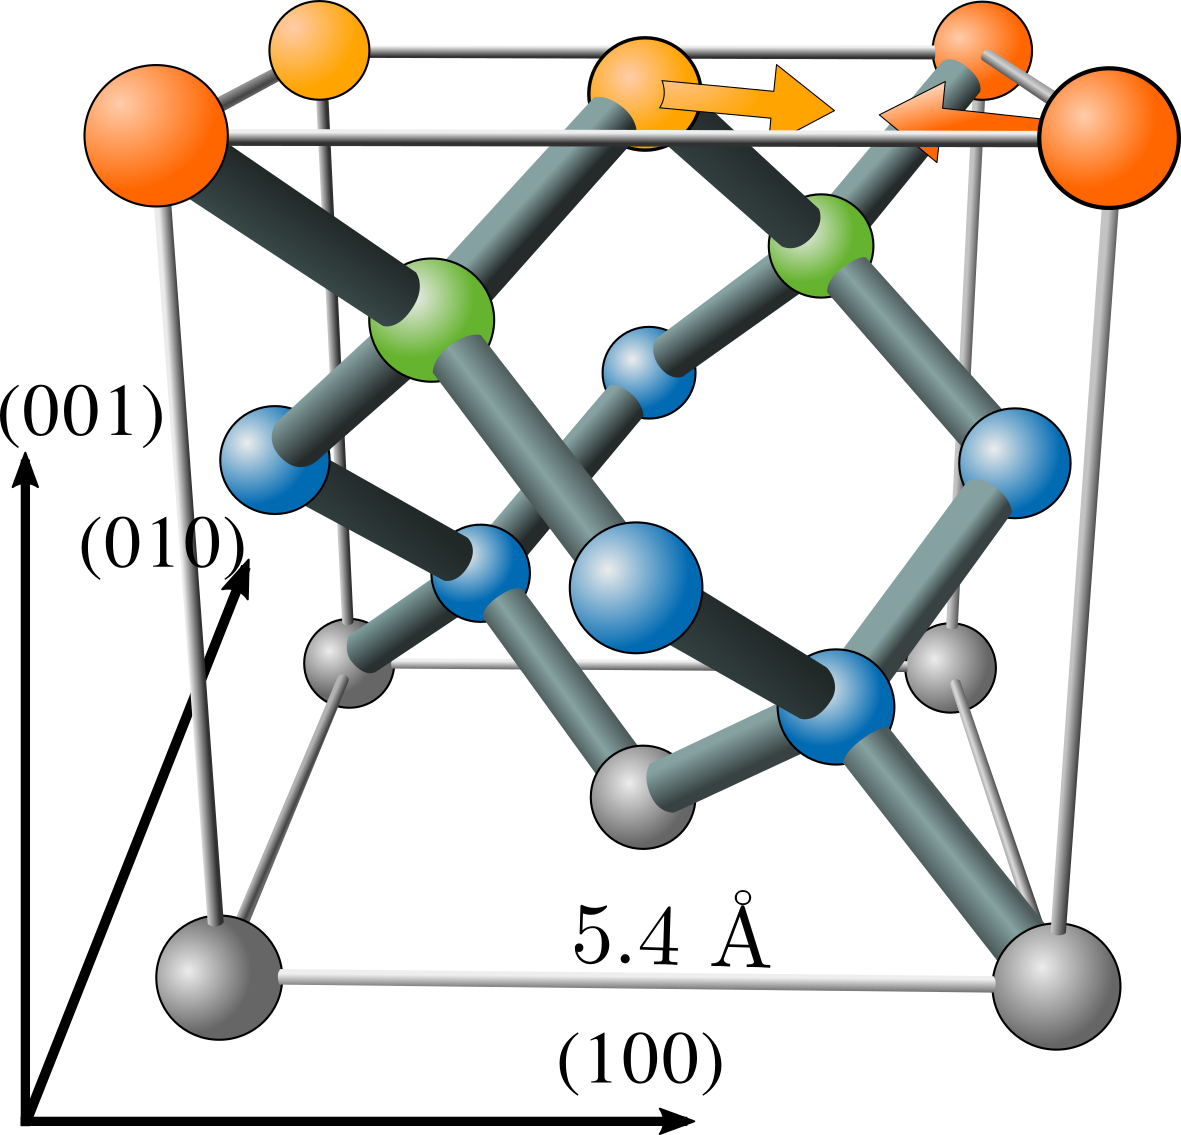
\includegraphics[width=\linewidth]{graphics/Sili-color.png}
		\caption{The crystalline structure of Si in its solid state is shown \cite{sistrucure}.  The orange silicon atoms dimerize during reconstruction of the (001) surface. The coordinate axis are denoted by their Miller indices and normal to their corresponding crystallographic planes. The coloring corresponds with \autoref{Fig::dimer-configs}}
		\label{Fig::SiliconDiamond}
	\end{wrapfigure} \\
	The surface reconstruction with the lowest energy was through theoretical \cite{ramstad1995theoretical, pillay2004revisit, inoue1994order, brand2023critical} and experimental (low energy electron diffraction \cite{matsumoto2003low, kubota1994streak, brand2023critical} and scanning tunnel microscope \cite{wolkow1992direct, tochihara1994low})  methods found to be the $c(4\times 2)$ reconstruction, shown in \autoref{Fig::dimer-configs} (b). It minimizes the interaction energy as well as the surface stress. Si(001) has been mapped onto the exactly solvable two dimensional  Ising model in previous research \cite{brand2023dimer, pillay2004revisit, ihm1983structural, schaller2023sequential, inoue1994order}. In this framework, the dimer interaction is described by an effective coupling $J$ (see \autoref{Section::Ising-Model}). The alternative buckling in both directions suggests an antiferromagnetic interaction along $(110)$, $J_\parallel$, and across $(1\overline{1}0)$, $J_\perp$, the dimer rows, but the interaction across the row is actually ferromagnetic. However, the dimer interactions are strongly anisotropic, with $J_\parallel$ being much larger than $J_\perp$, which causes a guaranteed alternating buckling in $(110)$ direction. The ferromagnetic diagonal interactions $J_\times$ overpower $J_\perp$, so diagonal alignment is preferred, which in turn implies anti-alignment in $(1\overline{1}0)$ direction. It has been suggested that the interaction is of dipole kind \cite{pillay2004revisit}.
	\begin{figure}[htb]
		\begin{subfigure}{0.5\textwidth}
			\centering
			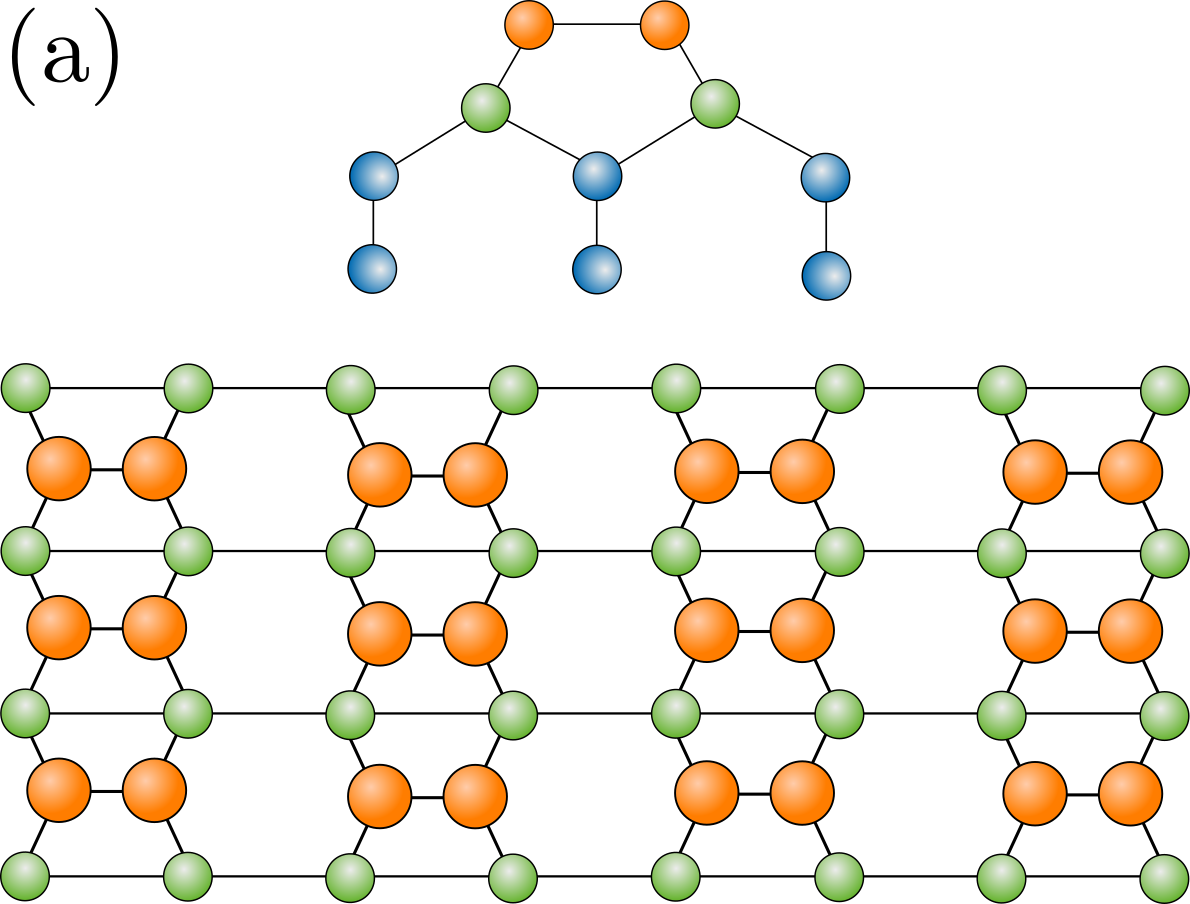
\includegraphics[width=0.8\textwidth]{graphics/p(2x1)-sym-color.png}
			\label{p(2x1)-symmetric}
		\end{subfigure}
		\begin{subfigure}{0.5\textwidth}
			\centering
			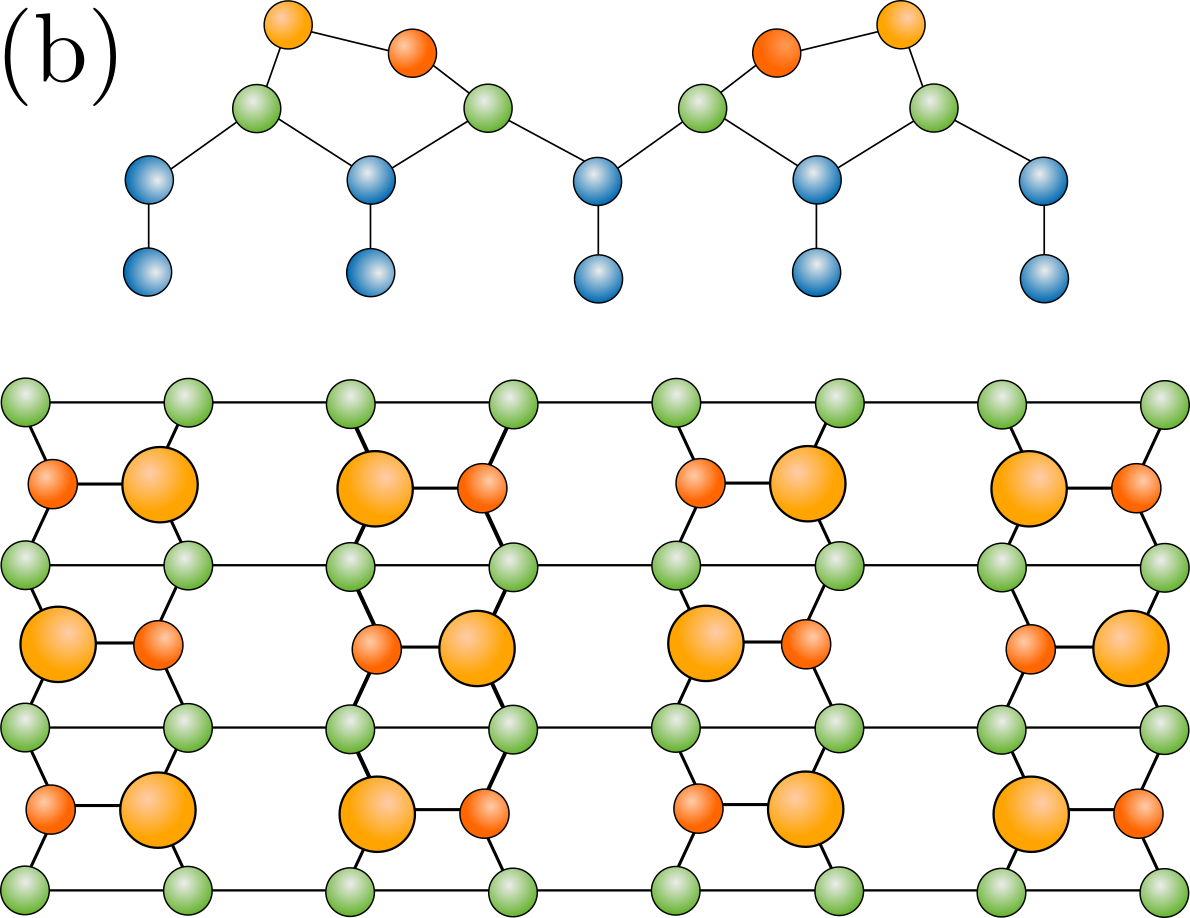
\includegraphics[width=0.8\textwidth]{graphics/c(4x2)-color.png}
			\label{c(4x2)}
		\end{subfigure}
		\caption{ \textbf{(a)}The formation of dimers results in the symmetric $p(2\times1)$ reconstruction and saves a large amount of $1.8~\text{eV}$ per dimer compared to the ideal $p(1\times1)$ structure. \textbf{(b)} The dimers are unstable to vertical buckling. The buckling pattern that was found to have the lowest surface energy is the $c(4\times2)$ reconstruction. The coloring of the silicon atoms corresponds with \autoref{Fig::SiliconDiamond}. Adapted from \cite{brand2023critical}.}
		\label{Fig::dimer-configs}
	\end{figure}
	\section{Phase Transition of the Si(001) Surface}
	Si(001) exhibits an order-disorder phase transition from the disordered $p(2\times1)$ phase shown in \autoref{Fig::dimer-configs} (a) to the ordered $c(4\times2)$ reconstruction at a critical temperature of about $T_c \approx 200~\text{K}$ \cite{tabata1987order, brand2023dimer}. This continuous phase transition will be of central importance in the following discussion. The $p(2\times1)$ structure is short term for the disordered phase since fast flipping of the dimers at a frequency of about $ 10^{11} \text{ Hz}$ \cite{dabrowski1992self} let the system appear to be in the $p(2\times1)$ state at high-temperature measurements. \\
	
	Below $T_c$, the strong anisotropy leads to long streaks of order along the dimer rows and short domains of order across the dimer rows. The parallel dimension of ordered patches is larger than the perpendicular direction by a factor of five \cite{brand2023dimer}. Brand et. al \cite{brand2023critical, brand2023dimer} find good agreement between the experimentally measured static critical properties of the Si(001) phase transition and the Ising universality class. Schaller et. al \cite{schaller2023sequential} employ kinetic Monte Carlo methods to extract a dynamic Kibble-Zurek exponent that matches the expectation for the Ising model. \\% Brand et. al \cite{brand2023dimer} found that the ratio of correlation length amplitudes $\xi^+$ is ${\xi_{\parallel}^+}/{\xi_{\perp}^+} \approx 5.2$. The lattice spacing along the dimer rows is $a_\parallel =	3.84~\text{\AA}$, while it is $a_\perp =	2 a_\parallel =	7.68~\text{\AA}$ across. \\
	
	To understand the transition of the Si(001) surface, some general knowledge of phase transitions will be laid out in the following.
	\chapter{Phase Transitions} \label{Chapter::Phase-Transitions}
	
	The term phase transition describes the process of transition between states of a system by changing an external parameter, like pressure $p$ or temperature $T$. Common types are transitions from an unordered to an ordered state after cooling a system below its critical temperature $T_c$ like the transition from paramagnets to ferromagnets. Intuitively the transitions happen as a result of free energy $F =	U - TS$ minimization. At high temperatures entropy $S$ dominates, leading to unordered states, but at low temperatures the impact of the internal energy $U$ takes over. The minimization of $U$ usually leads to a form of ordering dictated by the microscopic Hamiltonian. \\
	
	%A common type of phase transition is order-disorder transitions when the critical temperature $T_c$ of the system is exceeded, like the transition from ferromagnets to paramagnets. Phenomenologically one could say that the driving force behind the phase transition is the minimization of the free energy $F = U - TS $, with internal energy $U$ and entropy $S$. Below the critical temperature, the internal energy U is minimized leading to a form of ordering dictated by the microscopic Hamiltonian.
	\subsubsection{Mathematical definition}
	Consider a general system in the state $\Omega$ described by the reduced Hamiltonian
	\begin{equation} \label{Eq::General-Hamiltonian}
		\beta H =	\beta \sum_{i}^{d} J_i~ G_i(\Omega) =	\sum_{i}^{d,} K_i ~ G_i(\Omega),
	\end{equation}
	with $\beta =	1 /	k_B T$ being the inverse temperature. The systems energy is characterized by the reduced coupling constants $K_i$ and functionals of the microscopic state $G_i$.
	Let now $N$ denote the number of components, or equivalently the number of lattice sites, and $V$ the volume of the system in question. The \textbf{thermodynamic limit} $N \rightarrow \infty$ and $V \rightarrow \infty$ describes the limit to infinitely large systems while keeping the density $N/V$ constant. For a system dependent on a set of $[K]$, the free energy per site $f$ is defined as
	%In the \textbf{thermodynamic limit} (system volume $V \rightarrow \infty$ or number of sites $N \rightarrow \infty$), we can give a mathematical definition of a phase transition. Consider our system to be dependent on a set of coupling constants $[K]$, which for example can be temperature $T$, pressure $p$ or interaction strength $J$. We define the free energy per site as
	\begin{equation}
		f([K]) =	\lim\limits_{N \rightarrow \infty} \frac{F([K])}{N} ~.
	\end{equation}
	%If the thermodynamic limit exists,
	With $f$ a precise definition of the phase boundary is possible. The $d$ coupling constants $[K]$ span the so called phase space. In this $d$-dimensional phase space, the free energy density $f$ is analytic almost everywhere except from the possibility of non-analyticities at certain points, lines, planes, etc. up to dimensionality $d-1$. The connected areas of analyticity are called \textbf{phases} and non-analyticities with dimension $d-1$ are called \textbf{phase boundaries} or \textbf{critical manifolds}. Since $f$ has to be continuous everywhere, the phase boundaries come in two classes:
	\begin{enumerate}
		\item at least one of the first derivatives $\frac{\partial f}{\partial K_i}$ is discontinuous across the phase transition. This case belongs to the \textbf{first-order phase transition}.
		\item all derivatives $\frac{\partial f}{\partial K_i}$ are continuous. This transition is called the \textbf{continuous phase transition}.
	\end{enumerate}
	The phase transition of the silicon surface belongs to the continuous phase transitions. As the thermodynamic limit is never obtained, descriptions using $f$ are not always reliable. Using the correlation length $\xi$, which simply put describes the spatial extent of fluctuations in the system, a criterion for accurate predictions can be given. If the system size $L$ is much greater than the correlation length $\xi \ll L$ the considered system can be expected to behave according to the ideal behavior described by $f$. \\
	%	The free energy density gives reasonable predictions, when the correlation length $\xi$, which is basically the spatial extent of fluctuations in the system, is much smaller than the system size L, so $\xi \ll L$.
	
	Phase transitions exhibit rich phenomena like the divergence of the correlation length $\xi$ at the critical point. The reason for the universality of this behavior across different systems will be outlined in the next section with the help of renormalization group theory.
	\section{Renormalization Group Considerations} \label{Section::RG}
	The renormalization group (RG) theory is a general framework to study phase transitions and particle physics. It employs scale invariance arguments, meaning the self-similarity characteristics of systems at different length scales, to investigate their properties. It is capable of explaining the origins of singular behavior in phase transitions and universality. These properties are used extensively throughout this research and therefore the fundamentals will be presented briefly.\\
	\begin{figure}[t]
		\centering
		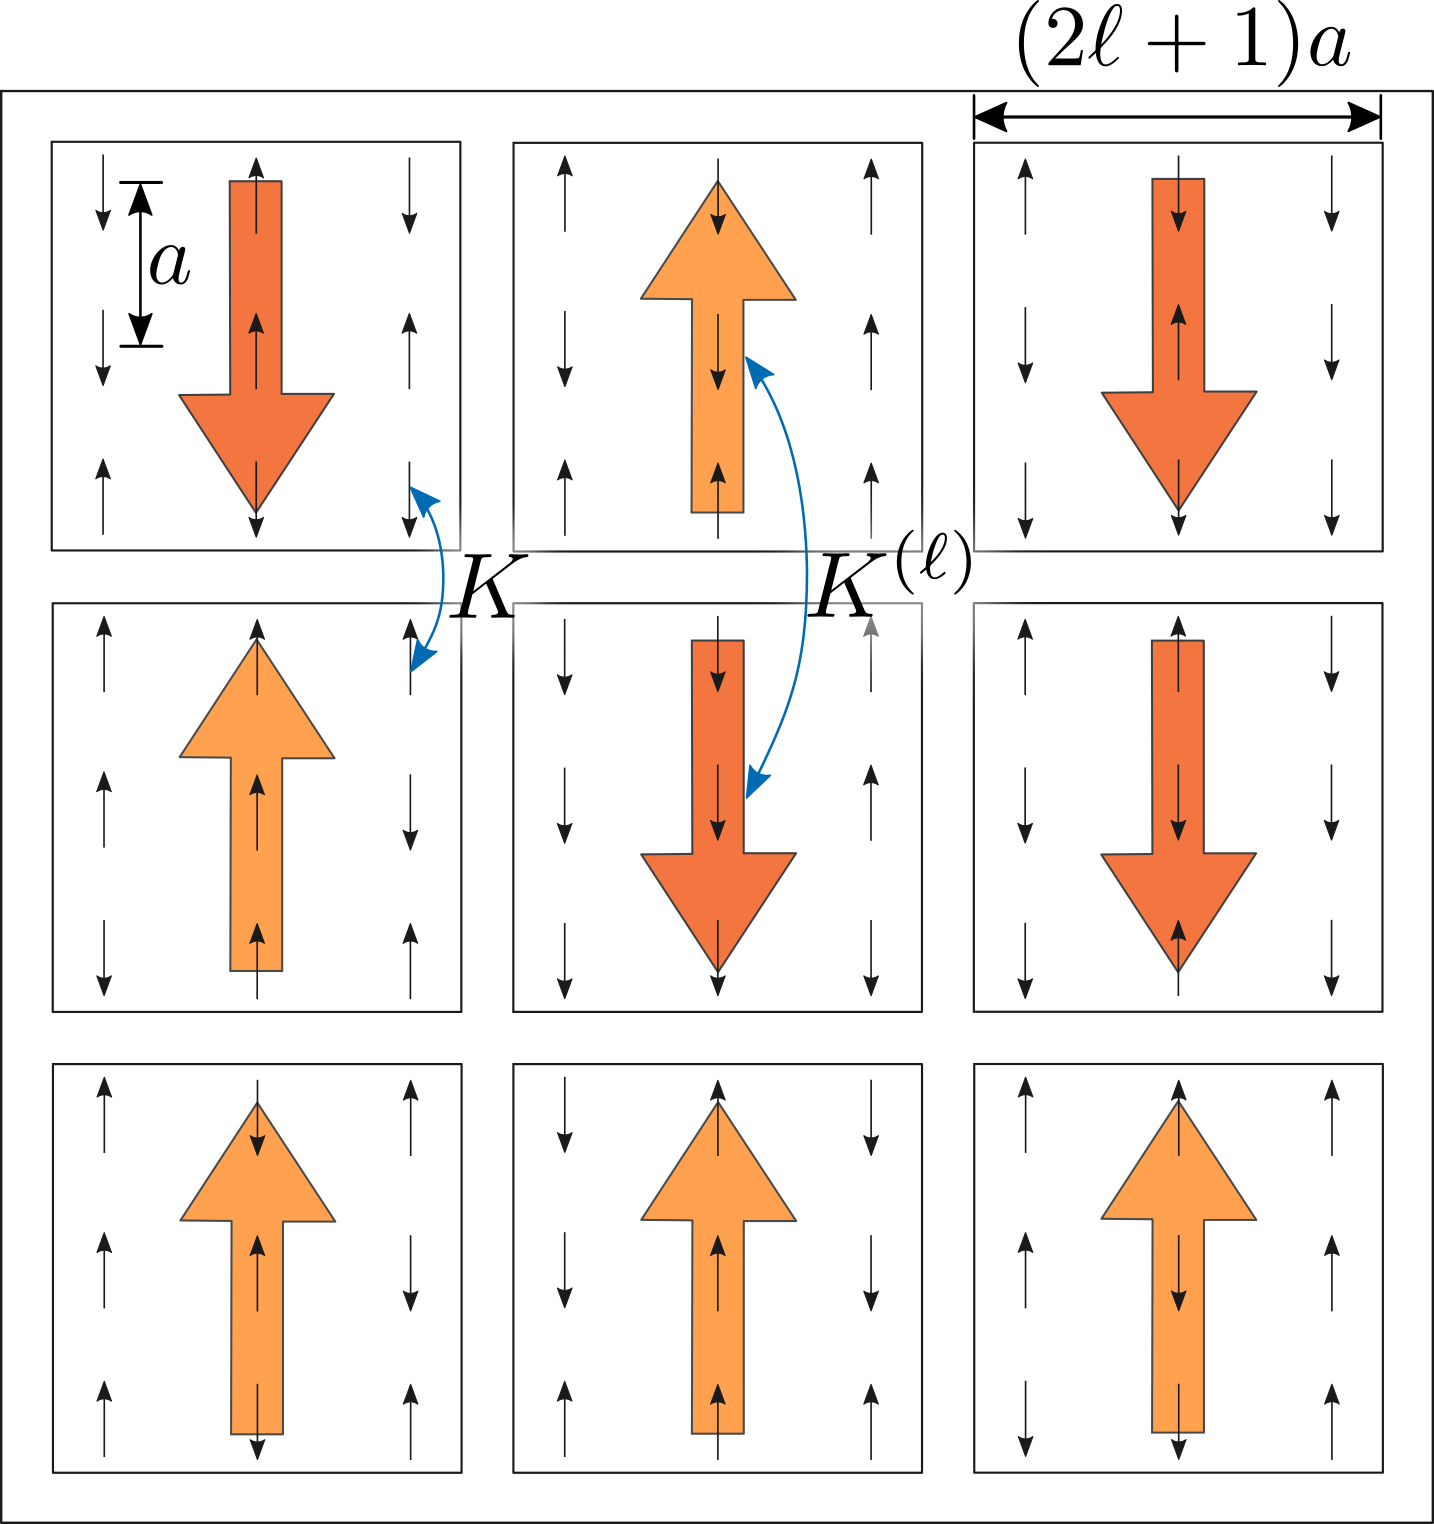
\includegraphics[width=0.7\linewidth]{graphics/RG-Iteration-4.png}
		\caption{In Kadanoff's block spin picture,  blocks $B_{ij}$ of Ising-spins $s_{mn}$ are combined to a composite spin $S^{(\ell)}_{ij}$. One possible RG transformation $R^{(\ell)}$ would be to group $(2\ell + 1)$ spins and map $S^{(\ell)}_{ij} =	\text{sign}\left(\sum_{(m,n) \in B_{ij}} s_{mn} \right)$. The block spin is the standard example for a renormalization group transformation. Under the RG transformation the coupling constants change from $K$ to $K^{(\ell)} =	R^{(\ell)}(K)$.}
		\label{Fig::RG-Iteration}
	\end{figure}
	
	Consider an infinite two dimensional lattice with Ising-like spins $s_{mn}$ on each site, described by a Hamiltonian of form \eqref{Eq::General-Hamiltonian}. The sites are denoted by a tuple of indices $(m,n)$. As an introduction, we follow Kadanoff \cite{kadanoff1966scaling} and divide the system into squares of length $\ell >	1$ in lattice spacing units $a$. The resulting blocks $B_{ij}$ are denoted by a new set of indices $(i,j)$. Their $\ell^2$ spins are mapped onto a single block spin
	\begin{equation}
		S^{(\ell)}_{ij} \propto	\sum_{(m,n) \in  B_{ij}} s_{mn} ~,
	\end{equation}
	The obtained $S_{ij}^{(\ell)}$ define a new Ising system, but on a different length scale with a new lattice spacing $\ell a$ like shown in \autoref{Fig::RG-Iteration}. The proposal is that there exists a set of coupling constants $[K^{(\ell)}]$ so that the total free energy stays the same. In terms of the free energy density we can write
	\begin{equation} \label{free-energy-density}
		f\left([K]\right) =	\ell^{-2} f\left([K^{(\ell)}]\right)~.
	\end{equation}
	The free energy density after the transformation has to increase by a factor $\ell^2$ as it is expressed in an $\ell$-times larger length scale. The same considerations are made for the correlation length, giving
	\begin{equation}
		\xi\left([K]\right) = \ell \xi\left([K^{(\ell)}]\right)~.
	\end{equation}
	In addition to preserving the free energy, an RG transformation has to reflect the symmetries of the system to ensure that the transformed Hamiltonian keeps the original structure. Suppose we know a valid RG transformation $R^{(\ell)}$ so that
	\begin{equation}
		[K^{(\ell)}] =	R^{(\ell)}([K])~.
	\end{equation}
	 (\textcolor{red}{Baustelle})  The starting point is now that, even though each transformation is analytic,
	%the partition function
%	\begin{equation}
%		Z(\{K\})	= \sum_{\{s\}} e^{- \beta H(\{s\}, \{K\})}
%	\end{equation}
%	is a sum of exponentials which are analytic in $[K]$, 
	the singularities of phase transitions can arise after an infinite number of RG iterations. Applying multiple RG transformations traces out a trajectory in coupling constant space $[K^{(\ell_1)}] \rightarrow [K^{(\ell_2)}]  \rightarrow ... \rightarrow [K^{(\ell_n)}]$, called the \textbf{RG flow}. This trajectory is almost always attracted to fixed points. The behavior of a system near a fixed point is the origin of scaling and lets us extract important information, like the shape of the phase diagram.
	
	A fixed point of the RG	map satisfies
	\begin{equation}
		[K^{(*)}] =	R^{(\ell)}\left([K^{(*)}]\right) ~.
	\end{equation}
	At this point the correlation length transforms according to
	\begin{equation}
		\xi\left([K^{(*)}]\right) =	\xi\left([K^{(*)}]\right) / \ell~,
	\end{equation}
	meaning that the correlation length either has to be $0$ or $\infty$. The same is true for the free energy density. In proximity of a fixed point we write the $i$-th coupling constants $K_i$ as
	\begin{equation}
		K_i =	K_i^{(*)} + \delta K_i \qquad \text{and} \qquad K_i^{(\ell)} =	R^{(\ell)}(K_i^{(*)} + \delta K_i) =	K_i^{(*)} + \delta K_i^{(\ell)}~.
	\end{equation}
	The RG Transformation of $K_i$ is in general dependent on all $K$ so that
	\begin{equation}
		K^{(\ell)}_i =	K^{(\ell)}_i([K]) =	K^{(\ell)}_i(K_1^{(*)} + \delta K_1, K_2^{(*)} + \delta K_2, ...).
	\end{equation}
	The Taylor expansion of $K_i^{(\ell)}$ around the fixed point $[K^{(*)}]$ yields the linearized RG Transformation
	\begin{equation} \label{Eq::linearized-RG}
		K_i^{(\ell)} =	K_i^{(*)} + \sum_j \frac{\partial K_i^{(\ell)}}{\partial K_j} \bigg |_{K_j = K_j^{(*)}} \delta K_j + O((\delta K_j)^2) = K_i^{(*)} + \delta K_i^{(\ell)} + O((\delta K_j)^2) ~.
	\end{equation}
	Omitting terms quadratic or higher in $\delta K_j$ identifies
	\begin{equation}
		\delta K_i^{(\ell)} =	\sum_j \frac{\partial K_i^{(\ell)}}{\partial K_j} \bigg |_{K_j = K_j^{(*)}} \delta K_j~.
	\end{equation}
	We write down the partial derivatives as a matrix
	\begin{equation}
		M^{(\ell)}_{ij} =	\frac{\partial K_i^{(\ell)}}{\partial K_j} \bigg |_{K_j = K_j^{(*)}}~,
	\end{equation}
	and construct an eigenvalue problem
	\begin{equation} \label{ev-problem}
		M^{(\ell)} \boldsymbol{k}_{\sigma} =	\lambda_{\sigma}^{(\ell)} \boldsymbol{k}_{\sigma}~,
	\end{equation}
	where $\sigma$ labels the eigenvalues. The eigenvectors $\boldsymbol{k}_\sigma$ are printed bold.  Because two consecutive RG Transformations by $l_1$ and $l_2$ have to yield the same result as one  by $l_1l_2$, we know that
	\begin{equation}
		M^{(\ell_1)}M^{(\ell_2)} = M^{(\ell_2)}M^{(\ell_1)} =		M^{(\ell_1\ell_2)}~.
	\end{equation}
	Because the matrices commute the eigenvalues satisfy \textcolor{red}{(?)}
	\begin{equation}
		\lambda^{(\ell_1)}_{\sigma} \lambda^{(\ell_2)}_{\sigma} =	\lambda^{(\ell_1\ell_2)}_{\sigma} ~.
		\label{ev-equation}
	\end{equation}
	Setting $l_2 = 1$ gives $\lambda^{(\ell_1)}_{\sigma} \lambda^{(1)}_{\sigma} =	\lambda^{(\ell_1)}_{\sigma}$, which lets conclude that $\lambda^{(1)}_{\sigma} =	1$. Differentiating \autoref{ev-equation} with respect to $l_2$ yields
	%	\begin{equation}
		%		\begin{split}
			%			\frac{\text{d}}{\text{d}l_2} \left(\lambda_{l_1}^{(\sigma)} \lambda^{(\ell_2)}^{(\sigma)}\right) &= 	\frac{\text{d}}{\text{d}l_2} \lambda_{l_1l_2}^{(\sigma)} \\
			%			\lambda_{l_1}^{(\sigma)}  \left(\frac{\text{d}}{\text{d}l_2} \lambda^{(\ell_2)}^{(\sigma)}\right) +  			  \left( \frac{\text{d}}{\text{d}l_2} \lambda_{l_1}^{(\sigma)}\right) \lambda^{(\ell_2)}^{(\sigma)} &= l_1 \frac{\text{d}}{\text{d}(l_1l_2)} \lambda_{l_1l_2}^{(\sigma)} \\
			%			\left(\frac{\text{d}}{\text{d}l_2} \lambda^{(\ell_2)}^{(\sigma)}\right) \lambda^{(\ell_1)}^{(\sigma)}   &= l_1 \frac{\text{d}}{\text{d}(l_1l_2)} \lambda_{l_1l_2}^{(\sigma)}	~.
			%		\end{split}
		%	\end{equation}
	\begin{equation}
		\frac{\text{d}}{\text{d}l_2} \left(\lambda^{(\ell_1)}_{\sigma} \lambda^{(\ell_2)}_{\sigma}\right) = \lambda^{(\ell_1)}_{\sigma}  \left(\frac{\text{d}}{\text{d}l_2} \lambda^{(\ell_2)}_{\sigma}\right) +  			  \left( \frac{\text{d}}{\text{d}l_2} \lambda^{(\ell_1)}_{\sigma}\right) \lambda^{(\ell_2)}_{\sigma} 	= \left(\frac{\text{d}}{\text{d}l_2} \lambda^{(\ell_2)}_{\sigma}\right) \lambda^{(\ell_1)}_{\sigma}
	\end{equation}
	for the left hand side and
	\begin{equation}
		\frac{\text{d}}{\text{d}l_2} \lambda^{(\ell_1 \ell_2)}_{\sigma} =	\frac{\text{d}}{\text{d}(l_2 l_1)} \lambda^{(\ell_1 \ell_2)}_{\sigma} \frac{\partial}{\partial l_2} (l_1 l_2) =	l_1 \frac{\text{d}}{\text{d}(l_1l_2)} \lambda^{(\ell_1 \ell_2)}_{\sigma}
	\end{equation}
	for the right hand side. By setting $l_2 =	1$ the differential equation
	\begin{equation}\label{RG-diff}
		\frac{\text{d}}{\text{d}l_2} \lambda^{(\ell_2)}_{\sigma} \bigg |_{l_2 =	1} \lambda^{(\ell_1)}_{\sigma}  = y_\sigma \lambda^{(\ell_1)}_{\sigma} = l_1 \frac{\text{d}}{\text{d}l_1} \lambda^{(\ell_1)}_{\sigma}
		%\quad \Rightarrow \quad \frac{\text{d}}{\text{d}l_1} \lambda^{(\ell_1)}_{\sigma} =	\frac{y_\sigma}{l_1} \lambda^{(\ell_1)}_{\sigma} ~.
	\end{equation}
	with
	\begin{equation}
		y_\sigma = \frac{\text{d}}{\text{d}l_2} \lambda^{(\ell_2)}_{\sigma} \bigg |_{l_2 =	1}
	\end{equation}
	is obtained.
	A solution to Eq.~{\eqref{RG-diff}} is
	\begin{equation} \label{ev-form}
		\lambda^{(\ell)}_{\sigma} = \ell^{y_\sigma}~,
	\end{equation}
	with $y_\sigma$ being independent of $\ell$. This is an important result on the way to show the origin of scaling. The $\boldsymbol{k}_{\sigma}$ are vectors in the coupling constant space, so \autoref{ev-problem} indicates that some $\delta K_i$ grow and some shrink when applying RG transformations, depending on the eigenvalue $\lambda^{(ell)}l_{\sigma}$. Three cases are distinguished:
	\begin{enumerate}
		\item \textbf{Relevant} directions and eigenvalues:	$|\lambda^{(\ell)}_{\sigma}| > 1$, meaning that $y_\sigma > 0$ and $\delta K$ in direction of $\boldsymbol{k}_{\sigma}$ grow.
		\item \textbf{Irrelevant} directions and eigenvalues:	$|\lambda^{(\ell)}_{\sigma}| < 1$, meaning that $y_\sigma < 0$ and $\delta K$ in direction of $\boldsymbol{k}_{\sigma}$ shrink.
		\item \textbf{Marginal} directions and eigenvalues:	$|\lambda^{(\ell)}_{\sigma}| = 1$, meaning that $y_\sigma = 0$ and $\delta K$ in direction of $\boldsymbol{k}_{\sigma}$ do not change.
	\end{enumerate}
	After many iterations, only the relevant eigenvalues will be important, as shrinking $\delta K_i$ won't impact the RG flow significantly. If we differ from the fixed point in a relevant direction, the differences to the fixed point will become larger and the RG transformation flow will move away from the fixed point. Deviations in irrelevant direction will flow into the fixed point. \\
	
	A simplified understanding can be achieved for a system satisfying
	\begin{equation}
		\frac{\partial K_i^{(\ell)}}{\partial K_j} \bigg |_{K_j = K_j^{(*)}} = \delta_{ij} \frac{\partial K_j^{(\ell)}}{\partial K_j} \bigg |_{K_j = K_j^{(*)}}~,
	\end{equation}
	so that $M^{(\ell)}$ becomes diagonal and the eigendirections $\boldsymbol{k}_{\sigma}$ point along the axes of the phase space defined by $[K]$. If the eigenvalue $\lambda^{(\ell)}_{\sigma}$ to $\boldsymbol{k}_{\sigma}$ is larger than one, the coupling $K_\sigma$ will grow. In this case $K_\sigma$ would be a relevant coupling constant. \\
	
	Consider a system with only one coupling constant $K = J /	k_B T$, or equivalently just the temperature $T$, and choose $T$ in the vicinity of a fixed point $T^{(*)}$. Apply a RG transformation to $T$ and consider the difference
	\begin{equation} \label{temp-difference}
		T^{(\ell)} - T^{(*)} =	R^{(\ell)}(T) - T^{(*)}~.
	\end{equation}
	Using Eq.~\eqref{Eq::linearized-RG} we can rewrite
	\begin{equation}
		R^{(\ell)}(T) =	T^{(*)} + \delta T^{(\ell)} =	T^{(*)} + \frac{\partial T^{(\ell)}}{\partial T} \bigg |_{T =	T^{(*)}} \delta T =	T^{(*)} + \lambda^{(\ell)} \delta T~,
	\end{equation}
	since $M^{(\ell)}$ has only one component and $\delta T$ is therefore automatically in eigenvector direction with eigenvalue
	\begin{equation} \label{Eq::Eigenvalue-from-RG}
		\lambda^{(\ell)} =	\frac{\partial R^{(\ell)} (T)}{\partial T} \bigg|_{T =	T^{(*)}}~.
	\end{equation}
	Eq.~\eqref{temp-difference} then becomes
	\def\equationautorefname{Eq.}
	\begin{equation} \label{Eq::epsilon-RG-scaling}
		\varepsilon^{(l)} =	\lambda^{(\ell)} \varepsilon \overset{\text{\autoref{ev-form}}}{=} \varepsilon l^{y_\varepsilon}~,
	\end{equation}\def\equationautorefname{Equation}
	in terms of the \textbf{reduced temperature} $ \varepsilon =	\frac{T - T^{(*)}}{T^{(*)}}$. After $n$ RG iterations this gives
	\begin{equation}
		\varepsilon^{(nl)} = \left( l^{y_\varepsilon}	\right)^n \varepsilon~.
	\end{equation}
	Now consider again how the correlation length transforms after $n$ RG transformations
	\begin{equation} \label{xi-behavior}
		\xi(\varepsilon) =	l^n \xi(\varepsilon^{nl}) =	l^n \xi( l^{ny_\varepsilon} \varepsilon)~.
	\end{equation}
	Substituting $\tau =	l^{ny_\varepsilon} \varepsilon$ into Eq.~\eqref{xi-behavior} yields
	\begin{equation} \label{Eq::RG-xi-scaling}
		\xi(\varepsilon) =	\tau^{1 / y_\varepsilon} \varepsilon^{-1/ y_\varepsilon} \xi(\tau) =:	\varepsilon^{-{1}/{y_\varepsilon}} F_\xi (\tau^{1 /	y_\varepsilon})~,
	\end{equation}
	showing that the correlation length diverges at the critical point $\varepsilon \rightarrow 0$. This is the origin of the singular behavior of phase transitions! Using Eq. \eqref{Eq::epsilon-RG-scaling} and \eqref{Eq::Eigenvalue-from-RG}, a valid RG transformation $R^{(\ell)}$ directly provides the exponent $y_\varepsilon$ via
	\begin{equation}
		y_\varepsilon =	\frac{1}{l} \ln \left(\frac{\partial R^{(\ell)} (T)}{\partial T} \bigg|_{T	=	T^{(*)}}\right)~.
	\end{equation}
	The only restrictions that were imposed on $R^{(\ell)}$ were that it keeps the total free energy invariant, and that it reflects the symmetries of the system. These properties do not depend on the microscopic details of the considered system and that is the reason for universality.
	\section{Universality and Static Scaling} \label{Section::Universality}
	The last section traced the origin of universality and scaling in phase transitions. This section will deal with the term universality and its implications in more detail. \\
	
	Scaling laws like Eq.~\eqref{Eq::RG-xi-scaling} can be derived for different system quantities. In the context of phase transitions, \textbf{static scaling} means the power law dependence of a system quantity \textbf{in equilibrium}, like the correlation length $\xi$, on a coupling parameter, like the temperature $T$. The exponent of this power law is called the \textbf{critical exponent}. Some important scaling relations are shown in \autoref{Table::Scaling-Laws}. Comparing the scaling law of $\xi$ with Eq.~\eqref{Eq::RG-xi-scaling} identifies
	\begin{equation}
		\frac{1}{y_\varepsilon} = \nu ~.
	\end{equation}
	%	\begin{itemize}
		%		\item the specific heat $\boldsymbol{C_H}$: $T_c C_H \approx A^{\pm} |\varepsilon|^{-\alpha}$,
		%		\item the order parameter $\boldsymbol{\Psi}$ or $\boldsymbol{M}$: $|M| \approx B |\varepsilon|^{-\beta}$,
		%		\item the susceptibility $\boldsymbol{\chi}$: $\chi \approx C^{\pm} |\varepsilon|^{-\gamma}$,
		%		\item and the correlation length $\boldsymbol{\xi}$ : $\xi \approx f^{\pm} |\varepsilon|^{-\nu}$.
		%	\end{itemize}
	\begin{table}[h]
		\centering
		\caption{Some important scaling laws are summarized in the notation of \cite{pelissetto2002critical}, except for $\xi$. The universal critical exponents $\alpha, \beta,$ etc. are the same above and below the phase transition. In contrary, the nonuniversal critical amplitudes may differ at different sides of the critical point. Hence, they are labeled with a superscript $\pm$. The dimensionality is denoted by $d$.}
		\begin{tabular}{l c l}
			\toprule
			Name  & $\quad$ Symbol $\quad$ & Scaling \\
			\midrule
			specific heat & $C_H$ & $T_c C_H \approx A^{\pm} |\varepsilon|^{-\alpha}$ \\
			order parameter & $\Psi, M$ & $|M| \approx B |\varepsilon|^{-\beta}$ \\
			susceptibility & $\chi$ & $\chi \approx C^{\pm} |\varepsilon|^{-\gamma}$ \\
			correlation length & $\xi$ & $\xi \approx \xi^{\pm} |\varepsilon|^{-\nu}$ \\
			two-point correlation function & $C(\vec{r})$& $C(\vec{r}) \propto |\vec{r}|^{- d + 2 - \eta}$ \\
			\bottomrule
		\end{tabular}
		\label{Table::Scaling-Laws}
	\end{table}
	The prefactors of the power laws are called the \textbf{critical amplitudes} and $\nu, \alpha, $ etc. are the mentioned critical exponents. The superscript $\pm$ denotes whether the phase transition is approached from below $(-)$ or above $(+)$ the critical temperature $T_c$. The critical exponents are the same on both sides of the transition, but the amplitudes vary. \\
	
	These scaling laws are only valid in the thermodynamic limit for $\varepsilon \rightarrow 0$ as the derivation in \autoref{Section::RG} assumed that the system is in the vicinity of a critical point. Otherwise they exhibit \textbf{corrections to scaling} \cite{wegner1972corrections, pelissetto2002critical} that result out of irrelevant and marginal eigenvalues of the RG transformations as well as \textbf{finite-size} corrections \cite{domb1983vol8, goldenfeld2018lectures}. \\
	
	Systems that share the same set of critical exponents belong to the same \textbf{universality class}. \autoref{Section::RG} showed that the exponents can be calculated solely from the RG transformation which suggests that systems with similar transformations exhibit similar critical behavior. Indeed it is found that the universality class of a system only depends on
	\begin{itemize}
		\item the \textbf{symmetry group} of the system Hamiltonian,
		\item the \textbf{dimensionality} of the problem,
		\item and whether the \textbf{interaction} between the components is \textbf{short-ranged}, usually meaning that the interaction at distance $r$ decays faster than $r^{-2}$.
	\end{itemize}
	In contrast to the critical exponents, the critical amplitudes are not universal, but their ratios, for example $\xi^+/\xi^-$, are.\\
	
	The concept of universality is very useful to investigate real systems at the critical point. As a result of scale invariance and self similarity, the microscopic dynamics of a system become irrelevant at $\varepsilon =	0$. Its behavior can then be approximated by a simplified, in the best case exactly solvable, model. \\
	
	The extraction of critical exponents is notoriously difficult for various reasons, one being the inaccessibility of the thermodynamic limit, another \textbf{critical slowing down} (see \autoref{Section::Dynamic-Scaling}). The following section will explain the mentioned finite size corrections to static scaling and illustrate how they can be used to analyze critical exponents.
	\section{Finite-size Scaling and Critical Exponent Extraction} \label{Section::FSS}
	The upcoming numerical implementation is limited in system size and computation time. The topic of \textbf{finite-size scaling }(FSS) analyzes the deviations from finite systems from the ideal behavior. It can be used to determine critical properties and will be useful when evaluating the simulation. \\
	
	The system size $L$ transforms after RG transformation according to
	\begin{equation}
		R^{(\ell)}(L) =	L^{(l)} =	L /	l ~,
	\end{equation}
	analogous to the correlation length. Extending the transformation of the free energy density of Eq.~\eqref{free-energy-density} by a dependence on the system size yields
	%	Recall how the free energy density \autoref{free-energy-density} transforms and that it depends on the system size $L = l L^{(l)}$:
	\begin{equation}\label{Eq::FSS-free-energy-scaling}
		f\left([K], L^{-1}\right) =	l^{-2} f\left([K^{(l)}], {L^{(l)}}^{-1}\right) = l^{-2} f\left([K^{(l)}], l{L}^{-1}\right)	 ~,
	\end{equation}
	the finite-size scaling of $f$.
	Let $K_1 =	\varepsilon$ be the reduced temperature. Close to the critical point Eq. \eqref{Eq::epsilon-RG-scaling} can be used to write \eqref{Eq::FSS-free-energy-scaling} in terms of eigenvalues
	\begin{equation}
		f\left(\varepsilon, K_2, ..., L^{-1}\right) = l^{-2} f\left(\varepsilon l^{y_\varepsilon}, K_2 l^{y_2}, ..., l{L}^{-1}\right)	 ~.
	\end{equation}
	The system size behaves like a relevant coupling constant with an eigenvalue of
	\begin{equation}
		\lambda_L =	1~, \qquad \text{implying that} \qquad y_L =	1 ~.
	\end{equation}
	This means that the system size has to be tuned to criticality for the phase transition to occur. Like $\varepsilon$, the inverse system size has to be set zero $L^{-1} =	0$ which is equivalent to taking the thermodynamic limit. As a result, real, finite systems deviate from the behavior that scaling laws dictate. The actual correlation length cannot outgrow the system size $\xi_L \leq L$ and so the divergence of $\xi$ is rounded at the phase transition. Additionally,  the peak of $\xi_L(T)$ is shifted \cite{domb1983vol8}. The ideal behavior of $\xi$ is sketched versus the behavior of a finite system in  \autoref{xi-divergence-FS}. \\
	
	\begin{figure}[htp]
		\centering
		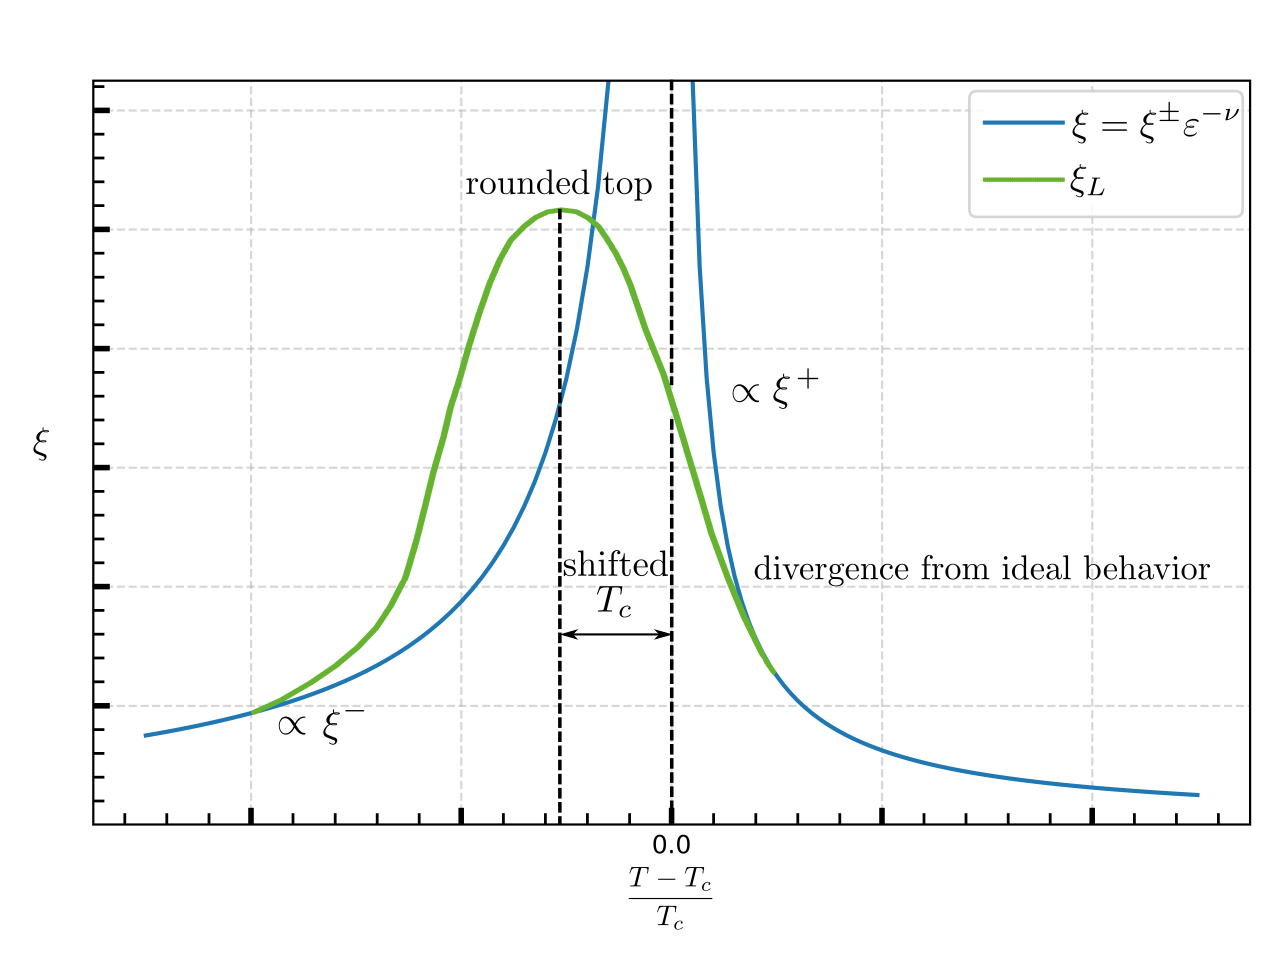
\includegraphics[width=0.7\linewidth]{graphics/xi-divergence5.png}
		\caption{The equilibrium correlation length $\xi$ is shown versus the reduced critical temperature. In the thermodynamic limit, $\xi$ diverges at the critical point according to a power law, as depicted by the blue line. For finite systems, the singularity of $\xi$ appears rounded as shown by the green curve. The peak position is shifted to an effective critical temperature.}
		\label{xi-divergence-FS}
	\end{figure}
	Now consider Eq.~\eqref{xi-behavior} extended by $L$-dependence reading
	\begin{equation}
		\xi(\varepsilon, L^{-1}) =	l \xi (\varepsilon l^{y_\varepsilon}, l L^{-1}) = \varepsilon^{-\nu} F_\xi (L^{-1} \varepsilon^{-\nu})~,
	\end{equation}
	with $F_\xi$ as in Eq.~\eqref{Eq::RG-xi-scaling}. Introducing a new scaling function $F' =	(L \varepsilon^\nu)^{-1} F_\xi$ yields
	\begin{equation}
		\xi(\varepsilon, L^{-1}) = \varepsilon^{-\nu} (L\varepsilon^\nu) F' (L \varepsilon^{\nu}) =	L	F'(L \varepsilon^\nu)~.
	\end{equation}
	In the limit $L \rightarrow \infty$ and close to $\varepsilon =	0$, $\xi$ has to scale like $\xi(\varepsilon, 0) \propto \varepsilon^{-\nu}$ implying that
	\begin{equation}
		\lim_{L \rightarrow \infty} \lim_{\varepsilon \rightarrow 0} F'(L \varepsilon^\nu) \propto (L \varepsilon^\nu)^{-1}~.
	\end{equation}
	The correlation length is capped for finite $L$ so that at the critical point $\xi(0, L^{-1}) \propto L$. For $F'$ this means
	\begin{equation}
		\lim_{\varepsilon \rightarrow 0} F'(L\varepsilon^\nu) \propto \text{const.}~,
	\end{equation}
	showing that the scaling function does not diverge. Therefore, a Taylor expansion around $\varepsilon =	0$ is reasonable and gives
	\begin{equation} \label{Equation::FSS-Scaling-L/xi}
		\frac{L}{\xi(\varepsilon, L^{-1})} =	A + B \varepsilon L^{1/\nu} + O(\varepsilon^2)~. 
	\end{equation}
	This equation is an important result since it can be used to calculate two central quantities. Firstly, curves of $L/\xi(\varepsilon, L^{-1})$ for different $L$ intersect at the critical point $\varepsilon = 0$. Hence, by determining this intersection one can extract the critical temperature $T_c$, which is usually not known a priori. Secondly, by computing the gradient
	\begin{equation}
		\frac{\partial}{\partial \varepsilon} \left(\frac{L}{\xi(\varepsilon, L^{-1})}\right) =	B L^{1/\nu}
	\end{equation}
	for various $L$, one can determine the critical exponent $\nu$. This method is easier than, for example, trying to fit to the original scaling law Eq.~\eqref{Eq::RG-xi-scaling} because of the reasons mentioned at the end of \autoref{Section::Universality}.
	\subsection{Binder Cumulant} \label{Sec::Binder-Cumulant}
	FSS scaling laws like Eq.~\eqref{Equation::FSS-Scaling-L/xi} can be derived for any thermodynamic quantity \cite{pelissetto2002critical, blote1995ising}. The Binder cumulant $U_L$, introduced by K. Binder in \cite{binder1981finite}, is frequently used to investigate simulations. It is defined as
	\begin{equation} \label{Eq::Def-Binder-Cum}
		U_L =	\frac{\langle M_L^4 \rangle}{\langle M_L^2 \rangle^2}~,
	\end{equation}
	with $M_L$ being the lattice average 
	\begin{equation} \label{Eq::lattice-average}
		M_L	=	L^{-2} \sum_i s_i
	\end{equation}
	of a system of size $L$. The lattice sites are again characterized by $s_i$. The ensemble average $\left\langle~\cdot~\right \rangle$ denotes the mean of infinitely many system realizations. Its finite size scaling is analogous to Eq.~\eqref{Equation::FSS-Scaling-L/xi} given by
	\begin{equation}
		U_L =	U^* + U \varepsilon L^{1/\nu} \left(1 + W L^{-\omega} + ...\right)~,
	\end{equation}
	including corrections resulting out of the largest irrelevant eigenvalue $1/|y_1| =	\omega $.
	To extract the critical exponent $\nu$ a linear fit to
	\begin{equation} \label{Eq::FSS-dU_dT}
		\ln \left(\frac{\partial U_L}{\partial \varepsilon}\right) \approx	\ln \left(U L^{1/\nu} \right) =	\ln (U) + \frac{1}{\nu} \ln (L) ~.
	\end{equation}
	is performed. For Ising lattices, it can be shown \cite{binder1981finite} that the cumulant has a value of $U_L=1$ far below the critical temperature and approaches $U_L =	3$ for high temperatures. In between, it exhibits an intersection at $U_L =	U^*$. These implications can be generalized to spin dimensionalities larger than one \cite{binder1981critical} and have been shown to be consistent with the XY model \cite{landau1983non, bernreuther1988investigation}. The Binder cumulant is generally easy to compute and extract.
	\section{Dynamic Scaling and the Kibble-Zurek Mechanism} \label{Section::Dynamic-Scaling}
	\subsection{The Relaxation Time $\tau$ and the Critical Exponent $z$}
	With the Binder cumulant we acquired a way to extract the static scaling exponent $\nu$. Aside static scaling, \textbf{dynamic critical phenomena} are of central importance to describe phase transitions. Dynamic scaling describes how much time fluctuations in systems take to equilibrate. This time is called the  \textbf{relaxation time} $\tau_k$ and it is usually specified for different length scales with the wavenumber $k$. The zero wavenumber relaxation time $\tau_0 =	\tau$ quantifies relaxation on the largest length scales. Its scaling \cite{hohenberg1977theory}
	\begin{equation}
		\tau =	\tau_\xi \xi(\varepsilon)^z
	\end{equation}
	defines a new \textbf{dynamic critical exponent} z, as well as a proportionality constant $\tau_\xi$. \\
	
	Plugging in the known scaling of $\xi(\varepsilon)$ from \autoref{Section::Universality} yields
	\begin{equation}
		\tau = \tau_\xi \xi(\varepsilon)^z =\tau_\xi	\left(\xi^{\pm} |\varepsilon|^{-\nu}\right)^z :=	\tau_\varepsilon |\varepsilon|^{-\nu z} ~.
	\end{equation}
	As the correlation length diverges, so does the relaxation time. Interpreting $\xi$ as a characteristic length at which system components are still influenced by each other gives an intuitive explanation for this divergence. The maximum speed for the propagation of interactions in the system is the respective speed of sound. Even the speed of sound would need an infinite amount of time to cover the diverging correlation distance. In practice the propagation will take much more time. This is the in \autoref{Section::Universality} mentioned phenomenon of critical slowing down. As a system approaches $\varepsilon \rightarrow 0$, it takes longer and longer to equilibrate. It then becomes a computational challenge to relax large systems. But since static scaling laws describe quantities in equilibrium and are only valid in the thermodynamic limit for $\varepsilon \rightarrow 0$, large, critical systems have to be considered.  This dilemma is partially solved by the finite size techniques of \autoref{Section::FSS}. \\
	
	Analogous to the static phenomena, the dynamic scaling is also universal. The static and dynamic universality classes are not independent, but the dynamic ones form subgroups of the static universality classes. Besides the usual indicators described in \autoref{Section::Universality}, the conservation laws that are fulfilled by the system, as well as Poisson-bracket relations between the order parameter and the conserved densities are decisive for the respective universality class. The important anisotropic Ising model is part of Model A as specified by Hohenberg and Halperin \cite{hohenberg1977theory}. Its dynamic critical exponent can be expressed in terms of
	\begin{equation} \label{Eq::Model-A-z}
		z =	2 + c \eta ~,
	\end{equation}
	with $\eta$ as in \autoref{Table::Scaling-Laws} and $c$ a constant to be determined.
	\subsection{Quenches and the Freeze-out of Domains} \label{Section::Quenches}
	Systems like the Si(001) surface that exhibit order-disorder phase transitions usually have multiple possible orderings in the low temperature state. Boundaries between domains of different order, also called domain walls, are stable topological defects. The \textbf{Kibble-Zurek mechanism} (KZM) \cite{kibble1976topology, zurek1985cosmological, zurek1996cosmological} describes the behavior of $\xi$ after driving a system through its phase transition. It directly relates the correlation length to the static and dynamic critical exponents $\nu$ and $z$ through a scaling law that has been verified in numerous experiments \cite{ruutu1996vortex, ulm2013observation, pyka2013topological}. Therefore, it can be used to describe the final density of topological defects. The KZM shall be a central point of the upcoming investigations and will be explained in the following. \\
	
	We will solely consider linear quenches, concretely the cool down of a system linear in time $t$. The speed of cooling is characterized by the \textbf{quench timescale} $\tau_Q$ defined by
	\begin{equation} \label{Eq::Linear-Quench}
		\varepsilon(t) =	\frac{t}{\tau_Q}~.
	\end{equation}
	For slow quenches sufficiently far away from the critical point, the system will evolve adiabatically, meaning that thermodynamic quantities like $\xi$ assume their equilibrium values. As the system approaches the phase transition at $t=0$, the derivative
	\begin{equation}
		\frac{\partial}{\partial t} \xi(\varepsilon(t)) =	- \nu f^{\pm} \frac{(\tau_Q)^\nu}{t^{-(\nu + 1)}}
	\end{equation}
	diverges and at some point will eventually outgrow the reaction capability of the system. The actual correlation length will diverge from its equilibrium behavior like shown in \autoref{Fig::Freeze-out}. The timepoint $\hat{t}$ of divergence from the equilibrium behavior is called the \textbf{freeze-out} since the current state of the system effectively becomes frozen in comparison with the equilibrium values. The KZM states that the freeze-out roughly happens at
	% when the current relaxation time $\tau$ equals the time until the crossing of the critical point $\hat{t}$, defining
	\begin{equation}
		\tau(\hat{t}) = \hat{t}~.
	\end{equation}
	At this point, the system won't have time to equilibrate until the critical point is passed.
	\begin{figure}[t!]
		\centering
		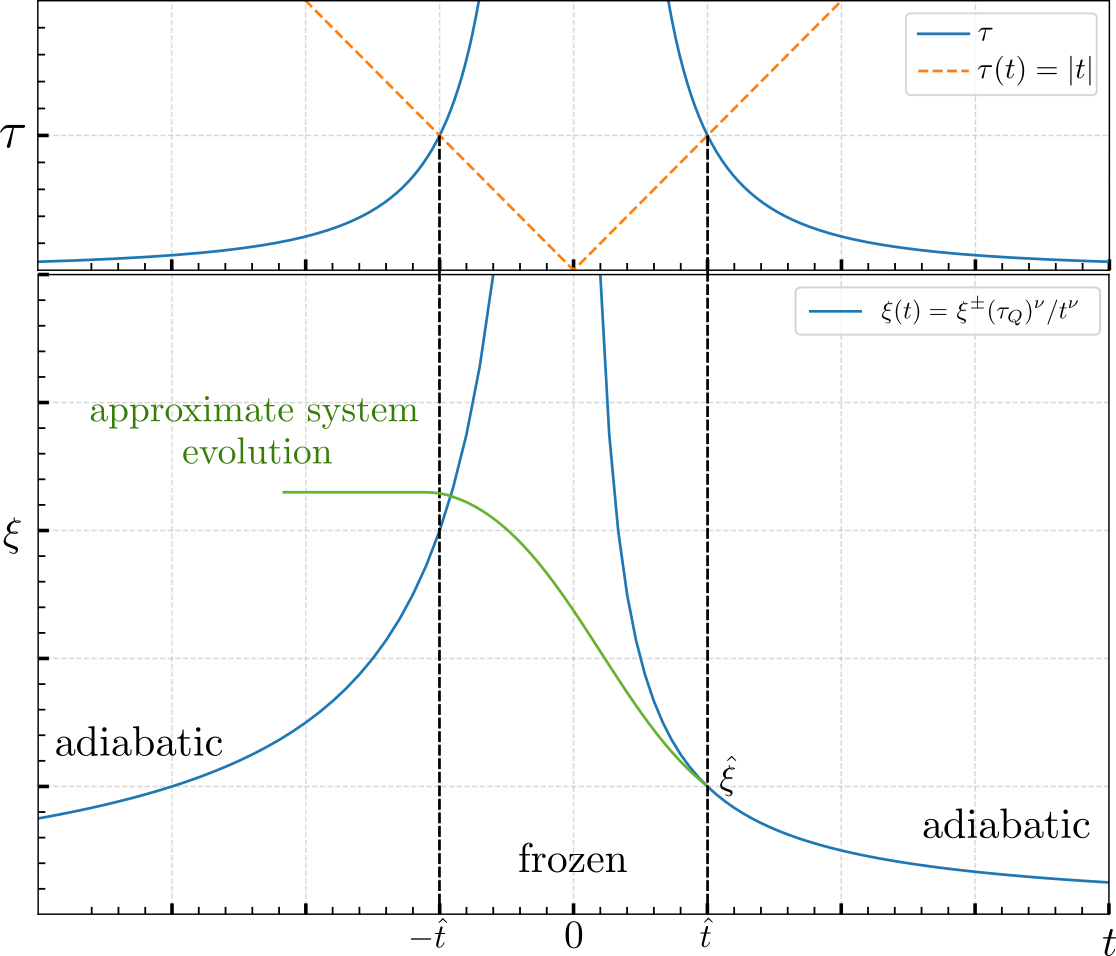
\includegraphics[width=0.7\linewidth]{graphics/KZM-divergences.png}
		\caption{In the top plot the divergence of the relaxation time $\tau$, i.e. the critical slowing down, is shown in blue versus the time $t$ during a linear quench. The freeze-out of the current state happens roughly at $\tau(\hat{t}) =	\hat{t}$, visualized by the intersection with the dotted orange line. In the bottom plot the divergence of the equilibrium $\xi$ on the quench time is shown. Before $\hat{t}$ an initially equilibrated system system evolves approximately adiabatic when quenched, following the blue line. After the freeze-out, the actual correlation diverges from the equilibrium behavior, shown by the sketched green line. Note that in this parameterization, a cooling quench runs from $t > 0$ to $t < 0$. The frozen domain walls are topologically stable in time.}
		\label{Fig::Freezeout}
	\end{figure}
	The system quantities after the quench will be directly related to their equilibrium values at $\hat{t}$. Combining
	\begin{equation}
		\hat{t} =	\varepsilon(\hat{t}) \tau_Q \qquad \text{and} \qquad  \hat{t} =	\tau(\hat{t}) = \tau(\varepsilon(\hat{t})) =	\tau_\varepsilon \big | \varepsilon(\hat{t}) \big |^{-\nu z}
	\end{equation}
	yields the reduced temperature at $\hat{t}$
	\begin{equation}
		\big|\varepsilon (\hat{t}) \big| =	\left(\frac{\tau_\varepsilon}{\tau_Q} \right)^{\frac{1}{1 + \nu z}} ~.
	\end{equation}
	For the scaling of $\xi$ this means
	\begin{equation} \label{Eq::KZM-scaling}
		\xi \propto \hat{\xi} := \xi(\varepsilon(\hat{t})) =	\xi_0 / |\varepsilon(\hat{t})|^{\nu} =	\xi_0 \bigg| \frac{\tau_Q}{\tau_\varepsilon} \bigg |^{\frac{\nu}{1 + \nu z}} ~,
	\end{equation}
	so the frozen value of the correlation length scales with the quench timescale like $\hat{\xi} \propto \tau_Q^{\frac{\nu}{1 + \nu z}}$~.
	The freeze-out of the correlation length implies domains of order with an extent proportional to $\hat{\xi}^2$. The domain walls separating ordered areas may have influences on different properties of the surface, including conductivity, an important quantity for the semiconductor industry. Knowledge of how the defect density on the surface behaves might help to prepare ideal silicon surfaces. \\
	
	It is important to note that the KZM is a statistical phenomenon and will only be able to predict how the frozen correlation lengths will behave on average for many quenches or very large systems. In general the freeze-out correlation length $\hat{\xi}$ as well as the final correlation length will naturally differ from the predicted behavior, at least locally.
	\chapter{Simulating Dynamics} \label{Chapter::Simulating-Dynamics}
	While most numerical studies of phase transitions rely on Monte Carlo techniques \cite{rastelli2004monte, ferrenberg1991critical, hasenbusch2005two}, this work, inspired by Laguana and Zurek \cite{laguna1997density}, focuses on the use of \textbf{stochastic differential equations}. Their mathematical basics and a derivation of a Langevin equation for our case  will be outlined in the following.
	\section{Stochastic Differential and Langevin Equations}
	\subsection{Stochastic Differential Equations}
	Put simply, stochastic differential equations (SDEs) are the stochastic generalizations of common differential equations like
	\begin{equation} \label{Eq::diff-eq}
		y(t + \text{d}t) =	y(t) + A(y(t), t) \mathrm{d}t ~,
	\end{equation}
	with an  infinitesimal time interval $\text{d}t$ and a given function $A(y(t), t)$. Eq.~\eqref{Eq::diff-eq} describes a \textbf{continuous, memoryless, deterministic} process. For every time point $t + \text{d}t$, one can predict the value $y(t+\text{d}t)$ knowing the values $y(t)$ and $\text{d}t$. SDEs describe continuous, memoryless \textbf{stochastic} processes, also called continuous \textbf{Markov processes}. For every time point definite probabilities are assigned to all $y(t + \text{d}t)$. These properties impose strict limitations on a generalization of Eq.~\eqref{Eq::diff-eq}. It turns out that the generalization must be of the form
	\begin{equation} \label{Eq::std-langevin-eq}
		y(t + \text{d}t) =	y(t) + A(y(t), t) \text{d}t + D^{1/2} \left(y(t), t\right) n(t) (\text{d}t)^{1/2}~.
	\end{equation}
	The random variable $n(t)$ is the unit normal random variable  $\mathcal{N}(0,1)(t) \equiv n(t)$. $A(y(t), t)$ and $D(y(t), t)$ are called the \textbf{drift} and \textbf{diffusion} function. Eq.~\eqref{Eq::std-langevin-eq} is called the standard form \textbf{Langevin equation} and it represents an update formula for the continuous Markov process. It is the only way to construct a mathematically self-consistent formulation, meaning that performing one step $\text{d}t$ or two steps $\alpha \text{d}t$ and $(1 - \alpha)\text{d}t$, $\alpha \in (0, 1)$ yields equivalent results. The proof is given in the appendix of \cite{gillespie1996mathematics}. \\
	
	The probability density $P(N)$, for $\mathcal{N}(\mu, \sigma^2)$ with mean $\mu$ and standard deviation $\sigma$ to take on the value $N$, is given by
	\begin{equation}
		P(N) =	\frac{1}{\sqrt{2\pi \sigma^2}} e^{-\frac{(N - \mu)^2}{2\sigma^2}} ~.
	\end{equation}
	Normal random variables satisfy
	\begin{equation}
	 	a + b \mathcal{N}(\mu, \sigma^2) =	\mathcal{N}(a + b\mu, b^2\sigma^2)~.
	\end{equation}
	  To obtain the widely used \textbf{differential }or \textbf{white noise }form of the Langevin equation out of Eq.~\eqref{Eq::std-langevin-eq}, we define the \textbf{Gaussian white noise process} $\Gamma(t)$ by
	\begin{equation}
		\Gamma(t) :=	\lim\limits_{\text{d}t \rightarrow 0} \mathcal{N}(0, 1/\text{d}t) = \lim\limits_{\text{d}t \rightarrow 0} \frac{n(t)}{(\text{d}t)^{1/2}}.
	\end{equation}
	Its expectation values $\langle~\cdot~\rangle$ satisfy
	\begin{equation} \label{Eq::Gauss-dist-property}
		\left \langle \Gamma(t) \right \rangle = 0 \qquad \text{and} \qquad  			\left \langle \Gamma(t) \Gamma(t + t')\right \rangle =	\delta(t') ~.
	\end{equation}
	Rearranging Eq.~\eqref{Eq::std-langevin-eq} to
	\begin{equation}
		\frac{y(t + \text{d}t) - y(t)}{\text{d}t} =	A(y(t), t) + D^{1/2} (y(t), t) \frac{n(t)}{(\text{d}t)^{1/2}} ~,
	\end{equation}
	and taking the limit $\text{d}t \rightarrow 0$ yields the differential form
	\begin{equation} \label{Eq::Differential-Langevin-eq}
		\frac{d}{\text{d}t} y(t) =	A(y(t), t) + D^{1/2}(y(t), t) \Gamma(t)~.
	\end{equation}
	Einstein showed that  $A(y(t), t)$ and $D(y(t), t)$ are not independent if they are supposed to accurately describe a thermodynamic system \cite{einstein1905molekularkinetischen}. Their relation will be subject of the next section.
	
	
	\subsection{Ornstein-Uhlenbeck Process and Brownian Motion} \label{Section::Brownian-Motion}
	\subsubsection{Ornstein-Uhlenbeck process}
	The Ornstein-Uhlenbeck (OU) process is central to the mathematical description of Brownian motion with linear forces. It describes a continuous Markov process with drift and diffusion functions of the form
	\begin{equation}
		A(y(t), t) =	- \frac{1}{\zeta} y(t) \qquad \text{and} \qquad D(y(t), t) =	c~.
	\end{equation}
	The constants $\zeta$ and $c$ are the \textbf{relaxation time} and the \textbf{diffusion constant}. Plugging these functions into Eq.~\eqref{Eq::std-langevin-eq} gives
	\begin{equation}\label{Eq::OU-Langevin}
		y(t + \text{d}t) =	y(t) - \frac{1}{\zeta} y(t) \text{d}t + c^{1/2} n(t) (\text{d}t)^{1/2}~.
	\end{equation}
	The quantity $y(\text{d}t)$ is normally distributed since it is the sum of a constant $y(0) (1 - \frac{\text{d}t}{\zeta})$ and the normal random variable $n(\text{d}t)$. Hence, $y(2dt)$ is normally distributed, being the linear combination of two statistically independent normal random variables $y(\text{d}t)$ and $n(2dt)$. By induction $y(t)$ is normally distributed for all times. Calculating mean and variance of $y(t)$ defines its distribution.
	Using the properties of \autoref{Eq::Gauss-dist-property}, the differential equations for the first and second moment of $y$ are calculated to
	\begin{equation}
		\left \langle y(t + \text{d}t) \right \rangle =	\left \langle y(t) \right \rangle - \frac{1}{\zeta} \left \langle y(t) \right \rangle \text{d}t~,
	\end{equation}
	and
	\begin{equation}
		\left \langle y^2(t + \text{d}t) \right \rangle =	\left \langle y^2(t) \right \rangle - \frac{2}{\zeta} \left \langle y^2(t) \right \rangle \text{d}t  + c \text{ d}t~.
	\end{equation}
	Solving them with the initial condition $y(0) =	y_0$ yields the mean
	\begin{equation}
		\left \langle y(t) \right \rangle =	 y_0 e^{-t/\zeta}
	\end{equation}
	and the variance
	\begin{equation}
		\left \langle y^2(t) \right \rangle - \left \langle y(t) \right \rangle^2 =	\frac{c\zeta}{2} \left(1 - e^{-2t /	\zeta)}\right)
	\end{equation}
	of $y(t)$. This determines the distribution of $y(t)$ to be
	\begin{equation} \label{Eq::OU-Distribution}
		y(t) =	\mathcal{N}\left(y_0 e^{-t/\zeta}, \frac{c\zeta}{2} \left(1 - e^{-2t /	\zeta)}\right)\right) \overset{t \rightarrow \infty}{=} \mathcal{N}\left(0 , \frac{c\zeta}{2}\right) ~.
	\end{equation}
	\subsubsection{Langevin's approach}
	Now consider a particle with mass $m$ and momentum $p$ that is coupled to a reservoir of temperature $T$. Langevin hypothesized \cite{langevin1908theorie} that the interaction with the bath results in a dissipative drag force $- ({\eta}/{m}) p(t)$ proportional to a dampening constant $\eta$ as well as a fluctuating force $F(t)$. By Newton's second law, its equation of motion is given by
	\begin{equation}
		\frac{\text{d}}{\text{\text{d}t}} p(t) =	- \frac{\eta}{m} p(t) + F(t).
	\end{equation}
	This equation is identified with Eq.~\eqref{Eq::OU-Langevin} at $y(t) \equiv p(t)$
	\begin{equation}
		\frac{\text{d}}{\text{\text{d}t}} p(t) =	- \frac{1}{\zeta} p(t) + { c^{1/2}}{} \Gamma(t).
	\end{equation}
	According to Maxwell-Boltzmann statistics, the directional velocity of the particles will be normally distributed around $\mu_v = 0$ with a standard deviation of $\sigma_v^2 =	k_B T /	m$. Using Eq-~\eqref{Eq::Gauss-dist-property}, for the momentum distribution 
	\begin{equation} \label{Eq::Maxwell-Boltzmann}
		p(t\rightarrow \infty) =	\mathcal{N}(0, m k_B T)~
	\end{equation}
	follows. Comparing \def\equationautorefname{Equations}Eq.~\eqref{Eq::OU-Distribution} and \def\equationautorefname{}Eq.~\eqref{Eq::Maxwell-Boltzmann} \def\equationautorefname{Equation}shows that
	\begin{equation}
		\frac{c \zeta}{2} =	m k_B T~, \qquad \quad \text{or equivalently} \qquad \quad c =	{2 k_B T \eta }~.
	\end{equation}
	Hence, the fluctuating force $F(t)$ can be rewritten as
	\begin{equation}
		F(t) =	\sqrt{2 k_B T \eta} \Gamma(t)~,
	\end{equation}
	confirming that drift and diffusion are not independent. This is a simple form of the powerful \textbf{fluctuation-dissipation theorem}. \\
	
	For a particle \textbf{in a potential} $V(x)$ one eventually obtains the equations of motions
	\begin{align} \label{Eq::Langevin-eq-motion-set-x}
		&\frac{\text{d}}{\text{\text{d}t}} x(t) =	\frac{1}{m} p(t) \qquad \text{and}\\
		\label{Eq::Langevin-eq-motion-set-p}
		&\frac{\text{d}}{\text{\text{d}t}} p(t) =	- \frac{\eta}{m} p(t) - \frac{\partial V(x)}{\partial x} + \sqrt{2 k_B T \eta } \Gamma(t) ~.
	\end{align}
	Methods of numerical solution of the Langevin equation will be presented in \autoref{Section::Numerical-methods}. But first the applicability of the Langevin equation for the silicon surface will be verified. \textcolor{red}{Was gibt es jetzt für zusätzliche Komplikationen? (Durch das potential?)}
	\section{Quantum Mechanical Considerations}
	\subsection{Caldeira-Leggett Master Equation}
	The silicon surface is a complex system subject to quantum mechanical interactions between the surface atoms, as well as with the bulk. The bulk is much larger than the surface and acts as a thermal reservoir, engaging with the dimers through lattice excitations. It is not obvious that classical Langevin equations will be valid in this case. Systems that are coupled to an environment are subject of the theory of open quantum systems, which will be used to derive a set of coupled Langevin equations. \\
	
	Consider the \textbf{Caldeira-Leggett model} \cite{caldeira1981influence} for a quantum mechanical particle of mass $m$, moving in a potential $V(\hat{x})$. We can write its \textbf{free Hamiltonian} $\hat{H}_S$ as
	\begin{equation}
		\hat{H}_S =	\frac{1}{2m} \hat{p}^2 + V(\hat{x})~,
	\end{equation}
	with the position and momentum operators $\hat{x}$ and $\hat{p}$. The reservoir, which is the silicon bulk, is modeled as a set of harmonic oscillators with frequencies $\omega_n$. The bath Hamiltonian $\hat{H}_B$ can be written in terms of the bosonic annihilation and creation operators $\hat{b}_n^\dagger$ and $\hat{b}_n$, or in terms of the canonically conjugated position $\hat{x}_n$ and momentum $\hat{p}_n$ operators
	\begin{equation}
		\hat{H}_B =	\sum_n \hbar \omega_n \left(\hat{b}_n^\dagger \hat{b}_n + \frac{1}{2} \right) =	\sum_n \left(\frac{1}{2 m_n} \hat{p}_n^2 + \frac{1}{2} m_n \omega_n^2 \hat{x}_n^2 \right)~.
	\end{equation}
	We assume that $\hat{x}$ is linearly coupled to the $\hat{x}_n$. Positivity of the global Hamiltonian can be ensured by introducing the interaction $\hat{H}_I$ as
	\begin{equation} \label{Eq::pos-interaction}
		\hat{H}_B + \hat{H}_I + \hat{H}_c  =	\sum_n \hbar \omega_n \left(\hat{b}_n^\dagger  +   \frac{\kappa_n}{\sqrt{2 \hbar m_n \omega_n^3}}~\hat{x} \right) \left(\hat{b}_n  + \frac{\kappa_n}{\sqrt{2 \hbar m_n \omega_n^3}}~\hat{x}\right) ~,
	\end{equation}
	with the coupling constants $\kappa_n$.
	Note that strictly speaking, $\hat{b}^{(\dagger)}$ acts on the bath- and $\hat{x}$ on the system Hilbert space. Unity operators on the respective Hilbert spaces that are required to add them up rigorously are omitted. The positivity of Hamiltonian $\eqref{Eq::pos-interaction}$ is given because of the square form of the terms.  Positive Hamiltonians maintain a lower spectral bound, ensuring that unphysical runaway solutions are prohibited.	The interaction Hamiltonian $\hat{H}_I$ is identified as
	\begin{equation}
		\hat{H}_I =	-\hat{x} \otimes \sum_n \kappa_n \sqrt{\frac{\hbar}{2 m_n \omega_n}} \left(\hat{b}_n + \hat{b}_n^\dagger\right) = - \hat{x} \otimes \sum_n \kappa_n \hat{x}_n	 =:	- \hat{x} \otimes \hat{B} ~,
	\end{equation}
	and the \textbf{counter-term} $\hat{H}_c$ is
	\begin{equation} \label{Eq::counter-term}
		\hat{H}_c =	\hat{x}^2 \sum_n \frac{\kappa_n^2}{2 m_n \omega_n^2} ~.
	\end{equation}
	In the following the counter-term is absorbed into $\hat{H}_S$. The Hamiltonian of the combined system is given by
	\begin{equation}
		\hat{H}_{SB} = \hat{H}_S + \hat{H}_B + \hat{H}_I~.
	\end{equation}
	The composite system is visualized for the case of the Si(001) surface in \autoref{Figure::OQS-Silicon}.
	\begin{figure}[tp]
		\centering
		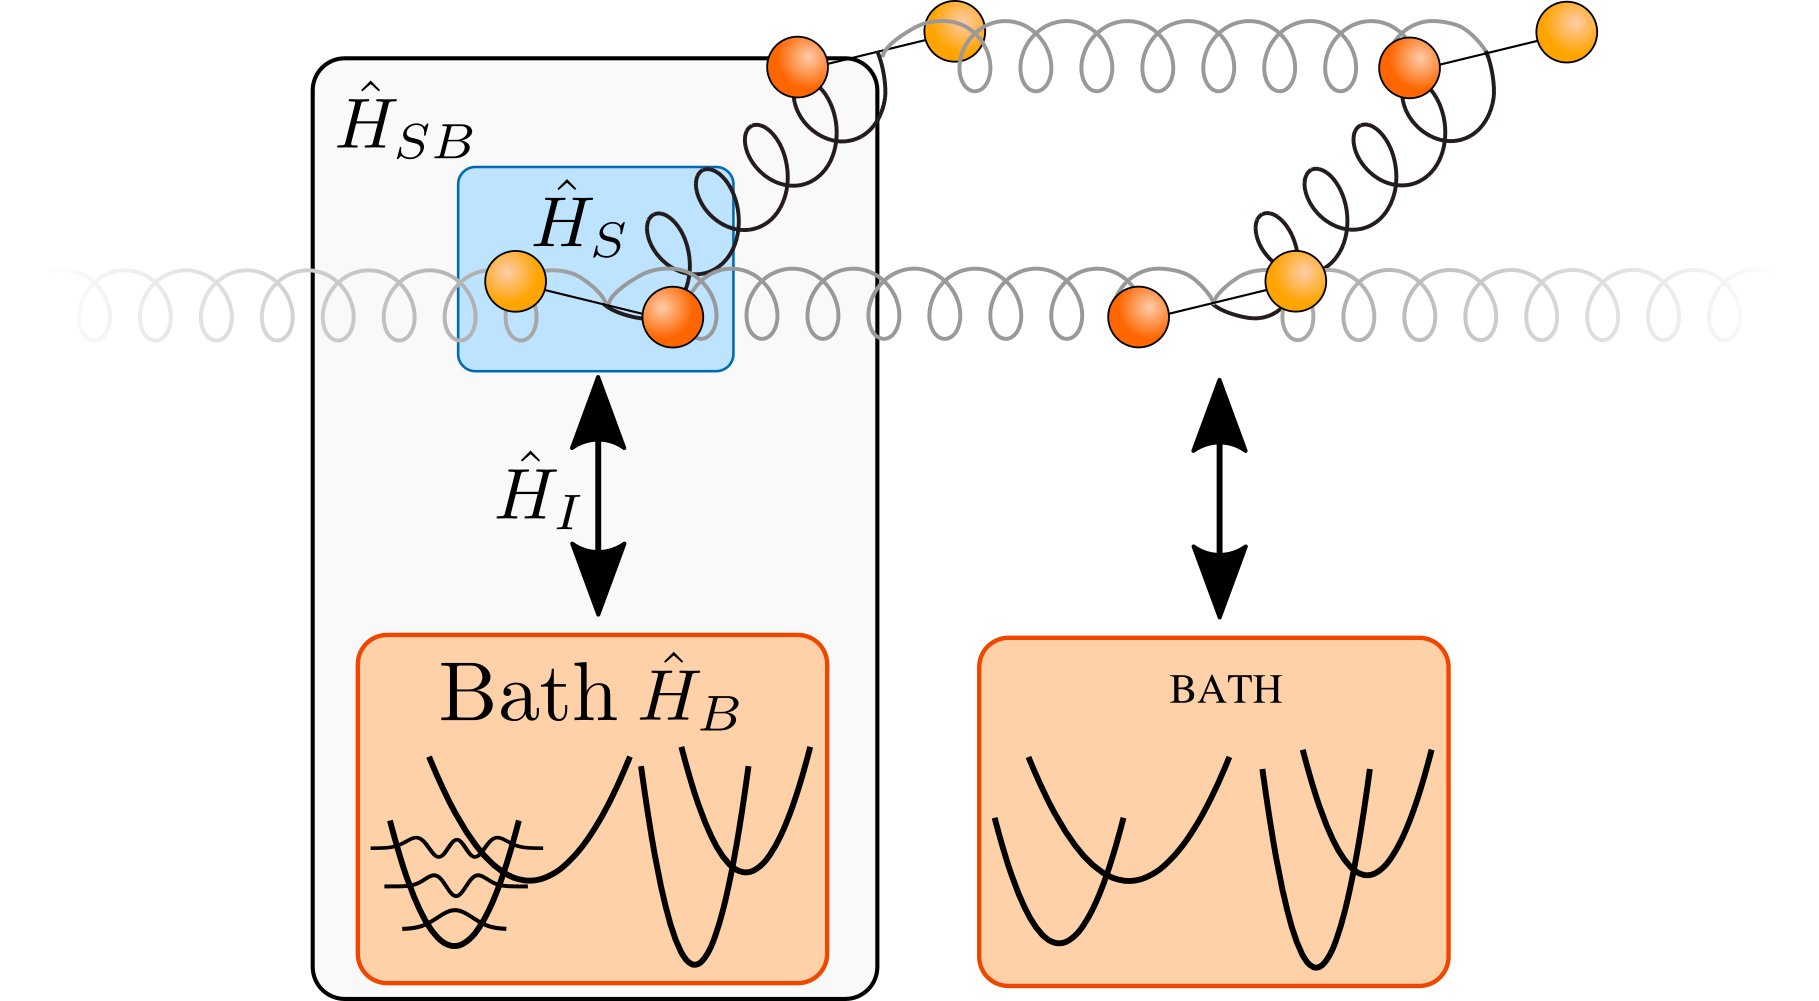
\includegraphics[width=0.8\linewidth]{graphics/OQS-Silicon.png}
		\caption{In the theory of open quantum systems, a system that is thermally coupled to an environment is modeled by a composite Hamiltonian $\hat{H}_{SB} =	\hat{H}_S + \hat{H}_B + \hat{H}_I$. $\hat{H}_S$ denotes the system Hamiltonian describing the potential acting on the dimer. The reservoir is modeled as a set of harmonic oscillators captured in $\hat{H}_B$. The interaction between a dimer and the bath are contained in $\hat{H}_I$. We approximate that every dimer is coupled to a separate bath.}
		\label{Figure::OQS-Silicon}
	\end{figure}
 \\
	
	Since it is neither possible, nor required to solve the dynamics of the whole Hamiltonian, a probabilistic description will be developed. In quantum mechanics this is achieved by modeling the system density matrix $\hat{\rho}_{S}$. In the following, operators in \textbf{interaction picture} are printed \textbf{bold} and $\hbar$ is set to one. The density matrix of the composite system in interaction picture with respect to $\hat{H}_S + \hat{H}_B$ is given by
	\begin{equation}
		\boldsymbol{\hat{\rho}}_{SB} :=	e^{\mathrm{i} \left(\hat{H}_S + \hat{H}_B\right)t} \hat{\rho}_{SB} e^{-\mathrm{i} \left(\hat{H}_S + \hat{H}_B\right)t} ~.
	\end{equation}
	%Starting point is the von Neumann equation for $\boldsymbol{\hat{\rho}}_{SB} :=	e^{\mathrm{i} \left(\hat{H}_S + \hat{H}_B\right)t} \hat{\rho}_{SB} e^{-\mathrm{i} \left(\hat{H}_S + \hat{H}_B\right)t}$ in \textbf{interaction picture} with respect to $\hat{H}_S + \hat{H}_B$:
	 The time evolution of $\boldsymbol{\hat{\rho}}_{SB}$ is
	\begin{equation} \label{Eq::OQS-Startpoint}
		\frac{\partial}{\partial t}\boldsymbol{\hat{\rho}}_{SB}(t) =	- \mathrm{i} \left[\boldsymbol{\hat{H}}_I(t), \boldsymbol{\hat{\rho}}_{SB}(t) \right] ~.
	\end{equation}
	To derive an equation for $\boldsymbol{\hat{\rho}}_S$ the reservoir degrees of freedom are traced out
	\begin{equation} \label{Eq::Tracing-Out-Reservoir}
		\begin{split}
			\frac{\partial}{\partial t} \boldsymbol{\hat{\rho}}_S(t) &=	\text{tr}_B \left \lbrace \frac{\partial}{\partial t} \boldsymbol{\hat{\rho}}_{SB}(t) \right \rbrace =	-\mathrm{i}~\text{tr}_B \left\lbrace \left[\boldsymbol{\hat{H}}_I(t), \boldsymbol{\hat{\rho}}_{SB}(t)\right] \right\rbrace  \\
			&=	-\mathrm{i}~\text{tr}_B \left\lbrace \left[\boldsymbol{\hat{H}}_I(t), {\hat{\rho}}_{SB}(0)\right] \right \rbrace - \int_{0}^{t} \text{d}t'~ \text{tr}_B \left\{  \left[\boldsymbol{\hat{H}}_I(t), \left[\boldsymbol{\hat{H}}_I(t'), \boldsymbol{\hat{\rho}}_{SB}(t') \right]\right]  \right\} \\
			&=- \int_{0}^{t} \text{d}t'~ \text{tr}_B \left\{  \left[\boldsymbol{\hat{H}}_I(t), \left[\boldsymbol{\hat{H}}_I(t'), \boldsymbol{\hat{\rho}}_S(t') \otimes \overline{\rho}_B \right]\right]  \right\}~.
		\end{split}
	\end{equation}
	The second line in Eq.~\eqref{Eq::Tracing-Out-Reservoir} is obtained by integrating Eq.~\eqref{Eq::OQS-Startpoint} and solving for ${\hat{\rho}}_{SB}(0)$. Bath and system are assumed to be in a product state at the initial time ${\hat{\rho}}_{SB}(0) =	\hat{\rho_S}(0) \otimes \overline{\rho}_B$. Therefore the trace
		\begin{equation}
		\text{tr}_B \left\lbrace \left[\boldsymbol{\hat{H}}_I(t), \boldsymbol{\hat{\rho}}_{SB}(0)\right] \right \rbrace =	0
	\end{equation}
	vanishes. The \textbf{Born approximation} assumes that the reservoir density matrix is stationary. In this case, $\boldsymbol{\hat{\rho}}_{SB}(t)$ decomposes to $\boldsymbol{\hat{\rho}}_{SB}(t) = \boldsymbol{\hat{\rho}}_S(t) \otimes \overline{\rho}_B$ for all times and the third line is obtained. The integrand in  Eq.~\eqref{Eq::Tracing-Out-Reservoir} typically decays rather fast (see \autoref{Section::Appendix-Caldeira-Legget}). Hence, the \textbf{Markov approximation} \cite{landi2022nonequilibrium} is applicable. This involves the replacement $\boldsymbol{\hat{\rho}}_S(t') \rightarrow \boldsymbol{\hat{\rho}}_S(t)$, as well as  sending the upper limit of the integral to infinity. Substituting $\tau =t - t'$ yields the \textbf{Redfield-II} master equation
	\begin{equation} \label{Eq::Redfield-II}
		\frac{\partial}{\partial t} \boldsymbol{\hat{\rho}}_S(t) = - \int_{0}^{\infty} \text{d}\tau~ \text{tr}_B \left\{  \left[\boldsymbol{\hat{H}}_I(t), \left[\boldsymbol{\hat{H}}_I(t - \tau), \boldsymbol{\hat{\rho}}_S(t) \otimes \overline{\rho}_B \right]\right]  \right\} ~.
	\end{equation}
	Transforming Eq.~\eqref{Eq::Redfield-II} back to the Schrödinger picture gives
	\begin{equation} \label{Eq::Caldeira-Legget-Startpoint}
		\frac{\partial}{\partial t} {\hat{\rho}}_S(t) =	-\mathrm{i}~\left[\hat{H}_S, \rho_S(t)\right] - \int_{0}^{\infty} \text{d}\tau~ \text{tr}_B \left\{  \left[{\hat{H}}_I, \left[{\boldsymbol{\hat{H}}}_I(- \tau), {\hat{\rho}}_S(t) \otimes \overline{\rho}_B \right]\right]  \right\}~.
	\end{equation}
	The integral in the second term of Eq.~\eqref{Eq::Caldeira-Legget-Startpoint} can be rearranged to
	\begin{equation} \label{Eq::CD-Trace-with-Kernels}
		\int_{0}^{\infty} \text{d}\tau \left(\frac{\mathrm{i}}{2} D(\tau) \Big[\hat{x}, \big\{\boldsymbol{\hat{x}}(-\tau), \hat{\rho}_S(t)\big\} \Big] - \frac{1}{2} D_1(\tau) \Big[\hat{x}, \big[\boldsymbol{\hat{x}}(-\tau) , \hat{\rho}_S(t)\big]\Big]\right)~,
	\end{equation}
	with the noise kernel $D_1(\tau)$ and dissipation kernel $D(\tau)$ defined as in \autoref{Section::Appendix-Caldeira-Legget}. The noise and dissipation kernels disappear on the timescale of the relaxation $\tau_B$ of the reservoir. When doing the Markov approximation, it is assumed that this timescale is much shorter than the relaxation time of the system $\tau_S$. This is used again by approximating $\boldsymbol{\hat{x}}(-\tau)$ by its free dynamics
	\begin{equation}\label{Eq::free-dynamics}
		\boldsymbol{\hat{x}}(-\tau) =	\hat{x} - \hat{p} \tau~.
	\end{equation}
	For large $\tau > \tau_B$ the integrand decays quickly and for $\tau < \tau_B < \tau_S$, Eq. \eqref{Eq::free-dynamics} is valid in good approximation. Plugging the free dynamics into Eq.~\eqref{Eq::CD-Trace-with-Kernels} allows for the evaluation of the integrals (see \autoref{Section::Appendix-Caldeira-Legget}). This eventually yields the \textbf{Caldeira-Leggett master equation}
	\begin{equation} \label{Eq::Caldeira-Leggett-Master-equation}
		\frac{\text{d}}{\text{d}t} \rho_S(t) =	\underbrace{-\mathrm{i}\left[\hat{H}_S, \rho_S(t) \right]}_{\text{free dynamics}} - \underbrace{\mathrm{i} \eta \Big [\hat{x}, \big\{\hat{p}, \rho_S(t)\big\}\Big ]}_\text{dissipative term} - \underbrace{2 \eta k_B T \Big [\hat{x}, \big[\hat{x}, \rho_S(t)\big]\Big ]}_\text{thermal fluctuations}~.
	\end{equation}
	The damping constant $\eta$ enters the calculation through the parametrization of the spectral density function of the reservoir. The first term in the Caldeira-Leggett master equation describes the free dynamics of the system and resembles the form of the \textbf{von-Neumann} equation. The second term is the dissipative part proportional to the damping constant $\eta$. The thermal fluctuations of the reservoir are captured in the third term proportional to the temperature $T$. The state of the reservoir $\overline{\rho}_B$ follows the \textbf{Bose-Einstein distribution} and determines $T$.
	\subsubsection{Thermalization}
	Investigating the position space representation of Eq.~\eqref{Eq::Caldeira-Leggett-Master-equation} shows that its stationary solution is found to be the position space density matrix
	\begin{equation} \label{Eq::quantum-equilibrium-dist}
		\hat{\rho}_S (x, x') = \frac{1}{Z}	e^{- \beta {V((x + x') /2)}} e^{-\frac{1}{2\beta} (x - x')^2}
	\end{equation}
	with the normalization
	\begin{equation}
		Z =	\int_{-\infty}^{\infty} \text{d}x e^{- \beta {V(x)}}~.
	\end{equation}
	The inverse temperature is again denoted by $\beta =	1 /	k_B T$. The diagonal terms of Eq.~\eqref{Eq::quantum-equilibrium-dist} are identified with the canonical distribution of statistical mechanics. The off-diagonals decay exponentially and vanish for large temperatures. Thus, systems described by Eq.~\eqref{Eq::Caldeira-Leggett-Master-equation} thermalize in the sense that their steady state solution is analogue to the canonical distribution. 
	\subsection{Equations of Motion}
	From Eq.~\eqref{Eq::Caldeira-Leggett-Master-equation} one can derive equations of motion for arbitrary observables via
	\begin{equation}\label{Eq::QM-Eq-of-motion}
		\frac{\text{d}}{\text{d}t} \left \langle \hat{A} \right \rangle =	\text{tr} \left\{\hat{A} \frac{\text{d}}{\text{d}t } \hat{\rho}_S(t)\right\}~,
	\end{equation}
	using the invariance of the trace under cyclic permutations. Comparing the results of Eq.~\eqref{Eq::QM-Eq-of-motion} for $\hat{x}, \hat{p}$ and $\hat{p}^2$ to the equations of Brownian motion of \autoref{Section::Brownian-Motion}
	\begin{multicols}{2}
		\noindent
		\begin{align*}
			\begin{split}
				&\frac{\text{d}}{\text{d}t} \left \langle \hat{x} \right \rangle =	\frac{1}{m} \left\langle \hat{p} \right \rangle~,
			\end{split}
			\\
			\begin{split}
				&\frac{\text{d}}{\text{d}t} \left \langle \hat{p} \right \rangle = - 	\left\langle  \frac{\partial V(\hat{x})}{\partial \hat{x}} \right \rangle - \eta \left \langle \hat{p} \right \rangle ~,
			\end{split}
			\\
			\begin{split}
				&\frac{\text{d}}{\text{d}t} \left \langle \hat{p}^2 \right \rangle =	- \left\langle \hat{p} \frac{\partial V(\hat{x})}{\partial \hat{x}} + \frac{\partial V(\hat{x})}{\partial \hat{x}} \hat{p} \right \rangle \\
				&\qquad \qquad ~- 2 \eta \left \langle \hat{p}^2 \right \rangle + 2 \eta k_B T ~,
			\end{split}
		\end{align*}
		\begin{align*}
			\begin{split}
				&\frac{\text{d}}{\text{d}t} \left \langle {x}(t) \right \rangle  =	~\frac{1}{m} \left \langle {p}(t) \right \rangle ~,
			\end{split}
			\\
			\begin{split}
				&\frac{\text{d}}{\text{d}t} \left \langle {p}(t) \right \rangle =	- 	\left \langle \frac{\partial V({x})}{\partial {x}} \right \rangle - \eta \left \langle {p}(t) \right \rangle ~,
			\end{split}
			\\
			\begin{split}
				&\frac{\text{d}}{\text{d}t} \left \langle {p}^2(t) \right \rangle = - \left\langle 2 {p}(t) \frac{\partial V({x})}{\partial {x}}\right \rangle \\
				&\qquad \qquad \quad ~ - 2 \eta \left \langle {p}^2(t) \right \rangle + 2 \eta k_B T~.
			\end{split}
		\end{align*}
	\end{multicols}
	shows that the two equation sets share the same structure.		
%	\begin{table}[h]
%		\centering
%		\caption{Version2.2. The equations of motion for  $\hat{x}, \hat{p}$ and $\hat{p}^2$ calculated from  Eq.~\eqref{Eq::QM-Eq-of-motion} are compared to Brownian motion of \autoref{Section::Brownian-Motion}. It is evident that the structure of equations of motion for the quantum expectation values matches the expectation values from Brownian motion. Therefore the quantum mechanical case is called \textbf{Quantum Brownian Motion}.}
%		\renewcommand{\arraystretch}{1.7}
%		\begin{tabular}{c l l}
%			\toprule
%			Quantity & Quantum Brownian Motion $\qquad$  & Brownian Motion \\
%			\midrule
%			$x$ & $\frac{\text{d}}{\text{d}t} \left \langle \hat{x} \right \rangle \hspace{3pt}=	\frac{1}{m} \left\langle \hat{p} \right \rangle$ & $\frac{\text{d}}{\text{d}t} \left \langle {x}(t) \right \rangle \hspace{3pt}  =	~\frac{1}{m} \langle {p}(t) \rangle $ \\
%			$p$ & $\frac{\text{d}}{\text{d}t} \left \langle \hat{p} \right \rangle ~= - 	\left\langle  \frac{\partial V(\hat{x})}{\partial \hat{x}} \right \rangle - \eta \left \langle \hat{p} \right \rangle$ &	$\frac{\text{d}}{\text{d}t} \left \langle {p}(t) \right \rangle ~=	- 	\left \langle \frac{\partial V({x})}{\partial {x}} \right \rangle - \eta \left \langle {p}(t) \right \rangle$ \\
%			$p^2$ & \makecell[l]{$\frac{\text{d}}{\text{d}t} \left \langle \hat{p}^2 \right \rangle =	- \left\langle \hat{p} \frac{\partial V(\hat{x})}{\partial \hat{x}} + \frac{\partial V(\hat{x})}{\partial \hat{x}} \hat{p} \right \rangle$ \\ $ \qquad \qquad \hspace{2pt} - 2 \eta \left \langle {p}^2(t) \right \rangle + 2 \eta k_B T$} & \makecell[l]{$\frac{\text{d}}{\text{d}t} \left \langle {p}^2(t) \right \rangle = - \left\langle 2 {p}(t) \frac{\partial V({x})}{\partial {x}}\right \rangle $ \\ $ \qquad \qquad \hspace{3pt} \quad - 2 \eta \left \langle {p}^2(t) \right \rangle + 2 \eta k_B T$}\\
%			\bottomrule
%		\end{tabular}
%		\label{Table::QBM-vs-BM}
%	\end{table} \renewcommand{\arraystretch}{1.2}
%	
%	\textcolor{red}{Version 2:}\\
%	The results of Eq.~\eqref{Eq::QM-Eq-of-motion} for $\hat{x}, \hat{p}$ and $\hat{p}^2$ are compared to the equations of Brownian motion of \autoref{Section::Brownian-Motion} in \autoref{Table::QBM-vs-BM}. The two equation sets share the same structure. \\	
	Especially interesting is the last term in the equations for $\langle \hat{p}^2 \rangle$. This is the diffusion constant in the case of Brownian motion and it matches the quantum mechanical term. Hence, it is possible to derive the diffusion constant from microscopic considerations. We conclude that the classical equations of motion Eq.~\eqref{Eq::Langevin-eq-motion-set-x} and Eq.~\eqref{Eq::Langevin-eq-motion-set-p} are the classical correspondence to the equations of $\langle \hat{x} \rangle$ and $\langle \hat{p} \rangle$. In the following, the classical equations of motion are used to describe the silicon surface. Since the silicon dimers interact, the potential $V(x) =	V(x, {x_i})$ is a function of the coordinates $x_i$ of the other dimers, leading to a \textbf{coupling} between the differential equations. Additionally, $V(x, {x_i})$ is \textbf{nonlinear} in $x$, eventually yielding a coupled set of nonlinear stochastic differential equations. An analytic solution is impossible and therefore we turn to numerical solutions in the next section.
	\section{Numerical Methods and Molecular Dynamics} \label{Section::Numerical-methods}
	The update-form Eq.~\eqref{Eq::std-langevin-eq} of the Langevin equation is very useful for its numerical solution. A simple method of solution is the straight implementation of Eq.~\eqref{Eq::std-langevin-eq}, which is called the \textbf{Euler-Maruyama method} \cite{kloeden1992stochastic}. Practically, a system of first-order stochastic differential equations
	\begin{align}
		&x(t + \text{d}t) = x(t)	+ \frac{1}{m} p(t) \text{d}t ~, \\
		&p(t + \text{d}t) =	p(t) - \frac{\eta}{m} p(t) \text{d}t - \frac{\partial V(x(t))}{\partial x} \text{d}t + \sqrt{2 k_B T \eta} ~ n(t) \sqrt{\text{d}t} ~,
	\end{align}
	is solved. The Euler-Maruyama method is straightforward to implement and computationally inexpensive, but shows discretization artifacts even for small step sizes $\text{d}t$. Since the integration of the equations of motion usually takes much less time than the evaluation of $V(x(t))$ \cite{frenkel2023understanding}, many efforts have been made to improve the weak convergence \cite{kloeden1992stochastic} of integration schemes. \\
	
	The topic of simulating microscopical systems by numerically solving Newton's equations of motion is called \textbf{molecular dynamics}. Molecular dynamics is widely used in biophysics, chemical physics but also material sciences. When Langevin equations are employed to simulate thermally open systems, one also talks about \textbf{Langevin dynamics}. Larini et al. \cite{larini2007langevin} compare some of the common numerical integration schemes for Langevin equations. They show that in general the popular Brunger-Brooks-Karplus (BBK) \cite{brunger1984stochastic} scheme is robust method with good accuracy and numerical efficiency. It integrates in three steps \cite{izaguirre2001langevin}, half a kick
	\begin{equation}
		p\left(t + \tfrac{1}{2} \text{d}t \right) =	\left(1 - \tfrac{1}{2} \eta \text{d}t \right) p(t) - \tfrac{1}{2} \text{d}t \tfrac{\partial V(x(t))}{\partial x} + \tfrac{1}{2} \sqrt{2\eta{k_B T}} n(t) \sqrt{\text{d}t}~,
	\end{equation}
	drift
	\begin{equation}
		x(t + \text{d}t) = x(t) +  p\left(t + \tfrac{1}{2} \text{d}t\right) \text{d}t~,
	\end{equation}
	and half a kick
	\begin{equation}
		p\left(t\right) =	\left(1 + \tfrac{\text{d}t}{2} \eta \right)^{-1} \left( p\left(t + \tfrac{\text{d}t}{2}\right) - \tfrac{1}{2} \text{d}t \tfrac{\partial V(x(t + \text{d}t))}{\partial x} + \tfrac{1}{2} \sqrt{2\eta{k_B T}} n({t + \text{d}t}) \sqrt{\text{d}t} \right) ~.
	\end{equation}
	%	\begin{align}
		% 		\nonumber \\
		%		&p_i\left(t + \tfrac{1}{2} dt \right) =	\left(1 - \tfrac{1}{2} \eta dt \right) p_i(t) - \tfrac{1}{2} dt \tfrac{\partial V(x_i(t), \{x\})}{\partial x_i} + \tfrac{1}{2} \sqrt{2\eta{k_B T}} n_i(t) \sqrt{dt}~, \nonumber \\
		%		&\text{drift} \nonumber \\
		%		&x_i(t + dt) = x_i(t) +  p_i\left(t + \tfrac{1}{2} dt\right) dt~, 		\label{Eq::BBK-method} \\
		%		&\text{half a kick} \nonumber \\
		%		&p_i\left(t\right) =	\left(1 + \tfrac{dt}{2} \eta \right)^{-1} \left( p_i\left(t + \tfrac{dt}{2}\right) - \tfrac{1}{2} dt \tfrac{\partial V(x_i(t + dt), \{x\})}{\partial x_i} + \tfrac{1}{2} \sqrt{2\eta{k_B T}} n_i({t + dt}) \sqrt{dt} \right)\nonumber.
		%	\end{align}
	Compared to higher-order schemes, like the fourth-order Hamiltonian Runge-Kutta scheme \cite{press2002numerical}, that require multiple potential evaluations, the BBK method is faster with limited loss of accuracy \cite{larini2007langevin}. The BBK integration step is slightly slower than the one of Euler-Maruyama but it makes up through its much greater stability regarding larger step sizes. This ultimately results in significantly faster simulation speeds. The stability of the schemes is briefly compared in \autoref{Section::Benchmarks}. \\
	
	The theoretical foundation for the simulation of the Si(001) surface using Langevin equations is now established. The following section will deal with the modeling of the several times mentioned potential.
	\section{The Model}
	\subsection{The Ising model} \label{Section::Ising-Model}		
	Since the Ising model has discrete states, it is not suitable for continuous modeling with equations of motion. However, the Ising model is well known and has been used several times \cite{brand2023dimer, pillay2004revisit, ihm1983structural, schaller2023sequential} to study the Si(001) surface and can serve as a limiting case. Brand et al. \cite{brand2023critical} found good agreement between the Si(001) phase transition and the Ising critical exponents.  Their results are relevant for the following investigations and therefore the Ising model will be shortly discussed below. \\
	
	The two dimensional Ising model describes spins $\sigma_{i ,j} =	\pm 1$ on a lattice. Consider the anisotropic case without external field. Its nearest-neighbor Hamiltonian is given by
	\begin{equation} \label{Eq::Ising-Hamiltonian}
		H =	- \sum_{i,j}^{} \left(J_\parallel \sigma_{i ,j} \sigma_{i ,j + 1} + J_\perp \sigma_{i, j} \sigma_{i +1 ,j} \right) ~,
	\end{equation}
	with $J_{\delta}$, $\delta \in \{\parallel, \perp\}$, being the effective nearest-neighbor coupling strengths. The two dimensional anisotropic Ising model is analytically solvable \cite{onsager1944crystal} and exhibits a continuous phase transition at
	\begin{equation} \label{Eq::Crit-Temp-Ising}
		\sinh \left( \frac{2 |J_\parallel|}{k_B T_c} \right) \sinh \left( \frac{2 |J_\perp|}{k_B T_c}\right) =	1.
	\end{equation}
	The equilibrium correlation lengths for $T > T_c$ can be determined from the coupling constants \cite{mccoy1973two} by
	\begin{equation} \label{Eq::Ising-Corrlength-Coupling}
		\frac{\xi_\delta(T)}{a_\delta} =	\left(\ln \left[ \coth \left(\frac{|J_\delta|}{k_B T}\right)\right] - \frac{2 |J_{\overline{\delta}}|}{k_B T}\right)^{-1} ~,
	\end{equation}
	with $a_\delta$ being the lattice spacing in $\delta$ direction and $\overline{\delta}$ marking the direction perpendicular to $\delta$. \\
	
	To describe the silicon surface with the Ising model, the equilibrium positions of the silicon dimers in \autoref{Fig::dimer-configs} (b) are mapped to the Ising spin values $\sigma_{i ,j} =	\pm 1$. In theoretical works, density functional theory (DFT) calculations are often employed to calculate configuration energies.   Eq.~\eqref{Eq::Ising-Hamiltonian} can then be used to fit effective  $J_\delta$ to the DFT results. In experiments, the correlation lengths $\xi_\delta$ can be measured and used to extract $J_\delta$ through Eq.~\eqref{Eq::Ising-Corrlength-Coupling}. Calculating quantitative values for $J_\delta$ can reveal important information about the nature of the microscopic interactions (between the dimers), especially if Eq.~\eqref{Eq::Ising-Hamiltonian} is extended to next-nearest neighbor couplings or even further. Additionally, theoretical
%	\begin{wrapfigure}[17]{r}{0.35\textwidth}
%		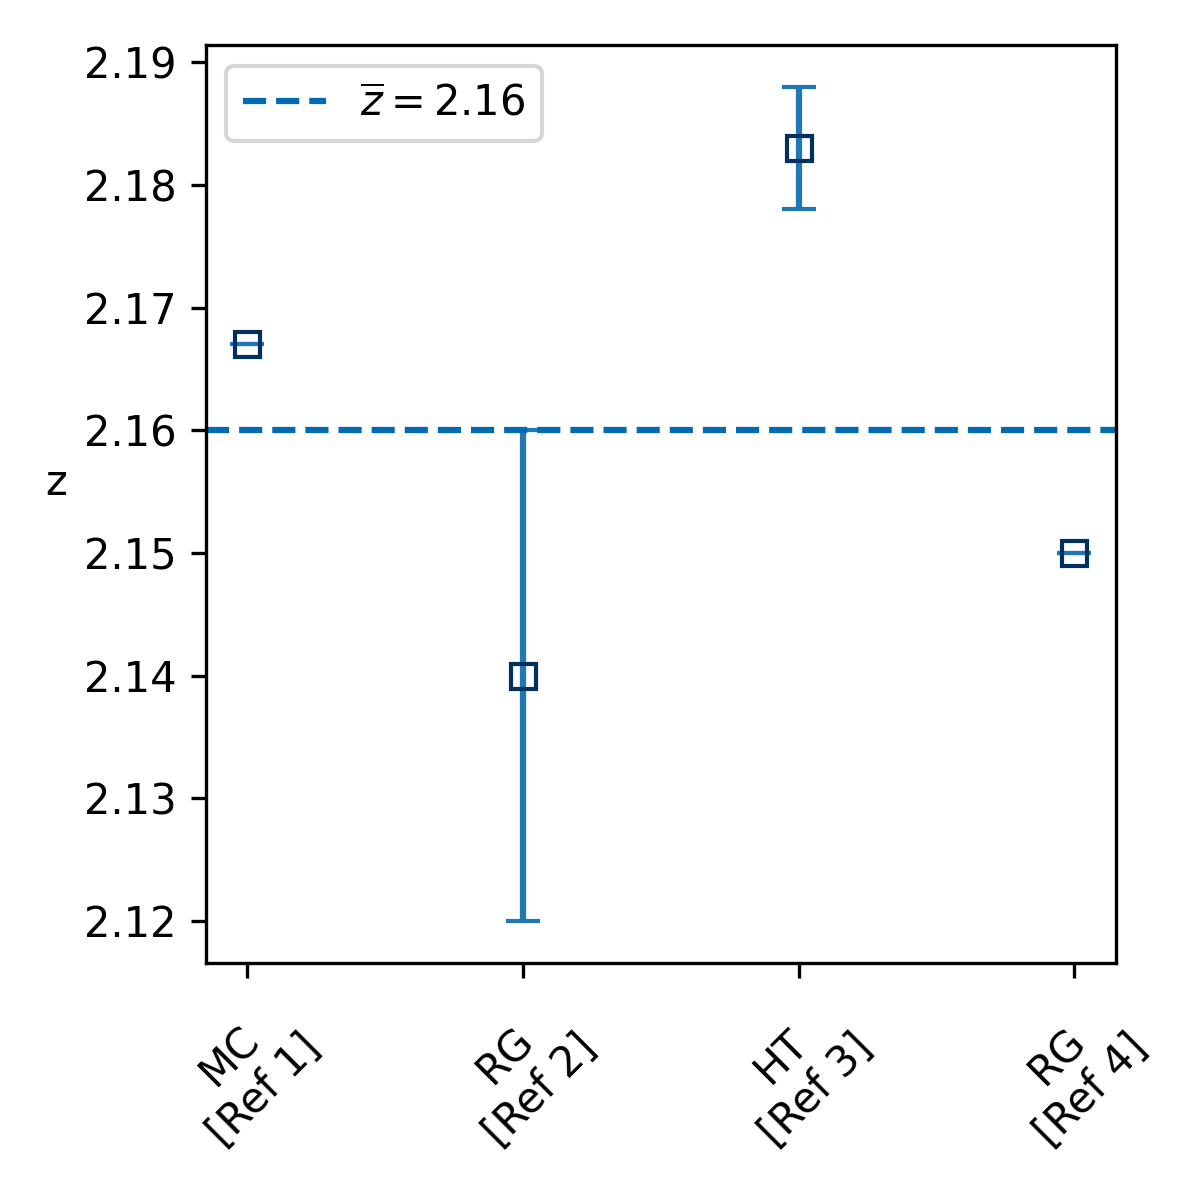
\includegraphics[width=\linewidth]{graphics/z-values}
%		\caption{Recent results for the dynamic critical exponent $z$ are summarized. The datapoints are obtained by Monte-Carlo methods (MC) \cite{nightingale2000monte}, renormalization group calculations (RG) \cite{adzhemyan2022dynamic, duclut2017frequency} and high-temperature expansion (HT) \cite{dammann1993dynamical}.}
%		\label{Figure::Ising-z-values}
%	\end{wrapfigure}
	results of the Ising model can be used to analyze the surface further. Eq.~\eqref{Eq::Crit-Temp-Ising} may be used to estimate the transition temperature. Eventually, a simple theoretical model of the Si(001) system is obtained which also may be used in
	\begin{wraptable}[15]{r}{0.4\textwidth}
		\caption{Recent results for the dynamic critical exponent $z$ are summarized. The estimates are obtained by Monte-Carlo methods (MC) \cite{nightingale2000monte}, renormalization group calculations (RG) \cite{adzhemyan2022dynamic, duclut2017frequency} and high-temperature expansion (HT) \cite{dammann1993dynamical}.}
		\renewcommand{\arraystretch}{1.3}
		\begin{tabular}{c c l}
			Source & Method  & Result \\
			\midrule
			\cite{nightingale2000monte} & MC &  $2.167$ \\
			\cite{adzhemyan2022dynamic} & RG &  $2.14 \pm 0.02$ \\
			\cite{duclut2017frequency} & RG &  $2.183 \pm 0.005$ \\
			\cite{dammann1993dynamical} & HT &  $2.15$ \\
			\bottomrule
			Average &  &  $2.16$ \\
		\end{tabular}
		\label{Figure::Ising-z-values}
	\end{wraptable}
	computer simulations. \\
	
	The Ising model gives name to its universality class. It is characterized by a continuous phase transition with a scalar order parameter and $\mathbb{Z}_2$ symmetry. The static critical exponents of the Ising universality class can be calculated analytically \cite{cardy1996scaling}. For $\nu$ the exact value
	\begin{equation}
		\nu =	1
	\end{equation}
	is obtained. As noted in \autoref{Section::Dynamic-Scaling}, the anisotropic Ising model is part of Model A of critical dynamics \cite{hohenberg1977theory}. The constant $c$ of Eq.~\eqref{Eq::Model-A-z} has been estimated by numerous method. Some recent results for $z$ are shown in \autoref{Figure::Ising-z-values}. \\
	%An overview of the relevant critical exponents is given in \autoref{Table::Ising-crit-expo}.
	%	\begin{table}[hb]
		%		\centering
		%		\begin{tabular}{c c c}
			%			$\qquad \nu \qquad$ & z & $ \quad ~ \tfrac{\nu}{1 + \nu z} ~ \quad$ \\
			%			1 & $2.1667 \pm 0.0005$ & $0.3158 \pm ?$ \\
			%		\end{tabular}
		%		\caption{The static critical exponents of the Ising universality class can be calculated analytically \cite{cardy1996scaling}. The value for $z$ is the estimate of Nightingale et al. \cite{nightingale2000monte}, who used MC techniques.}
		%		\label{Table::Ising-crit-expo}
		%	\end{table}
	\subsection{The Classical XY Model}
	The classical XY model and the Ising model can be viewed as two special cases of the Potts model \cite{potts1952some}. It generalizes the Ising model to allow $q$, instead of two, states. The states are uniformly distributed on a circle as shown in \autoref{Fig::States} (a). In the limit $q \rightarrow \infty$ the XY model is obtained. It allows continuous states on the unit circle and is thus suitable to be described by Langevin equations. \\
	
	The two dimensional XY Hamiltonian with nearest-neighbor interactions is given by
	\begin{equation} \label{Eq::XY-isotropic}
		\begin{split}
			H =&- \sum_{i,j}^{} \left(J_\parallel \vec{s}_{i,j} \vec{s}_{i,j + 1} + J_\perp  \vec{s}_{i,j} \vec{s}_{i + 1,j} \right)   \\
			=&- \sum_{i,j}^{} \left(J_\parallel  \cos \left(\vartheta_{i,j} - \vartheta_{i, j+1} \right) + J_\perp  \cos \left(\vartheta_{i,j} - \vartheta_{i+1, j} \right) \right)	 ~,
		\end{split}
	\end{equation}
	with unit-length vectors
	\begin{equation}
		\vec{s}_{i, j} =	\left(\begin{array}{c}
			\cos \vartheta_{i, j} \\
			\sin \vartheta_{i, j}
		\end{array}\right) ~,
	\end{equation}
	characterizing the state of the lattice site. These rotors are defined by a continuous angle $\vartheta$ on the interval $[0, 2\pi)$. Although the exact solution of the two dimensional XY model is intractable, Mattis \cite{mattis1984transfer} used a transfer matrix approach to approximate an analogue to Eq.~\eqref{Eq::Crit-Temp-Ising}. He arrived at
	\begin{equation} \label{Eq::Crit-Temp-XY}
		\frac{2 k_B T_c}{|J_\parallel|} \ln \left(\frac{2 k_B T_c}{|J_\perp|}\right) =	1 ~, 
	\end{equation}
	with $J_\parallel \geq J_\perp$. The relation between the coupling constants and the equilibrium correlation lengths is not known at the moment. For low temperatures, the XY model undergoes a transition to a quasi ordered phase of bound vortex-antivortex pairs. A comparison between the phase diagram resulting from this equation and Eq.~\eqref{Eq::Crit-Temp-Ising} is shown in \autoref{Fig::XY-Ising-PD}.\\
	\begin{figure}
		\centering
		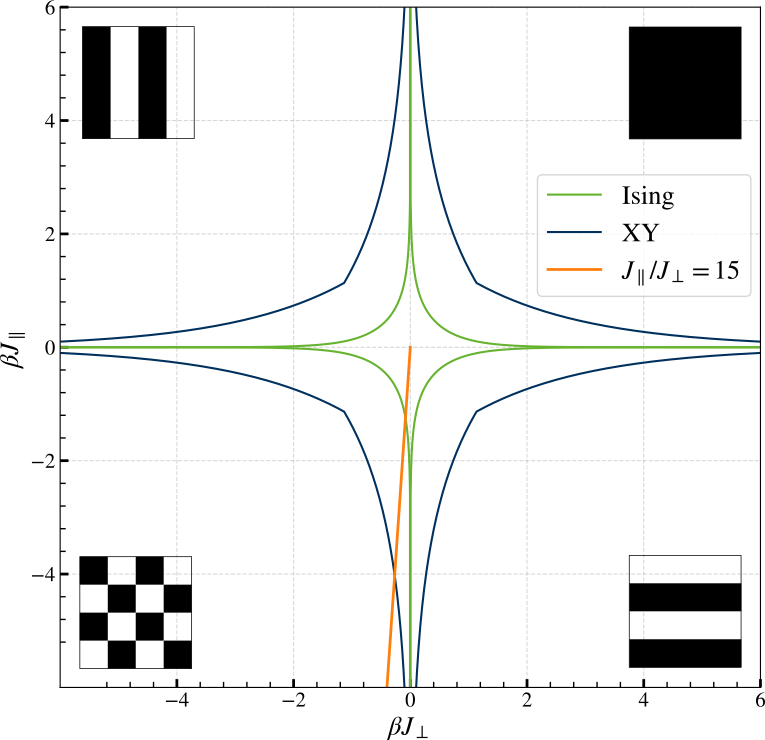
\includegraphics[width=0.8\linewidth]{graphics/Phase-diagram-Ising-XY-clean.png}
		\caption{The phase diagram of the Ising model and the isotropic XY model is shown in the $\beta J_\parallel-\beta J_\perp-$plane. The green and blue lines determine the phase boundary between the unordered and ordered state of the Ising and the XY model respectively. The unordered high-temperature phase is found in the center for $\beta J_\delta \rightarrow 0$. Depictions of the Ising model ordering are shown in the corners of the diagram. They visualize whether neighbors are correlated or anti-correlated. The ordered state in the XY case is a quasi ordered phase of bound vortex-antivortex pairs, which looks a bit different. The neighbor correlations are however the same as in the Ising case. The area of high temperature phase of the XY model is larger than in the Ising model, indicating that larger coupling constants are needed to introduce ordering. The orange line shows an equipotential line with $J_\parallel /	J_\perp =	15$ for both coupling constants smaller than zero. A system that is Quenched according as described in \autoref{Section::Quench} for a fixed $J_\parallel /	J_\perp$ follows this line from the center outwards.}
		\label{Fig::XY-Ising-PD}
	\end{figure}
	
	The two dimensional XY model does not exhibit a phase transition in the conventional sense. The \textbf{Mermin-Wagner theorem} \cite{mermin1966absence} prohibits the breaking of its continuous $\text{O}(2)$ symmetry through short-range interactions. Instead, the system shows the \textbf{Kosterlitz-Thouless transition} (KT transition) \cite{JMKosterlitz_1973, berezinskii1971destruction}. The usual power laws are not applicable to this transition because the correlation length diverges exponentially at the critical point. Hence, the two dimensional XY model does not belong to any universality class. \\
	
	We can add a $p$-fold symmetry breaking field of strength $h$ to the XY Hamiltonian
	\begin{equation} \label{Eq::XY-Hamilton-Field}
		H =- \sum_{i,j}^{} \left(J_\parallel  \cos \left(\vartheta_{i,j} - \vartheta_{i, j+1} \right) + J_\perp  \cos \left(\vartheta_{i,j} - \vartheta_{i+1, j} \right) \right)	+ h \sum_{i,j} \cos(p\vartheta_{i,j}) ~,
	\end{equation}
	explicitly breaking the $\text{O}(2)$ symmetry. Such fields may very well be experimentally realized by crystalline anisotropies. We will in the following differentiate between the Hamiltonians \eqref{Eq::XY-isotropic} and \eqref{Eq::XY-Hamilton-Field} by calling the former \textbf{isotropic} XY model and the latter \textbf{symmetry-broken} or \textbf{anisotropic} XY model. Note that (an-)isotropic here references the plane of the spin rotor and it is not to be confused with the lattice anisotropy of the interactions. \\
	
	The Migdal lattice recursion scheme \cite{migdal1975phase} implies that for $T \rightarrow 0$, the field $h$ is a relevant variable in the sense of \autoref{Section::RG}. The perturbations caused by $h$ will grow as $T$ shrinks, eventually forcing the system into a state of broken symmetry in which one of the directions $\vartheta =	{2 \pi n }/{p}, n \in \left[0, p-1\right]$ is preferred. Hence, any $h$ will lead to deviations in critical behavior from the KT transition. José and Kadanoff \cite{jose1977renormalization} found that this symmetry broken XY model exhibits a continuous phase transition with the critical exponents of a $p$-state Potts model. This results in Ising critical behavior in the case of $p=2$. Hence, the two dimensional XY model with twofold symmetry breaking field is well suited to explore the dynamics of the Si(001) surface.
	\begin{figure}[htp]
		\centering
		\begin{subfigure}{\textwidth}
			\centering
			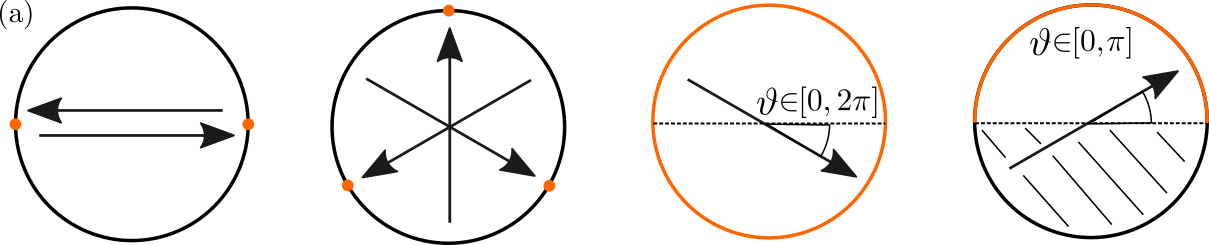
\includegraphics[width=0.9\linewidth]{graphics/Allowed-States.png}
		\end{subfigure} \\
		\par\bigskip % force a bit of vertical whitespace
		\begin{subfigure}{\textwidth}
			\centering
			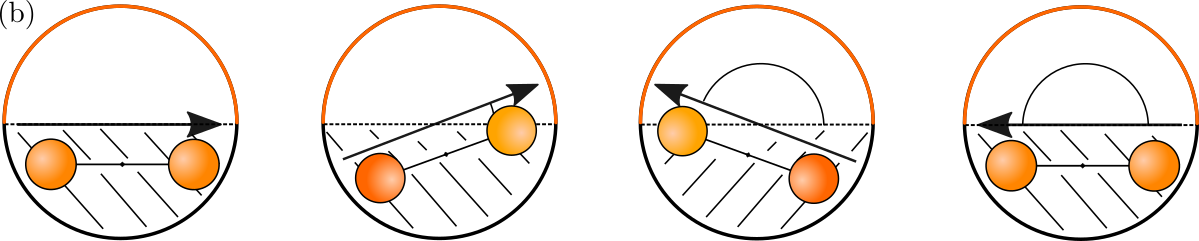
\includegraphics[width=0.9\linewidth]{graphics/State-Mapping.png}
		\end{subfigure}
		\caption{Unit circles are shown as visualizations of the state space. The orange parts are the allowed states. The states are depicted as arrows inside the unit circle. \textbf{(a)} shows the $q$-state Potts model. From left to right: The two-state Potts model, or the Ising model, allows only two points on the unit circle.  The three-state Potts model allows three different spin directions, visualized by the arrows. In the limit $q \rightarrow \infty$ the XY model is obtained. The state is characterized by a continuous angle $\vartheta$. The rightmost circle visualizes the adaptation of the XY model to the silicon surface. Here, only half the circle is allowed. \textbf{(b)} The buckling angles of the silicon dimers are mapped to the rotors of the XY model. Since the silicon atoms are indistinguishable, a rotation by $\pi$ maps to the same state. Hence, the state space is only half the unit circle. Note that the left and right vectors are the same state and strictly speaking one of them can be excluded by defining $\vartheta \in [0, \pi)$.}
		\label{Fig::States}
	\end{figure}
	\subsection{Adaptation to the Si(001) Surface}\label{Sec::XY-to-Silicon}	
	In the following the XY model will be adapted to optimally resemble the silicon surface. \\ 	%In the following some customization steps will be shown to adapt the XY model in a way to optimally resemble the experimentally observed properties of the silicon surface. 
	
	Like done with the Ising model, the aim is to map the position of the dimer to a model state. The natural choice is to identify the dimer buckling angle with the rotor angle $\vartheta$ of the XY model. Since the silicon atoms are indistinguishable, a rotation by $\pi$ translates into the same state. Hence, only $\vartheta \in [0, \pi)$ define unique states, restricting the state space of the XY model. The resulting half circle is shown in the rightmost picture of \autoref{Fig::States} (a). For computational reasons, $\vartheta $ will be shifted by $-\tfrac{\pi}{2}$, eventually yielding $\vartheta \in \left[-\tfrac{\pi}{2}, \tfrac{\pi}{2}\right)$. The restriction is achieved by adding a factor $m=2$ into the interaction terms 
	\begin{equation} \label{Eq::m-introduction}
		J_\delta \cos \left(m \Delta \vartheta_{i, j}\right)~.
	\end{equation}
	The equilibrium position of the dimers is majorly influenced by the location of the minima of the symmetry breaking field. The experimental systems shows two stable buckling angles of about $\pm 20^\circ$. Therefore the symmetry breaking field will be constructed to have two minima on the interval $\left[-\tfrac{\pi}{2}, \tfrac{\pi}{2}\right)$ at the desired angles. The minima satisfy
	%Since the silicon dimers do not have a distinguished direction in contrary to the spin vectors of the XY model, we define the right dimer to point along the arrow \autoref{Fig::DimerMapping}. Additionally, a flip of the pointer by $\pm \pi$ results in the same state, effectively cutting the state space in half. Measuring from the (001) axis (\autoref{Fig::SiliconDiamond}), the angles will be restricted to $\vartheta \in \left[-\tfrac{\pi}{2}, \tfrac{\pi}{2}\right]$.	This is achieved by adding a factor $m = 2$ into the $J_\delta \cos \left(m \Delta \vartheta_{i, j}\right)$ terms. As stated in \autoref{Section::Silicon}, the dimers are buckled by  $18^{\circ}$ corresponding to a an angle $\vartheta^\pm=	\pm 72^\circ \approx	\pm \tfrac{2}{5} \pi $~. The equilibrium positions of Eq.~\eqref{Eq::XY-Hamilton-Field} are determined by the symmetry breaking field and the parameter $p$ since the interaction is $O(2)$-symmetric. The minima satisfy
	\begin{equation}
		\cos \left(p \vartheta^\pm\right) =	-1~,
	\end{equation}
	implying that roughly $ p \approx 2.5$. The final resting position of the dimer is shifted by the repulsive interaction of the dimers. This is covered in \autoref{Section::quantitative}. The movement of the dimers can be approximated to take place in a double well potential \cite{dabrowski1992self}. This is realized by the symmetry breaking shown in \autoref{Fig::XY-Silicon-Potential}. The question arises if the system still belongs to the Ising universality class if $p$ is a rational number and the allowed states are restricted. This will be subject of \autoref{Section::static-scaling}. \\
	
	%to ensure to reproduce the experimental equilibrium positions. The resulting potential of the symmetry breaking field is shown in \autoref{Fig::XY-Silicon-Potential}. \\
	\begin{figure}[thb]
		\centering
		\includegraphics[width=0.8\linewidth]{graphics/XY-Silicon-potential2.png}
		%\caption{The external field in combination with the restriction of $\vartheta$ leads to  the shown potential. The angle is measured from the $(110)$ axis for illustration purposes. The Dynamics of the dimers for sufficiently low temperatures will take place around $\vartheta =	0$, the bucklings of $\vartheta =	\pm \tfrac{1}{2} \pi$ will almost never be reached.}
		\caption{The symmetry breaking field $h$ is shown in blue on the dimer angle. The dimer states are defined on $\vartheta \in [-\tfrac{\pi}{2}, \tfrac{\pi}{2}]$, therefore $h$ repeats after a period of $\pi$. The location of the potential minima are chosen to be located at the according position of the experimental dimers. The red area around $\vartheta =	0$, corresponding to vertical dimers, is strongly suppressed and rarely realized. The dynamics take place in the double well potential shown on the left and on the right of the plot. Note that the two double well potentials are actually located at the same position since the state space is periodic. Some dimer states are depicted at their according angle.}
		\label{Fig::XY-Silicon-Potential}
	\end{figure}
	A suitable order parameter for this model is
	\begin{equation} \label{Eq::Si-Order-Param}
		M_L =	\frac{1}{L^2} \sum_{i,j} m(\vartheta_{i, j}) \qquad \text{with} \qquad	m(\vartheta) =	\sin \left(\tfrac{p}{2} \vartheta\right) ~,
	\end{equation}
	as the $m(\vartheta)$ have maxima at $\vartheta^{+}$ and minima at $\vartheta^{-}$, satisfying $m(\vartheta^+) =	- m (\vartheta^-)$.
	
	The XY model's natural conjugated coordinate is the angle $\vartheta$ and therefore Eq.~\eqref{Eq::Langevin-eq-motion-set-x} and Eq.~\eqref{Eq::Langevin-eq-motion-set-p} have to be adapted to rotary motion. The velocity is replaced by the angular velocity $\omega$ in this case.
	
	Eq.~\eqref{Eq::XY-Hamilton-Field} yields the force
	\begin{equation} \label{Eq::Potential-Derivative}
		\begin{split}
			\frac{\partial V(\{\vartheta\})}{\partial \vartheta_{i, j}} = ~~~& J_\parallel m \Big( \sin \left(\vartheta_{i,j} - \vartheta_{i + 1, j} \right) +   \sin \left(\vartheta_{i,j} - \vartheta_{i-1, j} \right) \Big)	 \\
			+ &J_\perp m \Big( \sin \left(\vartheta_{i,j} - \vartheta_{i, j+1} \right) +  \sin \left(\vartheta_{i,j} - \vartheta_{i, j-1} \right) \Big) \\
			+ &h p \sin(p\vartheta_i)~.
		\end{split}
	\end{equation}
	Eventually, the Langevin equations become
	\begin{align}
		&\frac{\text{d}}{\text{d}t} \vartheta_{i,j}(t) =	 \omega_{i,j}(t)~, \label{Eq::Si-Langevin-theta} \\
		&\frac{\text{d}}{\text{d}t} \omega_{i,j}(t) =	- \frac{\eta}{I} \omega_{i,j}(t) - \frac{1}{I}\frac{\partial V(\{\vartheta\})}{\partial \vartheta_{i,j}} + \sqrt{\frac{2 k_B T \eta}{I^2}} \Gamma(t)~, \label{Eq::Si-Langevin-omega}
	\end{align}
	with the moment of inertia $I$ replacing the mass $m$. The implementation of the integration of this coupled set of stochastic differential equations will be the subject of the next section.
	%	\begin{equation}
		%		\ddot{\vartheta}_{i, j} =	- \frac{\eta}{I} \dot{\vartheta}_{i, j} - \frac{1}{I} V_{i,j}' + \sqrt{\frac{2 k_B T \eta}{I^2}} \Gamma_{i,j}
		%	\end{equation}
	\chapter{Implementation and Results} \label{Chapter::Implementation-Results}
	To reduce finite size corrections it is desirable to consider as large systems as possible. Combined with the critical slowing down described in  \autoref{Section::Dynamic-Scaling}, the task at hand requires an significant computational effort. On top of this comes the stochastic nature of the system. Many realizations have to be simulated to calculate ensemble averages. Additionally, minimizing discretization errors and ensuring convergence when integrating \eqref{Eq::Si-Langevin-omega} forces the choice of a small step size $\text{d}t$. This makes an efficient and fast implementation a crucial part of our investigations.
	\section{GPU Programming}
	Besides the difficulties just described, there is an advantage that can be made use of. The Langevin equations for the different lattice sites may be coupled, but the integration step to $t + \text{d}t$ only depends on the $\vartheta_{i, j}(t)$ of the previous step. Hence, the integrations can be performed simultaneously in real time. This allows parallelization of the computation, making the problem ideal for a graphical processing unit (GPU) implementation. \\
	
	The main difference between a conventional single core implementation on a central processing unit (CPU) and one on GPU is the number of processing cores involved. One core can execute one  instruction at a time. While CPUs only have few ($\sim 10$) powerful processing cores, GPUs are made up of up to $\sim 10^4$ cores. The CPU traditionally solves problems in a sequential matter, doing calculation after calculation. This makes them suitable for use cases where the next step directly depends on the one before. In contrast, the GPU is able to perform many independent calculations real time simultaneously on its different cores. In situations where this is applicable, GPU implementations yield a significant speedup of up to a factor of $100$ \cite{che2008performance}. A concept of the different solution approaches is shown in \autoref{Fig::CPU-vs-GPU}.\\
	\begin{figure}[htp]
		\centering
		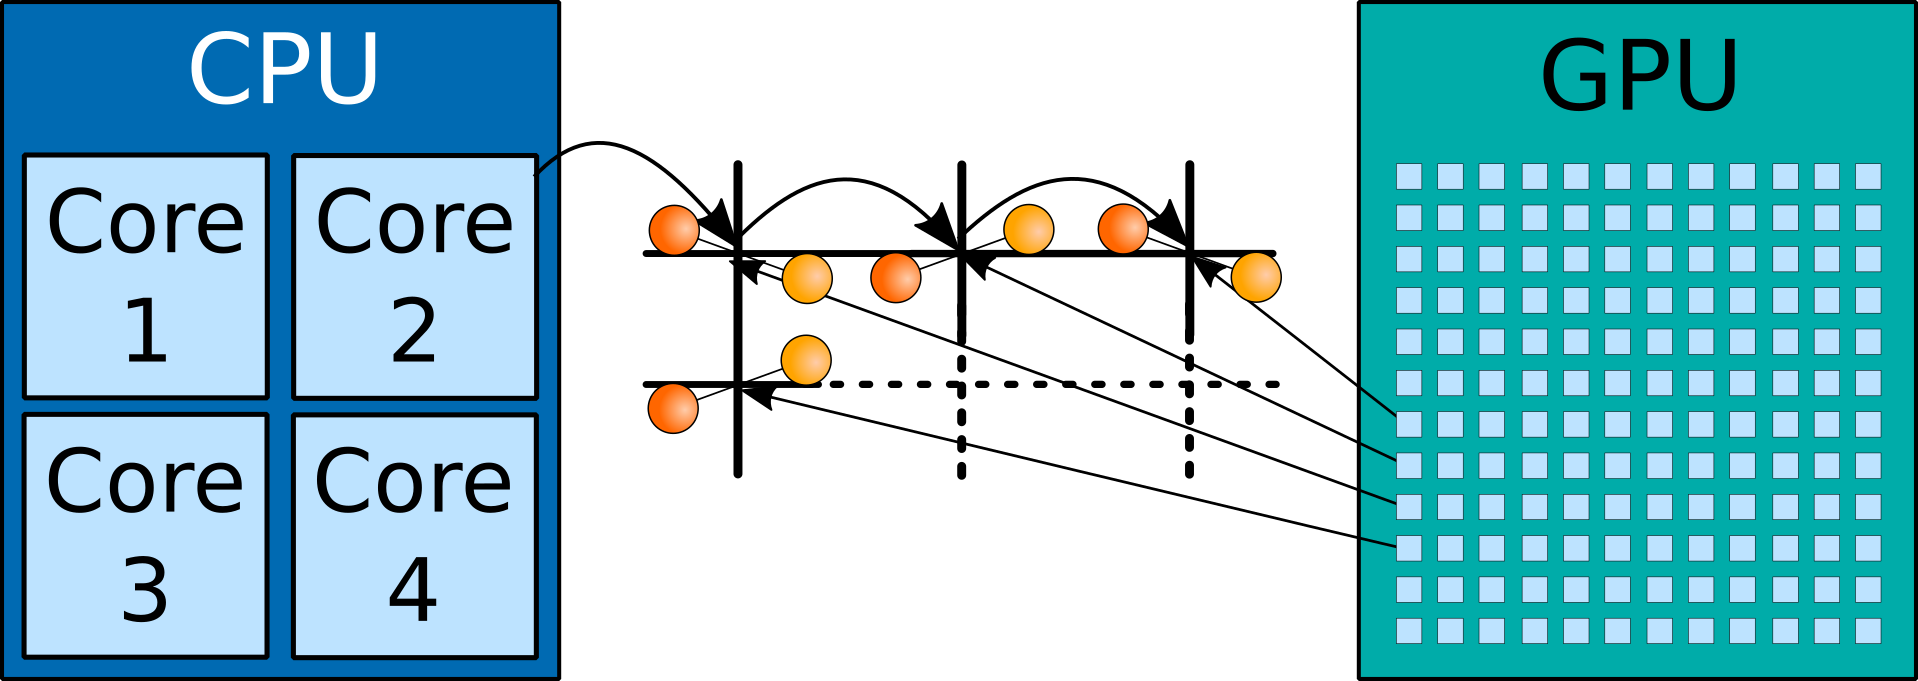
\includegraphics[width=0.8\linewidth]{graphics/CPU-vs-GPU-2.png}
		\caption{The conceptual structures of CPUs and GPUs are shown. A CPU usually consists of less than $10$ cores, while a current GPU is made up of more than $10^3$ cores. The center depicts a lattice. A CPU using single core processing would integrate the Langevin equation for lattice site $i$ and move on to site $i+1$. The use of multi core processing would allow the shown CPU to integrate four sites simultaneously. In contrast, using GPU programming enables to evaluate the Langevin equation at about $10^3 - 10^4$ sites at the same time.}
		\label{Fig::CPU-vs-GPU}
	\end{figure}
	
	The simulation is implemented in CUDA C\texttt{++} \cite{cuda} using Thrust \cite{thrust} as high level interface. Inspired by Ahnert et al.'s work \cite{ahnert2014solving}, the architecture has been extended to accommodate stochastic differential equations. The random numbers are generated using CUDA's built in library cuRAND. Refer to \autoref{Table::Hardware-Software} for details on the hardware and software employed.
	
	\section{Dimensional Analysis} \label{Section::quantitative}
	\subsubsection{Units in the simulation}
	The numerical implementation of Eq.~\eqref{Eq::Si-Langevin-theta} and \eqref{Eq::Si-Langevin-omega} naturally uses dimensionless numbers. To assign physical meaning to the numbers, all quantities are expressed in multiples of a shared scale. Selecting the moment of inertia $I$ as energy scale eliminates its three appearances in \eqref{Eq::Si-Langevin-omega}. Natural units with $\hbar =	c =	1$ are used in the following. \\
	
	The dimensionless angular velocity $\Omega$ in units of $I$ is
	\begin{equation}
		\Omega(t) =	I\omega(t)~.
	\end{equation}
	The dimensionless version of Eq.~\eqref{Eq::Si-Langevin-omega} becomes
	\begin{equation} \label{Eq::Dimensionless-Omega}
		\begin{split}
			\Omega_{i,j}(t + \text{d}t) &=	\Omega(t) - \eta \Omega_{i,j}(t) \frac{\text{d}t}{I} - {I}\frac{\partial V(\{\vartheta\})}{\partial \vartheta_{i,j}} \frac{\text{d}t}{I} + \sqrt{\frac{2 T \eta}{I^2}} n(t) I \sqrt{\text{d}t} \\
			&=	\Omega(t) - \eta \Omega_{i,j}(t) \text{d}\sigma - \frac{\partial v(\{\vartheta\})}{\partial \vartheta_{i,j}} \text{d}\sigma + \sqrt{{2 \kappa \eta}} n(t) \sqrt{\text{d}\sigma}~,
		\end{split}
	\end{equation}
	with the dimensionless time, potential and temperature
	\begin{align}
		&\sigma =	t /	I, \\
		&v(\vartheta) =	I V(\vartheta), \qquad \text{and} \\
		&\kappa =	IT.
	\end{align}
	The dimensionless coupling constants are denoted by
	\begin{equation} \label{Eq::dimensionless-coupling}
		j_\delta =	IJ_\delta \qquad \text{and} \qquad \rho = I h~.
	\end{equation}
	The second line of Eq.~\eqref{Eq::Dimensionless-Omega} will be used in the simulation. The equation of motion \eqref{Eq::Si-Langevin-theta} of the dimensionless buckling angle $\vartheta$ 
	\begin{equation}
		\begin{split}
			\vartheta(t + \text{d}t) &=	\vartheta(t) + \Omega(t) \text{d}\sigma =	\vartheta(t) + I \omega(t) \frac{\text{d}t}{I} \\
			&= \vartheta(t) + \omega(t) \text{d}t
		\end{split}
	\end{equation}
	is invariant of the chosen energy scale. The moment of inertia of a silicon dimer is approximated as two point masses $m_{Si} \approx 28u =	26 \text{ GeV}$ with a distance of $2r \approx 2 ~\text{\AA} \approx 10~ \text{keV}^{-1}$, yielding
	\begin{equation}
		I \approx 2m_{Si} r^2 \approx	2 \left(26 ~\text{GeV}\right) \left(5 ~\text{keV}^{-1}\right)^2 =	1300 \text{ meV}^{-1}~.
	\end{equation}
	 In a high temperature state, the dimers flip between the two potential minima about once per $10 \text{ ps}$ \cite{dabrowski1992self}. The used step size should be much smaller than this. For $\text{d}t =	1 \text{ ps}$, a dimensionless step size of
	\begin{equation}
		\text{d} \sigma =	\text{d}t / I \approx \frac{1.5 \text{meV}^{-1}}{1300 \text{meV}^{-1}} \approx 0.001
	\end{equation}
	would be required. However, we will base the actual step size on the observed discretization error in \autoref{Section::Benchmarks}. 
	\subsubsection{Quantitative experimental values}
%	The dimensionless critical temperature has a value of
%	\begin{equation}
%		\kappa_c =	1300 \text{ meV}^{-1} \cdot 16.43 \text{ meV} \approx 22100~,
%	\end{equation}
	Brand et. al determine the experimental critical temperature to $190.6 \text{ K}$, or  
	\begin{equation} \label{Eq::Exp-Tc}
		T_c =	16.43 \text{ meV.}
	\end{equation} 
	They furthermore extracted the correlation lengths and used \eqref{Eq::Ising-Corrlength-Coupling} to fit the Ising model coupling constants $J_\delta^{\text{Ising}}$ to the experiment. They obtain
	\begin{equation} \label{Eq::Exp-coupling-ising}
		J_\parallel^{\text{Ising}} =	-24.9 \text{ meV} 	\qquad \text{and} \qquad 	J_\perp^{\text{Ising}} =	-0.8 \text{ meV},
	\end{equation}
	and a ratio of $J_\parallel^{\text{Ising}} /	J_\perp^{\text{Ising}} \approx	31$.
	 Assuming this ratio for the XY model, Eq.~\eqref{Eq::Crit-Temp-XY} can be employed to estimate $J_\delta^{\text{XY}}$. The obtained couplings
	\begin{equation}
		J_\parallel^{\text{XY}} = 82.46 \text{ meV}\qquad \text{and} \qquad J_\perp^\text{XY} =	2.66 \text{ meV} ~,
	\end{equation}
	are larger than the Ising values, which is expected \cite{aizenman1980comparison}. %corresponding to the dimensionless values $j_\delta =	I J_\delta$ of
%	\begin{equation} \label{Eq::Parameter-guess}
%		j_\perp =	3580 \qquad \text{and} \qquad j_\parallel =	110980~.
%	\end{equation}
	The effective critical temperature is
	\begin{equation} \label{Eq::Tc-XY-31}
		T_c /	J_\parallel^{\text{XY}} =	0.19899~.
	\end{equation}
	The effective critical temperature $T_c^{\text{XY}} /	J_\parallel$ of the isotropic XY solely depends on the ratio$J_\parallel /	J_\perp$. An expression can be derived by rewriting Eq.~\eqref{Eq::Crit-Temp-XY} as
	\begin{equation}
		\frac{2 T_c}{|J_\perp|} \ln \left(\frac{2 T_c}{ |J_\perp|}\right) =	\frac{|J_\parallel|}{|J_\perp|}~.
	\end{equation}
	This equation has the structure of
	\begin{equation}
		x \ln (x) =	a,
	\end{equation}
	which is solved by
	\begin{equation}
		x =	e^{W_0 (a)}~,
	\end{equation}
	with the principal branch $W_0$ of the Lambert $W$ function. Resubstituting $x$ and using the identity
	\begin{equation}
		e^{W_0(x)} =	\frac{x}{W_0(x)} ~,
	\end{equation} 
	yields
	\begin{equation} \label{Eq::XY-crit-general-effective}
		{T^{\text{XY}}_c} /	{J_\parallel} =	\frac{1}{2 W_0 \left(\frac{J_\parallel}{J_\perp}\right)}~.
	\end{equation}
 	The symmetry breaking field $h$ is expected to increase the critical temperature of the system. José et. al \cite{jose1977renormalization} determined the qualitative relation between $h$ and $T_c$ by a renormalization group calculation for the anisotropic XY model with integer $p$. It is therefore anticipated that the couplings of the symmetry broken model are located between the Ising and XY values.
	
	\subsubsection{Fitting the coupling constants to DFT calculations}
	Numerous investigations calculated configuration energies of the Si(001) \cite{fu2001molecular, ramstad1995theoretical} surface by density functional theory (DFT) methods and fitted the Ising model parameters accordingly \cite{pillay2004revisit, inoue1994order, ihm1983structural, xiao2019spontaneous}. Their calculations will be used in the following to obtain approximate values for the symmetry broken XY model.  \\
	
	The model in use has four parameters that influence the configuration energy. These are the interaction couplings $J_\parallel, J_\perp$, and the field parameters $h$ and $p$. Previous DFT calculations come to the result that that the equilibrium buckling angle doesn't change significantly in the different surface configurations. We will approximate \cite{pillay2004revisit, brand2023critical}
	\begin{equation}
		\vartheta \approx 72^\circ,
	\end{equation}
	for all reconstructions. DFT calculations determine energy differences so that $n$ configurations can be used to determine $n-1$ variables. Additionally, diagonal interactions $J_\times$ will be added to correctly describe the surface energies. Considering the geometries of \autoref{Figure::surface-configurations}, we can write down the the total surface energy per dimer. The surface energy consists of the inter-dimer interaction as well as their potential energy. Periodic boundary conditions are used. For the reconstructions $c(4 \times 2), p(2 \times 2), p(2 \times 1)$ and $p(4\times1)$, the equations
	\begin{equation}
		\begin{split}
			\cos(4\vartheta)&J_\parallel&+& \cos(4\vartheta)&J_\perp &+ &2J_\times &+ \cos \left(\vartheta p\right) h &=~&	E_0, \\
			\cos(4\vartheta)&J_\parallel&+& &J_\perp &+ &2J_\times \cos(4 \vartheta) &+ \cos \left(\vartheta p\right) h &=~&	E_0 + E_{p(2\times 2)}, \\
			&J_\parallel&+& &J_\perp &+ &2J_\times &+ \cos \left(\vartheta p\right) h &=~&	E_0 + E_{p(2\times 1)}, \\
			&J_\parallel&+&\cos\left(4\vartheta \right)&J_\perp &+ &2J_\times \cos(4 \vartheta) &+ \cos \left(\vartheta p\right) h &=~&	E_0 + E_{p(4\times 1)},
		\end{split}
	\end{equation}
	are obtained from Eq. \eqref{Eq::XY-Hamilton-Field}. Subtracting $E_0$ yields
	\begin{figure}[tb]
		\centering
		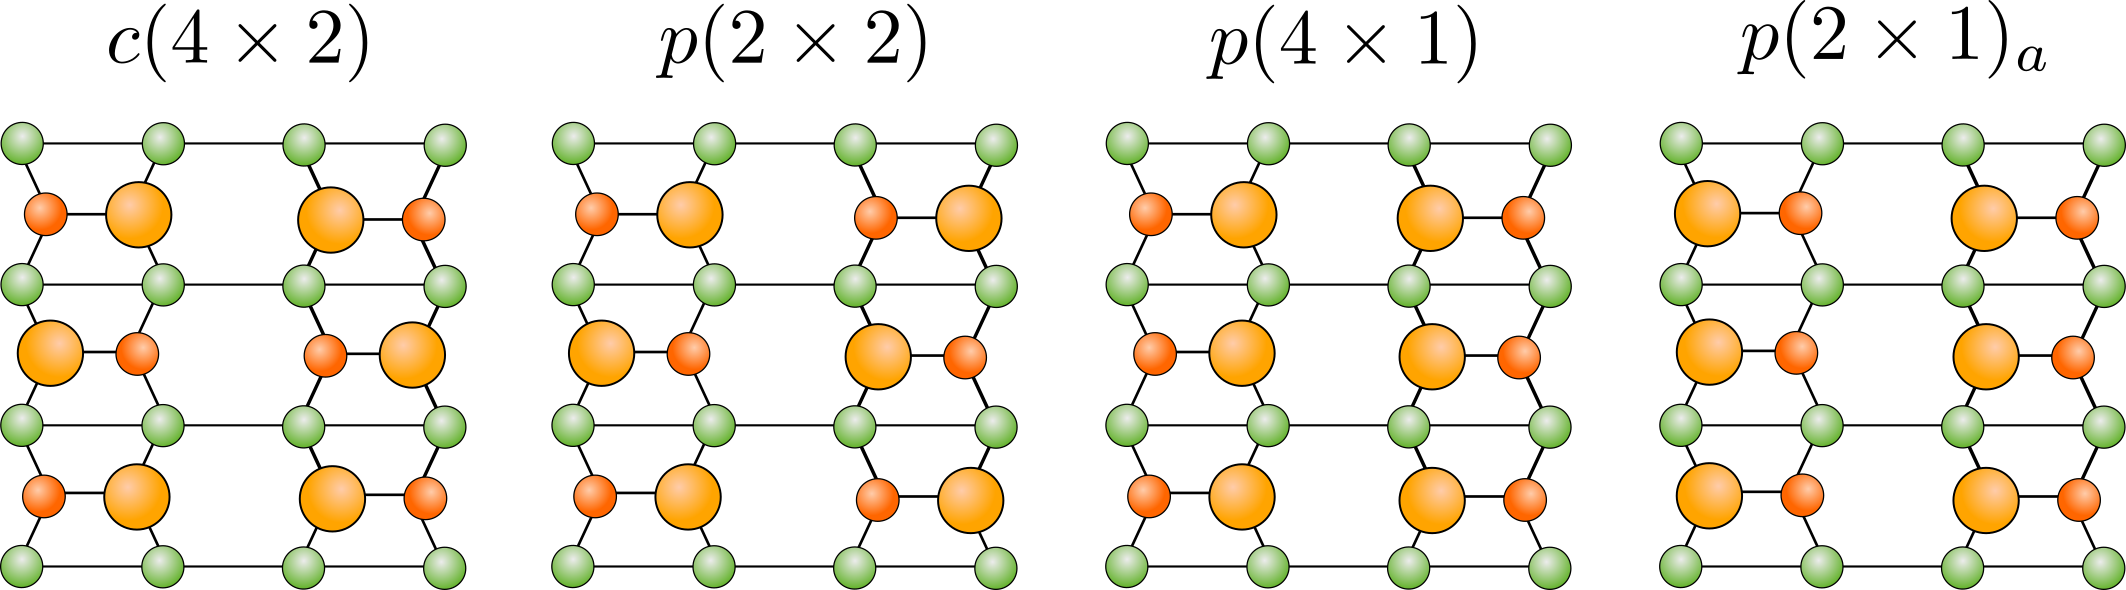
\includegraphics[width=\textwidth]{graphics/surface-configurations-2.png}
		\caption{Slabs of the relevant Si(001) reconstructions are shown from a top down perspective. The upwards buckled dimers are colored in light orange and the downwards buckled dimers in dark orange. The subscript $a$ at the $p(2 \times 1)$ reconstruction denotes that the dimers are asymmetrically buckled.}
		\label{Figure::surface-configurations}
	\end{figure}	
	%	\begin{align}
		%		&\left(\cos(4\vartheta^{(2)} - \cos(4\vartheta^{(1)}) \right)&J_\parallel&+&\left(1-\cos(4\vartheta^{(1)}) \right)&J_\perp&-&2\left(1-\cos(4\vartheta^{(1)}) \right)&J_\times+& \left(\cos \left(\vartheta^{(2)}p\right) - \cos \left(\vartheta^{(1)}p\right)\right) &h =	E_0 + E^{(2)} \\
		%		&\left(1-\cos(4\vartheta^{(1)}) \right)&J_\parallel&+&\left(1-\cos(4\vartheta^{(1)}) \right)&J_\perp&+&2\left(1+\cos(4\vartheta^{(1)}) \right)&J_\times+&\left(\cos \left(\vartheta^{(3)}p\right) - \cos \left(\vartheta^{(1)}p\right)\right) &h =	E_0 + E^{(3)} \\
		%		&J_\parallel&+&\cos\left(4\vartheta^{(4)}\right)&J_\perp&+&2\cos(4\vartheta^{(4)})&J_\times+&\cos \left(\vartheta^{(4)}p\right) &h =	E_0 + E^{(4)} \\
		%		&J_\parallel&+&&J_\perp&+&2&J_\times+&\cos \left(\frac{\pi}{2}p\right) &h =	E_0 + E^{(5)}
		%	\end{align}
	%	Approximating that $\varphi^{(i)} =	19^\circ$ so $\vartheta^{(i)} = \vartheta =	81^\circ =	1.24 $ the prior equation system simplifies to	
%	\begin{equation}
%			\begin{split}
%			0\cdot& J_\parallel& &+ \left(1-\cos(4\vartheta)\right)& &J_\perp& &+&2\left(\cos(4\vartheta) - 1\right)&J_\times&+&0\cdot h&=~& E_{p(2\times2)}, \\
%			\left(1-\cos(4\vartheta) \right)& J_\parallel& &+ \qquad \qquad 0\cdot& & J_\perp& &+&2\left(\cos(4\vartheta)-1 \right)&J_\times&+&0\cdot h&=~& E_{p(4\times1)}, \\
%			\left(1-\cos(4\vartheta) \right)&J_\parallel&
%			&+\left(1 - \cos\left(4\vartheta \right)\right)& &J_\perp& &
%			+&\qquad \qquad 0&J_\times&
%			+&0\cdot h&
%			=~&E_{p(2\times1)}.
%		\end{split}
%	\end{equation}
	\begin{equation}
	\begin{split}
		0\cdot J_\parallel&+ \left(1-\cos(4\vartheta)\right)J_\perp&+&2\left(\cos(4\vartheta) - 1\right)J_\times&+&0\cdot h= E_{p(2\times2)}, \\
		\left(1-\cos(4\vartheta) \right) J_\parallel&+ \qquad \qquad ~~ 0\cdot  J_\perp&+&2\left(\cos(4\vartheta)-1 \right)J_\times&+&0\cdot h= E_{p(4\times1)}, \\
		\left(1-\cos(4\vartheta) \right)J_\parallel
		&+\left(1 - \cos\left(4\vartheta \right)\right) J_\perp&+& \qquad \qquad \quad ~ 0\cdot J_\times&
		+&0\cdot h
		=E_{p(2\times1)}.
	\end{split}
\end{equation}
	In the $\vartheta =	\text{const.}$ approximation, these equations are independent of $h$. Additional configurations will be used shortly to approximate $h$.
	Solving with the PBEsol values of \cite{brand2023critical} yields
	\begin{equation}
		J_\parallel =	115.6 \text{ meV} , \qquad \qquad J_\perp =	-17.3 \text{ meV} \qquad \text{and} \qquad J_\times =	-9.5 \text{ meV} \\		
	\end{equation}
	Because of the strong anisotropy, it is possible to calculate an effective $J_\perp$ across the dimer rows from $J_\perp$ and $J_\times$. The new $J_\perp$ becomes 
	\begin{equation}
		J_\perp - 2 J_\times \qquad \rightarrow  \qquad J_\perp =	1.7 \text{ meV} ~.
	\end{equation}
	The XY critical temperature obtained from these coupling constants 
	\begin{equation}
		T_c^{\text{XY}} =	18.87 \text{ meV}
	\end{equation}
	is in proximity of the experimental critical temperature \eqref{Eq::Exp-Tc}. However, the ratio $J_\parallel /	J_\perp = 68$ is much larger.\\
	
	Dabrowski and Scheffler \cite{dabrowski1992self} describe the movement of the dimer to be in a double well potential with a barrier height of $E_B =	100 \text{ meV}$. The same argumentation can be applied to \cite{inoue1994order}, leading to $E_B =	170 \text{ meV}$. Recent calculations from Kratzer \cite{kratzer2024flip} model a dimer row consisting of five dimers. The dimers are buckled antisymmetrically  except for a domain boundary. The simulations describe the advance of the defect by flipping the dimer at the boundary. During the process, the dimer takes on a horizontal position. The energy difference per dimer between the domain boundary state $E_{\text{DB}}$ and the horizontal state $E_\text{H}$ is calculated to be 
	\begin{equation} \label{Eq::Flip-Energy}
		\begin{split}
			E_\text{H} - E_{\text{DB}} = J_\parallel \left(2 \cos ( 2 (\vartheta - \pi / 2)) -1 - \cos(4 \vartheta)\right) &+ 2 J_\times \left(\cos(\pi + 2 \vartheta) - 1 - \cos(4 \vartheta) \right) \\
			&+ h \left(\cos(\pi p /	2) - \cos(\vartheta p)\right),
		\end{split}
	\end{equation}
	with $E_\text{H} - E_\text{DB} =	74 \text{meV}$. Using Eq. \eqref{Eq::Flip-Energy} and Eq. \eqref{Eq::Equilibrium-Position} as well as the above values for the coupling constants  to fit $h$ and $p$ yields
	\begin{align}
		&h =	1282 \text{ meV} \qquad \text{and} \qquad p =	2.28~.
	\end{align}
	Hence, the symmetry breaking field in the experimental system is much stronger than the dimer interactions 
	\begin{equation} \label{Eq::h-J-ratio}
		h \approx 10 J_\parallel~.
	\end{equation}
	Note that the preceding considerations serve for a qualitative assessment of the considered model and have no claim to be quantitatively correct.
	\section{Static Scaling}
	In the following the results of the laid out simulation will be presented. We will start with the examination of the static properties of the adapted anisotropic XY model. \\
	
	The coupling constants of Eq.~\eqref{Eq::Exp-coupling-ising} are used as a starting point.
	 The external field is initially chosen small compared to $J_\parallel$ to ensure approximate validity of Eq.~\eqref{Eq::Crit-Temp-XY}. The dimensionless parameters given by Eq.~\eqref{Eq::dimensionless-coupling} are set to
	\begin{equation} \label{Eq::standard-parameters}
		j_\perp =	-3500~, \qquad \qquad j_\parallel =	-110000 \qquad \text{and} \qquad \rho =	10000.
	\end{equation}
	The dampening is fixed to $\eta =	1$ and $p=2.5$ for now. \\
	
	The correlation length extraction, see \autoref{Section::Corr-Length-Calculation}, works best if $\xi_\delta \ll L_\delta$. Since the Si(001) surface exhibits a large correlation length anisotropy ${(\xi^+_\parallel /	a_\parallel)} /	{(\xi^+_\perp /	a_\perp)} \approx 10 $ \cite{brand2023critical}, it is useful to ensure that the system dimensions share a similar ratio. This way the computational cost can be optimized to analyze as large as possible correlation lengths. The following systems have a ratio of ${L_\parallel} /	{L_\perp} =	8$ if not stated otherwise. The used step size of
	\begin{equation}
		\text{d}\sigma = 10^{-5}
	\end{equation}
	is validated in \autoref{Section::Benchmarks}.
	
	
	
	\subsection{Measurement of Observables} \label{Section::observable-measurement}
	All observables that we are trying to measure are subject to fluctuations due to the thermal interaction. Usually of interest are the \textbf{ensemble averages} of systems in \textbf{thermal equilibrium}. \\
	
	The ensemble average is calculated by computing the desired observable for many different realizations of the same system. The \textbf{ergodic hypothesis} assumes that the average of many realizations and the average over one system for long times are the same. We assume that our system is ergodic. Since GPU accelerated programming is employed, we want to fully utilize the GPU. Systems should be simulated that are large enough to max out the graphical processing unit. Depending on the GPU, good utilization is usually reached for systems with about $N=  5 \cdot 10^5 - 1 \cdot 10^6$ lattice sites. For many use cases, like calculating the Binder cumulant $U_L$, such large systems are not needed. Therefore, always $n \approx	N /	(L_\parallel L_\perp)$ independent subsystems are simulated. These systems are used in combination with the ergodic hypotheses to get the best ensemble averages available. For a simulation of $n$ subsystems for a time of $t$ the ensemble average of a quantity $f_i$ of system $i$ is calculated via
	\begin{equation} \label{Eq::ensemble-average-calculation}
		\langle f \rangle = \frac{1}{n \cdot t} \sum_i^n \int_0^{t} \text{d}s f_i(s)~.
	\end{equation}
	 When making use of the ergodic hypotheses to calculate equilibrium quantities, it is important to make sure that the system is actually equilibrated. Usually a lower time bound $t_0$ is introduced to account for the relaxation time. Again, the relaxation time is not known and therefore $T_0$ set to a fraction of $T$ to eliminate strong fluctuations in the equilibration phase of the simulation. To eventually judge the relaxation of the system, the error of Eq.~\eqref{Eq::ensemble-average-calculation} is considered. The approach is that the equilibration introduces a large statistical deviation on the average $\langle f \rangle$. So by calculating the error $\Delta \langle f \rangle $ we can extract some information about the state of equilibration of the system. The $f(s)$ are correlated for different time points. The strength of the correlation depends on how quickly or slowly the system relaxes. To get reasonable estimates on the error of $\langle f \rangle$ we have to judge how many effectively independent measurements of $f$ are taken by the $\text{d}s$ integration in Eq. \eqref{Eq::ensemble-average-calculation}. The error calculation for a time series $f_i(s)$ is done in  \autoref{Section::Error-Calc}. Analyzing $f_i(s)$ as time series helps to avoid terminating the simulation too early for slowly relaxing systems. Additionally, it gives an estimate for how many measurements should be recorded in order not to overflow with data. \\
	 
	 On the run, $f_i(s)$ is calculated and saved for discrete time steps $\text{d}s$. The measurement time step $\text{d}s$ is usually much larger then the integration step size $\text{d}\sigma$
	 \begin{equation}
	 	\text{d}s \gtrsim 100 \cdot \text{d}\sigma,
	 \end{equation}
	 to limit the amount of data generation. The exact value depends on the integrated autocorrelation time $\tau_C$ \eqref{Eq::Autocorrelation-Time} and is adapted on the run
	 \begin{equation}
	 	 \text{d}s \approx \frac{1}{10} \tau_C~.
	 \end{equation}
	\subsection{The Critical Temperature} \label{Section::crit-temp}
		As mentioned, the critical temperature of the used model is not analytically calculable. To numerically determine the critical temperature the in \autoref{Sec::Binder-Cumulant} introduced Binder cumulant is employed. As a reminder, the Binder cumulants for two different system sizes $L_1$ and $L_2$ intersect at the critical point $\varepsilon = 0$
		\begin{equation}
			U_{L_1} (0) =	U_{L_2} (0) =	U^*~.
		\end{equation}
		Computing $U_{L}(\varepsilon)$ and determining the intersection directly yields the critical temperature. The binder cumulant is calculated from the ensemble averages of the second and fourth moment of the lattice average Eq. \eqref{Eq::lattice-average}. Hence, $M_L(s)$ defined as in Eq. \eqref{Eq::Si-Order-Param} is recorded during the run. The termination condition for the simulation is the error on $U_L$ which is given by standard error propagation and the errors on $\left \langle M_L^2 \right \rangle$ and $\left \langle M_L^4 \right \rangle$ as in \autoref{Section::Error-Calc}. \\
		\begin{figure}[tb]
			\begin{subfigure}{0.475\textwidth}
				\centering
				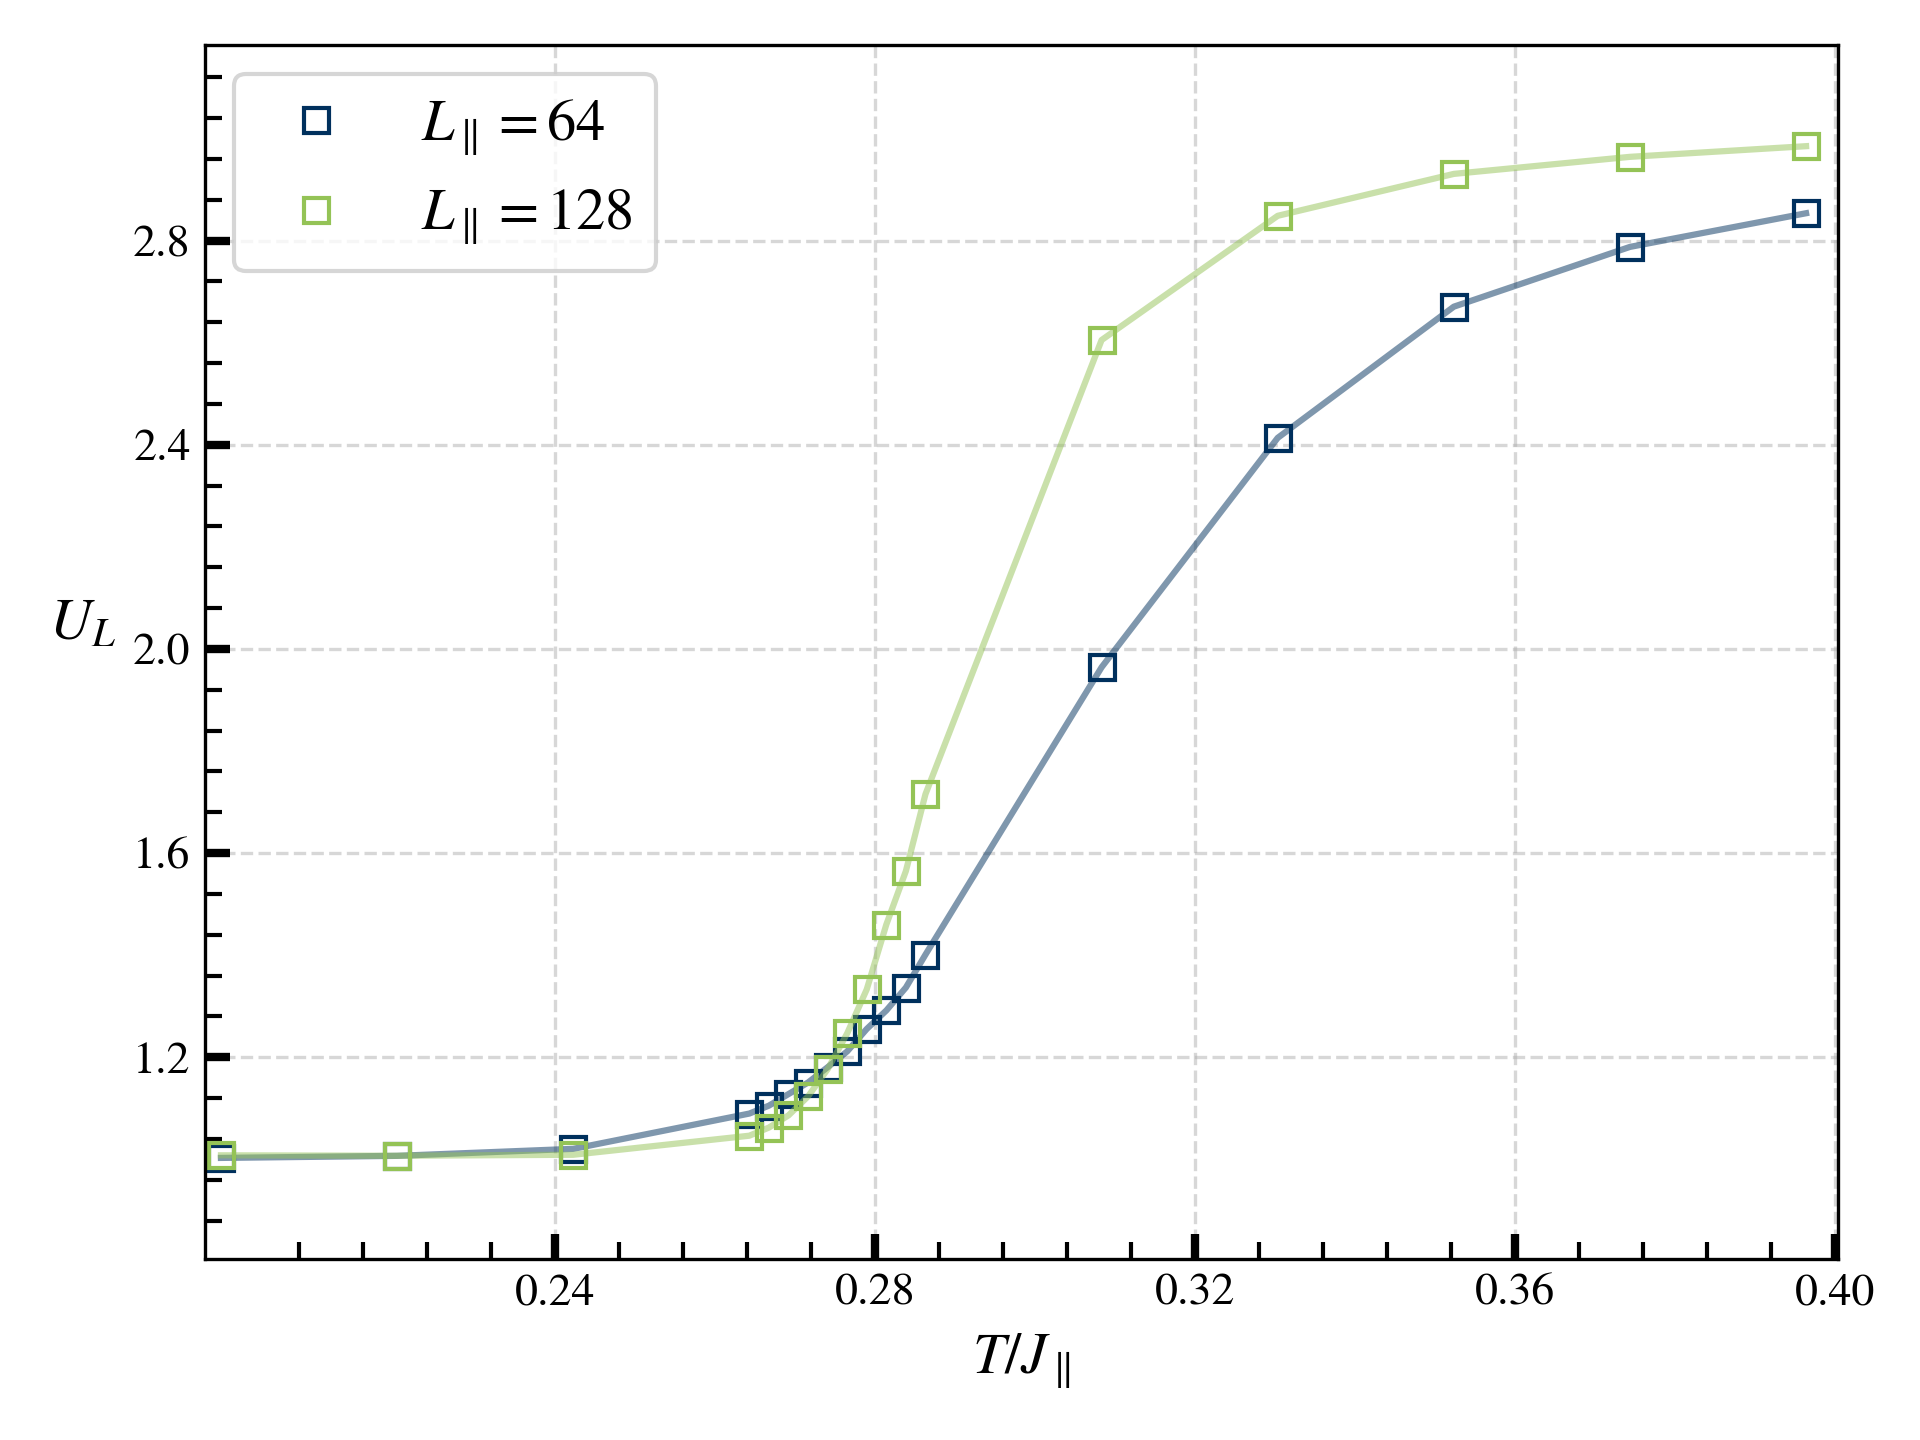
\includegraphics[width=0.95\linewidth]{graphics/cum_time_avg-Tc.png}
			\end{subfigure}
			\begin{subfigure}{0.475\textwidth}
				\centering
				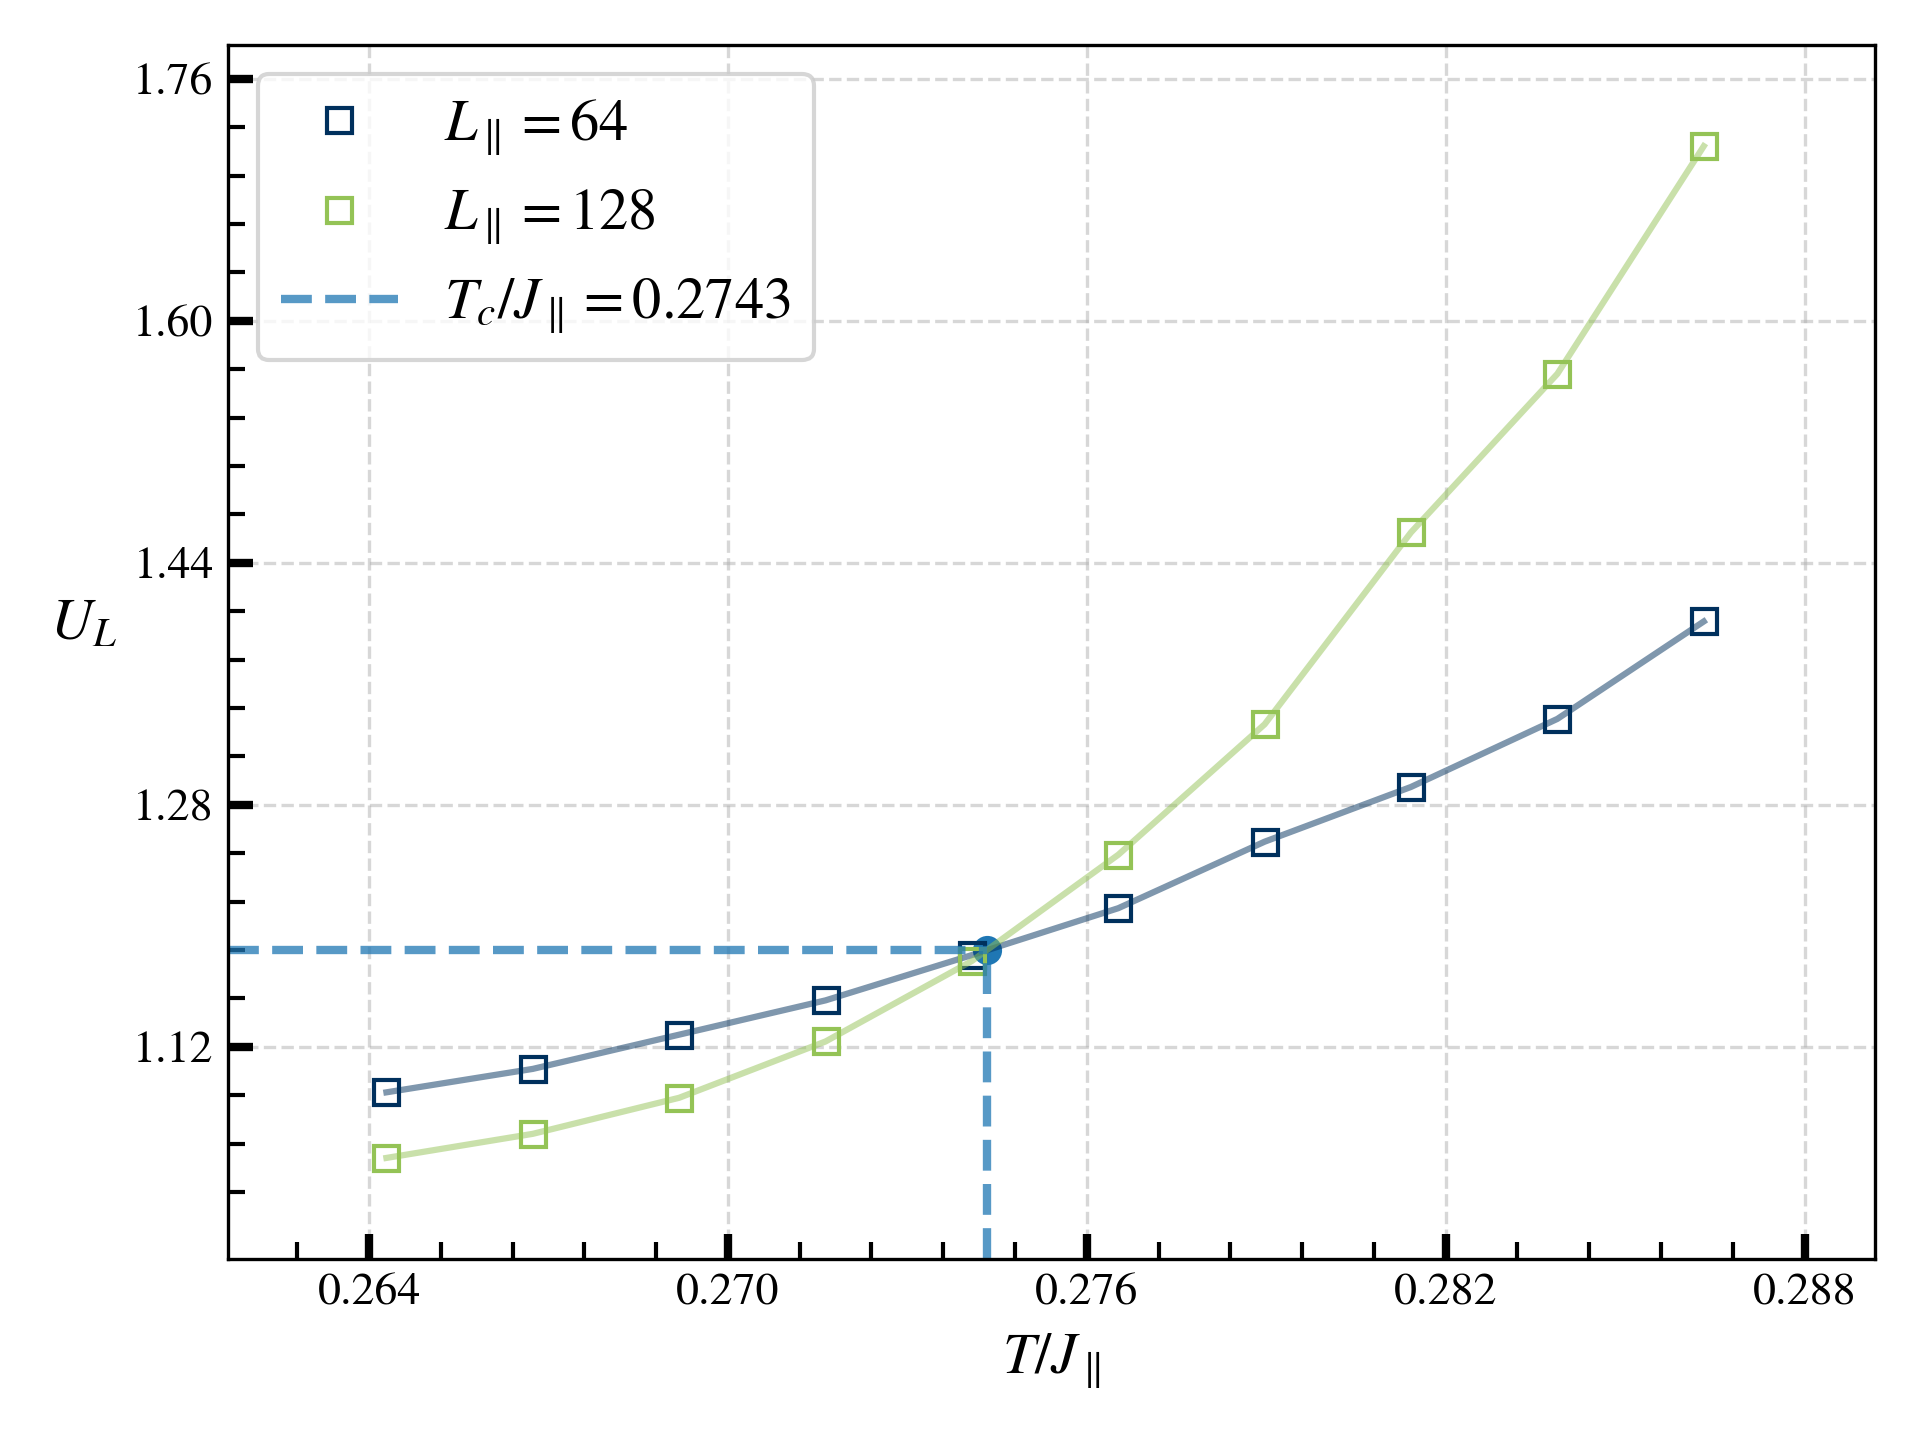
\includegraphics[width=0.95\linewidth]{graphics/cum_time_avg-Tc-zoom.png}
			\end{subfigure}
			\caption{The Binder cumulant $U_L$ is shown in dependence of the temperature for the system sizes $L_1 =	64$ and $L_2 =	2 L_1 =	128$. The measured data points are squares connected by linear interpolations to guide the eye. The system parameters are defined in \eqref{Eq::standard-parameters}. \textbf{(a)} A course measurement for ten temperatures with $T_{\text{min}} =	T_c^{\text{XY}}$ and $T_{\text{max}} =	2T_c^{\text{XY}}$ yields an already fine estimate for $T_c$. \textbf{(b)} In the interval of the intersection, ten more measurements are performed to get a precise estimate of the critical temperature. The intersection at $T_c /	J_\parallel =	0.2743  \pm 0.0012$ is marked with a dashed line.}
			\label{Fig::Binder-Cum-Intersection}
		\end{figure}
	
		Eq.~\eqref{Eq::Crit-Temp-XY} is used to initially guess the critical temperature. It is expected that the parameter $h$ increases $T_c$ in a manner that has been shown by Jose et. al \cite{jose1977renormalization}. The critical strength of the symmetry breaking field $h_c$ according to them behaves as
		\begin{equation} \label{Eq::h_c-T-dependence}
			h_c \propto e^{-AT^2 e^{B/T}}~,
		\end{equation}
		with constants $A$ and $B$ . This equation is valid for small $h_c$. \\
		
		 Results for the measurement of $L_1 =	64$ and $L_2 =	128$ with periodic boundary conditions are shown in \autoref{Fig::Binder-Cum-Intersection}. Note that the value of $U^*$ depends on the intersection and the shape of the system, but not its location.  The systems are started from a totally ordered state. The determined effective critical temperature is
		\begin{equation} \label{Eq::crit-temp-exp-values}
			T_c /	J_\parallel  = 0.2743 \pm 0.0012	
		\end{equation}
		at
		\begin{equation} \label{Eq::crit-h-exp-values}
			\beta_c h = 0.3314 \pm 0.0030.
		\end{equation}
		Comparing with Eq.~\eqref{Eq::Tc-XY-31} confirms that the critical temperature is significantly influenced by the the symmetry breaking field. The error on the critical temperature is conservatively estimated to be half of the interval step size $\Delta T_c =	\tfrac{1}{2} \text{d}T$. \\
		
		 Computations with the actual experimental parameters from \autoref{Section::quantitative} have proven to be difficult to simulate. The same is the case with the $J_\parallel / h$-ratio of Eq. \eqref{Eq::h-J-ratio}. The height of the potential barrier slows down the dynamics \textcolor{red}{(citation)} of the system significantly. For the Langevin dynamics simulation at hand, this leads to an enormous increase in computation effort.  Their simulation is at the moment not feasible. However, scale invariant and universal properties will still be valid, so we will proceed with $j_\delta \approx 1$ and $h \simeq j_\delta$. The following dimensionless couplings
		 \begin{equation} \label{Eq::good-dimensionless-parameters}
		 	j_\parallel =	3.110, \qquad j_\perp = 0.100 \qquad \text{and} \qquad \rho = 0.283 ~,
		 \end{equation}
	 	will be used according to Eq. \eqref{Eq::crit-temp-exp-values} and \eqref{Eq::crit-h-exp-values}. It will be shown soon that they, as expected, reproduce the critical point just measured. At the moment it is not sorted out why the coupling constants around $j_\delta \approx 1$ are better behaved since physically, they should just describe a completely analogous system that is simply weaker coupled. A weaker coupling can be integrated by a larger step size, but the dynamics also slow down. Computation time wise, the two cases should be equivalent. However, this shall not bother us any longer since it is expected that the scales ar invariant to all extents.
	\subsubsection{Finite-size effects on $\boldsymbol{T_c}$}
	Due to corrections to FSS the position of the intersection can scatter for small $(L_1, L_2)$ pairs. In \autoref{Fig::Tc-L-dependence}, the computed $T_c(L_1)$ is shown in dependence of the system size $L_1$. Again, the data points show the intersection of two curves $U_{L_1}(T)$ and $U_{L_2}(T)$ with $L_2 =	2 L_1$. The simulations were performed using the parameters of Eq. \eqref{Eq::good-dimensionless-parameters}. The difference in $T_c(L_1)$ is negligible between $T_c(40)$ and $T_c(64)$ so we conclude that the corrections to FSS for the critical temperature determination vanish on these length scales.  \\
	
	Note that measurements like shown in \autoref{Fig::Tc-L-dependence} are computationally expensive. The cumulant $U_L(\varepsilon)$ has to be measured for about ten different system sizes at about ten different temperatures to get a reasonable $T_c$ estimation. This while being subject to thermal fluctuations and critical slowing down. Depending on $L$ and the desired precision, the runtime for a single data point approaches or even exceeds one hour.  Roughly estimated, the computation time for \autoref{Fig::Tc-L-dependence}. approaches 100 hours. Efficient algorithms are therefore vital (see \autoref{Section::efficient-crit-temp}).
	\begin{figure}[tb]
		\centering
		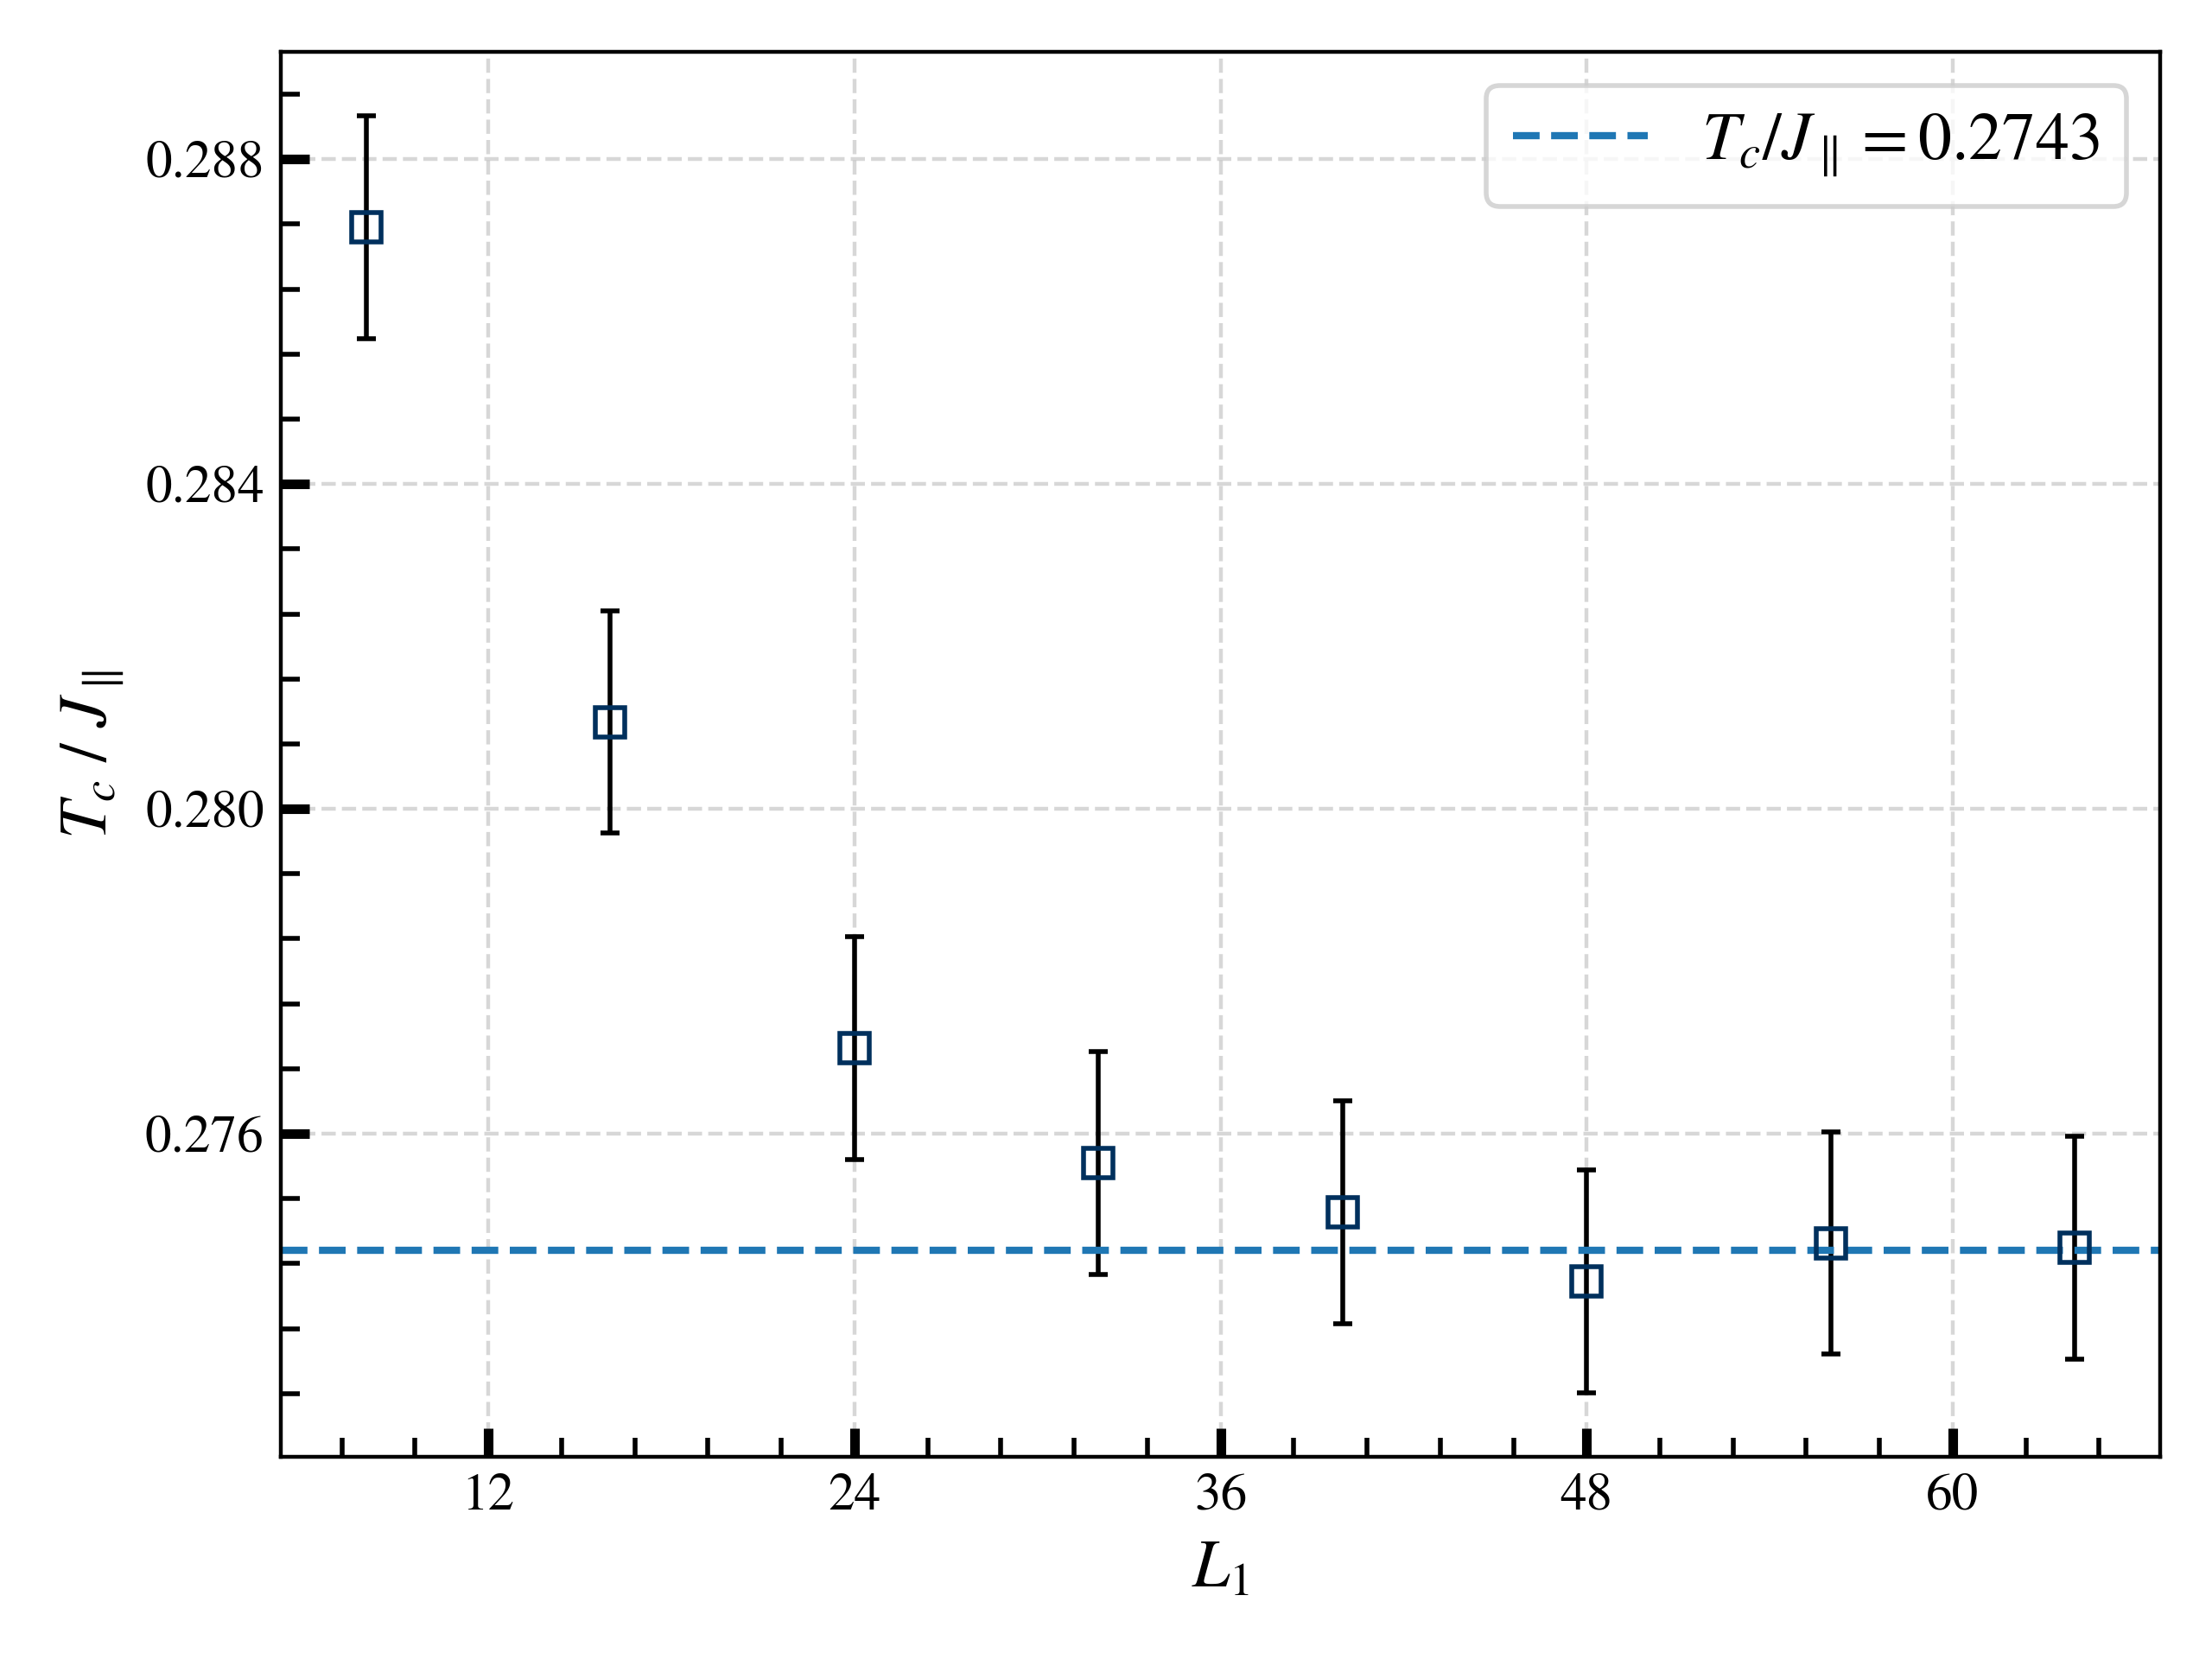
\includegraphics[width=0.8\linewidth]{graphics/Tc_L-5.png}
		\caption{The dependence of the critical temperature $T_c(L_1)$ on the system size is shown. The Binder cumulant intersection is calculated between $L_1$ and $L_{2} =	2 L_{1}$. The uncertainties are estimated to be half of the temperature step size $\text{d}T /	J_\parallel = 0.0027$ that has been used to determine the intersection. Between the largest recorded system sizes the difference of $\Delta T_c /	J_\parallel = 10^{-4}$ is negligible and much smaller than the uncertainties. The simulations were performed using the parameters of Eq. \eqref{Eq::good-dimensionless-parameters}. The result $T_c(64) / J_\parallel =	0.2743$ of \autoref{Fig::Binder-Cum-Intersection} is shown as a dashed line. The effective critical temperature is indeed invariant between the two parameter sets.}
		\label{Fig::Tc-L-dependence}
	\end{figure}
	\subsection{The Critical Exponent $\boldsymbol{\nu}$} \label{Section::static-scaling}
	Since the phase transition of the Si(001) surface shows good agreement with the Ising universality class \cite{brand2023critical}, our simulation should reproduce this. The XY model with a $p$-fold symmetry breaking external field belongs to the Ising universality class for $p=2$ \cite{jose1977renormalization}. The question remains if this is still true for our adaptation with rational $p \approx 2.5$ and a reduced phase space. \\
	
	Therefore, the finite size techniques of \autoref{Section::FSS} and the Binder cumulant are employed to extract the critical exponent. The measurements of \autoref{Fig::Tc-L-dependence} can be reused to calculate the derivative $\tfrac{\partial U_L}{\partial \varepsilon}$ in dependence of the system size.
	In \autoref{Fig::Binder-Cum-Result} the results for selected $L \in \left[8, 128\right]$ are shown for temperatures very close to $T_c$. Small temperature differences between the data points require small errors to resolve the differences in $U_L$. The derivative $\tfrac{\partial U_L}{\partial \varepsilon}$ is calculated through a central difference. Afterwards, Eq.~\eqref{Eq::FSS-dU_dT} is fitted to $\tfrac{\partial U_L}{\partial \varepsilon} (L)$. The result $\nu =	1.01$ is in excellent agreement with the Ising exponent $\nu =	1$.
	\begin{figure}[tbh]
		\begin{subfigure}{0.475\textwidth}
			\centering
			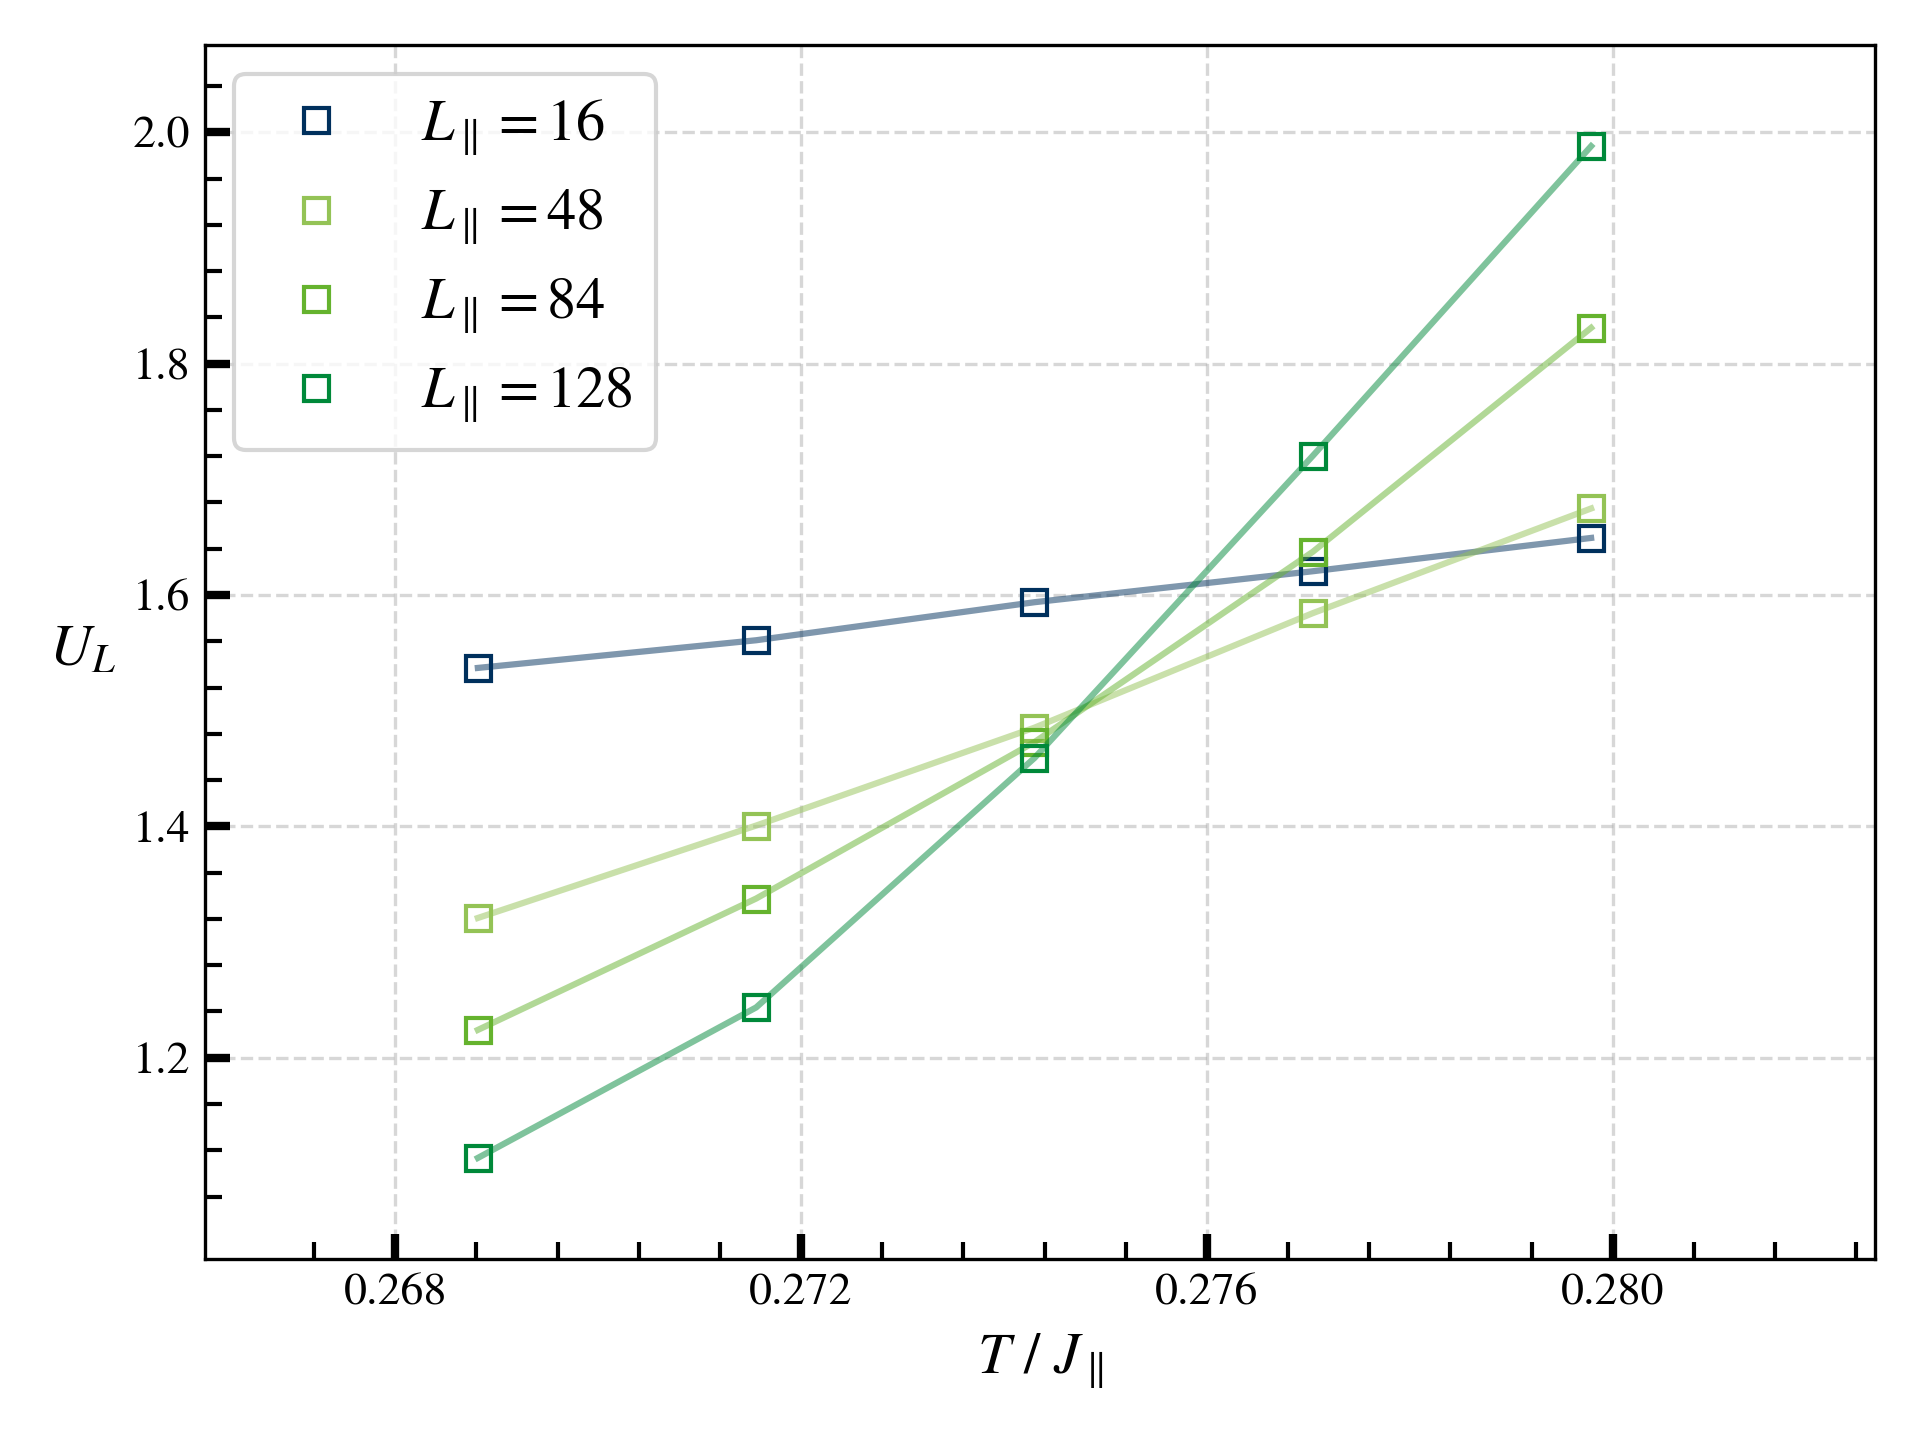
\includegraphics[width=0.95\linewidth]{graphics/slope-at-critical-point-3.png}
		\end{subfigure}
		\begin{subfigure}{0.475\textwidth}
			\centering
			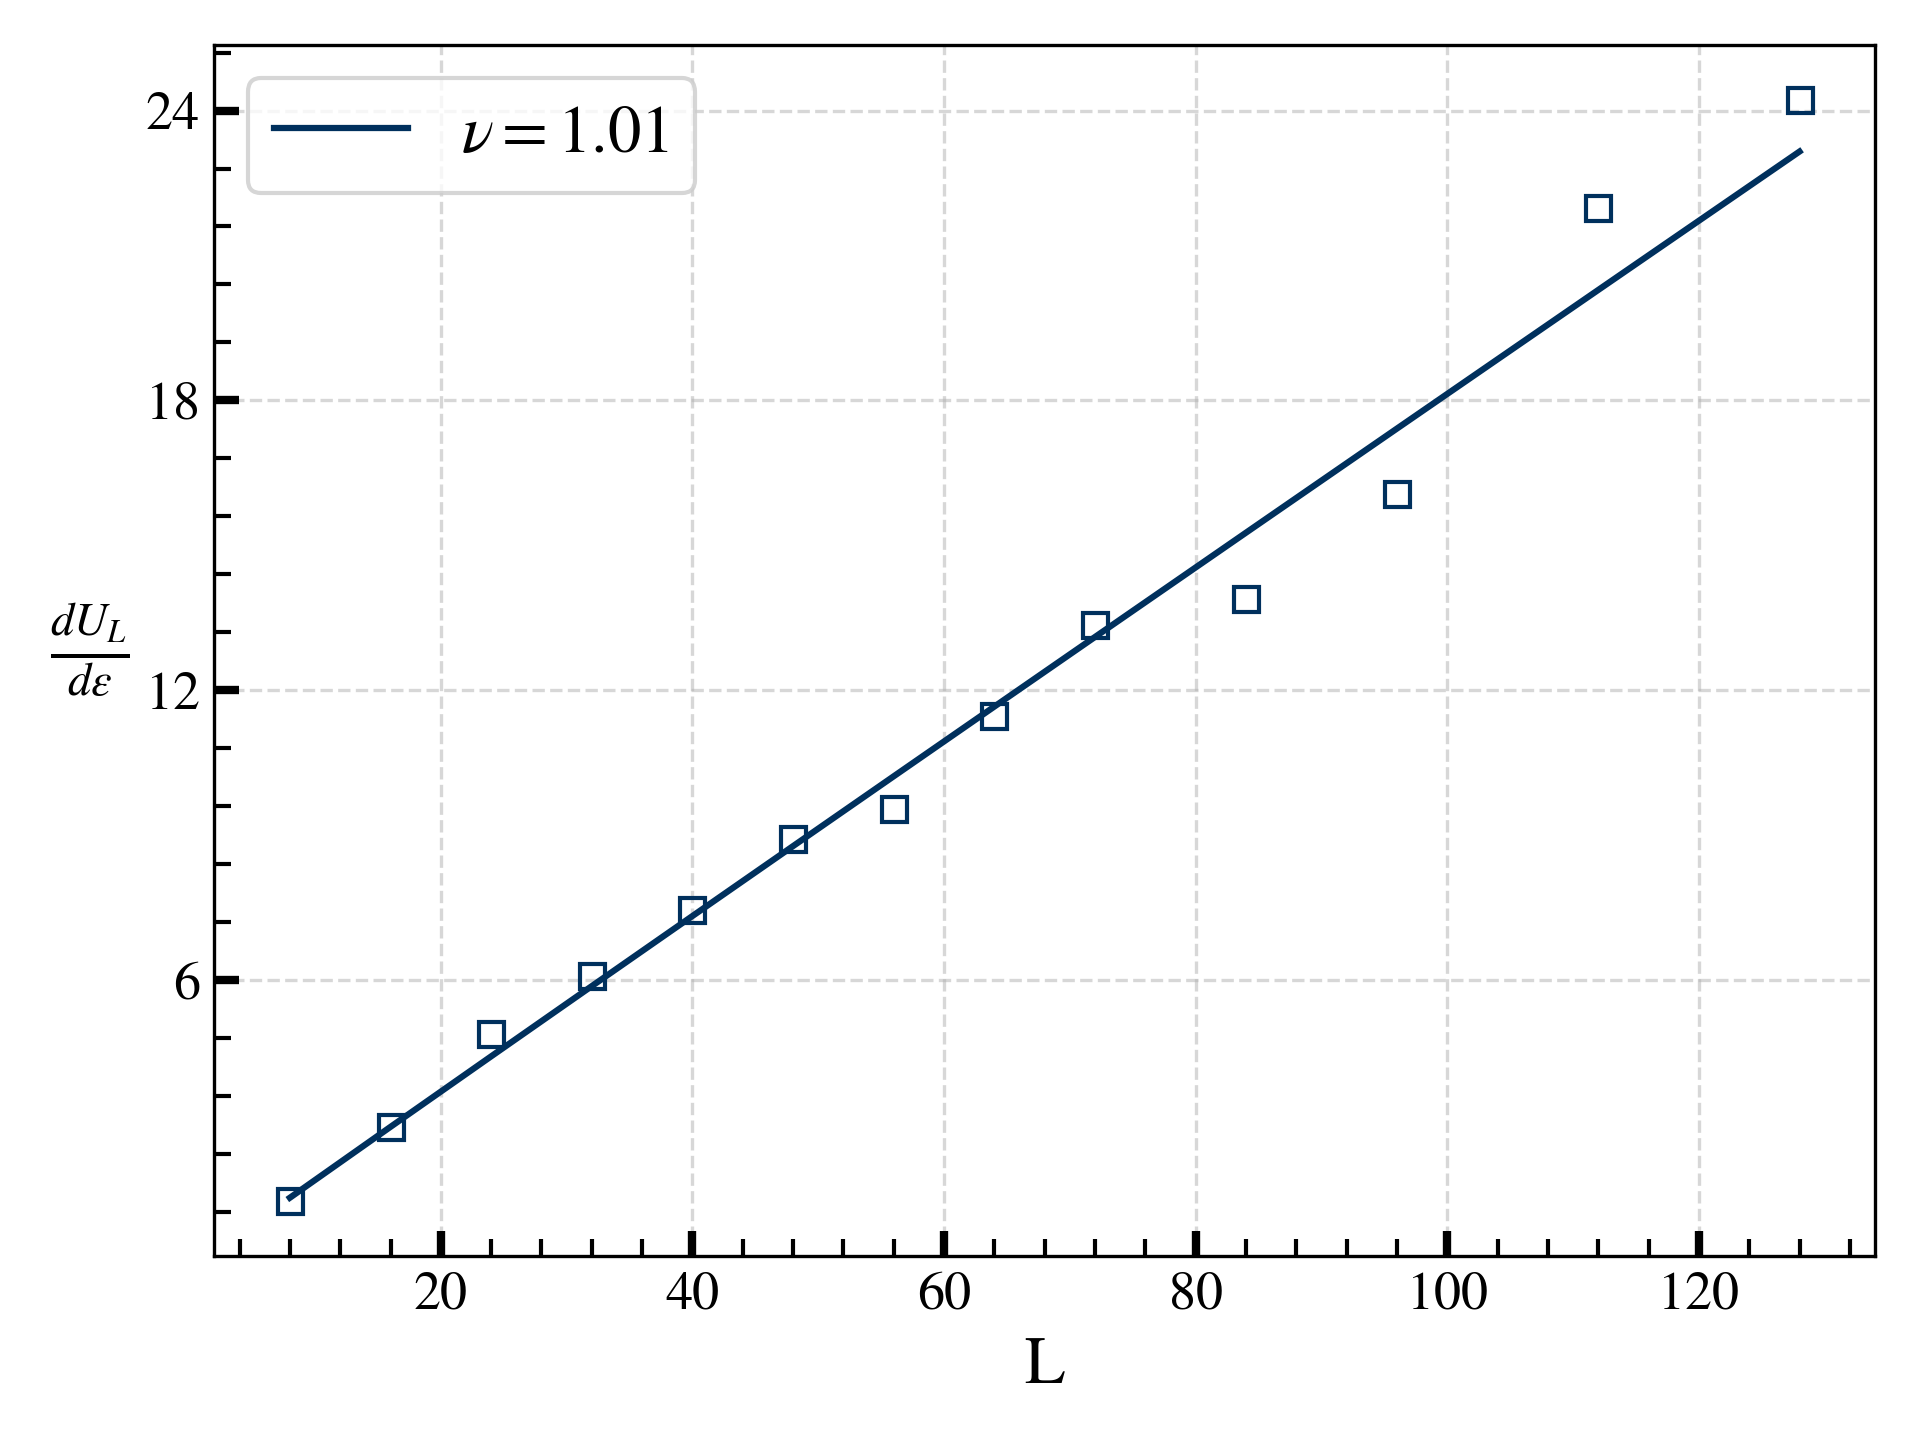
\includegraphics[width=0.95\linewidth]{graphics/nu-2.png}
		\end{subfigure}
		\caption{\textbf{(a)} The results of ${U}_L(\varepsilon)$ for selected sizes $L \in \left[8, 128\right]$ is measured close to the critical point. Ignoring finite size corrections, all cumulants intersect approximately at the same point $(\beta_c J_\parallel)^{-1} = 0.2743$. \textbf{(b)} The derivatives $\frac{\partial U_L}{\partial \varepsilon} \propto L^\nu$ are shown in dependence of the system size. The derivatives are calculated using a standard central difference method with the data points of (a). The fitting yields $\nu = 1.01$ which is in good accordance with the Ising model.}
		\label{Fig::Binder-Cum-Result}
	\end{figure}
	The matching of the static critical exponent verifies the assumption that the modified XY model still belongs to its expected universality class. \\

	
	\subsection{Phase Diagram} \label{Section::Phase-Diagram}
	The result of $\nu = 1$ is strong evidence that also Eq.~\eqref{Eq::h_c-T-dependence} is valid. In order to confirm this assumption, a phase diagram in the $h-T-$plane will be recorded. This is a computationally intensive task as it requires the measurement of many critical temperatures. An efficient and mostly autonomous algorithm for the $T_c$ estimation is therefore important.
	
	\subsubsection{Efficient $\boldsymbol{T_c}$ determination} \label{Section::efficient-crit-temp}
	For the computation of $T_c$ and $\nu$, only the $U_L$ values in close proximity of $T_c$ are relevant. Of course, $T_c$ is not known beforehand but it is nonetheless desired to spend as little time as possible calculating $U_L$ far away from the phase transition. The relation in Eq. \eqref{Eq::Crit-Temp-XY} is very useful to for an initial $T_c$ guess. Eq. \eqref{Eq::h_c-T-dependence} states that the critical temperature of the symmetry broken XY model is larger than the on of isotropic XY model, so $T_{\text{min}} = T_c^{\text{XY}}$ can be chosen. Experience shows that the critical temperature rarely exceeds $T_{\text{max}} = 2 T_c^{\text{XY}}$. So the first two temperatures that will be recorded will always be $T_c^{\text{XY}}$ and $2T_c^{\text{XY}}$. The difference
	\begin{equation}
		\Delta U (L_1, L_2, \varepsilon) =	|U_{L_1}(\varepsilon) - U_{L_2}(\varepsilon)|,
	\end{equation}
	depends on the actual system sizes. It is desirable to work with large $\Delta U$ to resolve the intersection even when subject to uncertainties. To maximize $\Delta U(L_1, L_2, \varepsilon)$, the difference in system size should be as large as possible while keeping the finite-size effects and computation time to a minimum. The maximization of $\Delta U (L_1, L_2, \varepsilon)$ helps to avoid artificial intersections where $U_{L_1}(\varepsilon) \approx U_{L_2}(\varepsilon)$ that occur through thermal fluctuations. \\
	
	After the initial four measurements, which typically show that $T_c^{\text{XY}}  < T_c < 2 T_c^{\text{XY}}$, four new simulations will be started. The best guess is to select temperatures equally spaced between the just determined boundaries of $T_c$. The two added temperatures divide the initial interval in three subintervals, one of which will contain the critical temperature. The according subinterval is selected as the new bounds and the procedure repeats. As soon as the determined bounds fall below the specified precision, the algorithm is terminated. \textcolor{red}{(Als Pseudocode aufschreiben? Als Enumeration mit steps oder einfach genug um so im Fließtext stehen zu lassen?)} \\
	
	The equilibration time of systems is strongly depending on the initial condition. For example, it takes a long time for a totally unordered high temperature system to reach relax if it is coupled to a low temperature reservoir. Hence, it is useful to initialize systems in states that are already close to their equilibrium. Of course, there is again no way of knowing the equilibrium distribution beforehand. But already performed simulations can be used as initial conditions for new runs . Hence, excluding the initial measurements at $T_c^{\text{XY}}$ and $2T_c^{\text{XY}}$, the previous simulation with temperature closest to the new $T$ will be used as initial state. \textcolor{red}{Schaubild für Arbeitsweise?}
	\subsubsection{The phase diagram}
	As mentioned in \autoref{Section::crit-temp}, the symmetry breaking field has a strong influence on the dynamics of the system. The dynamics and the relaxation significantly slows down at $ h / J_\parallel \approx 1$. Systems with larger $h$ are not feasible to simulate and are omitted in the phase diagram. \\
	
	The measured phase diagram for the parameters of \eqref{Eq::standard-parameters} and \eqref{Eq::good-dimensionless-parameters} is shown in \autoref{Fig::Phase-Diagram-h}. It roughly follows the behavior predicted by José et. al \cite{jose1977renormalization}. The constants of \eqref{Eq::h_c-T-dependence}, or in other words the shape of the phase boundary, only dependent on the ratio $J_\parallel /	J_\perp$. The $\beta h_c(T)$ curves collapse for different quantitative values of the dimensionless coupling $j_\delta$ if $T$ is divided by $J_\parallel$. The prediction by Eq. \eqref{Eq::h_c-T-dependence} seems to overestimate the slope of $h_c(T)$. However, this could also be an effect of the strong anisotropy of the coupling constants.	
	\begin{figure}[htp]
		\begin{subfigure}{0.9\textwidth}
			\centering
			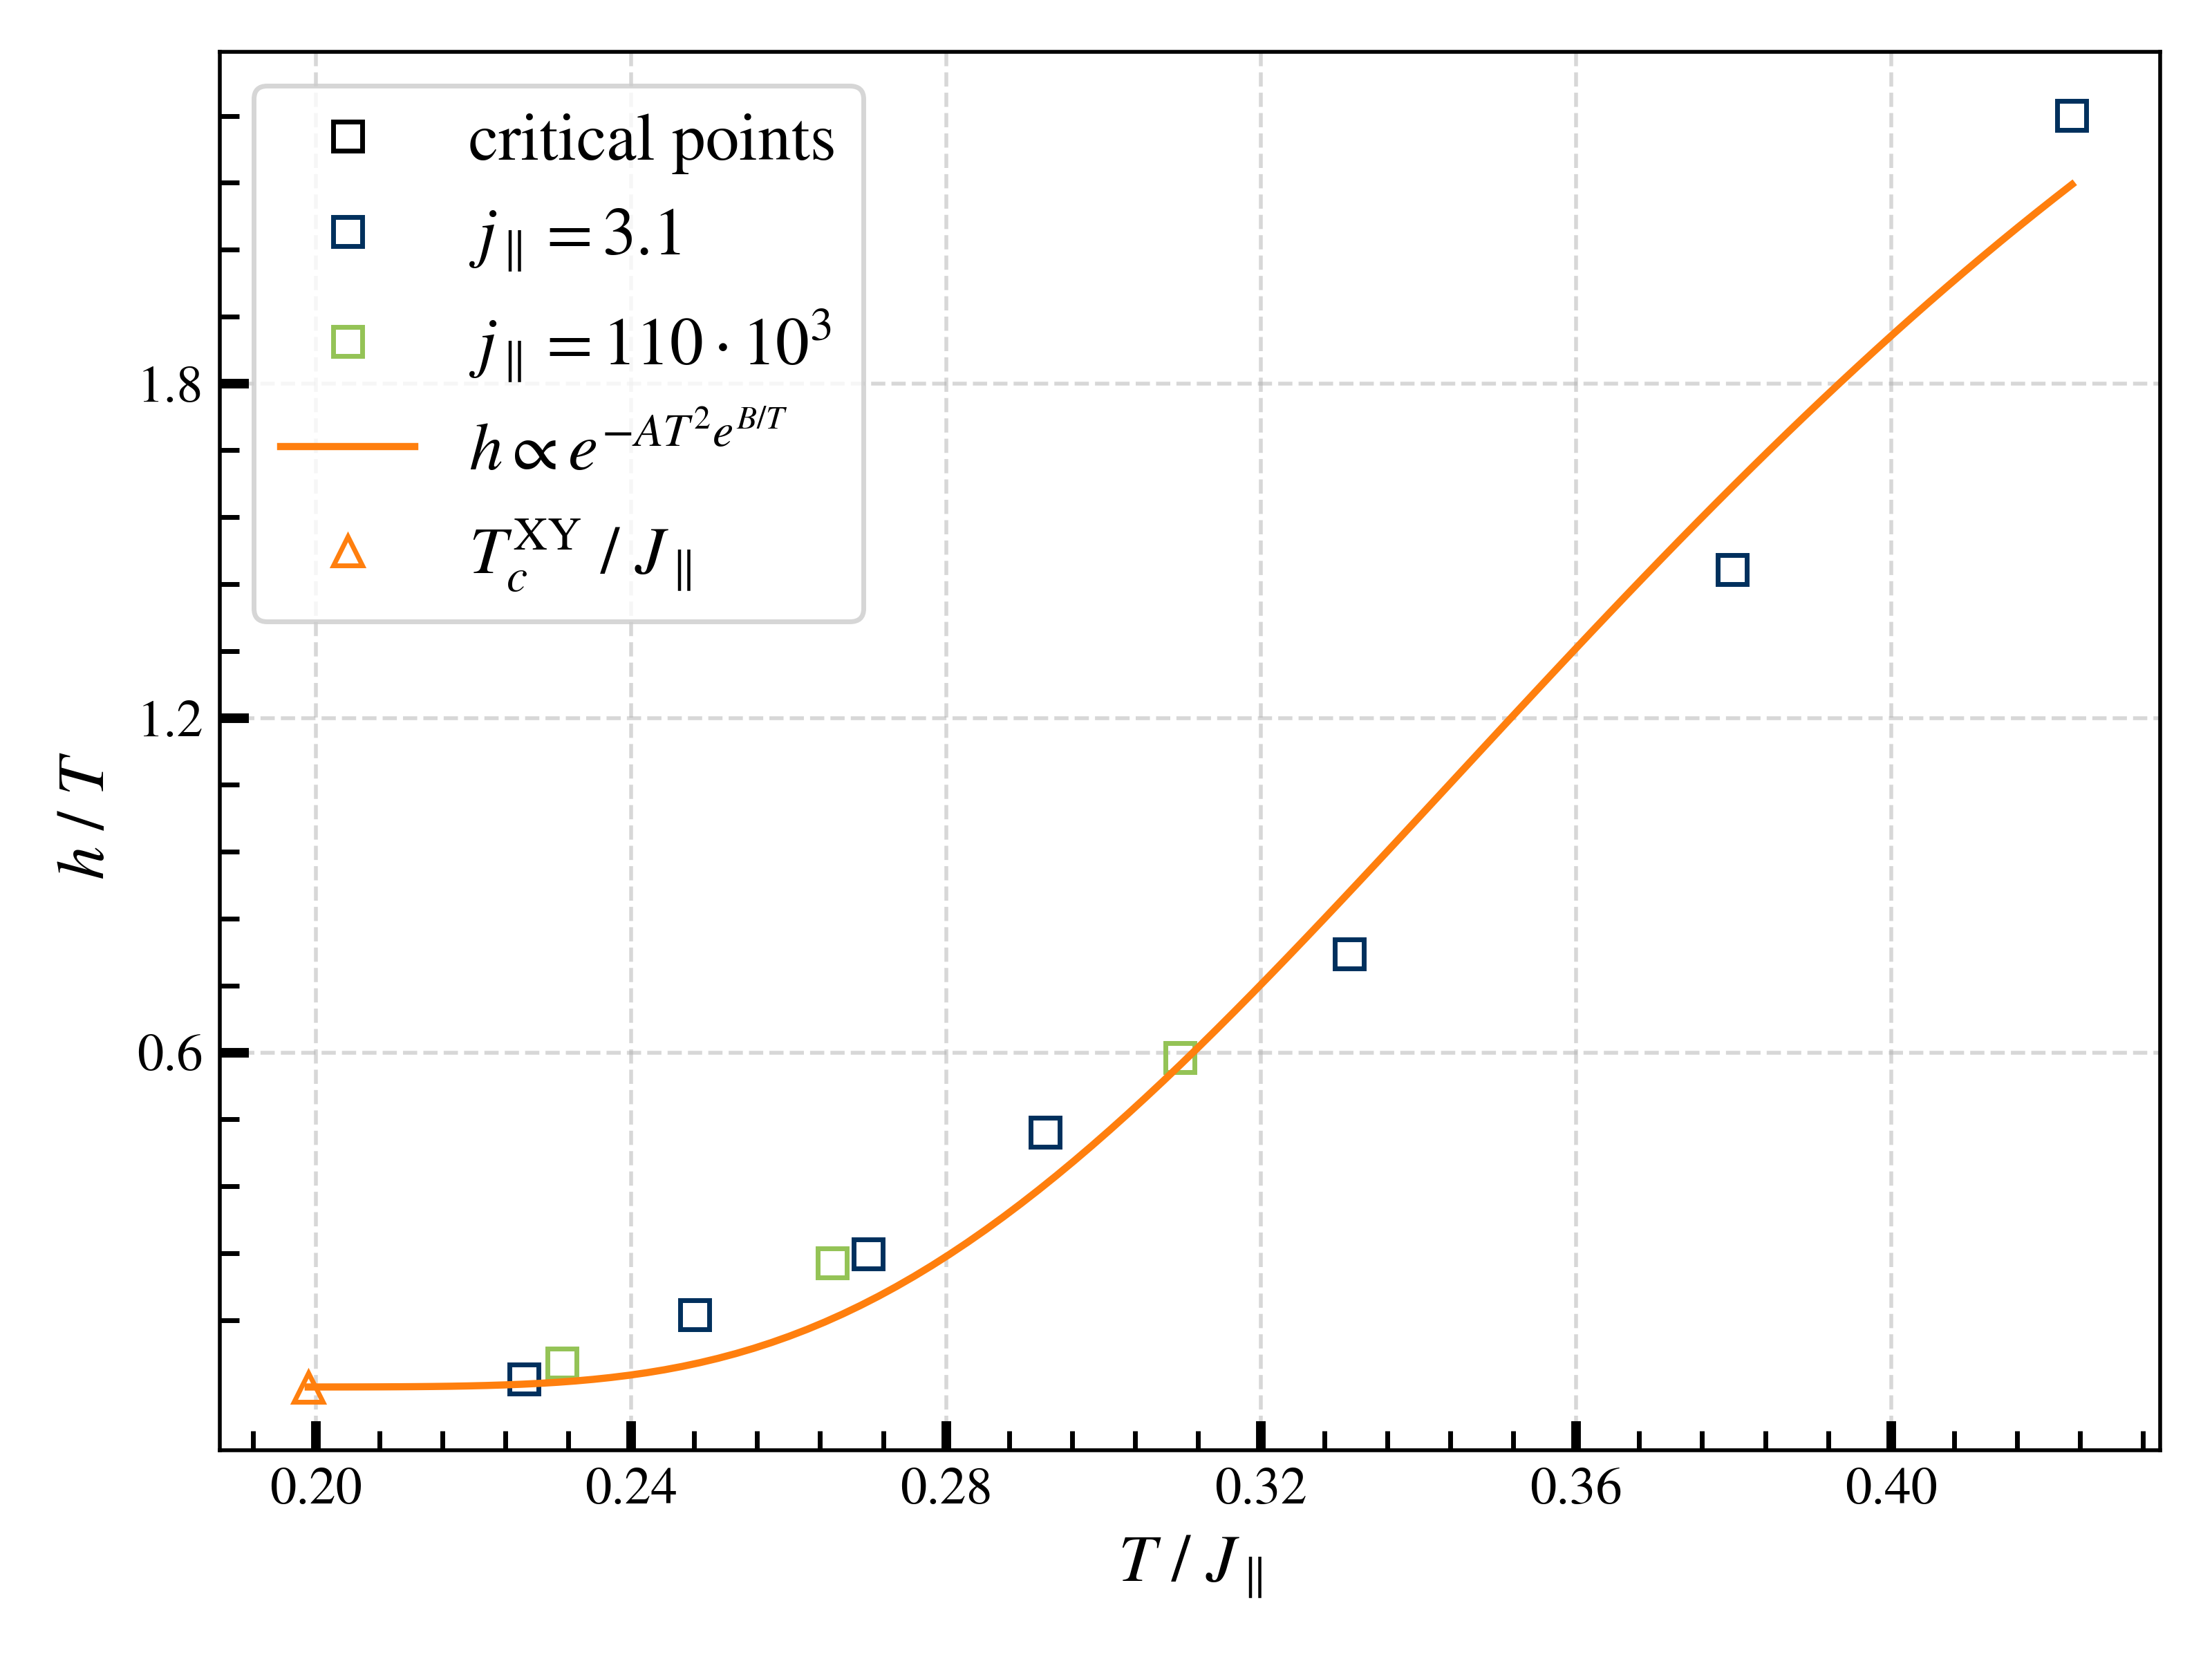
\includegraphics[width=0.9\linewidth]{graphics/phase_transition-h(T).png}
		\end{subfigure} \\
		\begin{subfigure}{0.9\textwidth}
			\centering
			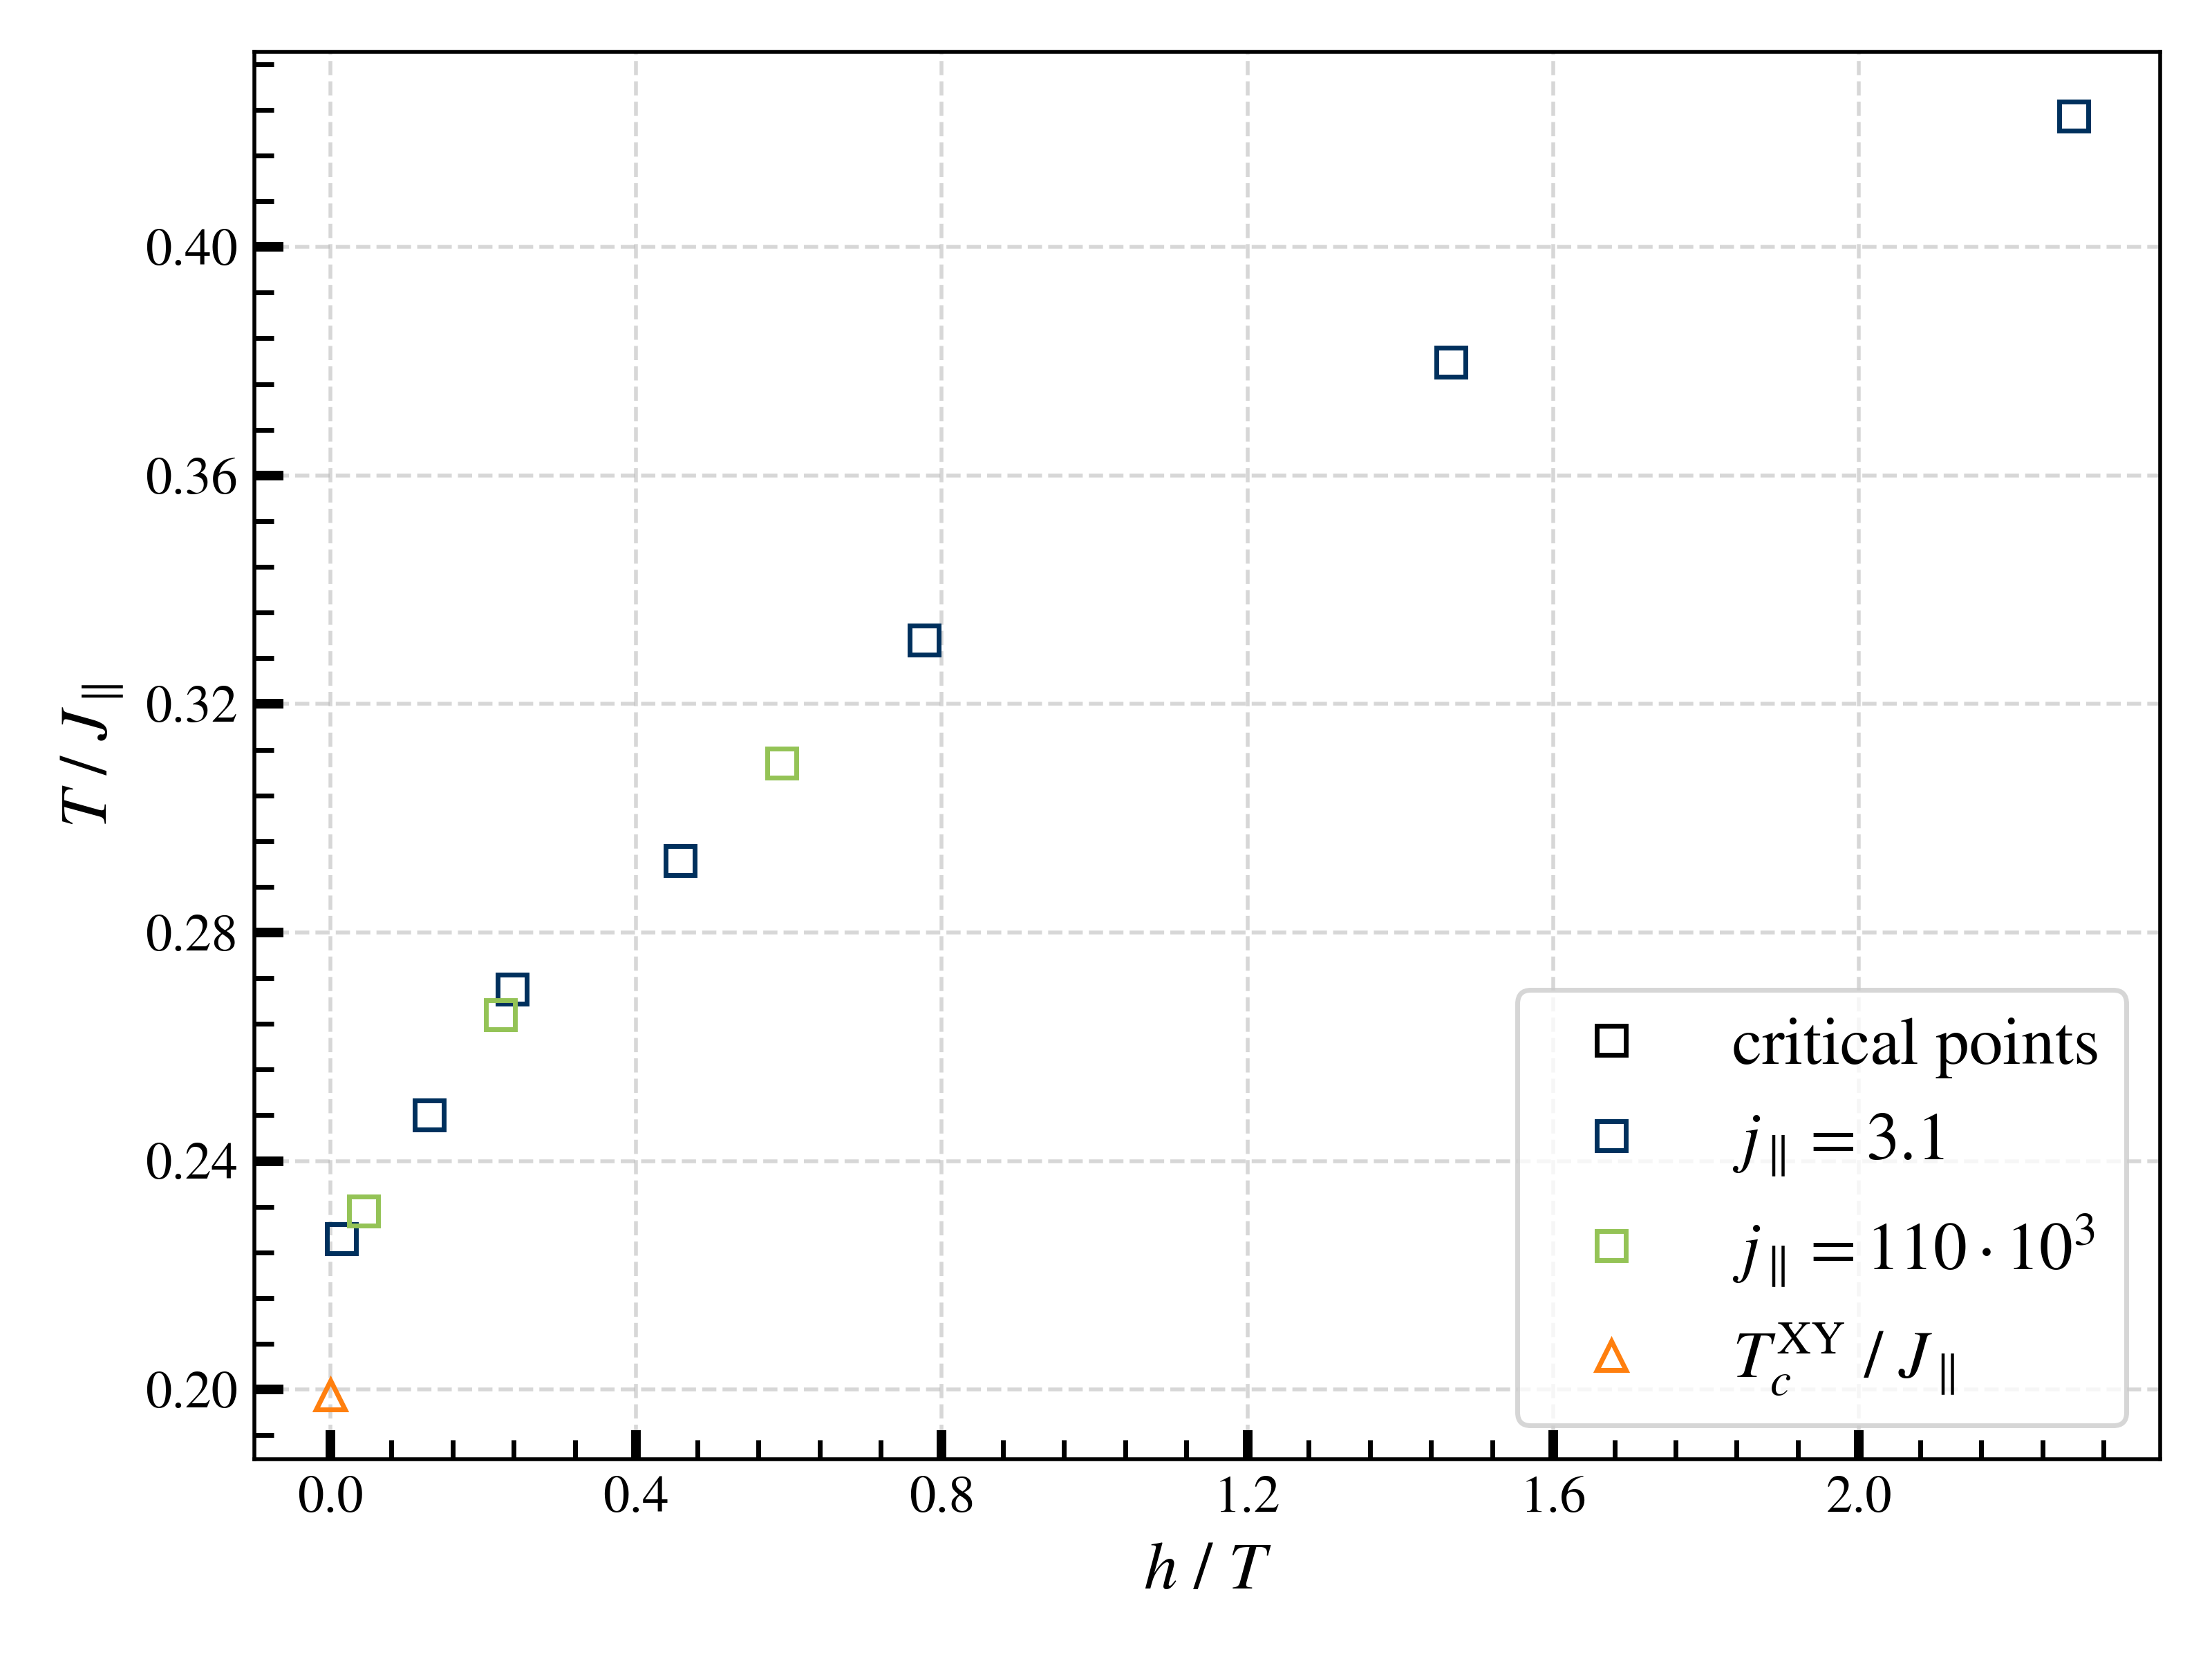
\includegraphics[width=0.92\linewidth]{graphics/phase_transition-T(h).png}
		\end{subfigure}
		\caption{Phase diagrams in the $\tfrac{T}{J_\parallel} - \tfrac{h}{T}-$plane are shown for $J_\parallel /	J_\perp =	31$. Curves for different absolute values of $j_\delta$ collapse when normalized as shown.  \textbf{(a)} The dependence  of critical symmetry breaking field $\beta h_c$ is plotted versus the effective temperature. The curve $\tfrac{h}{T} \left(\tfrac{T}{J_\parallel}\right)$ follows the expected behavior from \cite{jose1977renormalization}. A fit of $\tfrac{h}{T} \propto e^{-AT^2 \exp({B/T})}$ is shown in orange. For the constants we extract $A=0.909$ and $B=1.184$. \textbf{(b)} The inverse plot gives a feeling for the saturation of $T_c$. In both plots the critical temperature $T_c^{\text{XY}}$ of the isotropic XY model obtained from Eq.~\eqref{Eq::XY-crit-general-effective} is shown. (Question: Rather write $\beta h$ and $1 /	(\beta J_\parallel)$ ?)}
		\label{Fig::Phase-Diagram-h}
	\end{figure}
	\subsection{The Correlation Length Amplitudes $\boldsymbol{\xi_\delta^+}$}
	The static scaling law of the correlation length $\xi_\delta$ above the critical temperature ($\varepsilon > 0$) given by Eq.~\eqref{Eq::RG-xi-scaling} can be rewritten as
	\begin{equation} \label{Eq::Xi-divergence-amplitude}
		\xi_\delta (\varepsilon) = \xi_\delta^{+} \varepsilon^{-\nu}~,
	\end{equation}
	for anisotropic systems. The proportionality factors $\xi_\delta^{+}$ are called the correlation length amplitudes. The correlation lengths in the Ising model can be analytically expressed in terms of the temperature and the coupling constants $J_\delta$. Their relation above the critical temperature is given by Eq.~\eqref{Eq::Ising-Corrlength-Coupling}. An expansion of Eq.~ \eqref{Eq::Ising-Corrlength-Coupling} around $T_c$ leads to the expression
	\begin{equation} \label{Eq::Ising-Ampl-ratio-xi}
		\sinh \left(\frac{2 |J_\delta|}{k_B T_c}\right) =	\frac{\xi_\delta^+ / a_\delta}{\xi_{\overline{\delta}}^+ / a_{\overline{\delta}}}~.
	\end{equation}
	This relation is exceptionally useful, as it can be used to determine the coupling energies $J_\delta$ from the measured correlation lengths and critical temperature. The value that is this way obtained by Brand et. al \cite{brand2023dimer, brand2023critical} for the amplitude ratio in units of the lattice constants is $({\xi_\parallel^+ / a_\parallel}) \big/	({\xi_{\perp}^+ / a_{\perp}}) =	10.3$.  \\
	
	An expression like \eqref{Eq::Ising-Ampl-ratio-xi} for the anisotropic XY model is not known at the moment. Hence, a analytic relation of the correlation length ratio to the model couplings $J_\delta$ and $h$ is not possible. However, since the symmetry broken XY model and the Ising model have shown to behave quite similar in the previous investigations, it is reasonable to examine the correlation length amplitude ratio for the Ising coupling constant ratio $J_\parallel /	J_\perp \approx	30$. To extract $\xi^+_\delta$, the scaling of $\xi_\delta^{-1}$ is considered, which is given by
	\begin{equation} \label{Eq::inv-divergence-fit}
		\xi_\delta^{-1}(T) =	\frac{1}{\xi_\delta^+} \left(\frac{T - T_c}{T_c}\right) =	- \frac{1}{\xi_\delta^+} + (T_c \xi_\delta^+)^{-1} T ~,
	\end{equation}
	using the result $\nu =	1$. Therefore $\xi$ behaves linearly in $T$ around the critical point.\\
	
	The amplitude ratio is investigated by preparing the system in a random state and letting it relax at a fixed temperatures $T \gtrsim T_c$. To judge whether the system is relaxed and at the same time obtain a precise value for the equilibrium correlation length, $\xi$ is monitored on the run like described in \autoref{Section::observable-measurement}. The extraction of the correlation length is for the XY model is described in \autoref{Section::Corr-Length-Calculation}. The chosen system sizes are large to minimize finite size effects. They are increased from $L_\parallel =	1024$ to $L_\parallel =	4096$ as $T_c$ is approached. \\

	The results are shown in \autoref{Fig::Amplitude-Result}. \autoref{Fig::Amplitude-Result} (a) and (d) show the correlation length and its inverse for $J_\parallel /	J_\perp =	30$ and $\beta_c h \approx 0.5$. The correlation length ratio of $\xi_\parallel^+ /   \xi_\perp^+ = 5.1 $ is smaller than expected for the Ising model. Reasons for this could be influences of the symmetry breaking field or just structural differences in the relationship of the coupling constants and the correlation lengths. To investigate the influence of $h$ on the $\xi_\parallel^+ /   \xi_\perp^+$, the measurement is repeated with $\beta_c h \approx 0.1$. \autoref{Fig::Amplitude-Result} (a) and (d) show that the quantitative values of the amplitudes change, but the ratio stays virtually the same. More measurements are needed to exclude a dependence of $\xi^+_\parallel /	\xi^+_\perp$ on $\beta_c h$. However, a strong dependency can already be ruled out. \\
	
	To approach the experimental ratio of $\xi_\parallel^+ /	\xi_\perp^+ \approx 10.3$, a simulation with $J_\parallel /	J_\perp =	100$ is performed. The results, shown in \autoref{Fig::Amplitude-Result} (c) and (d), have an amplitude ratio of $\xi_{\parallel}^+ /	\xi_\perp^+  \approx  8.9$. Although this is still smaller than the experimental ratio, this ratio shall be satisfying for the following measurements. After all, this is just a rough model and the experimental values are also not exact. \\
	
	\textcolor{red}{(Close to $T_c$ finite size effects become visible. To illustrate this, $\xi$ is recalculated at the questionable data points for a system of size $L_\parallel' =	2 L_\parallel$.)}
	
	Note that, when changing the ratio of $J_\parallel /	J_\perp$, we effectively move in the four dimensional phase space of our model, which \autoref{Fig::Phase-Diagram-h} is a cross section of. \autoref{Fig::Phase-Diagram-h} can therefore not be used to estimate the transition temperatures of the new ratio. We can however, guess the qualitative behavior. The effective critical temperature of the isotropic XY model for $J_\parallel /	J_\perp = 100$ is
	\begin{equation}
		T_c^{\text{XY}} /	J_\parallel =	0.148~.
	\end{equation}
	So the starting point in \autoref{Fig::Phase-Diagram-h} (b) is lower. We expect that the qualitative behavior is essentially the same, so one can get a rough picture of the new critical temperature by subtracting the differences of the XY model critical temperatures.
	
	\begin{figure}[htp]
		\begin{subfigure}{0.475\textwidth}
			\centering
			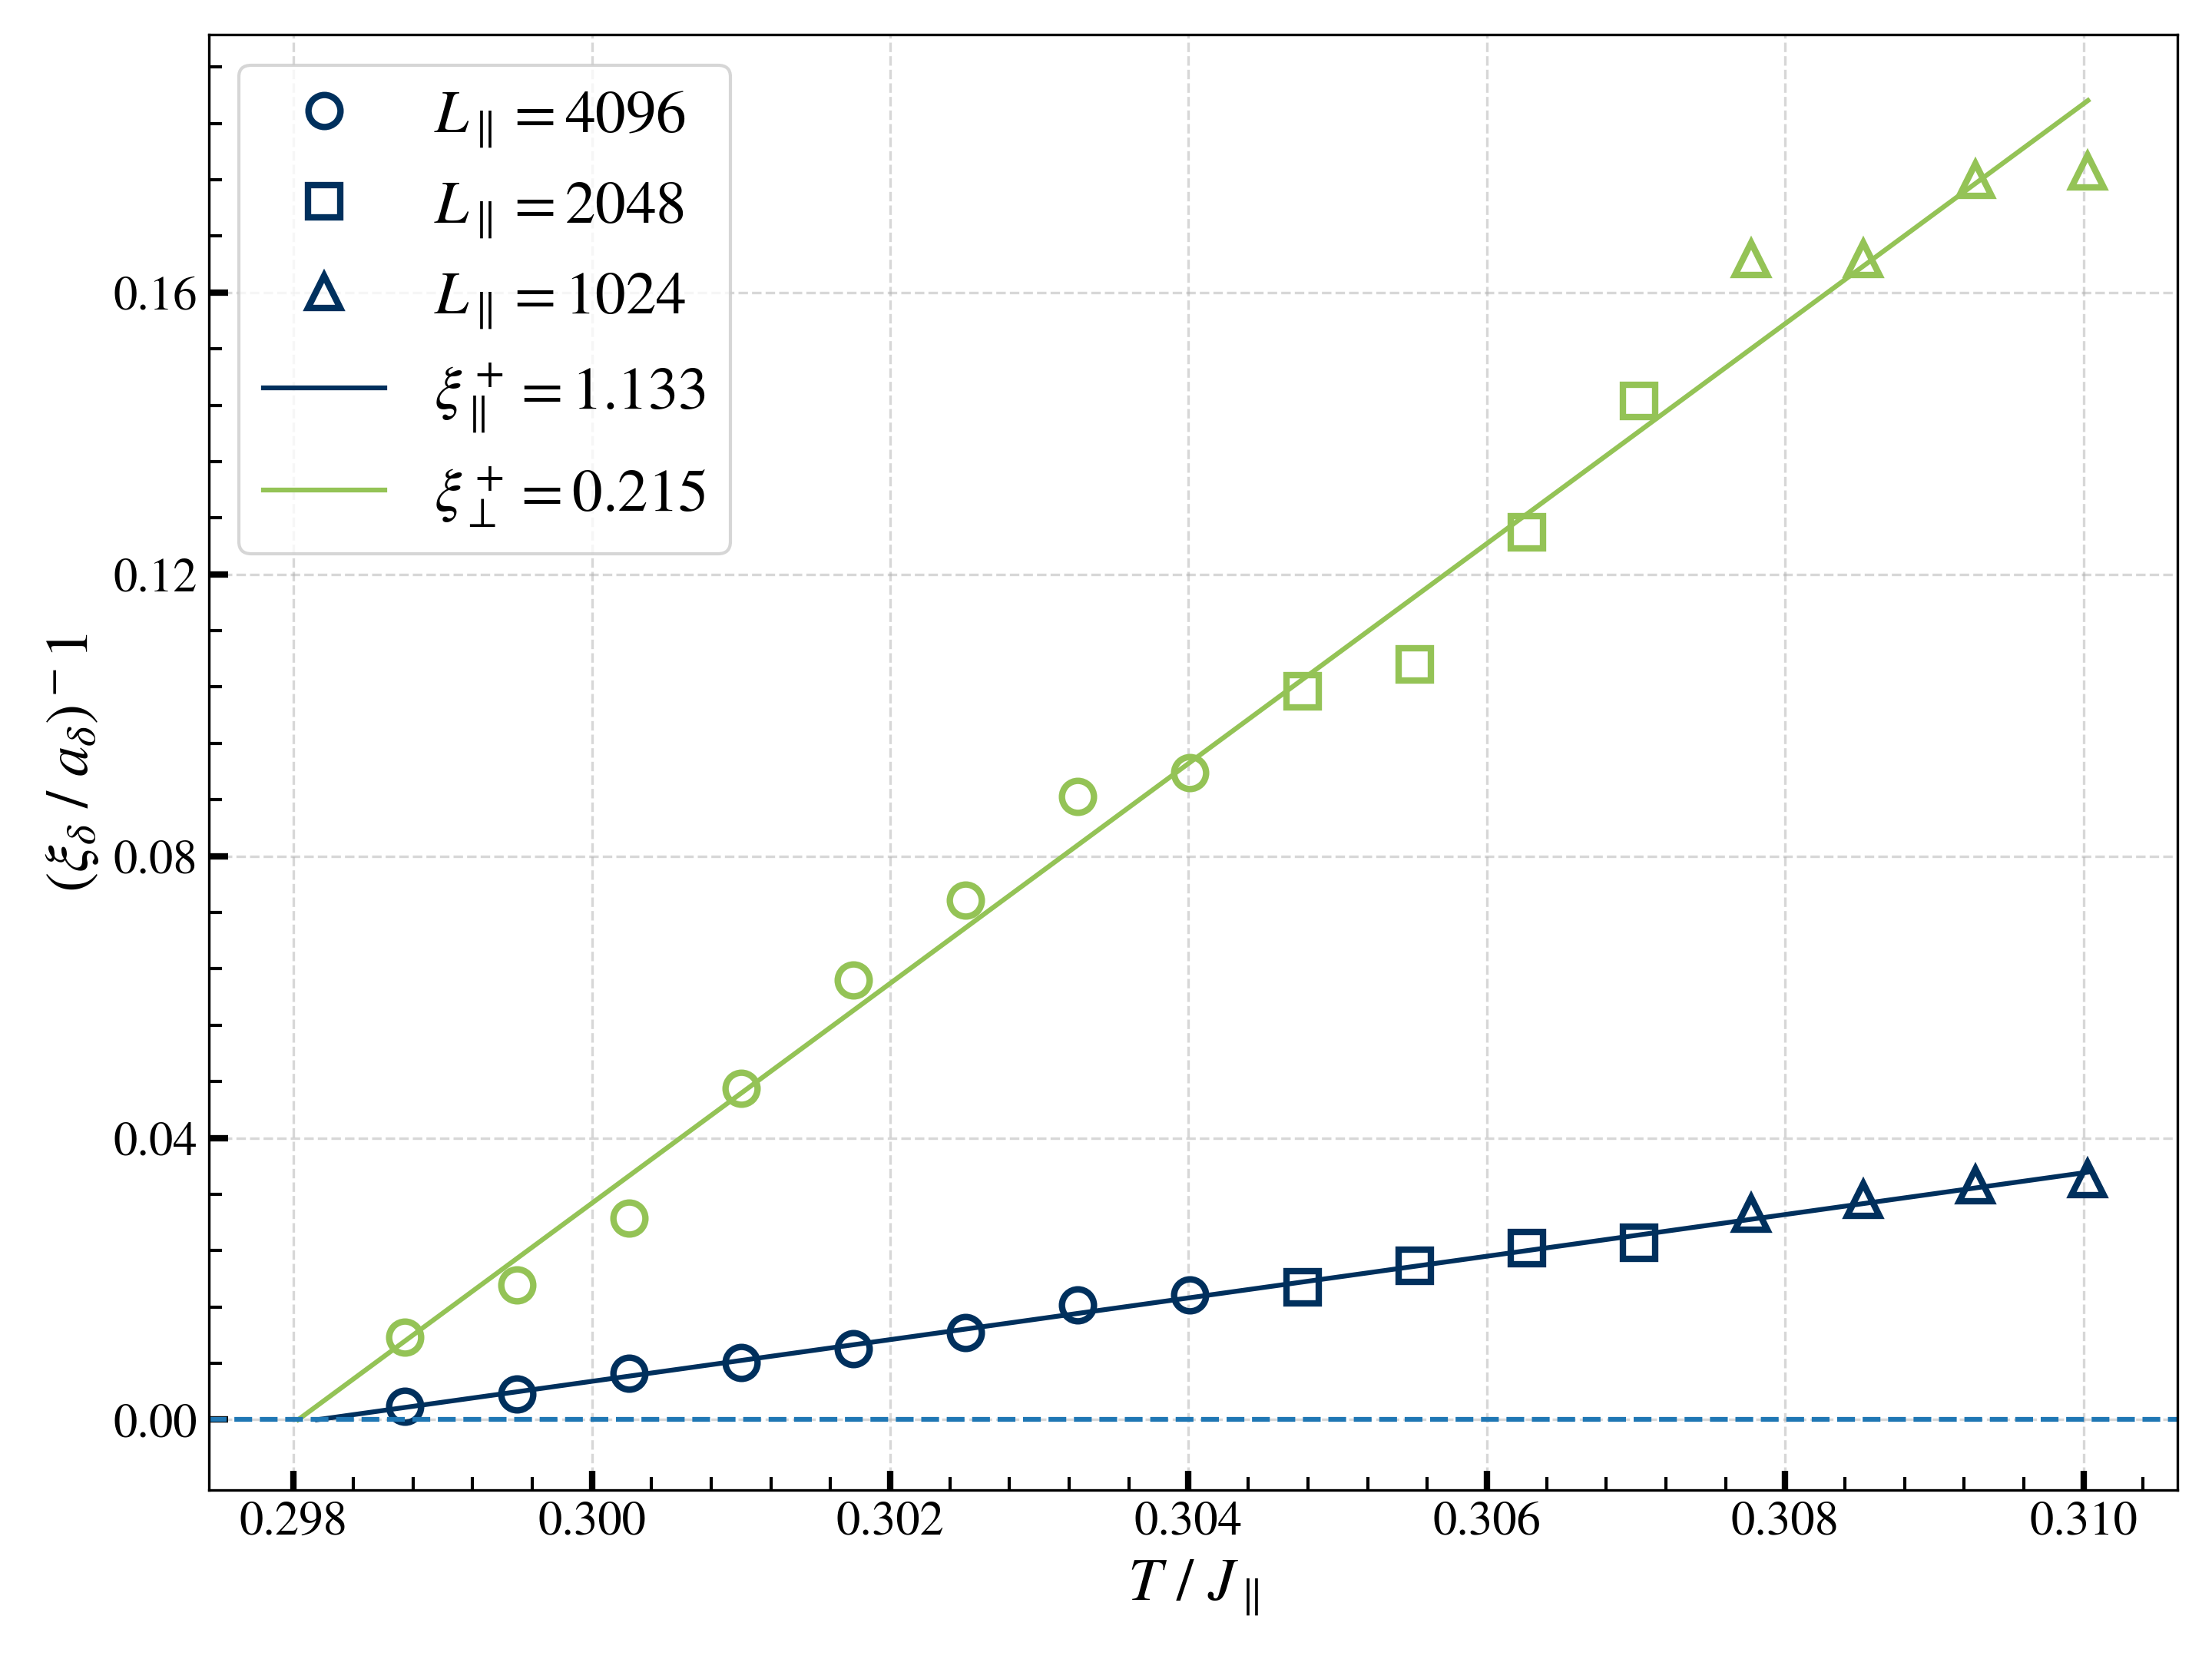
\includegraphics[width=0.95\linewidth]{graphics/xi-inv-divergence-30-3.png}
		\end{subfigure}
		\begin{subfigure}{0.475\textwidth}
			\centering
			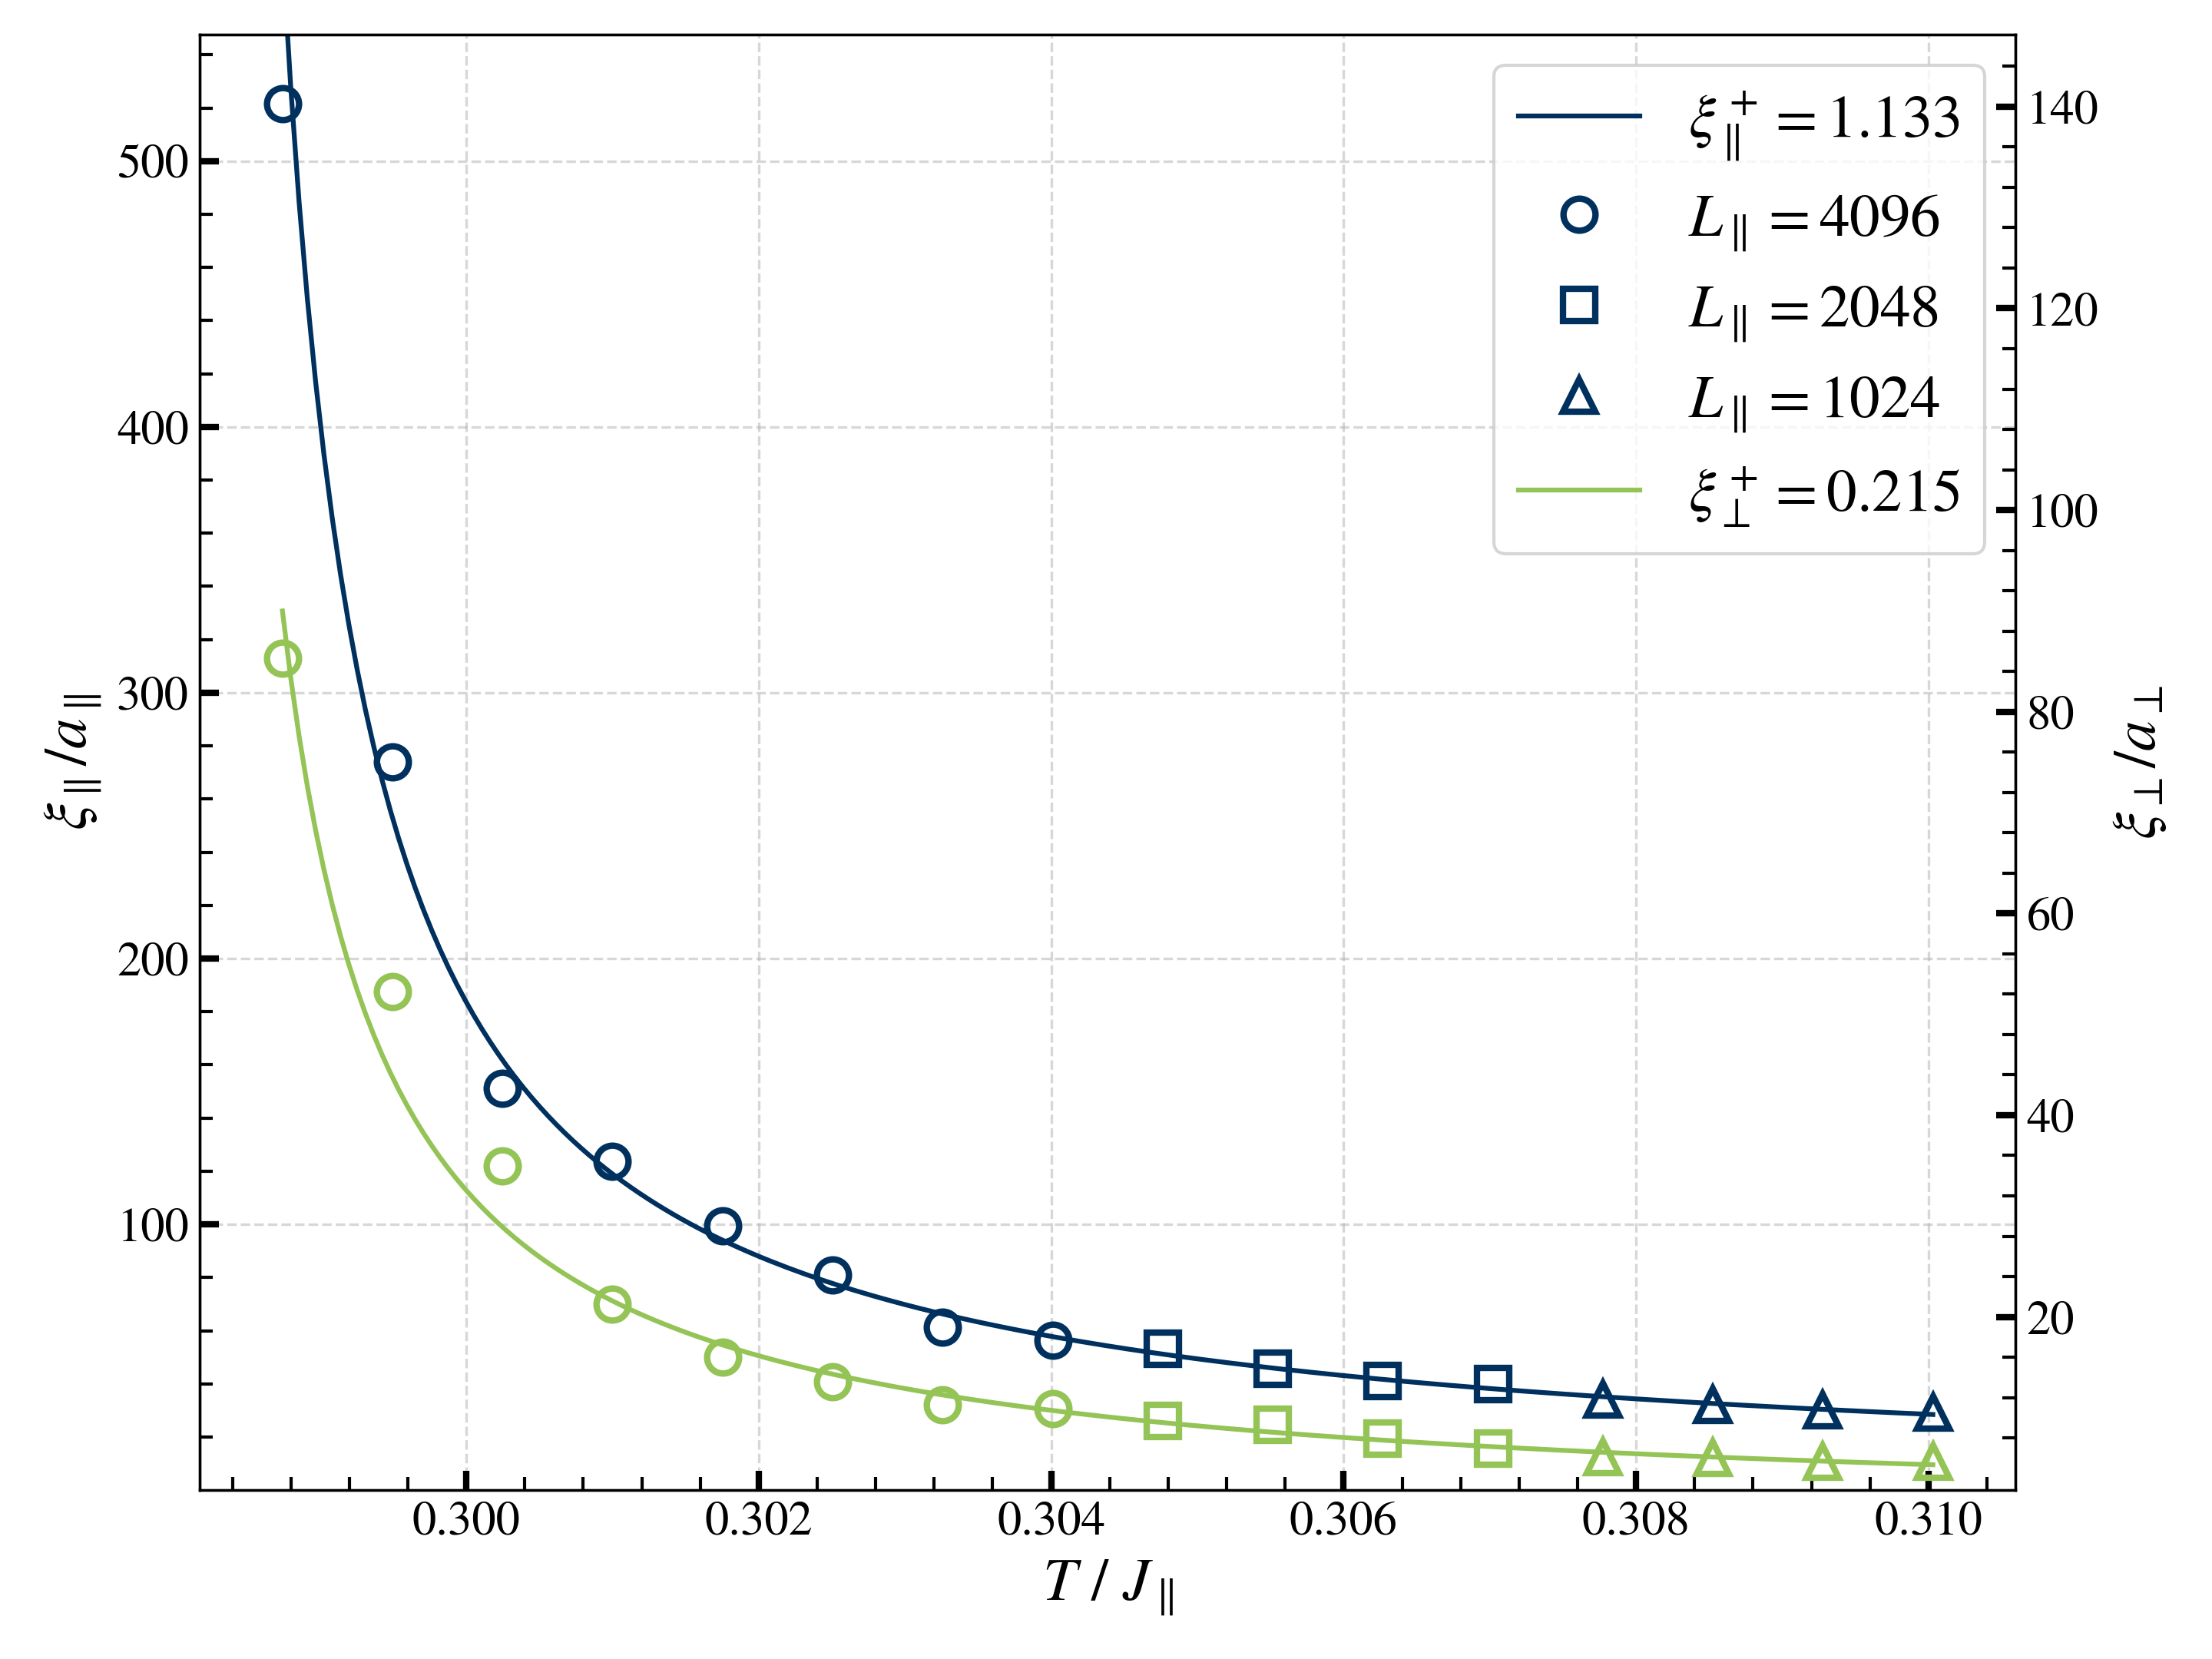
\includegraphics[width=0.95\linewidth]{graphics/xi-divergence-30-3.png}
		\end{subfigure} \\ 
		\begin{subfigure}{0.475\textwidth}
			\centering			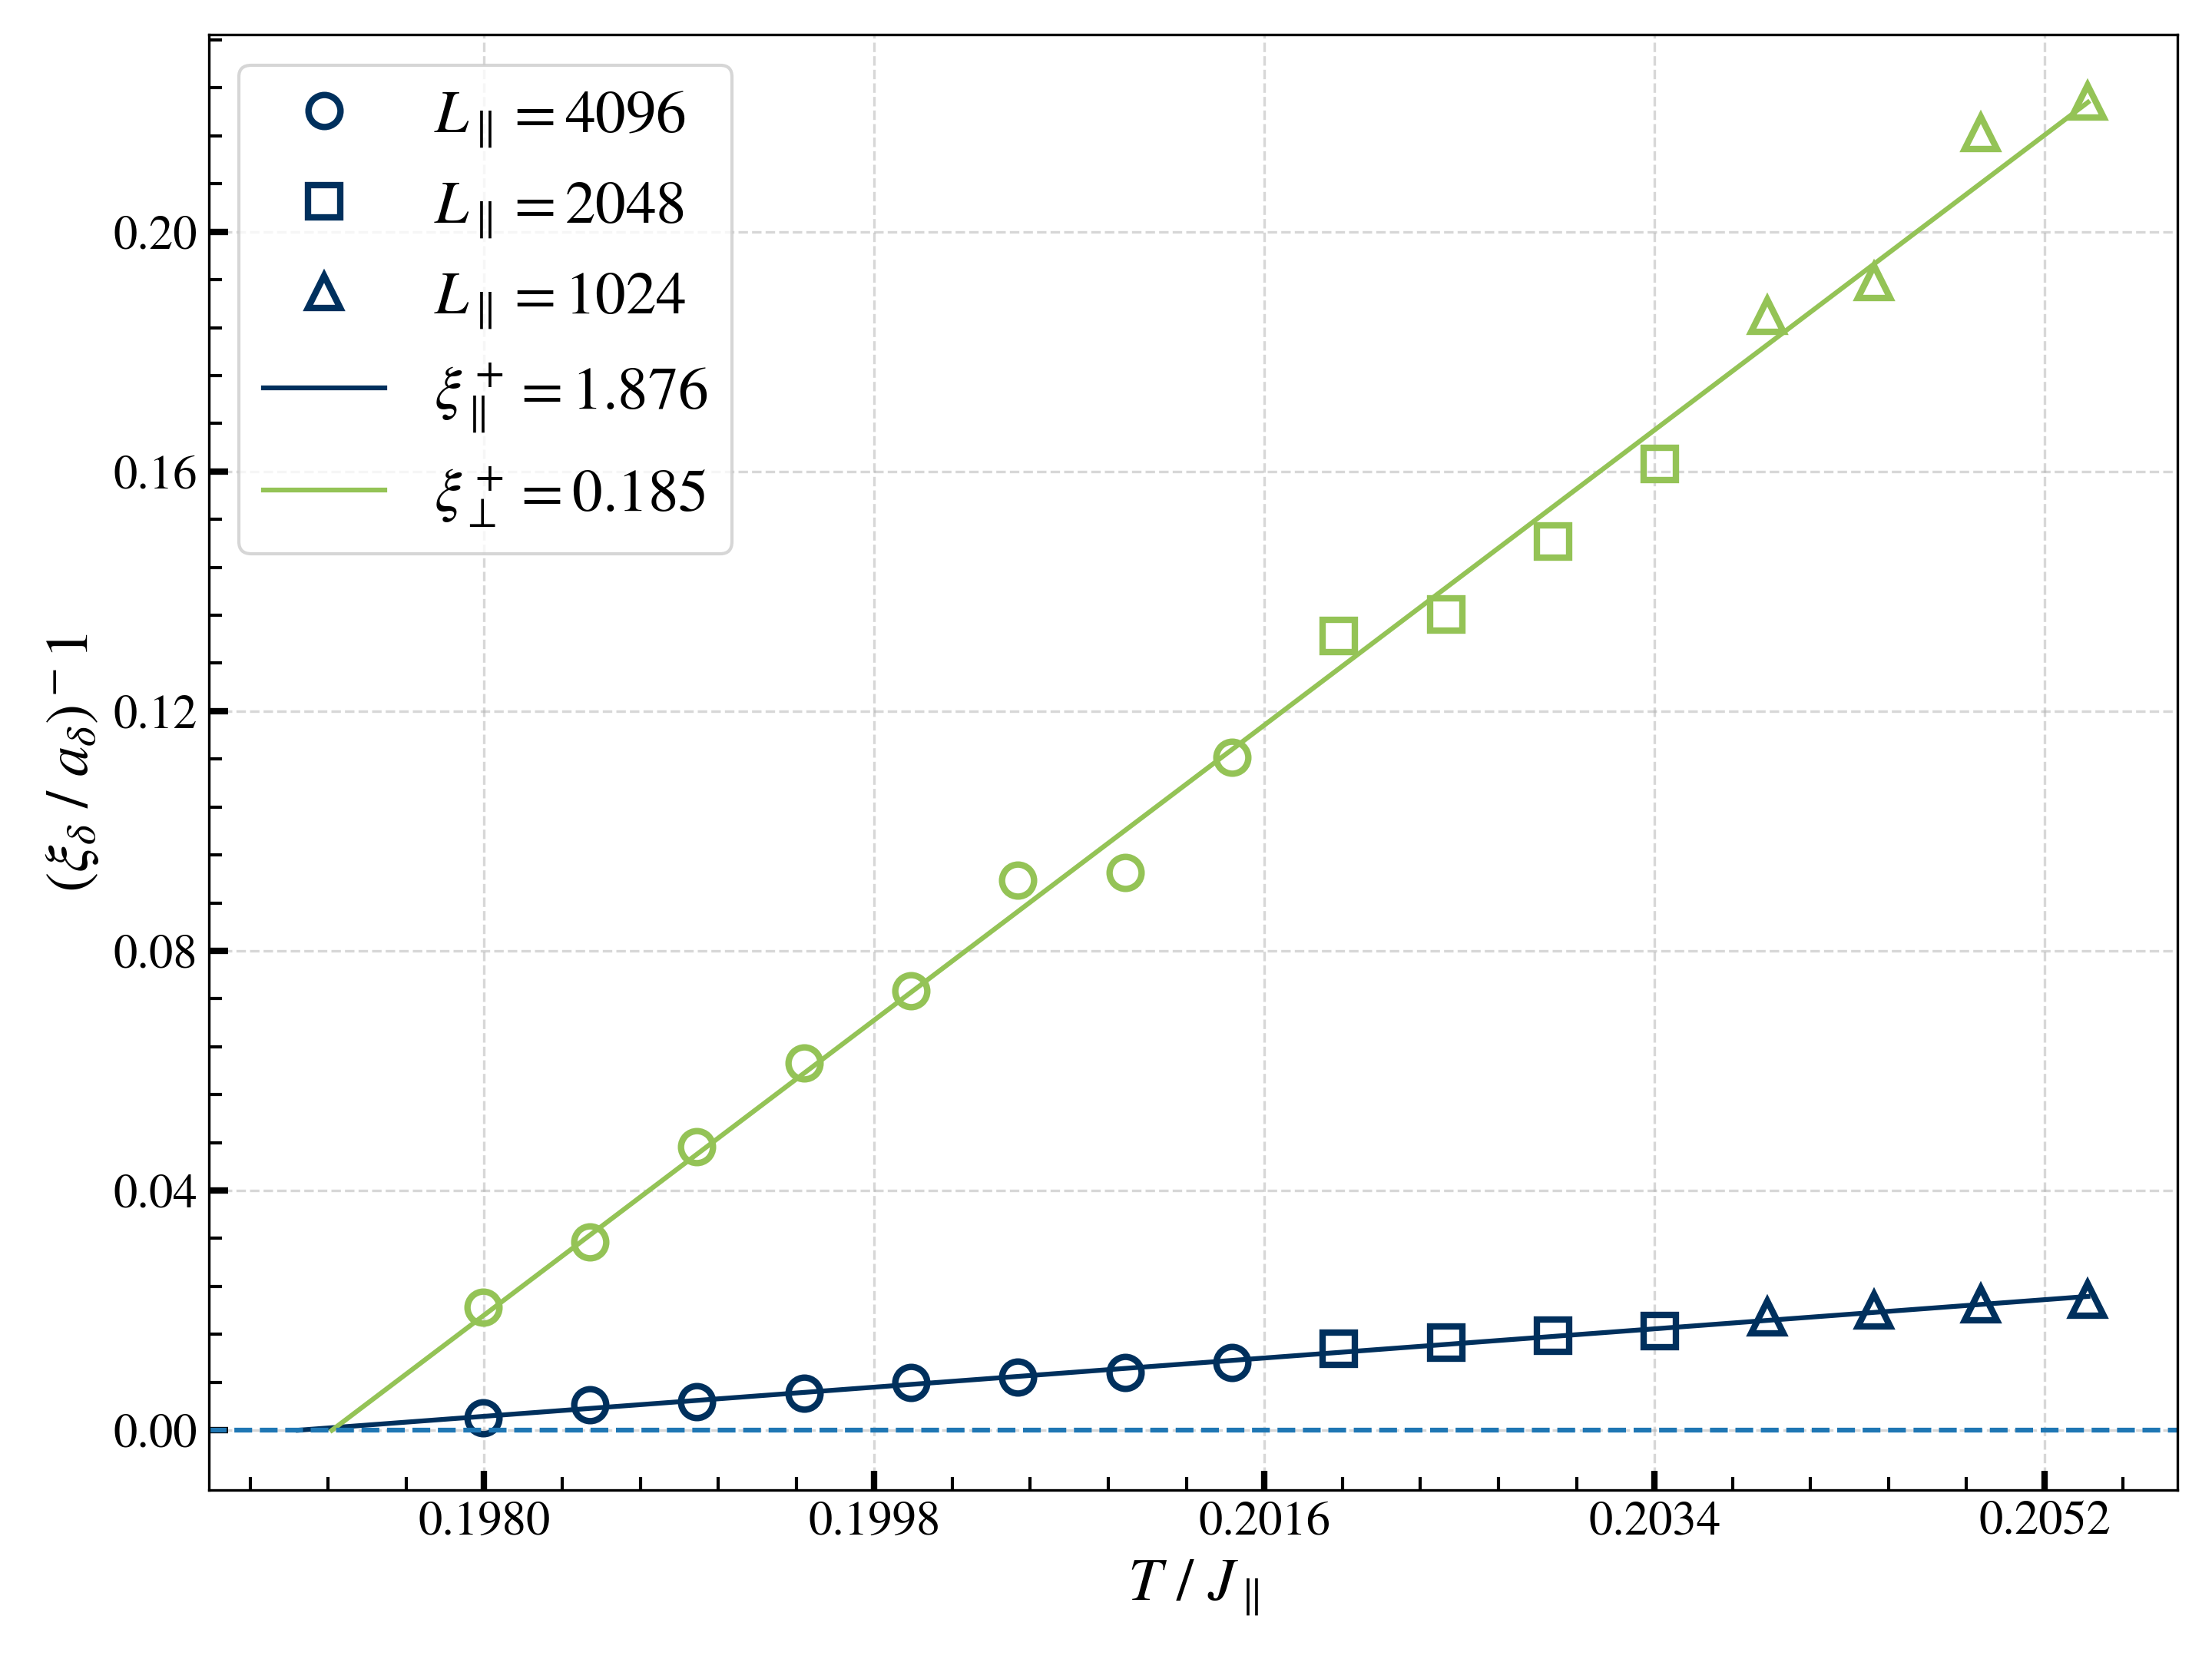
\includegraphics[width=0.95\linewidth]{graphics/xi-inv-divergence-100-3.png}
		\end{subfigure}
		\begin{subfigure}{0.475\textwidth}
			\centering			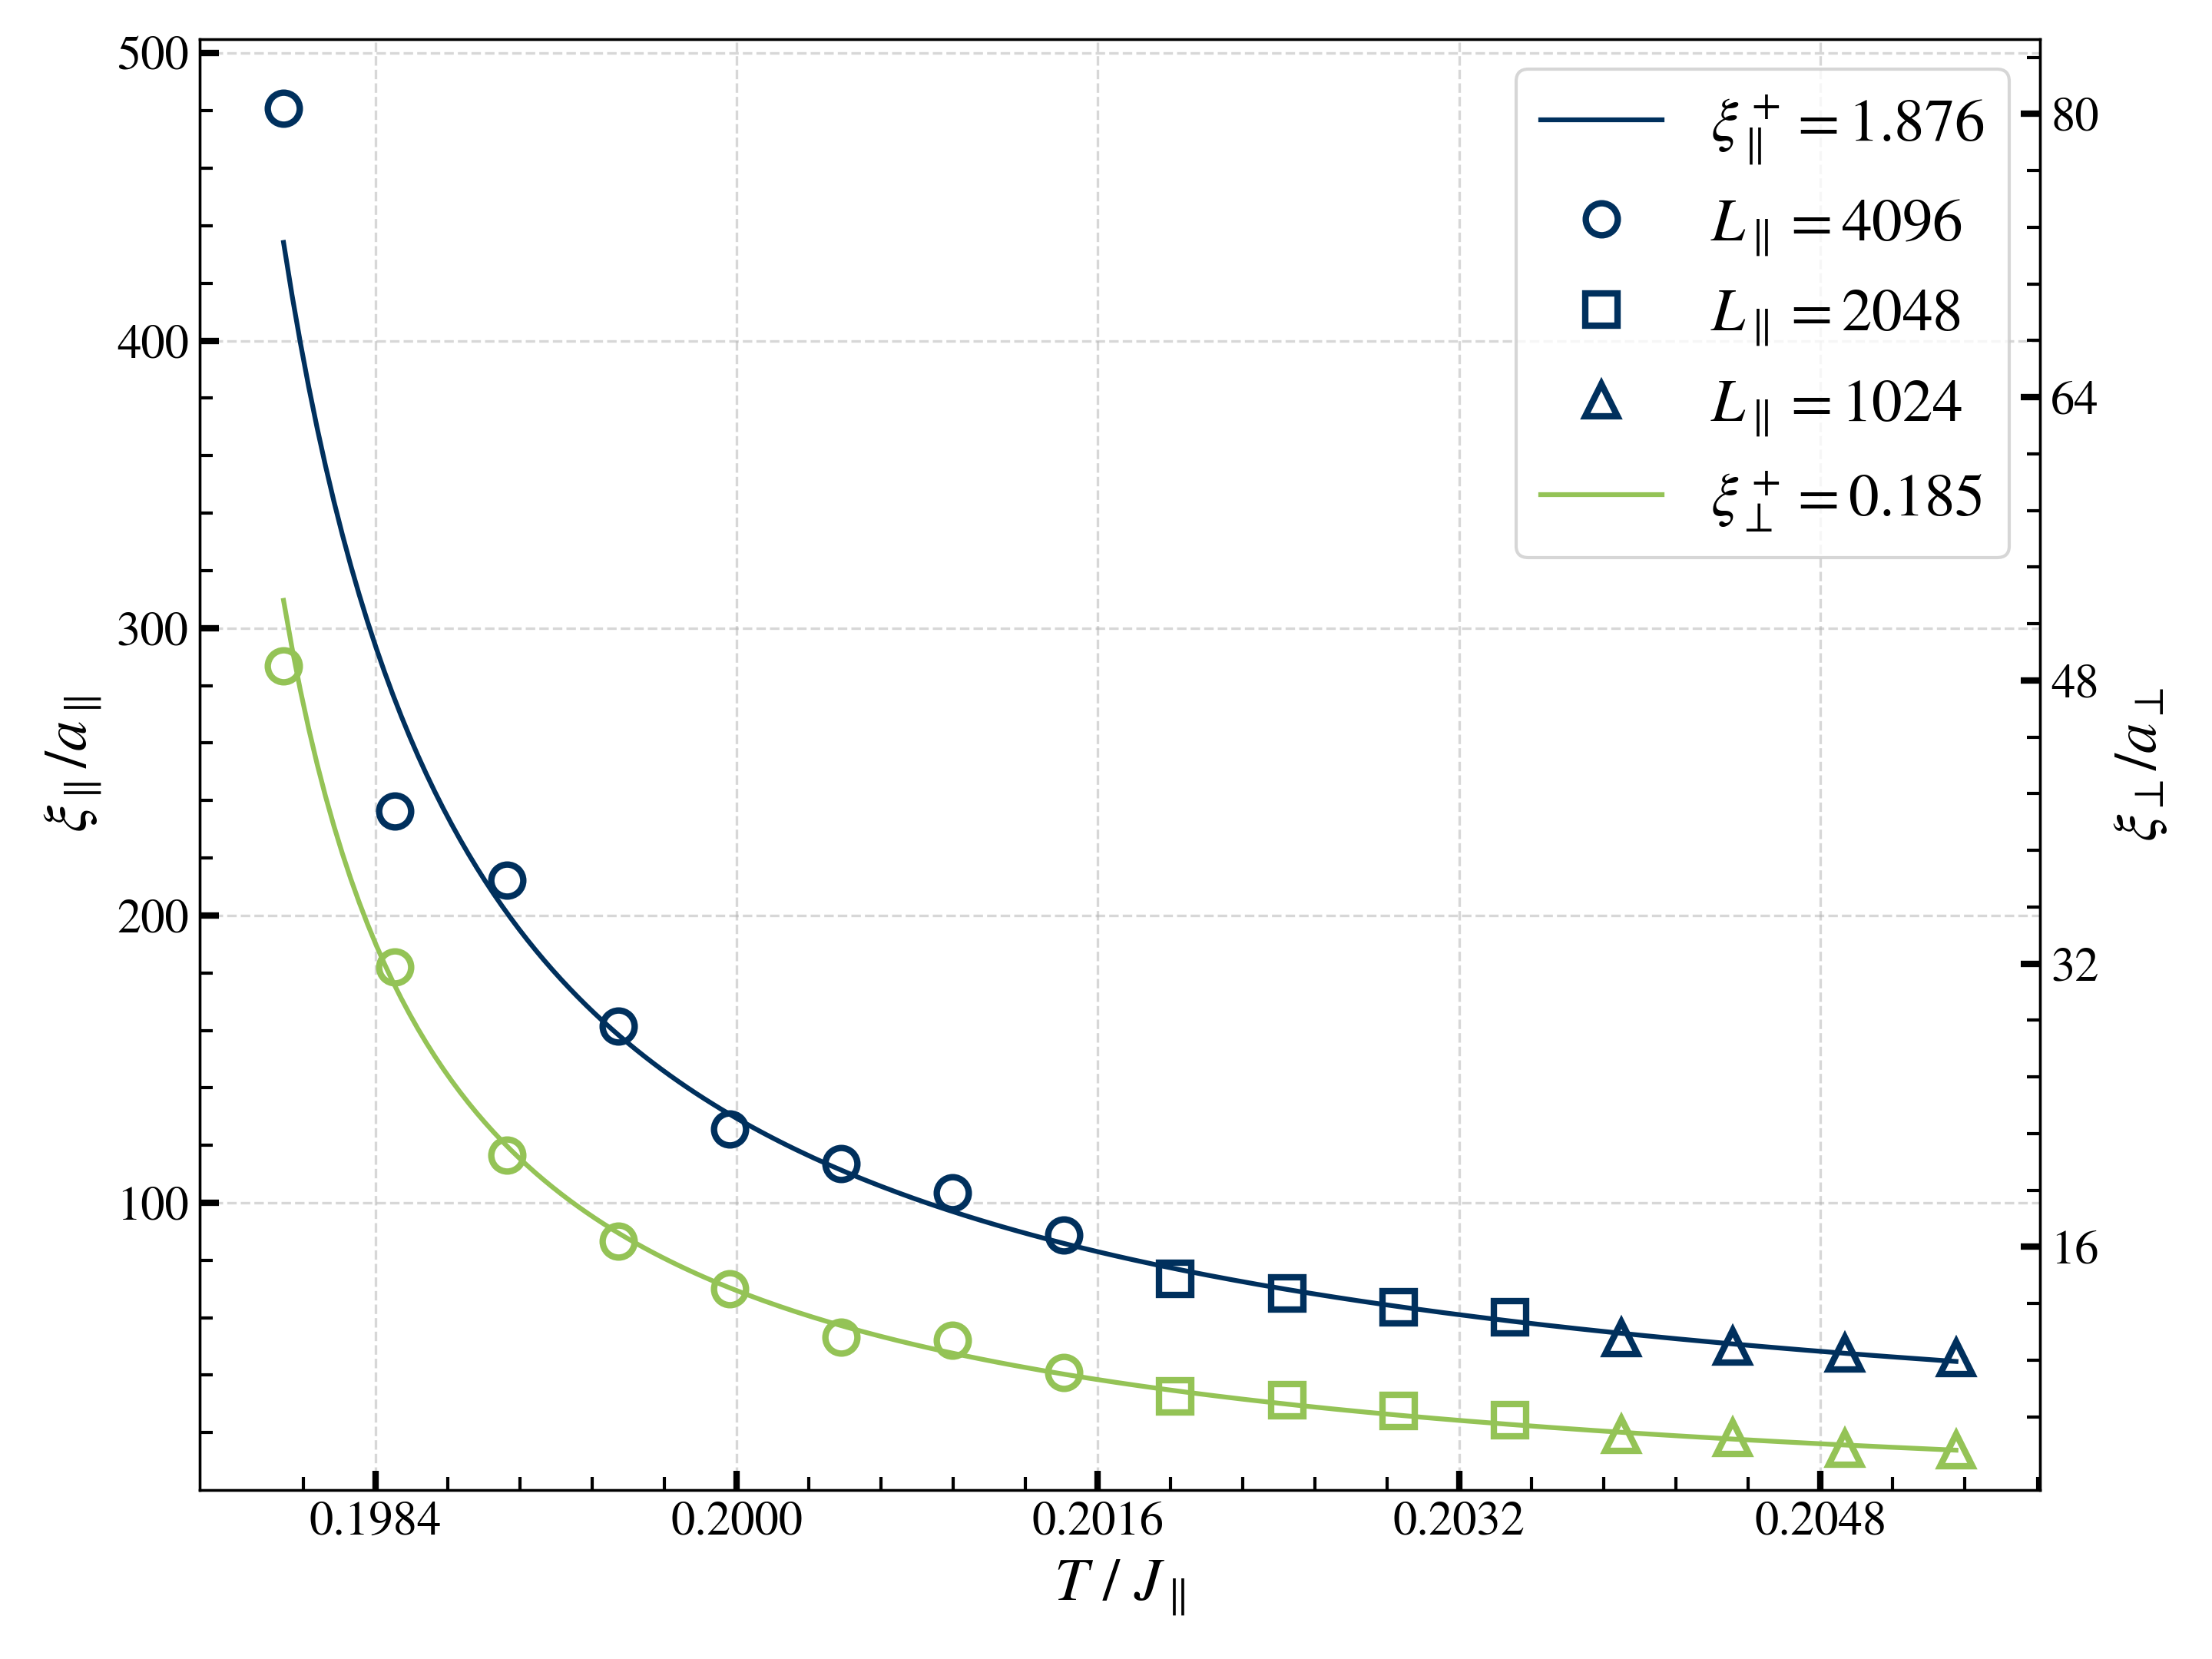
\includegraphics[width=0.95\linewidth]{graphics/xi-divergence-100-3.png}
		\end{subfigure} \\ 
		\begin{subfigure}{0.475\textwidth}
			\centering		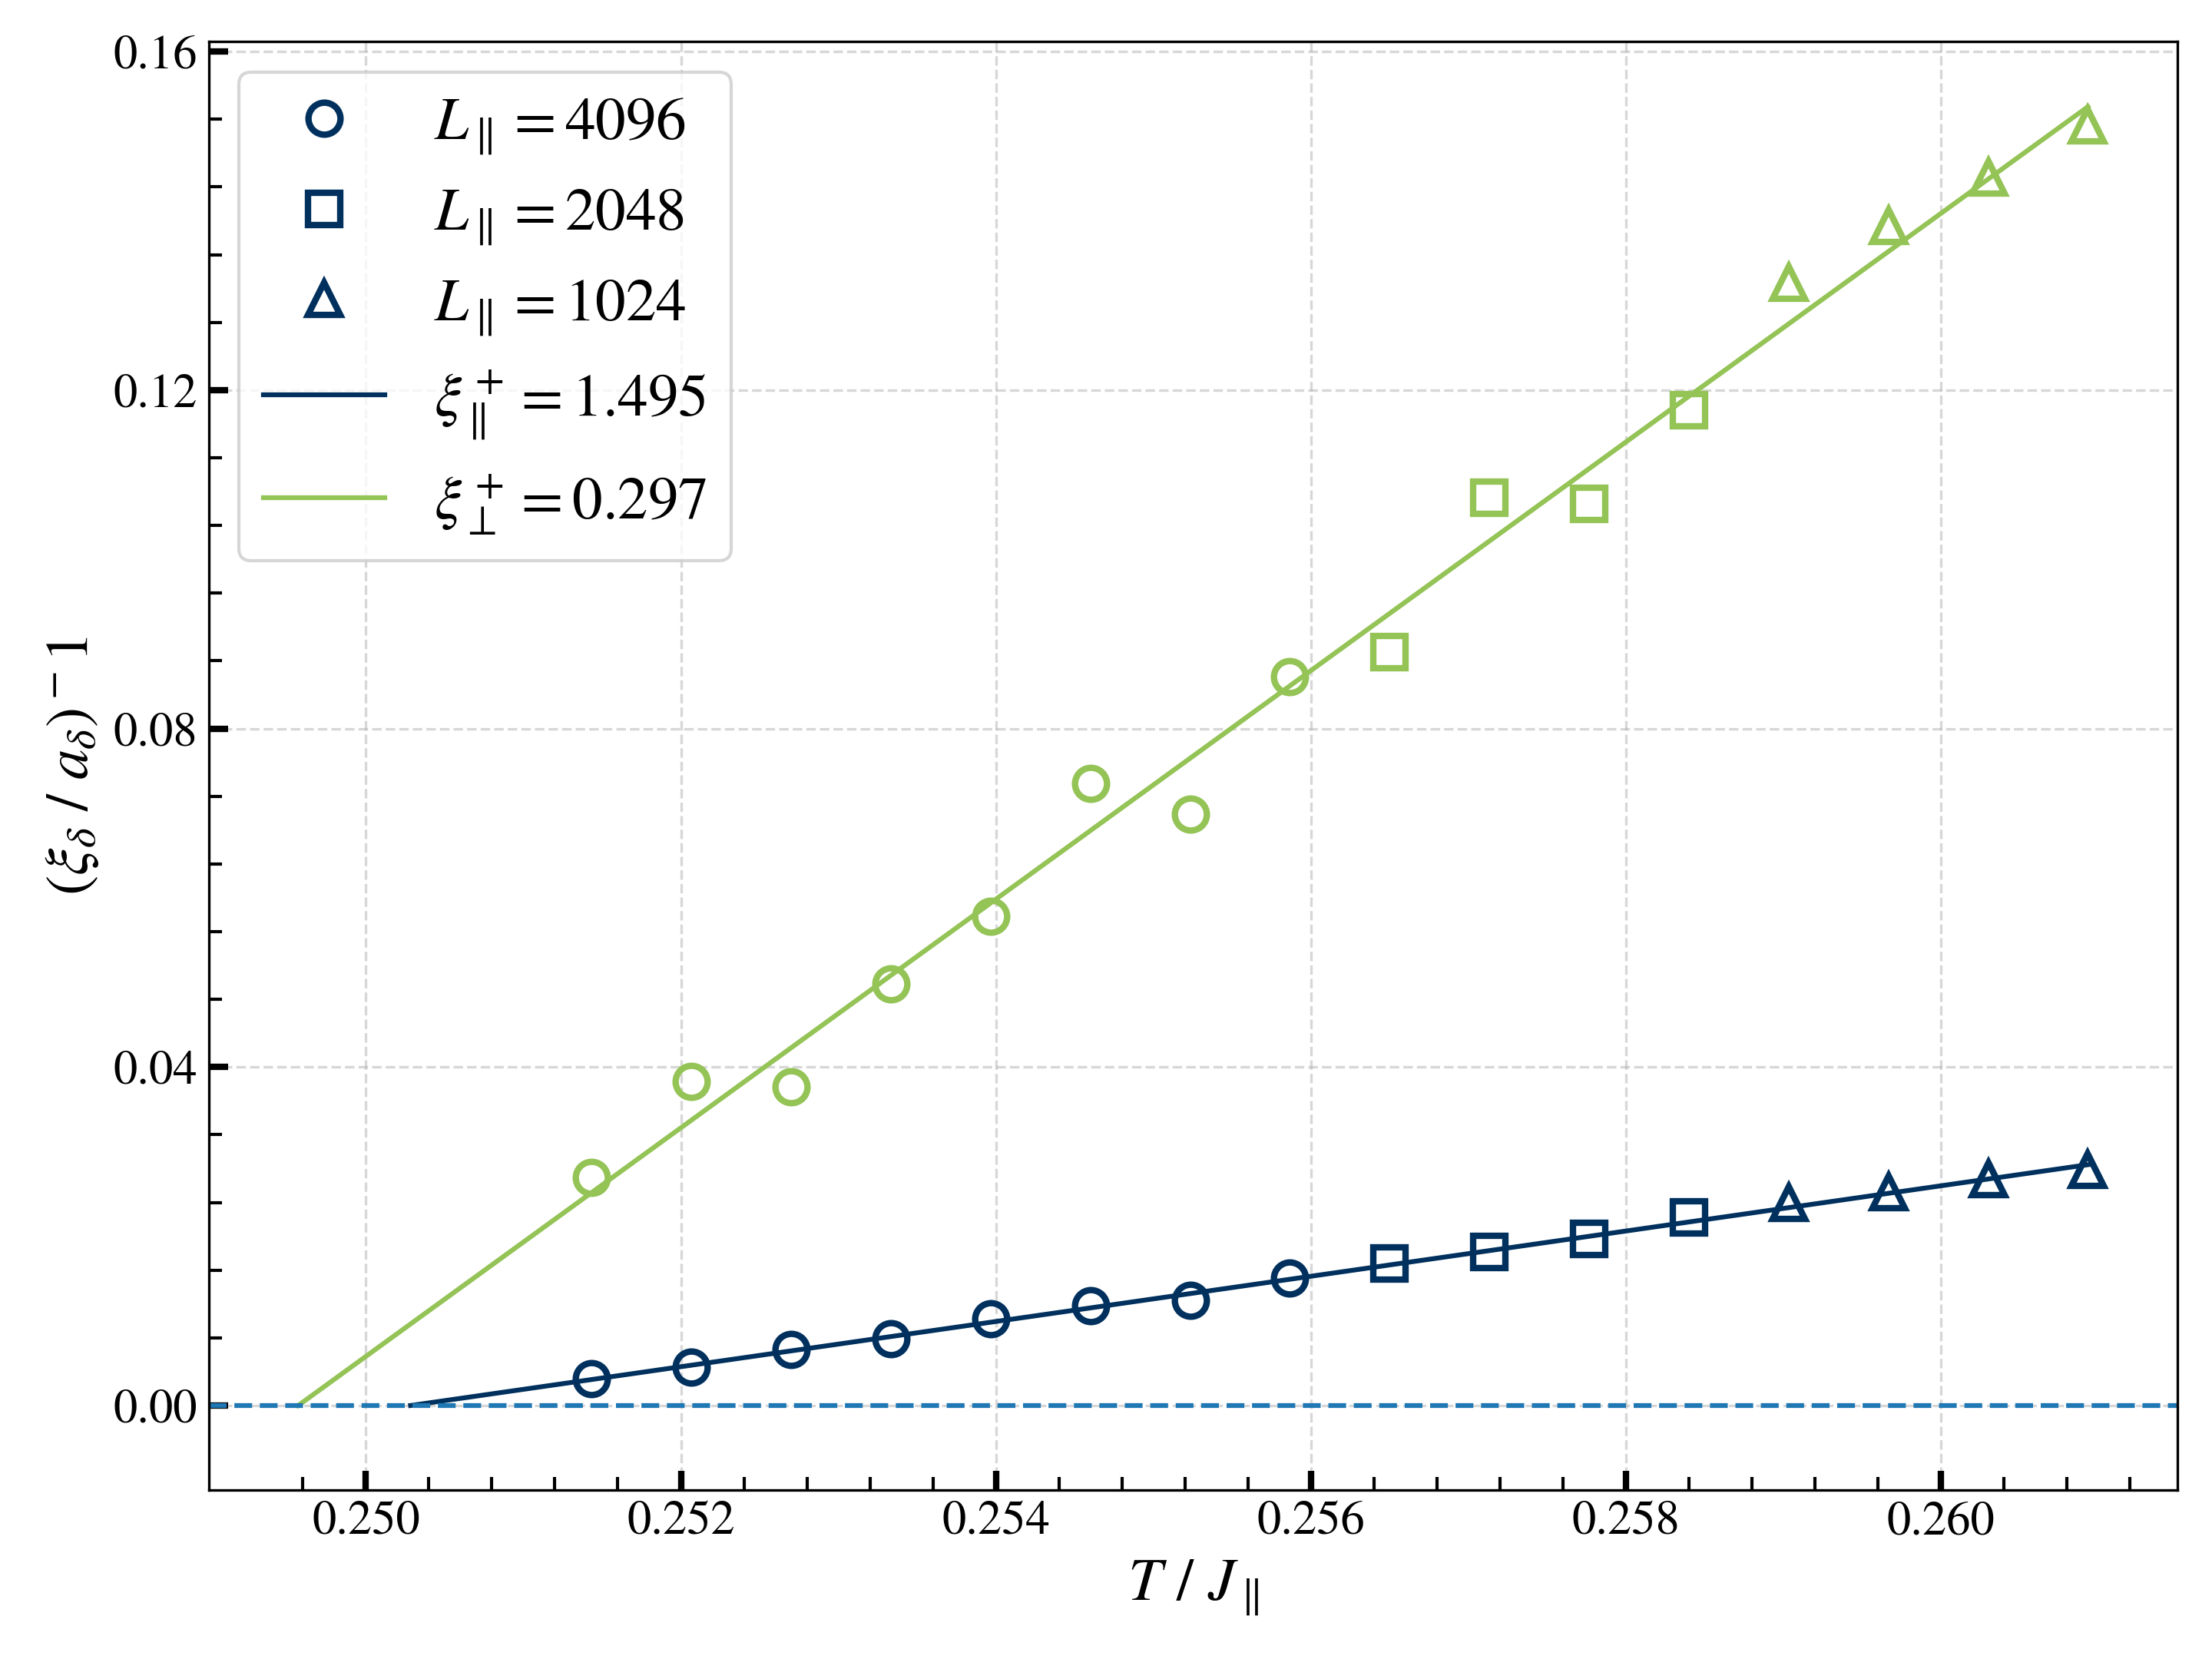
\includegraphics[width=0.95\linewidth]{graphics/xi-inv-divergence-small-h-4.png}
		\end{subfigure}
		\begin{subfigure}{0.475\textwidth}
			\centering
			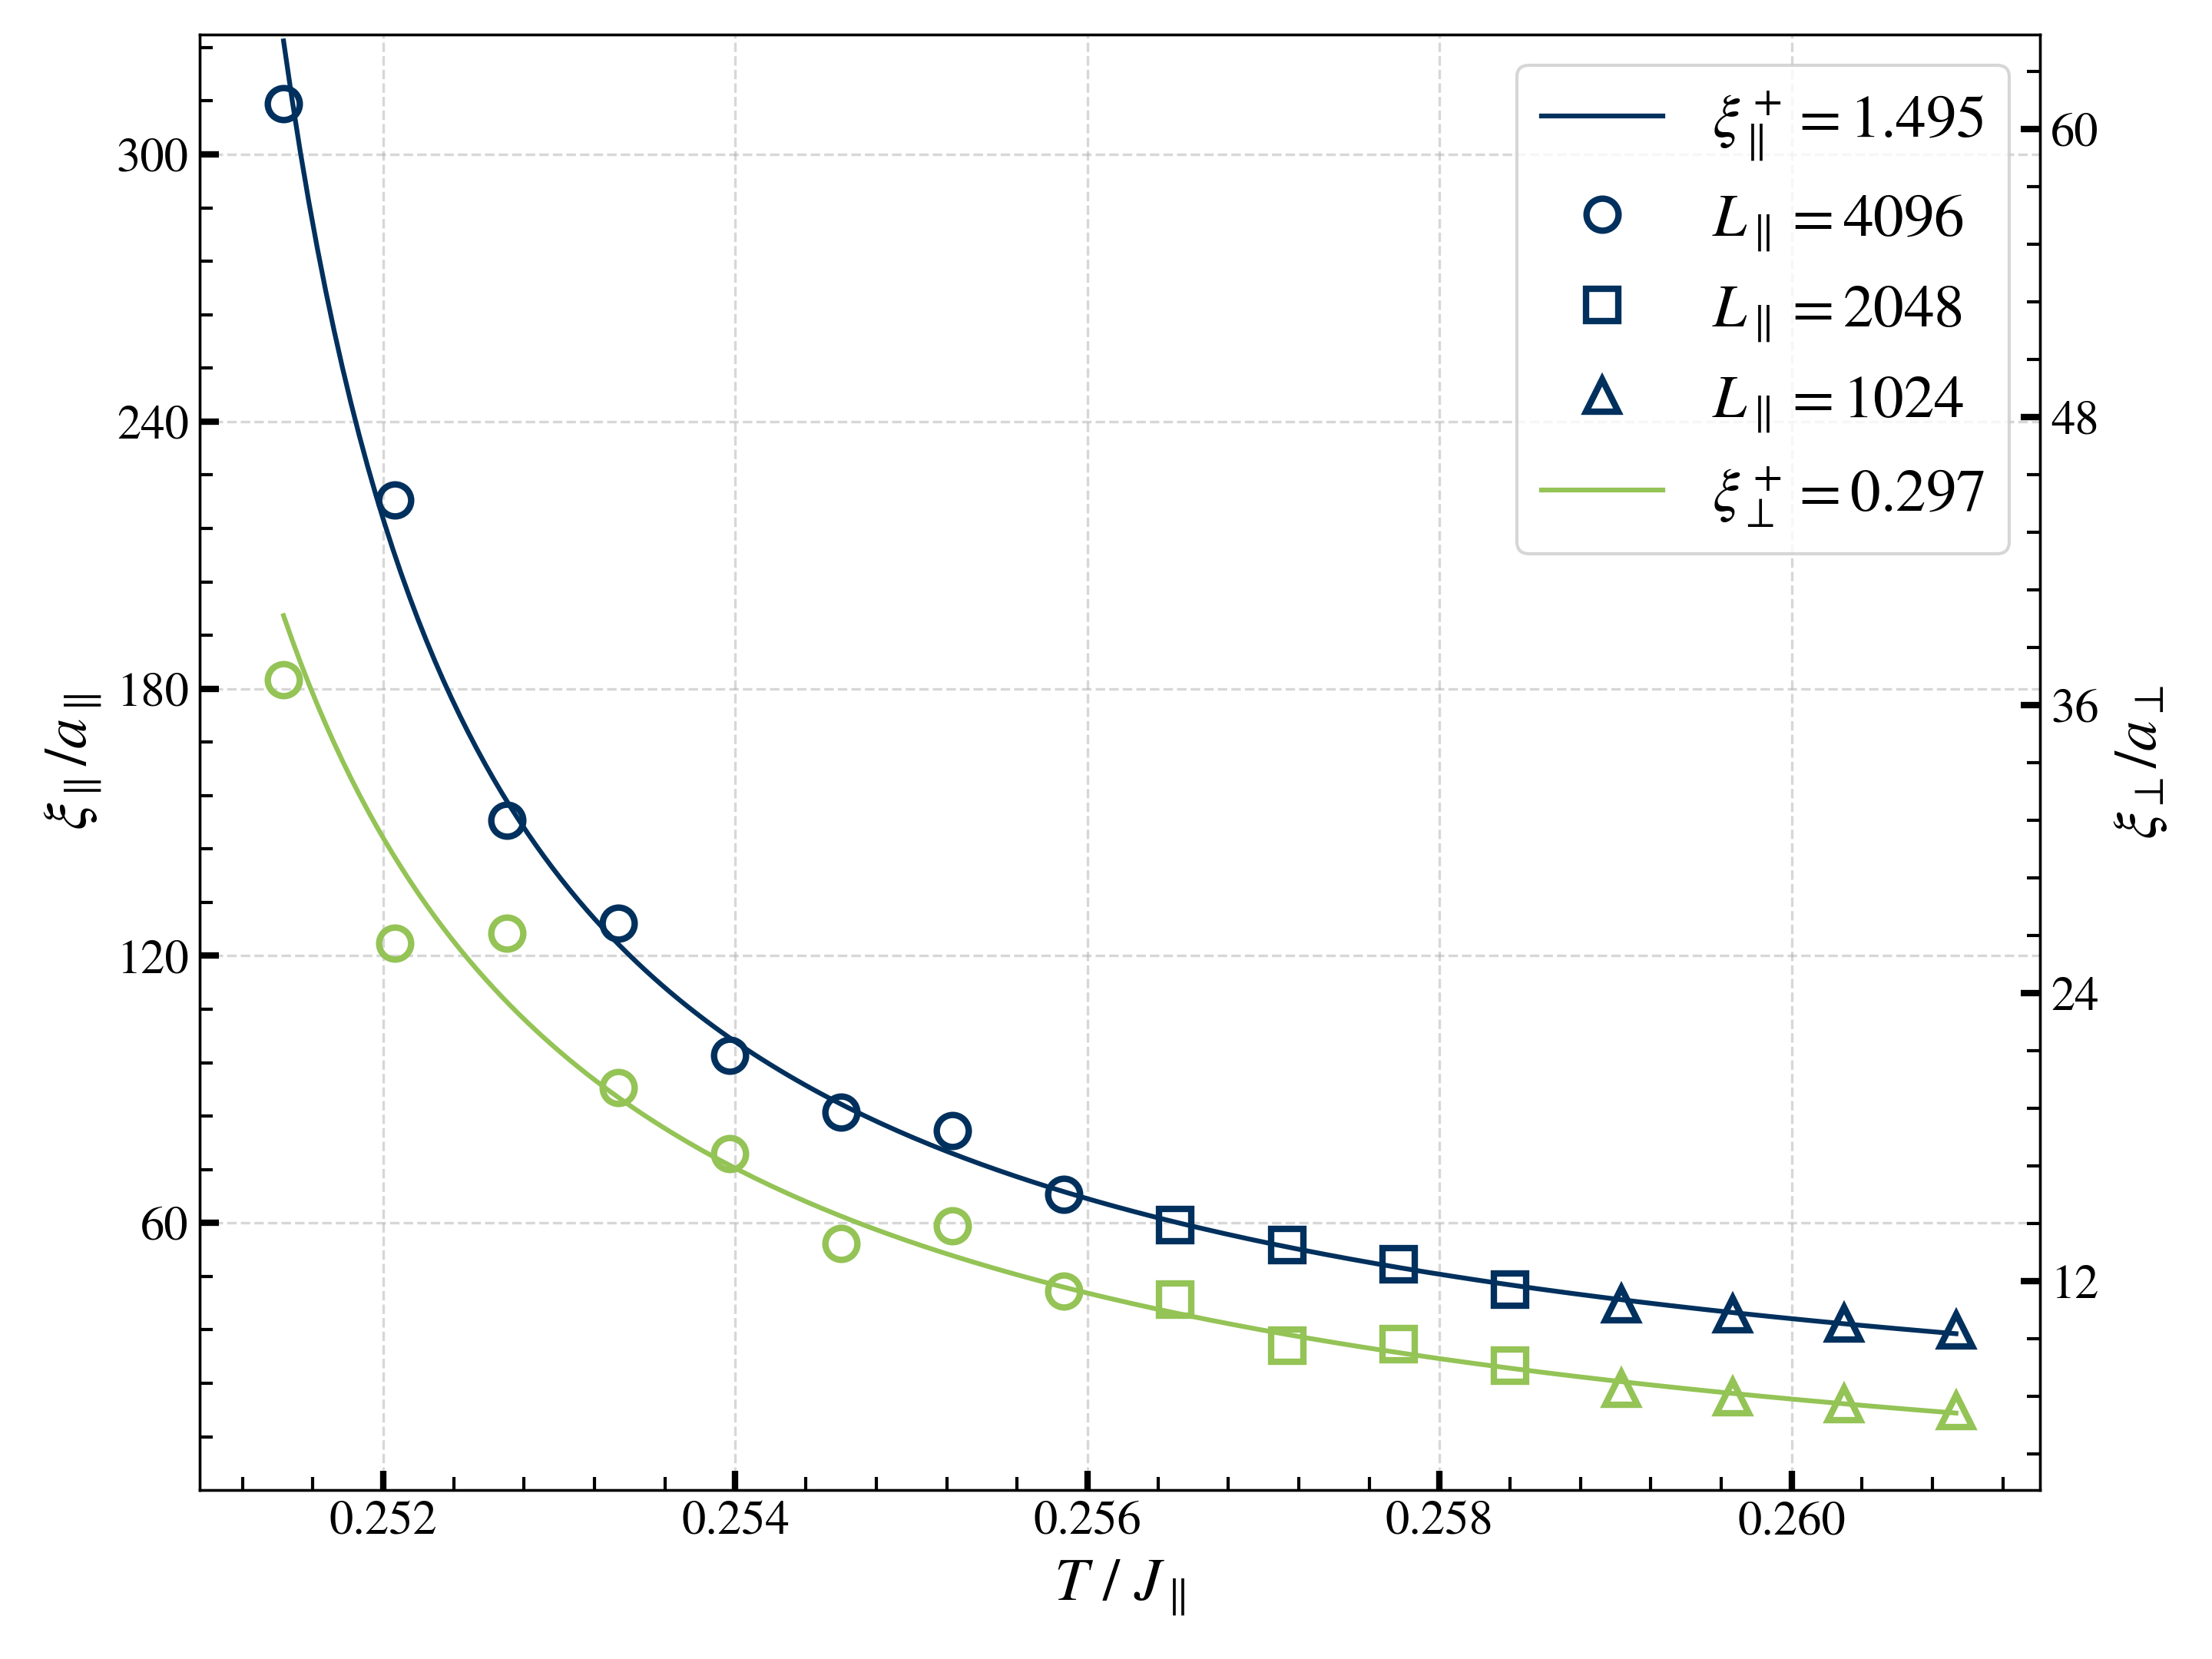
\includegraphics[width=0.95\linewidth]{graphics/xi-divergence-small-h-4.png}
		\end{subfigure} \\ \par\bigskip
		\caption{The correlation length is measured for $T \gtrsim T_c$. \textbf{(a) - (c)}  show the inverse correlation length $(\xi_\delta /	a_\delta)^{-1}$. The system size increases from $L_\parallel =	1024$ to $L_\parallel =	4096$ as the critical point is approached. Linear fits with $\xi_\delta^+$ as in Eq. \eqref{Eq::inv-divergence-fit} are shown for both lattice directions. The systems undergo the phase transition roughly where the lines intersect the zero axis. The ratio of $ J_\parallel /	J_\perp$ in (a) is $30$, leading to an amplitude ratio of $\xi_{\parallel}^+ /	\xi_\perp^+  \approx  5.1$ which is significantly smaller than the Ising value of \eqref{Eq::Ising-Ampl-ratio-xi}, which would be $10.3$. The interaction strength ratio is increased to $ J_\parallel /	J_\perp =	100$ with $h /	T_c =	0.25$ in (b), resulting in  $\xi_{\parallel}^+ /	\xi_\perp^+  \approx  8.9$. This is still smaller than the experimental value but satisfactory for now. Plot (c) has the same parameters as (a), but with a smaller $h / T_c  \approx 0.1$ than in (a) ($h /	T_c \approx 0.5$). With a small symmetry breaking field the absolute value of $\xi_\delta^+$ increase, but their ratio stays essentially the same. In \textbf{(d) - (f)}, the divergence of the correlation length is shown together with the fit from the inverse considerations. (Maybe plot in dependence of $\varepsilon$? The problem is that therefore we would have had to determine the critical temperature beforehand for the used systems. \textcolor{red}{recalculate numbers with final measurements, enumeration})}
		\label{Fig::Amplitude-Result}
	\end{figure}	
	\section{Dynamic Scaling}	
	The dynamic universality classes are subgroups of the static universality classes \cite{hohenberg1977theory} and the adapted anisotropic XY model could be in a different dynamic universality class than the two dimensional Ising model. In the following quench dynamics will be investigated and the dynamic critical exponent $z$ extracted. \\
	
	The dynamics will be studied for the system of \autoref{Fig::Amplitude-Result} (c) and (d), so for a system with 
	\begin{equation}
		J_\parallel /	J_\perp = 100 \qquad \text{and} \qquad \beta_c h \approx	0.5~.
	\end{equation}
	\autoref{Fig::Amplitude-Result} (c) shows that the critical temperature at these parameters is approximately at
	\begin{equation}
		T_c /	J_\parallel \approx 0.1975 \pm ?~.
	\end{equation}
	The used dimensionless parameters are conveniently
	\begin{equation}
		j_\parallel =	10, \qquad j_\perp = 0.1 \qquad \text{and} \qquad \rho =	1.
	\end{equation}
	If large $h$ would have been feasible to simulate, the determined ratio of $J_\parallel / J_\perp $ could have been used together with the phase diagram and the experimental value of $h$ to determine quantitative values for the coupling constants $J_\delta$ of an XY model fitted to the silicon surface. This approach was not successful, but the qualitative and universal results of the dynamic should still be valid. 
	\subsection{The Kibble-Zurek Mechanism}
	First, Eq.~\eqref{Eq::KZM-scaling} and the Kibble-Zurek mechanism will be investigated. Since $\nu$ is already known, fitting the exponent $\nu /	(1 + \nu z)$ to quenched correlation lengths determines $z$. \\
	
	The used quench protocol, i.e the manner in which the system is cooled down, is a isotropic, linear quench following Eq.~\eqref{Eq::Linear-Quench}. The starting temperature $\varepsilon(t_{start}) < \varepsilon(\hat{t})$ is chosen to be sufficiently far away to observe adiabatic system evolution before crossing the freeze-out point. The end temperature $\varepsilon(t_{end})$ is chosen in symmetric distance from the transition point $|\varepsilon(t_{start})|=|\varepsilon(t_{end})|$. Before the quench, the system is randomly initialized and equilibrated with a bath of the starting temperature. \autoref{Fig::quench-process-concept} shows the concept of the quenching process. Colormeshs are constructed to illustrate the dimer buckling angle and connected domains. A checkerboard transformation is applied to the lattice values in order to visualize connected domains.  \\
	
	\begin{figure}
		\centering
		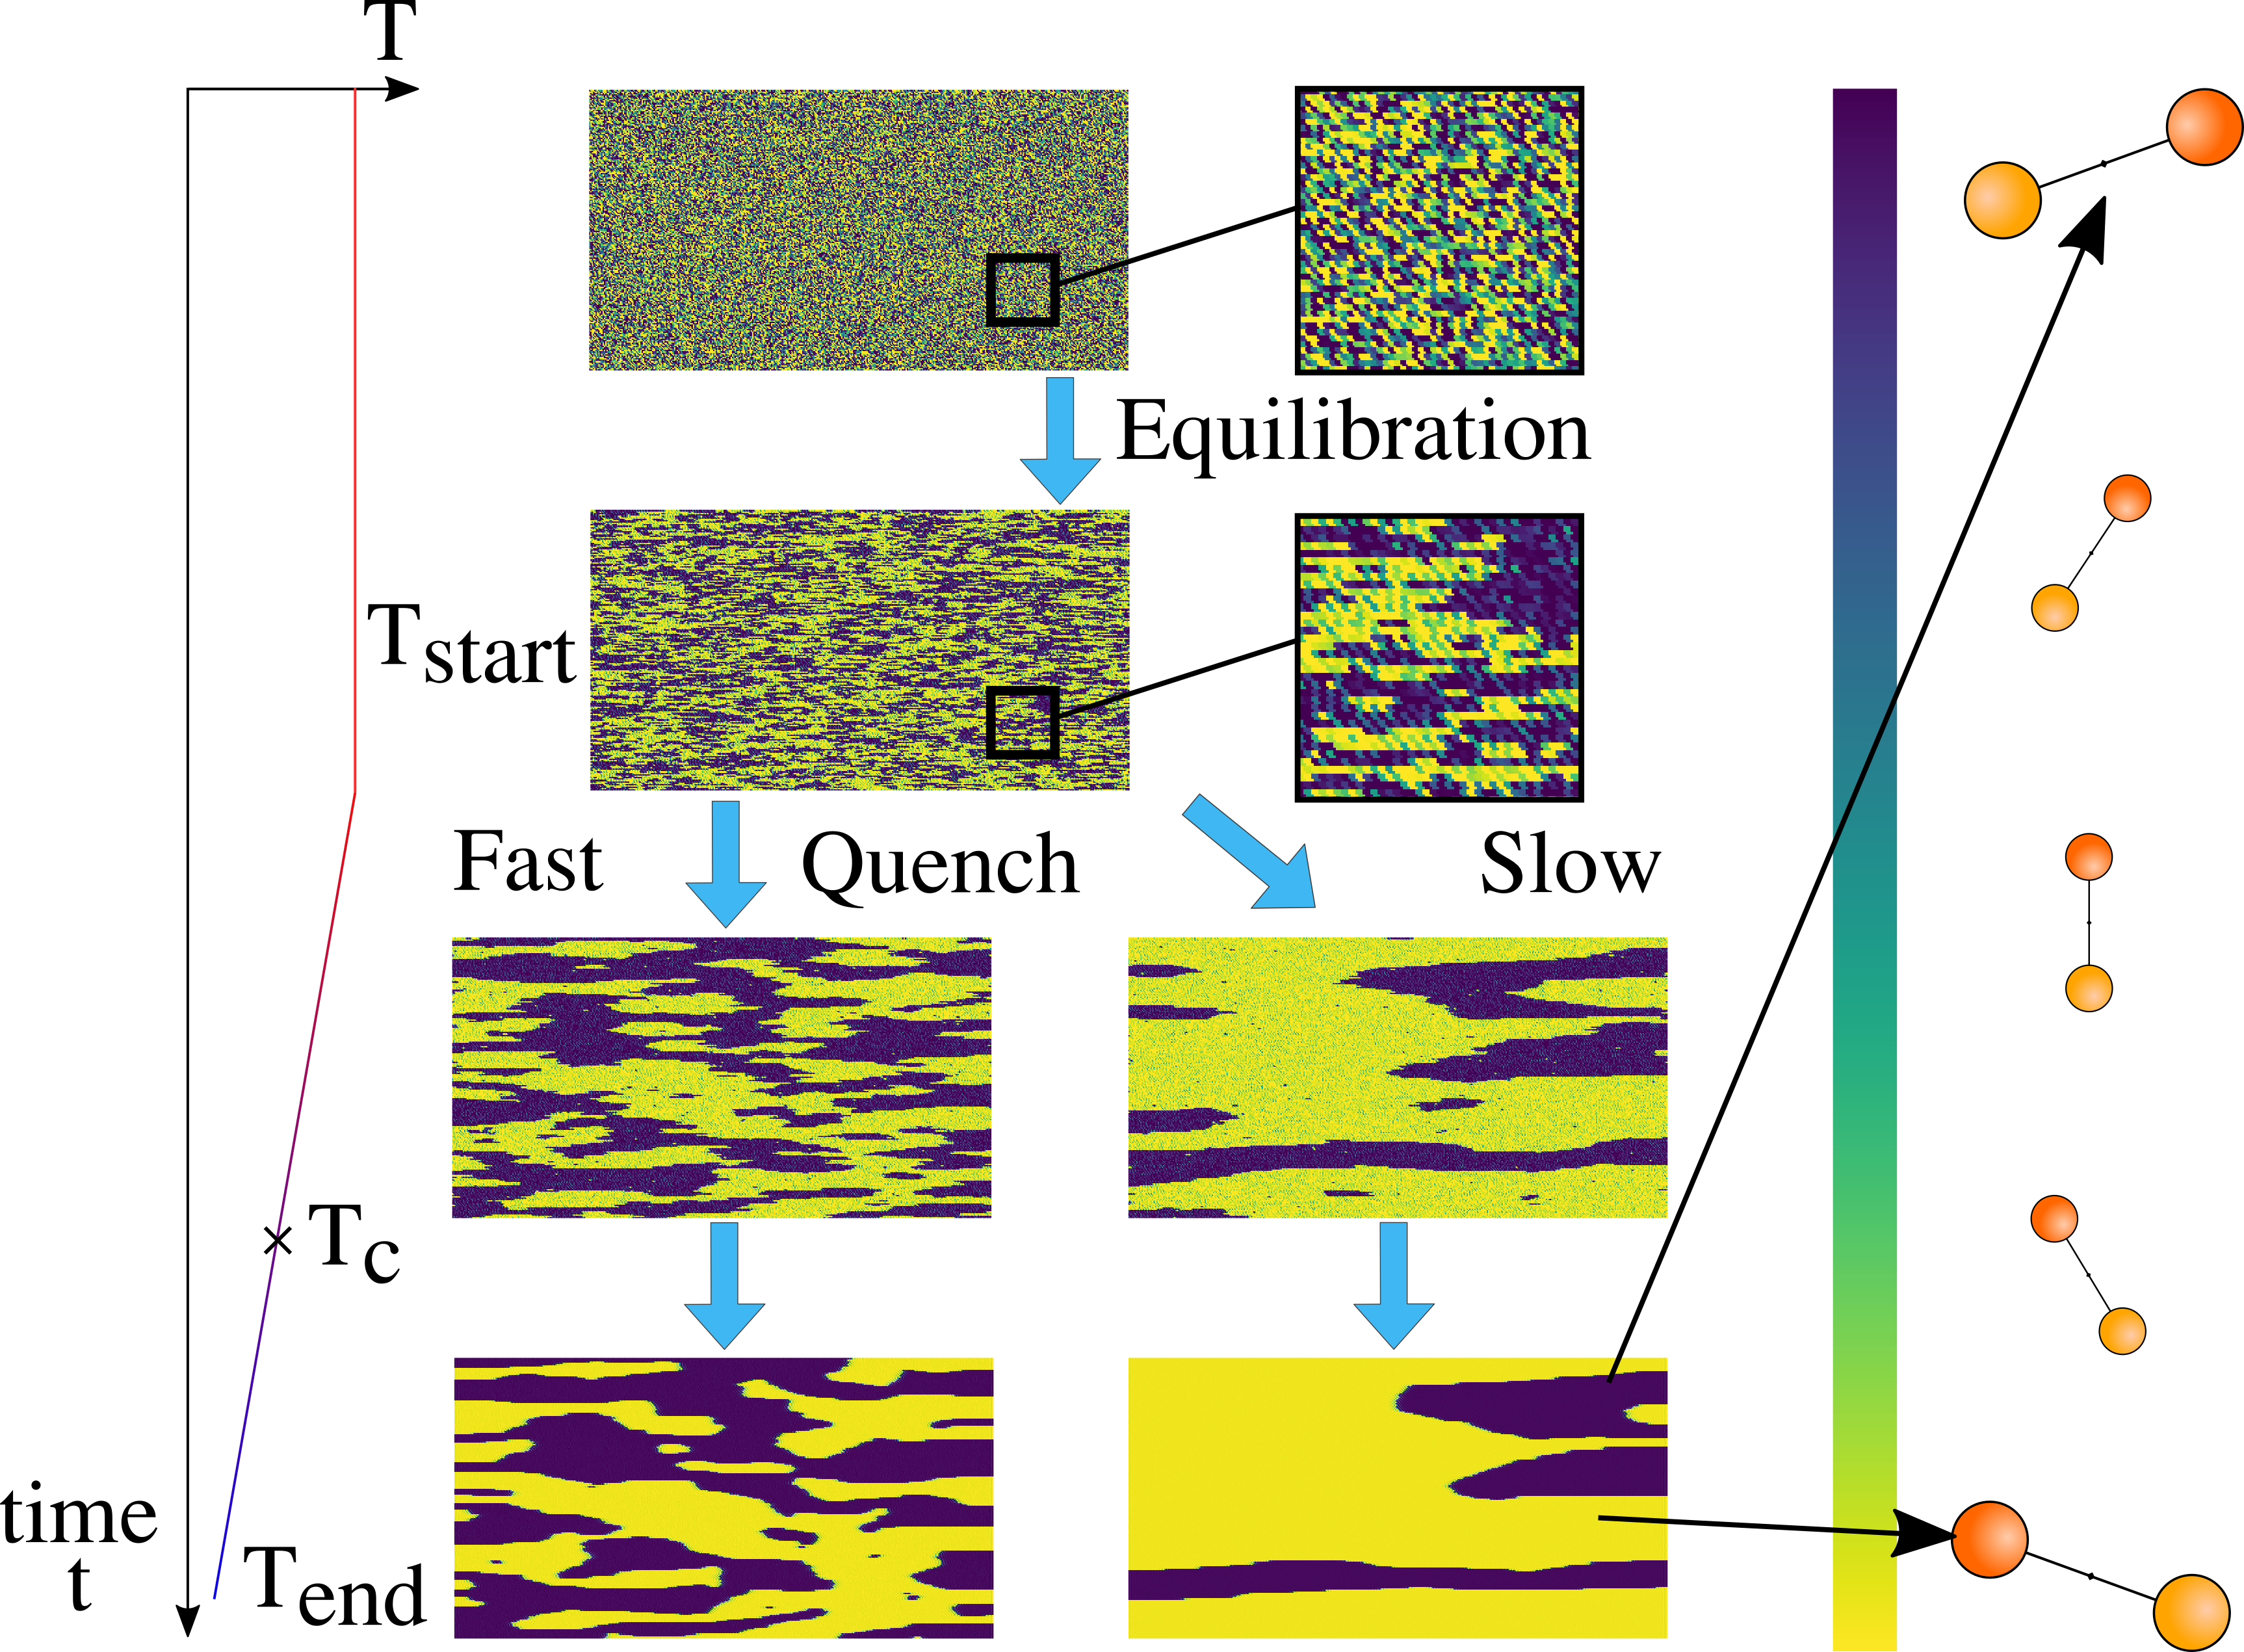
\includegraphics[width=\textwidth]{graphics/Quench-concept-plot.png}
		\caption{Colormeshs of the simulations are shown. The coloring of the squares maps into  the dimer buckling angle. The color bar on the right assigns the color to the dimer position. The temperature diagram on the left shows the temperature $T(t)$ of the reservoir that is coupled to the surface. The quench process is as follows: first, a totally unordered system on the top is coupled to a reservoir with the starting temperature $T_{\text{start}}$. The equilibration phase yields the system below. In the zoom windows show a visual difference in order. After the equilibration the cooling down is started. Depending on how fast or slow the quench is done, following the left or right arrow, smaller or larger domains of order establish. The domains of order can already be made out midway during the quench at $T_c$, but eventually manifest on the way to $T_{\text{end}}$. Note that a checkerboard transformation has been applied to visualize connected domains.}
		\label{Fig::quench-process-concept}
	\end{figure}
	\autoref{Fig::Quench-Result} (a) and (b) shows the current system correlation length in dependence of the quench time. A fit of the frozen correlation lengths $\hat{\xi}$ to \eqref{Eq::KZM-scaling} is performed in \autoref{Fig::Quench-Result} (c) and \autoref{Fig::Quench-Result} (d). It was made sure that $\hat{\xi}_\delta \ll L_\delta$ so that the correlation length extraction method of \autoref{Section::Corr-Length-Calculation} is still applicable. Therefore the system size is doubled if $\hat{xi}_\delta$ exceeds $0.1L_\delta$. For very fast quenches the system behaves initially already non-adiabatic and the correlation lengths plateau. The linear scaling starts after a short transition phase. The extracted KZM exponent of $\nu /( 1 + \nu z) \approx 0.45$ is unusually large. Calculating the dynamic critical exponent yields $z = 1.5$. This is significantly smaller than the in \autoref{Figure::Ising-z-values} shown estimation of $z$ from previous research on the Ising model. \\
	
	Except for small deviations for systems where $\hat{\xi}_\delta \lesssim L_\delta$, the scaling region behaves mostly linear in the logarithmic plot. Hence, there is no initial reason to suspect that the scaling region has not been reached yet. Another reason for the deviation could be that the simulated model belongs to a different dynamic universality class than the Ising model. Hence, a KZM independent $z$-extraction method is applied to further investigate the dynamic critical exponent.	
	\begin{figure}
		\begin{subfigure}{0.475\textwidth}
			\centering
			\includesvg[width=0.95\linewidth]{quench-process-parallel}
		\end{subfigure}
		\begin{subfigure}{0.475\textwidth}
			\centering
			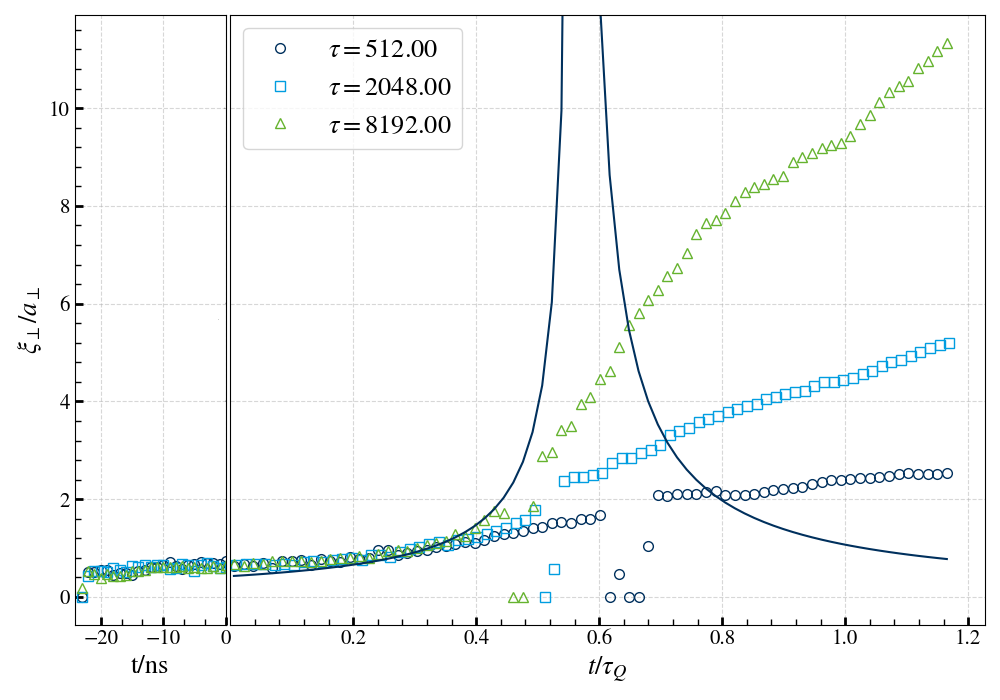
\includegraphics[width=0.95\linewidth]{graphics/quench-process-perp.png}
		\end{subfigure} \\ \par\bigskip
		\begin{subfigure}{0.475\textwidth}
			\centering
			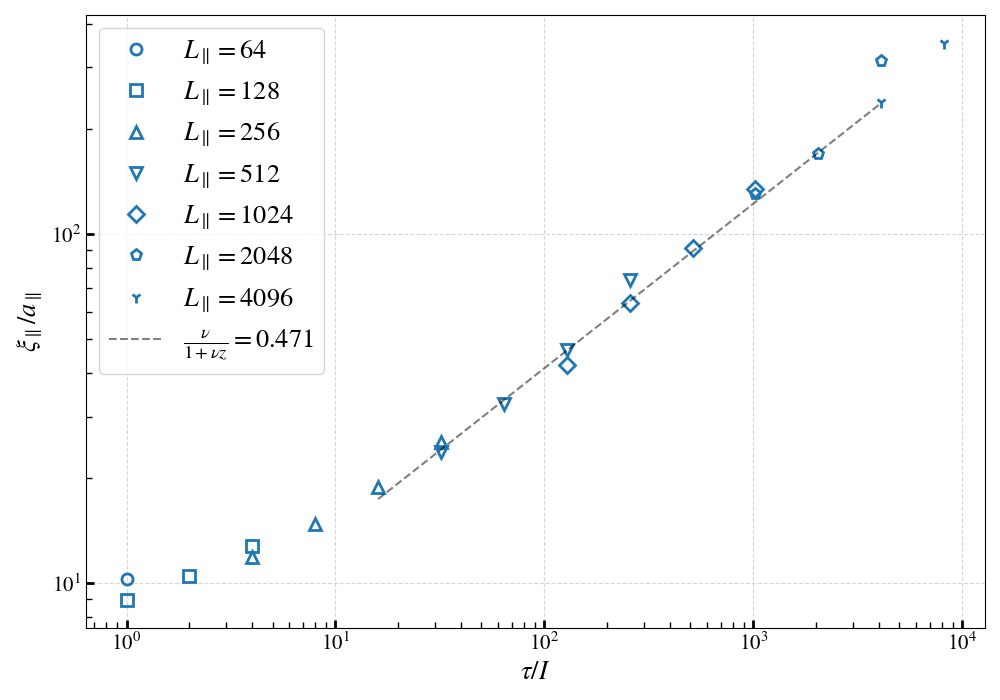
\includegraphics[width=0.95\linewidth]{graphics/tau-xi-parallel3.png}
		\end{subfigure}
		\begin{subfigure}{0.475\textwidth}
			\centering
			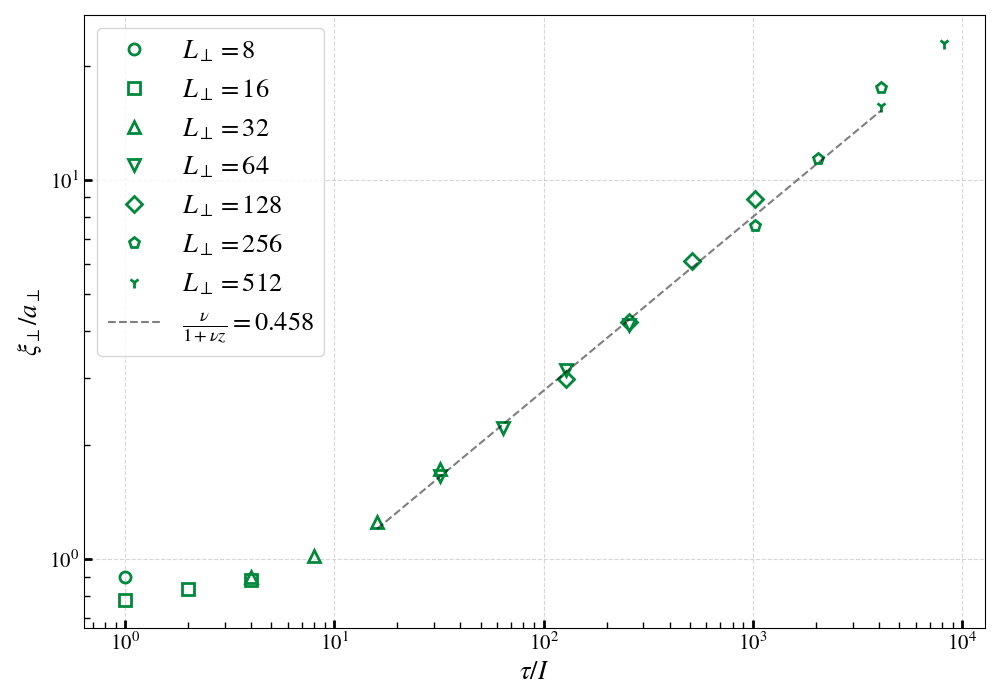
\includegraphics[width=0.95\linewidth]{graphics/tau-xi-perp3.png}
		\end{subfigure}
		\caption{Quenches are examined for the system described at the beginning of \autoref{Section::Dynamic-Scaling}. The system sizes are chosen so that the frozen correlation length is smaller than $L/10$. \textbf{(a)} and \textbf{(b)} show the time resolved quench process, meaning the current system correlation lengths $\xi_\parallel$ and $\xi_\perp$ vs the scaled quench time $t /	\tau_Q$. The left part of the plots shows the equilibration phase. The divergence of the equilibrium correlation length with the amplitude from \autoref{Fig::Amplitude-Result} is also shown. The systems follow the equilibrium correlation length nicely until close to the phase transition. Interesting is that the correlation lengths continue to grow even long after the phase transition is passed. This might be due to a difference between the reservoir temperature and the actual system temperature. Also the inertia of the system which is fully modeled in the langevin dynamics might influence this. \textbf{(c)} and \textbf{(d)} show the KZM scaling, i.e, the frozen correlation length after the quench versus the quench timescale. When the quench is so fast that the system cannot follow the quench even at the start, the frozen correlation length is the equilibrium correlation length of the starting temperature and no scaling is observed. Hence, the scaling is calculated in the linear area. The extracted quench exponent of $\nu / (1 + \nu z) \approx 0.42$ is larger than expected for the Ising model. }
		\label{Fig::Quench-Result}
	\end{figure}
	\subsection{The Critical Exponent $\boldsymbol{z}$}
	One way to examine the dynamic critical exponent is to consider the relaxation of the Binder cumulant including finite size scaling. This method was introduced by Li et. al \cite{li1995dynamic} and will be used in the following to extract $z$. \\
	
	The basis is the time-resolved finite size scaling of the $(n)-$th moment of the magnetization \cite{li1995dynamic}
	\begin{equation} \label{Eq::Dynamic-FSS-M}
		M^{(n)}(t, \varepsilon, L_1) = b^{-n \beta / \nu} M^{(n)}(b^{-z}t, b^{1 /	\nu} \tau, b^{-1} L_1) ~,
	\end{equation}
	with $b =	\tfrac{L_1}{L_2}$ being the spatial rescaling factor of two systems with dimension $L_1$ and $L_2$. Note that the subscript of Eq. \eqref{Eq::lattice-average} has been moved into the parenthesis. Janssen et. al \cite{janssen1989new} determined that the initial correlation length must be very short for Eq. \eqref{Eq::Dynamic-FSS-M} to be valid. Therefore the investigated systems will be prepared in a high temperature, low order state.
	Following the definition of the Binder cumulant in Eq.~\eqref{Eq::Def-Binder-Cum}, one can relate the Binder cumulant of systems of different sizes at the critical point $\varepsilon =	0$ by
	\begin{equation}
		U(t, 0, L_1) =	U(b^{-z} t, 0, L_2)~.´
	\end{equation}
	The exponent $z$ is obtained by finding a time rescaling factor $b^{-z}$ such that the recorded curves for $U_{L_1}$ and $U_{L_2}$ collapse. Since the sample systems are prepared in a high temperature state where $U_L \approx	3$, a relaxation from this value to the equilibrium $U^*$ is expected.
	\begin{figure}
		\centering
		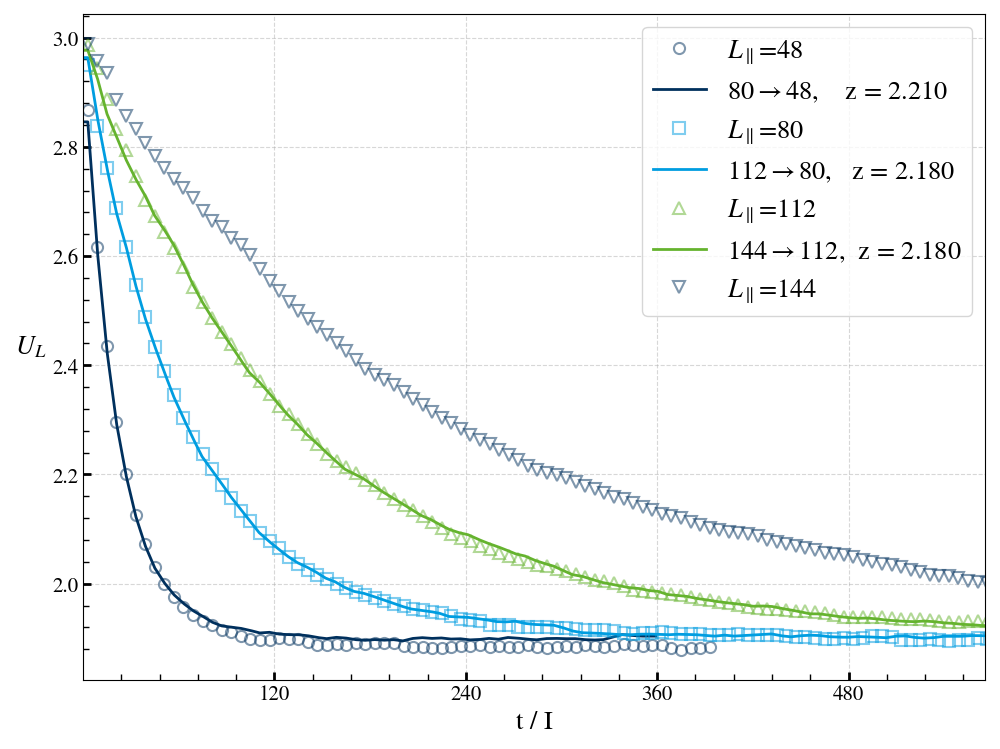
\includegraphics[width=0.925\linewidth]{graphics/z-2.png}
		\caption{The Relaxation of the Binder cumulant is shown versus the dimensionless time for the sizes  $L	\in \{48, 80, 112, 144\}$. The dynamic critical exponent $z$ can be extracted by finding a time rescaling factor $(\frac{L_1}{L_2})^z$ such that $U_{L_1}$ and $U_{L_2}$ collapse.	The best rescaling of $U_{L_1} \rightarrow U_{L_2}$ is selected by rasterizing $z$ in $0.01$ steps and minimizing the squared error between the interpolated curves. The rescalings $144 \rightarrow 112$ and $112 \rightarrow 80$ both yield the dynamic critical exponent $z = 2.18$, which is very close to the Ising universality class $z=2.16$ (see \autoref{Figure::Ising-z-values}). }
		\label{Fig::Cum-Relax-z-extrac}
	\end{figure}
	The results for the rescalings for sizes up to $L_2 =	144$ \autoref{Fig::Cum-Relax-z-extrac}. The cumulants are calculated from 50000 lattices. The rescaling $144 \rightarrow 112$ is more reliable than $112 \rightarrow 80$ since it minimizes the finite size corrections to the scaling law in  \eqref{Eq::Dynamic-FSS-M}. The rescaling $80 \rightarrow 48$ serves as reference and shows strong corrections. Its result $z =	2.18$ is close to the Ising value $z_{\text{Ising}} = 2.16$. The theoretical KZM exponent for $z=2.18$ of $\nu /	(1 + z\nu) = 0.33	$ stands in harsh contradiction to the exponent obtained directly from the quench $\nu /	(1 + z\nu) = 0.45$. Based on the symmetry, it is expected that the adapted anisotropic XY model would show the Ising dynamical exponent. Hence, the deviation might stem from the Kibble-Zurek scaling. Since the system sizes used in the quenches is already very large, strong finite size corrections to the Kibble-Zurek scaling can be ruled out as cause of the deviation. The most sensible explanation for the large Kibble-Zurek scaling exponent is that the cause has to be a systematic difference in the expected Kibble-Zurek mechanics. An idea could be the existence of subleading scalings like reported in \cite{ladewig2020kibble} caused by other scaling fields than the temperature. In our case, $h$ could be such a scaling field. Another cause might be that the KZM scaling regime has not been reached for the fast quenches simulated. \\
	
	If the subleading scalings described in \cite{ladewig2020kibble} are the cause for the found deviation, then the manner in which the phase boundary is crossed influences the KZM	scaling. For a fixed $h$ and starting temperature $T_{\text{start}}$, the system traces a certain path in the phase diagram \autoref{Fig::Phase-Diagram-h} when cooled down. At some point this path crosses the phase boundary at a certain angle, which is in the following called the Quench angle. The angle between the path and the phase boundary is expected to open up scaling regimes, in which the quench exponent does not follow the Kibble-Zurek scaling, but is influenced by other critical exponents. The KZM exponent is obtained by quenching orthogonally to the phase boundary. By varying $h$, the angle of the crossing should change, although it has not been further investigated how much. Also, it has been observed that $h$ has a strong influence on the dynamics. Therefore, in the following we will investigate the effect of $h$ on $z$ as well as on the Kibble-Zurek exponent. Additionally, the damping will be varied as it is expected that it has a significant influence on the dynamics.
	\subsection{Influences on the Dynamics}
	The deviation from the KZM is very curious, especially since it has been validated over the years in numerous theoretical and experimental investigations. Since the KZM exponent is related to universal exponents that do not depend on the microscopic details of the system, it is expected that it does not change if microscopic parameters are varied either. \\
	
	More specifically, the influence of the parameters $h$ and $\eta$ on the dynamics of the system is examined. These two parameters are especially interesting. On the one hand, a distinctive feature of Langevin dynamics simulation is the existence of $\eta$, and, on the other hand, the usage of the experimental $h$ is not possible at the moment so its qualitative influence is all the more important. \\
	
	In addition, som information about the existence of subleading scalings \cite{ladewig2020kibble} might be obtained. Another statement of Ladewig et. al's work \cite{ladewig2020kibble} is that for very long quenches the KZM scaling emerges. This could mean that the in this research performed quenches are to short. \\
	
	The quench results for different $\beta_c h$ are shown in \autoref{Fig::Quench-Result-h} (a) - (d). Besides $\beta_c h$, the parameters are the same as in the last measurement. Comparing the Quenches for large and small $h$ shows that the linear scaling region starts at larger timescales for strong symmetry breaking fields. This is a clear indication that the dynamics of the system slows down with increasing $h$. Apart from that, the symmetry breaking field does not seem to have any influence on the scaling exponent. However, this does not directly disprove the hypotheses that the subleading scalings are the reason for the observed exponent. Further investigations that track the quench angle are needed here. In \autoref{Fig::Quench-Result-h} (e) and (f) the cumulant relaxation method is repeated for small and large $h$. The cumulant takes longer to relax for large $h$. Besides that, the extracted $z$ stays the same and still does not agree with the corresponding quenches.\\
	
	The results for varied $\eta$ are plotted in \autoref{Fig::Quench-Result-eta} (a) - (d). Large dampings shift the linear scaling region to longer quench timescales. Small $\eta$ reveals the existence of a hump in the scaling region. The question arises whether this hump exists for all other measurements and was not observed because of too small quench timescales. For small $\eta$, the quench exponent at the run-off of the hump is $\nu /	(1 + \nu z) =	0.55$. With the current simulation, the hump could not be passed entirely. It is not clear whether the otherwise observed KZM exponent of $\nu /	(1 + \nu z) =	0.45$ arises at larger timescales, or if small dampings increase the quench exponent. The dynamical critical exponent $z$ is extracted in dependence of $\eta$ in \autoref{Fig::Quench-Result-eta} (e) and (f). Large dampings slow down the relaxation of the Binder cumulant. For the small damping, $\eta$ could not be set as small as in the corresponding quench. The finite size corrections seemed to have a stronger influence here. In other words, the exponent $z$ grows with the system size used and it was not feasible to reach a converged value. The rescaling $80 \rightarrow 48$ in \autoref{Fig::Quench-Result-eta} also shows stronger finite size dependence. Apart from that, no indications for the influence of $\eta$ on $z$ are found.\\
	
	The investigations of $\eta$ and $h$ gave some insights on their influences on the dynamics, but the nonuniversal behavior of the KZM	scaling exponent remains unclear for now. Further investigations are needed that determine the influence $h$ and $\eta$ more clearly. In Addition, examinations of the quench angle could be worthwhile.
	\begin{figure}
	\begin{subfigure}{0.475\textwidth}
		\centering		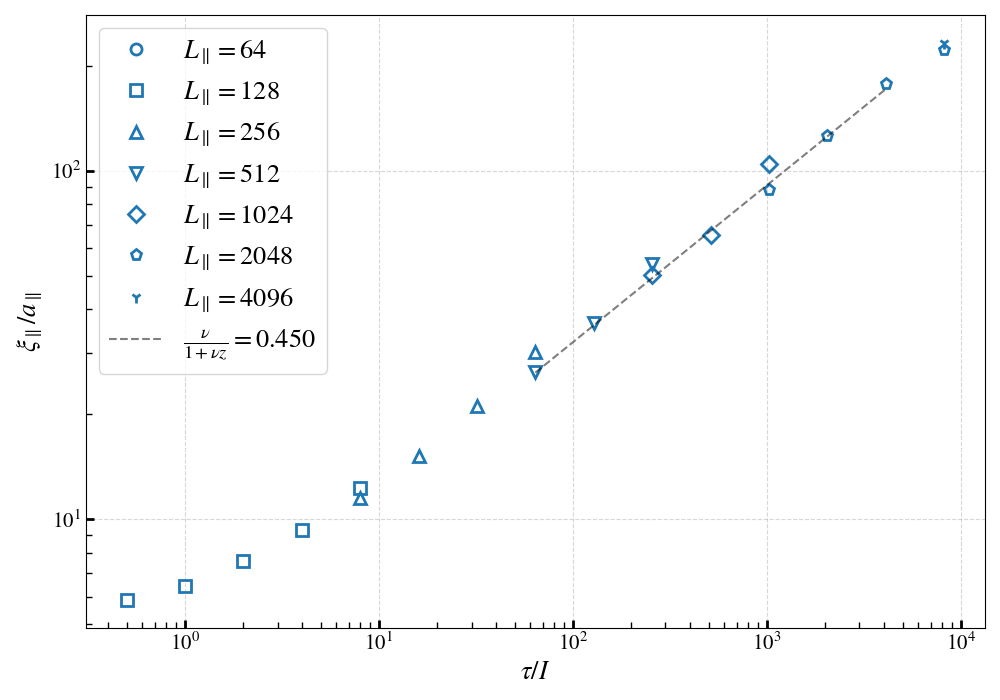
\includegraphics[width=0.95\linewidth]{graphics/tau-xi-parallel-large-h3.png}
	\end{subfigure}
	\begin{subfigure}{0.475\textwidth}
		\centering		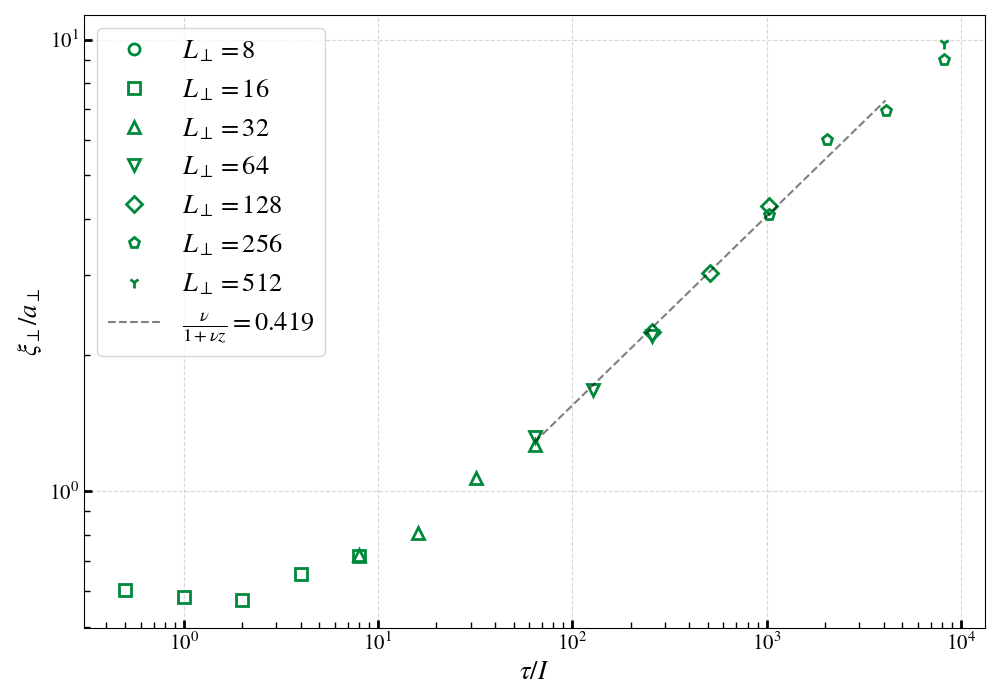
\includegraphics[width=0.96\linewidth]{graphics/tau-xi-perp-large-h3.png}
	\end{subfigure} \\ \par\bigskip
	\begin{subfigure}{0.475\textwidth}
		\centering
		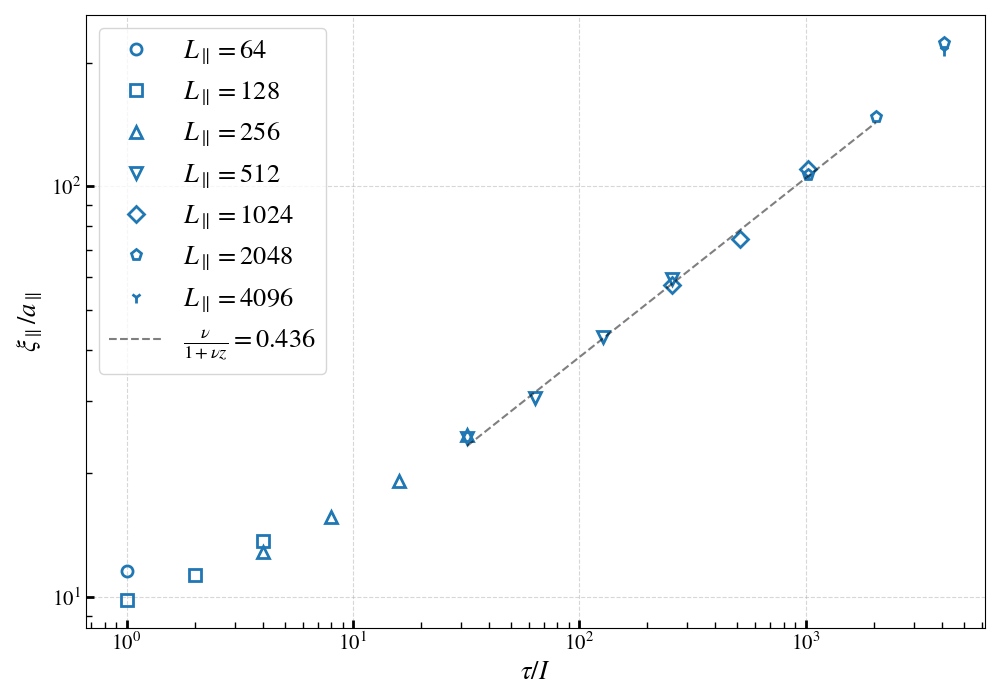
\includegraphics[width=0.96\linewidth]{graphics/tau-xi-parallel-small-h3.png}
	\end{subfigure}
	\begin{subfigure}{0.475\textwidth}
		\centering		
		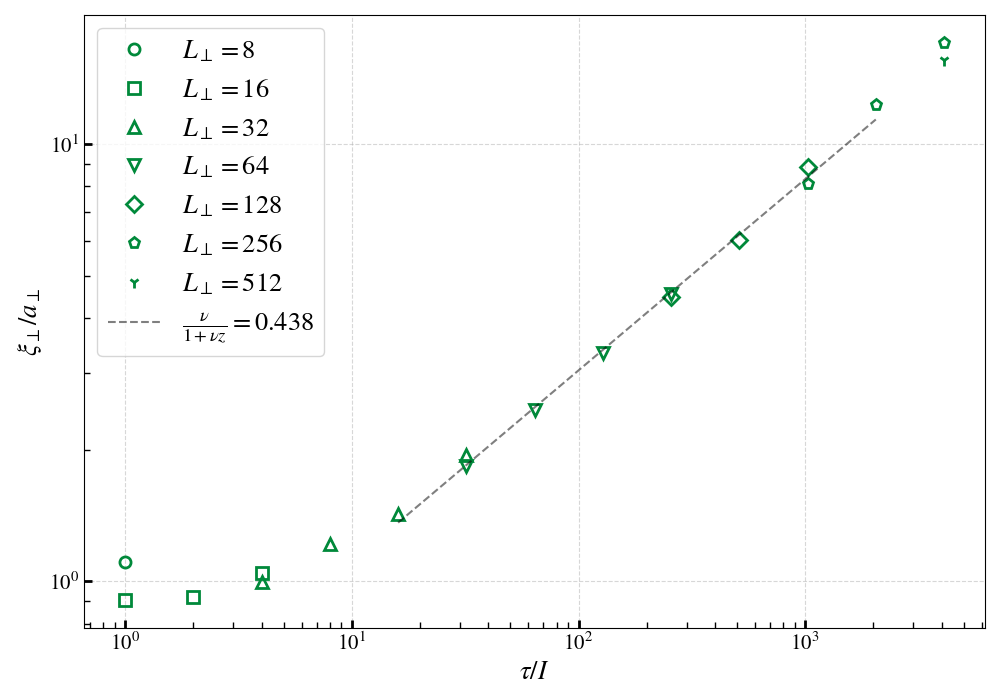
\includegraphics[width=0.96\linewidth]{graphics/tau-xi-perp-small-h3.png}
	\end{subfigure} \\ \par\bigskip
	\begin{subfigure}{0.475\textwidth}
	\centering
	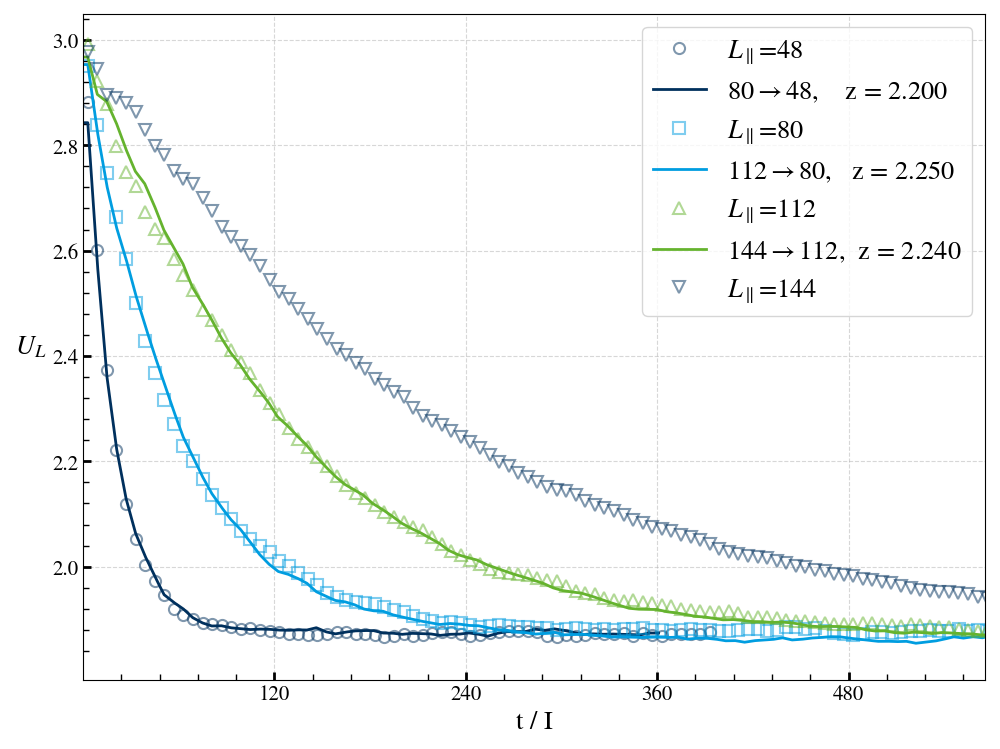
\includegraphics[width=0.96\linewidth]{graphics/z-h-0.5-3.png}
	\end{subfigure}
	\begin{subfigure}{0.475\textwidth}
		\centering		
		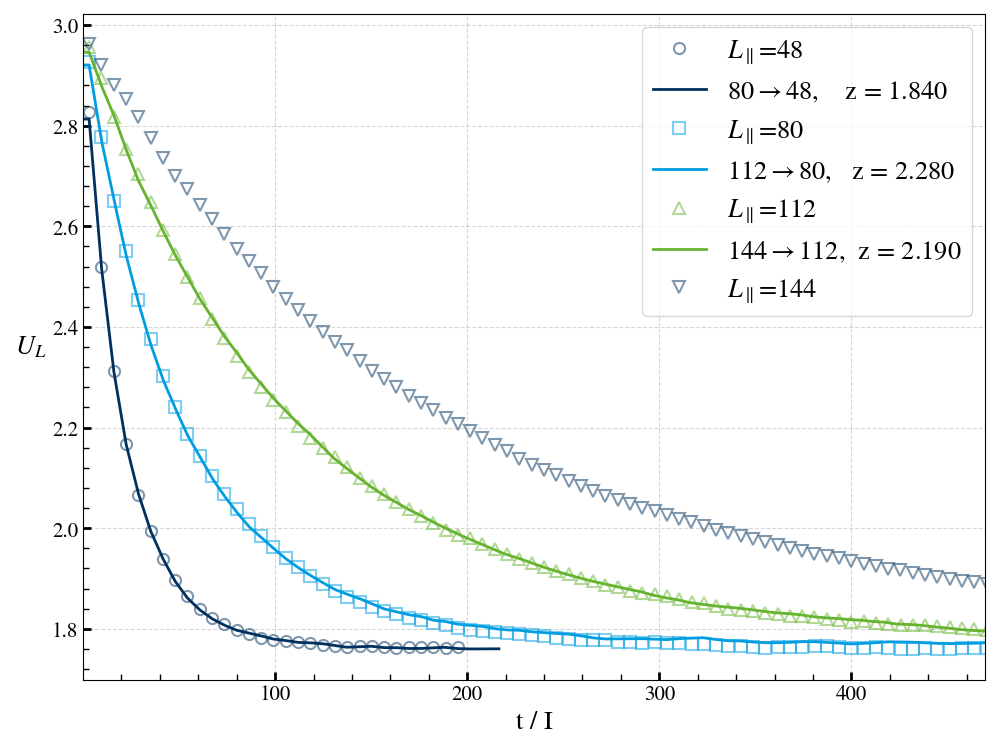
\includegraphics[width=0.96\linewidth]{graphics/z-h-2.png}
	\end{subfigure}
	\caption{Quenches are examined for the different strengths of the symmetry breaking field. \textbf{(a)} and \textbf{(b)} show the results for a large symmetry breaking field of $\beta_c h \approx ?$ for the two lattice directions. 	\textbf{(c)} and \textbf{(d)} represent a small symmetry breaking field of $\beta_c h \approx ?	$.  Like in \autoref{Fig::Amplitude-Result}, stronger symmetry breaking fields reduce the quantitative value of the correlation length. Also as mentioned in \autoref{Section::static-scaling}, the responsiveness of the systems slow down. While the linear scaling for the correlation length across the dimer rows of the large $h$ system starts at about $\tau \approx ?$, it starts for the small $h$ system already at $h = ?$. This has also the effect that we have to quench to far longer times to reach correlation lengths that max out the largest used system size of $L_\parallel = ?$. Besides that, the KZM exponent seems to be independent of the value of $\beta_c h$. Figure \textbf{(e)} and \textbf{(f)} show the relaxation of the Binder cumulant for systems with $\rho = 0.5$ and $\rho = 2$. The large symmetry breaking field slows down the dynamics, but does not have an influence on the dynamic exponent.}
	\label{Fig::Quench-Result-h}
	\end{figure}		
	\begin{figure}
		\begin{subfigure}{0.475\textwidth}
			\centering		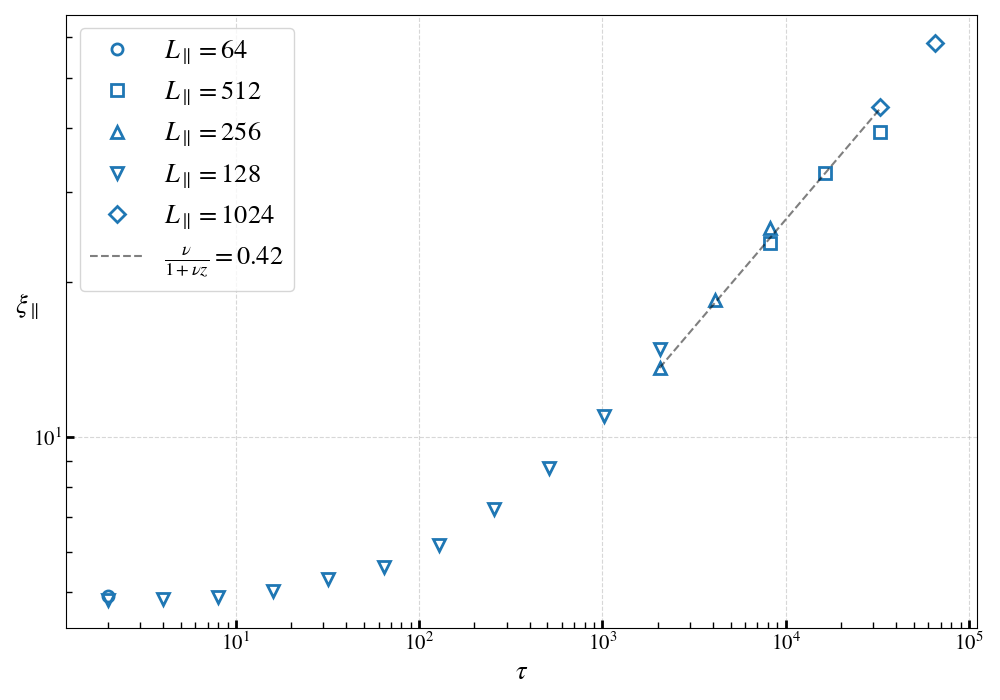
\includegraphics[width=0.97\linewidth]{graphics/tau-xi-parallel-large-eta.png}
		\end{subfigure}
		\begin{subfigure}{0.475\textwidth}
			\centering		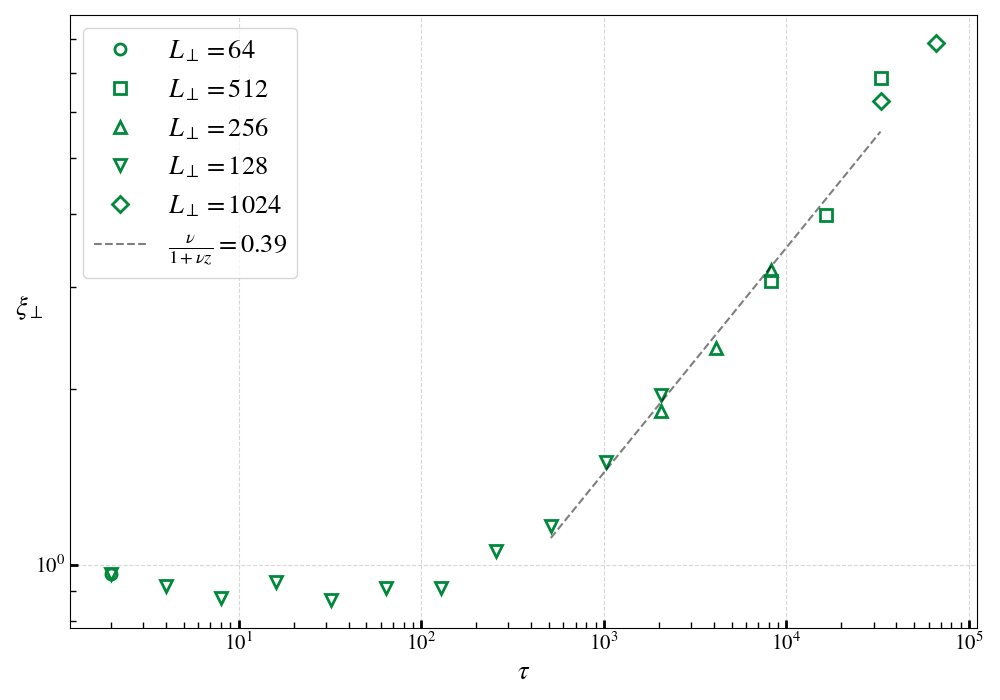
\includegraphics[width=0.97\linewidth]{graphics/tau-xi-perp-large-eta.png}
		\end{subfigure} \\ \par\bigskip
		\begin{subfigure}{0.475\textwidth}
			\centering
			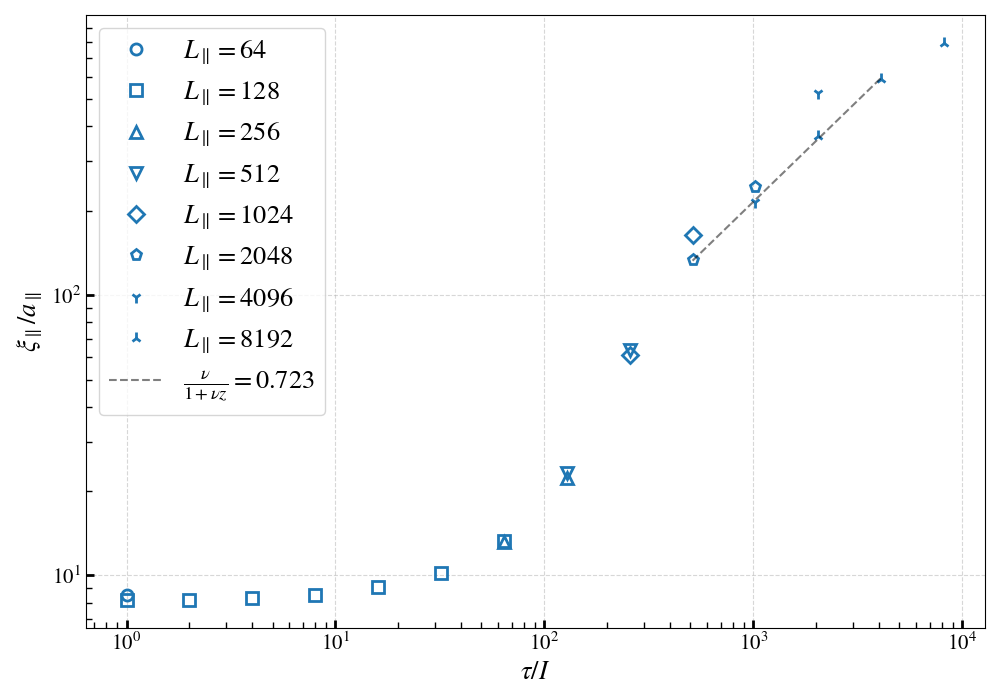
\includegraphics[width=0.97\linewidth]{graphics/tau-xi-parallel-small-eta-2.png}
		\end{subfigure}
		\begin{subfigure}{0.475\textwidth}
			\centering		
			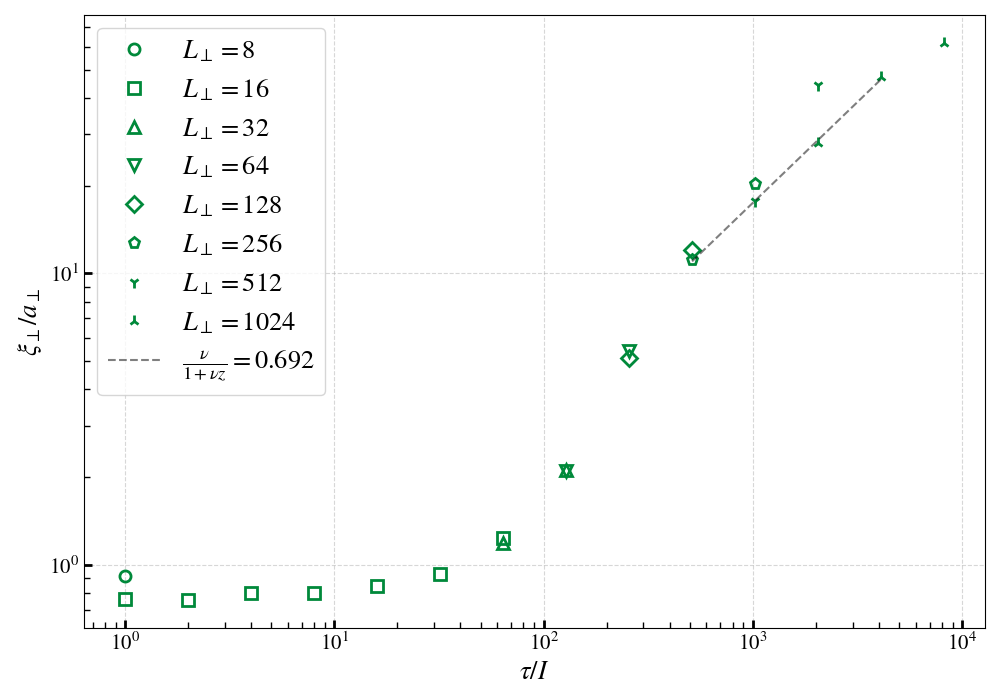
\includegraphics[width=0.97\linewidth]{graphics/tau-xi-perp-small-eta-2.png}
		\end{subfigure} \\ \par\bigskip
		\begin{subfigure}{0.475\textwidth}
			\centering		
			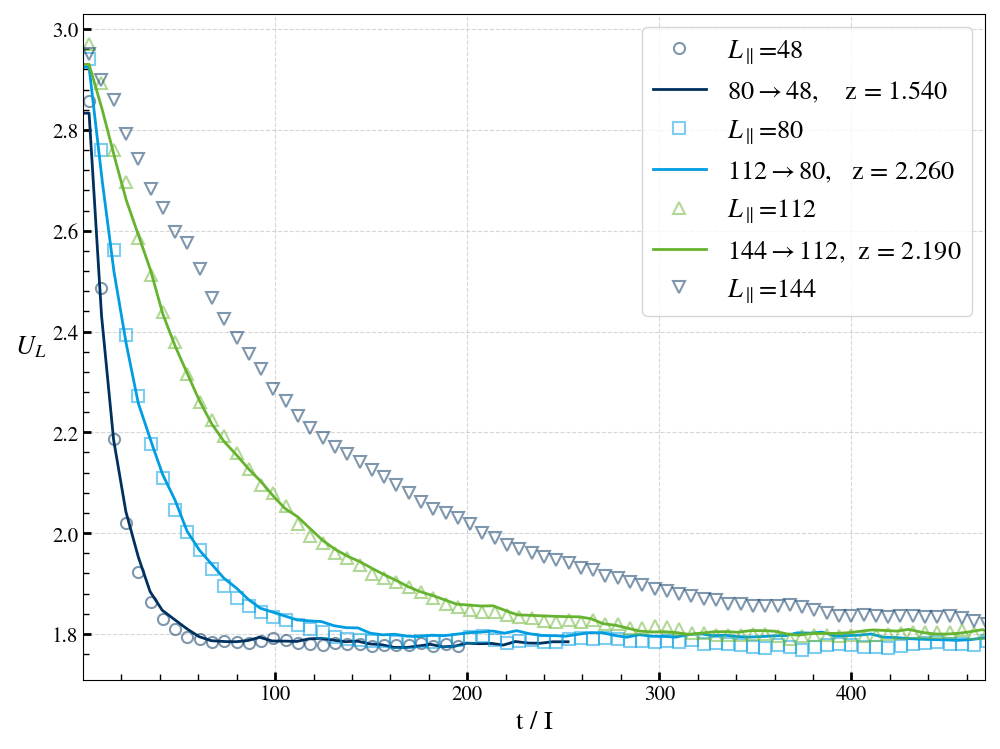
\includegraphics[width=0.97\linewidth]{graphics/z-eta-0.5.png}
		\end{subfigure}
		\begin{subfigure}{0.475\textwidth}
			\centering
			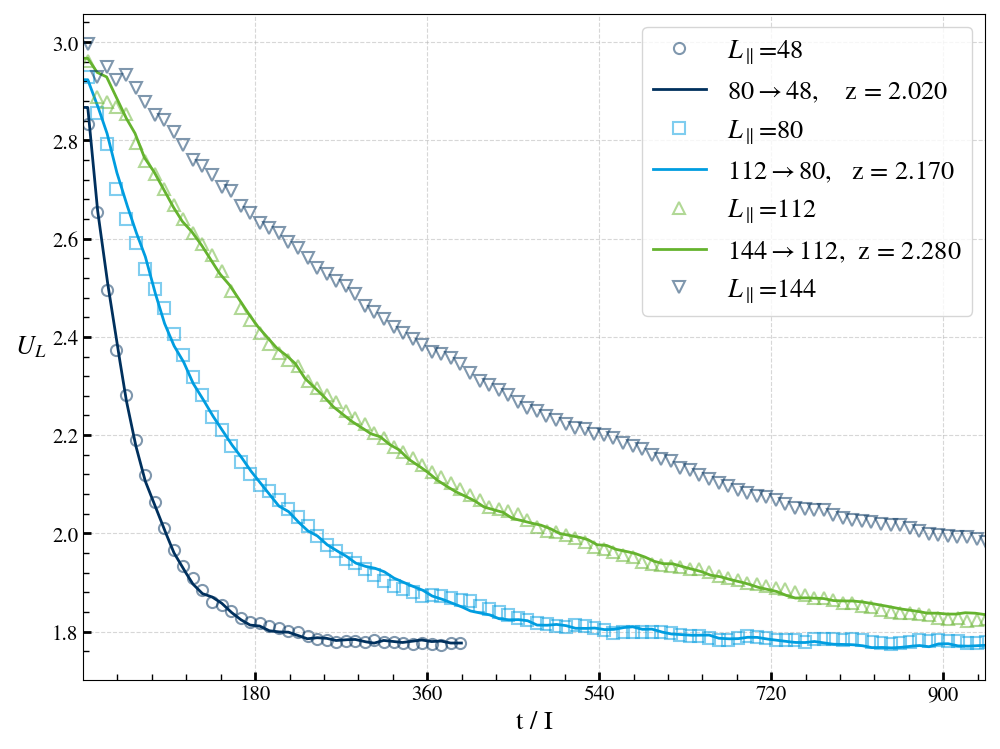
\includegraphics[width=0.97\linewidth]{graphics/z-eta-5-2.png}
		\end{subfigure}
		\caption{Quenches are examined for the different $\eta$. \textbf{(a)} and \textbf{(b)} show the results for a large dampening of $\eta =	?$. 	\textbf{(c)} and \textbf{(d)} are the results for a small damping of $\eta =	?$. Compared to \autoref{Fig::Quench-Result} (c) and (d), the KZM	scaling region starts later for large damping. The KZM exponent seems to be identical though. For small damping, a hump in the scaling becomes visible. This is very interesting and might be related to \cite{ladewig2020kibble}. It gives rise to the question of whether this hump exists for all the other curves as well and has not been reached due to too small timescales. This could be one explanation for the systematically to large KZM exponent that we observe. Figure \textbf{(e)} and \textbf{(f)} show the relaxation of the Binder cumulant for systems with $\eta = 0.5$ and $\eta = 5$. The large damping slows down the dynamics significantly. Small dampings seem to be more strongly influenced by finite size corrections as the rescaling of $80 \rightarrow 48$ indicates.}
		\label{Fig::Quench-Result-eta}
	\end{figure}		
	\section{Discussion}
	The adapted XY model, developed to describe the Si(001) surface, is largely in line with the theory. This includes the phase diagram, the static critical exponent $\nu$, probably the correlation length amplitude ratio $\xi_\delta^+ /	\xi_\delta^-$ and the dynamic critical exponent $z$. Interesting is here that the renormalization group calculations from José et al \cite{jose1977renormalization} that were initially performed for integer $p$, seem to be valid also for rational $p$. Also, cutting the phase space in half by introducing a parameter $m$ in \eqref{Eq::m-introduction} does not seem to have an effect whatsoever. Our assumption is that the universal behavior of the treated model does only depend on the continuity of the state parameter and the number of minima of the symmetry breaking field. José et. al's predictions have previously been studied by Monte Carlo methods \cite{landau1983non, rastelli2004monte} for $p=4$. Both find a second order phase transition with non-universal critical behavior, as is expected for $p=4$. Rastelli et. al \cite{rastelli2004monte} find the Ising critical exponent in the limit of large $h$. The presented investigations join them in confirming José et. al and expand the argument to rational $p$. and the dynamic universality class. \\
	
	The description of the silicon surface using the anisotropic XY model differs from previous Ising model descriptions by the fact that much larger interaction strength ratios of $J_\parallel^{\text{XY}} / J_\perp^{\text{XY}} \approx 100$ are needed to reproduce the experimental correlation length ratio of $\xi_\parallel^+ /	\xi_\perp^- \approx 10$. The theoretical result of the Ising model \eqref{Eq::Ising-Ampl-ratio-xi} yields $J_\parallel^{\text{XY}} / J_\perp^{\text{XY}} \approx 30$. Also, roughly a factor of two larger coupling constants are required to reproduce the experimental transition temperature. This is expected \cite{aizenman1980comparison} since $J \cos \Delta \vartheta < J$.\\

	An advantage of the Langevin dynamics modeling of the silicon surface is that, in principle, the dynamics on the surface can be examined in a more realistic manner. A large disadvantage is though that it is significantly more computationally expensive. The effect of strong symmetry breaking fields proves to slow down the dynamics on the surface drastically. With the current methods neither equilibration nor significant dynamic phenomena are feasible to simulate. The slowdown of the dynamics has been observed in both the quenches and the relaxation of the binder cumulant in \autoref{Fig::Quench-Result-h}. Other than the slowdown, the strength of $h$ does not seem to influence the KZM	scaling. Our simulations predict a final value of
	\begin{equation}
		\frac{\nu}{1 + \nu z} =	0.4,  \text{         shouldnt even be called that way?}
	\end{equation}
	which would constitute a significant divergence from the Ising scaling. The nature of this divergence is not clear at the moment and the explanations could range from simple to fast quenches to something more fundamental. Schaller et al. \cite{schaller2023sequential} used kinetic Monte Carlo methods to simulate an Ising model with the values of Eq. \eqref{Eq::Exp-coupling-ising}. They extract a KZM exponent of $\nu /	(1 + \nu z) =	0.35$, which is in good accordance with the theoretical Ising value. The quench angle in the $\beta J_\parallel-\beta J_\perp-$plane of the phase space is quite similar between the Ising model and the XY model. Hence, the quench angle in this cross section may be ruled out as source of the KZM exponent deviation. However, other than in the antiferromagnetic XY model, the barrier height of the on-site potential has no influence on the critical point in the Ising model. The quench angle in the $h$-dimension of the anisotropic XY model may therefore still be the cause of the abnormally large KZM exponent. \\
	
	Schaller et. al further observe that the frozen correlation length ratio $\hat{\xi}_\parallel / \hat{\xi}_\perp$ in the linear scaling region is twice the equilibrium ratio $\xi_\parallel / \xi_\perp$. They explain this phenomenon with the argument that the weakly coupled direction diverges earlier from the equilibrium behavior than the strongly coupled direction. This is also observed in the fact that the linear KZM scaling regime starts later for the weakly coupled direction, which is clearly also observed for in this investigations. The effect is strongest for the strong symmetry breaking field in \autoref{Fig::Quench-Result-h}. In the anisotropic XY model the ratio $\hat{\xi}_\parallel / \hat{\xi}_\perp$ depends strongly on $h$. We find the values
	\begin{table}[h]
	\centering
	\begin{tabular}{c | c c c}
		$\beta_c h$  & $\quad$ 0.3 $\quad$ & 0.5 $\quad$ & 1.8\\
		\midrule
		$ \left({\hat{\xi}_\parallel}/{\hat{\xi}_\perp}\right) \Big / \Big({{\xi}_\parallel} /	{{\xi}_\perp}\Big) $ & 1.3 & 1.5 $\quad$ & 2.0 \\
		\end{tabular}
		\label{Table::frozen-corr-length-ratio}
	\end{table}
	\textcolor{red}{Oder lieber einfach im Text?} We find that the ratio $ \left({\hat{\xi}_\parallel}/{\hat{\xi}_\perp}\right) \Big / \Big({{\xi}_\parallel} / {{\xi}_\perp}\Big) $ increases from about $1.3$ at $\beta_c h \approx	0.3$ to $1.5$ at $\beta_c h \approx	0.5$ and finally to $2.0$ at $\beta_c h \approx	1.8$. As larger symmetry breaking fields than $\beta_c h \approx	1.8$ have not been investigated, it remains unclear whether the Ising value is obtained for large symmetry breaking fields or whether the ratio will keep increasing for larger $h$.
	\chapter{Summary and Lookout} \label{Chapter::Summary-Lookout}
	\section{Summary}
	During this work, Langevin dynamics methods have been employed to investigate the phase transition on the Si(001) surface. The main point has been the step from discrete descriptions using the Ising model, to a continuous formulation with an adapted XY model. The purpose of the continuous description was a more realistic modeling of dynamic non-equilibrium behavior. The used Langevin equations have been motivated from a standpoint of open quantum systems. Subsequently, they were  numerically implemented using parallel processing techniques on GPUs. The well-established BBK method has been used as integration scheme for the differential equations. \\
	
	Finite size techniques like the Binder cumulant were employed to determine the critical temperature of the adapted XY model in dependence of the model parameters $J_\parallel$, $J_\perp$ and $h$. Afterwards a phase diagram of the $T-h-$plane was recorded for two? ratios of $J_\parallel /	J_\perp$. The approximate validity of \cite{jose1977renormalization} et. al's work has been validated for rational $2 < p < 3$. For the constants $A$ and $B$ of \eqref{Eq::h_c-T-dependence} we extract
	\begin{equation}
		A = ?, \qquad B = ? \qquad \qquad \text{for} \qquad \qquad J_\parallel /	J_\perp =	31.
	\end{equation}
	The static critical exponent $\nu$ of the symmetry broken XY model has been determined to 
	\begin{equation}
		\nu =	1.01,
	\end{equation}
	in excellent agreement with the expected Ising value $\nu =	1$. The correlation length amplitude ratio has been shown to differ significantly between the Ising and symmetry broken XY model. Measurements for the symmetry broken XY model yield
	\begin{equation}
		\frac{\xi^+_\parallel}{\xi^+_\perp} = 5 \qquad \qquad \text{at} \qquad \qquad \frac{J_\parallel}{J_\perp} =	31,
	\end{equation}
	and
	\begin{equation}
		\frac{\xi^+_\parallel}{\xi^+_\perp} = 9 \qquad \qquad \text{at} \qquad \qquad \frac{J_\parallel}{J_\perp} =	100.
	\end{equation}
	Subsequently the dynamics on the silicon surface have been studied for $J_\parallel /	J_\perp = 100$. The KZM	exponent has been extracted to 
	\begin{equation}
		\frac{\nu}{1 + \nu z} =	0.45 \pm ?,
	\end{equation}
	which is significantly larger than the expected Ising value. Following this, the relaxation of the Binder cumulant has been considered to extract the dynamic critical exponent. The measured exponent of
	\begin{equation}
		z =	2.18
	\end{equation}	
	is again in very good agreement with the Ising universality class. The influences of the amplitude of the symmetry breaking field as well as damping $\eta$ on dynamic and quench exponent have been investigated. No connection could be established. \\
	
	The contradiction of $\nu$, $z$ and $\nu / (1 + \nu z)$ is surprising, but also very interesting. The investigated symmetry broken XY model for the most part reproduced theoretical predictions. This includes the static exponent $\nu$, the critical temperature and the phase diagram, as well as $z$. Nevertheless, the KZM exponent differs. The research of \cite{ladewig2020kibble} et. al could be a resolution to this. Here we would explain the deviation from an angle of the Quench to the phase diagram. The KZM exponent would then show up for longer quench times, which might not be realized in the investigated area.
	\section{Outlook}
	The analyses carried out by no means exhaust the scope of simulation.	Besides additional quantities to measure, useful extensions could be build into the simulation. Additional measurements could include the determination of further static critical exponents. Although the result of $\nu$ and $z$ strongly suggest the Ising universality class, there might be a small possibility that the model belongs to another static universality class after all. The determination of one further critical exponent of \autoref{Table::Scaling-Laws} would reduce this probability to a miniscule one. The deviating KZM	scaling should definitely be investigated further. The measurement of as slow quenches as possible might be a starting point, although from the current point of view, much more than a factor of $10$ slower quenches won't be possible. This corresponds to about three data points in \autoref{Fig::Quench-Result}, which are not expected to change the scaling significantly. A starting point for performance improvements could be to adapt the step size $\text{d}\sigma$ of \autoref{Section::Benchmarks} to the current reservoir temperature. This way simulations at low temperatures should become more manageable.\\ 
	
	If the deviation from the KZM	exponent is caused by the subleading scalings described in \cite{ladewig2020kibble}, another approach could be to quench orthogonally to the phase boundary. The expected KZM scaling should then be observed. Also the extraction of $z$ could be confirmed and refined. This could be done by employing another dynamic critical exponent extraction method \cite{blub}. \\
	
	Because of time reasons, the role of the parameter $p$ fell short in these investigations. Its principal role is described in \autoref{Section::role-p}. As long as $p \in [2, 3]$ so that the number of minima of the symmetry breaking field stays the same, it is not expected that the parameter changes the critical behavior. However, formulations including $\beta h$ might have to be reformulated in terms of the height of the potential barrier. Nevertheless, the study of the influence of $p$ on the dynamics might be worthwhile, since the parameter also changes the shape of the symmetry breaking field. \\ 
	
	The simulation could also be extended to incorporate next-nearest neighbor interactions. They could influence the quantitative dynamics and static values, But are not expected to influence the universal behavior. An implementation could nevertheless be useful for confirmation and might give some insights on the microscopic dynamics. However, it is only expected to influence the quantitative values, which we were not able to observe because of too long relaxation times. A
	simulation including next nearest neighbor interactions is even more costly and therefore not feasible at the moment. On shorter timescales, the flip dynamics of the dimers could be investigated and it could be checked, whether the results for the dimer flip frequencies of \cite{fu2001molecular} et. al can be reproduced with this simplified method. A further extension would be to allow nonlinear and anisotropic quenches. In the experimental system, the cooling down won't be a perfect linear quench and the temperature of bath and surface won't be perfectly isotropic. \\
	
	To conclude, there are still many aspects of the simulation that are to be analyzed. Especially since the amount of analytic and theoretical descriptions is rather limited. A quantitative description of the Si(001) surface seems to be out of reach at the moment, but other systems might be better suited. Also the question remains, if the quantitative results from the simulation can be mapped onto the experimental system.
	
	\appendix
	\chapter{Appendix}
	\section{Caldeira-Legget Master Equation Calculations} \label{Section::Appendix-Caldeira-Legget}
	\subsubsection{Markov Approximation}
	Starting point for this calculation is the third term in Eq.~\eqref{Eq::Tracing-Out-Reservoir}. Consider the trace
	\begin{equation}
			 \text{tr}_B \left\{  \left[\boldsymbol{\hat{H}}_I(t), \left[\boldsymbol{\hat{H}}_I(t'), \boldsymbol{\hat{\rho}}_S(t') \otimes \overline{\rho}_B \right]\right]  \right\} =	\text{tr}_B \left\{  \left[\hat{\boldsymbol{x}}(t) \otimes \hat{\boldsymbol{B}}(t), \left[{\boldsymbol{\hat{x}}}(t') \otimes \boldsymbol{\hat{B}}(t'), {\hat{\rho}}_S(t') \otimes \overline{\boldsymbol{\rho}}_B \right]\right]  \right\}.
	\end{equation}
	Multiplying out the commutator yields
		\begin{equation} \label{Eq::Caldeira-Leggett-Trace}
		\begin{split}
			(\text{A.1})~=\text{tr}_B \bigg \{+&\hat{\boldsymbol{x}}(t) \boldsymbol{\hat{x}}(t') \hat{\boldsymbol{\rho}}_S(t) \otimes \hat{\boldsymbol{B}}(t) \boldsymbol{\hat{B}}(t') \overline{\rho}_B
			- \hat{\boldsymbol{x}}(t)  \hat{\boldsymbol{\rho}}_S(t) \boldsymbol{\hat{x}}(t') \otimes \hat{\boldsymbol{B}}(t)  ~\overline{\rho}_B \boldsymbol{\hat{B}}(t')\\
			-&  \boldsymbol{\hat{x}}(t') \hat{\boldsymbol{\rho}}_S(t) \hat{\boldsymbol{x}}(t) \otimes  	\boldsymbol{\hat{B}}(t') \overline{\rho}_B \hat{\boldsymbol{B}}(t)
			+ \hat{\boldsymbol{\rho}}_S(t) \hat{\boldsymbol{x}}(t) \boldsymbol{\hat{x}}(-\tau)  \otimes \overline{\rho}_B \boldsymbol{\hat{B}}(t') \hat{\boldsymbol{B}}(t)   \bigg \}~.
		\end{split}
	\end{equation}
	The factors belonging to the Hilbert space of the system can be pulled out of the trace. Additionally we use the cyclic property of the trace to obtain
	\begin{equation} \label{Eq::first-appear-bath-corr}
		\begin{split}
			(\text{A}.2) =	~~  &\Big (\hat{\boldsymbol{x}}(t) \boldsymbol{\hat{x}}(t') \hat{\boldsymbol{\rho}}_S(t') - \boldsymbol{\hat{x}}(t') \hat{\boldsymbol{\rho}}_S(t') \hat{\boldsymbol{x}}(t)  \Big) ~ \text{tr}_B \left\{ \hat{\boldsymbol{B}}(t) \boldsymbol{\hat{B}}(t')\overline{\rho}_B \right\} \\
			+& \Big (  \hat{\boldsymbol{\rho}}_S(t') \boldsymbol{\hat{x}}(t') \hat{\boldsymbol{x}}(t)  - \hat{\boldsymbol{x}}(t) \hat{\boldsymbol{\rho}}_S(t') \boldsymbol{\hat{x}}(t')    \Big) ~ \text{tr}_B \left\{ \hat{\boldsymbol{B}}(t') \boldsymbol{\hat{B}}(t)\overline{\rho}_B \right\}  ~.
		\end{split}
	\end{equation}
	The average
	\begin{equation}
		\text{tr}_B \left\{ \hat{\boldsymbol{B}}(t') \boldsymbol{\hat{B}}(t)\overline{\rho}_B \right\} = \text{tr}_B \left\{ \hat{\boldsymbol{B}}(t' - t) {\hat{B}} ~ \overline{\rho}_B \right\} =	C(t' - t),
	\end{equation}
	is called the \textbf{reservoir correlation function}. It only depends on the time difference since
	\begin{equation}
		\left[\hat{\rho}_B,	e^{\mathrm{i} \left(\hat{H}_S + \hat{H}_B\right)t} \right] =	0.
	\end{equation}
	Using the reservoir correlation functions and grouping the system quantities in Eq. \eqref{Eq::first-appear-bath-corr} to commutators yields
	\begin{equation}
		\frac{\partial}{\partial t} \boldsymbol{\hat{\rho}}_S(t) =	- \int_{0}^{t} \text{d}t'~  \left\{\Big[\hat{\boldsymbol{x}}(t), \hat{\boldsymbol{x}}(t')\hat{\boldsymbol{\rho}}_S(t') \Big] C(t - t') + \Big[\hat{\boldsymbol{\rho}}_S(t') \hat{\boldsymbol{x}}(t'), \hat{\boldsymbol{x}}(t) \Big] C(t' - t) \right\}.
	\end{equation}
	The bath correlation function is related to the in Eq. \eqref{Eq::spectral-density-delta} spectral density function by \textcolor{red}{Check again}
	\begin{equation}
		C(\tau) \propto \int_{-\infty}^{\infty} J(\omega) ( 1 + n_B(\omega)) e^{-i\omega \tau} \text{d} \omega.
	\end{equation}
	If the spectral density is decaying, the integrand oscillates quickly for large $\tau$  the integral vanishes. Therefore the Markov approximation is applicable, replacing $\rho_S(t') \rightarrow \rho_S(t)$, substituting $\tau =	t - t'$ and sending the upper limit of the integral to infinity.
	\subsubsection{The Noise and Dissipation Kernel}
	Starting point for this calculation is Eq.~\eqref{Eq::Caldeira-Legget-Startpoint}. Consider the trace in the second term in Eq.~\eqref{Eq::Caldeira-Legget-Startpoint}. Performing analogue steps to the calculation above yields
%	\begin{equation}
%		\text{tr}_B \left\{  \left[{\hat{H}}_I, \left[{\boldsymbol{\hat{H}}}_I(- \tau), {\hat{\rho}}_S(t) \otimes \overline{\rho}_B \right]\right]  \right\} =	\text{tr}_B \left\{  \left[\hat{x} \otimes \hat{B}, \left[{\boldsymbol{\hat{x}}}(- \tau) \otimes \boldsymbol{\hat{B}}(- \tau), {\hat{\rho}}_S(t) \otimes \overline{\rho}_B \right]\right]  \right\}~.
%	\end{equation}
%	Multiplying out the commutator yields
%	\begin{equation} \label{Eq::Caldeira-Leggett-Trace}
%		\begin{split}
%			(\text{A.1})~=\text{tr}_B \bigg \{+&\hat{x} \boldsymbol{\hat{x}}(-\tau) \hat{\rho}_S(t) \otimes \hat{B} \boldsymbol{\hat{B}}(-\tau) \overline{\rho}_B
%			- \hat{x}  \hat{\rho}_S(t) \boldsymbol{\hat{x}}(-\tau) \otimes \hat{B}  ~\overline{\rho}_B \boldsymbol{\hat{B}}(-\tau)\\
%			-&  \boldsymbol{\hat{x}}(-\tau) \hat{\rho}_S(t) \hat{x} \otimes  	\boldsymbol{\hat{B}}(-\tau) \overline{\rho}_B \hat{B}
%			+ \hat{\rho}_S(t) \hat{x} \boldsymbol{\hat{x}}(-\tau)  \otimes \overline{\rho}_B \boldsymbol{\hat{B}}(-\tau) \hat{B}   \bigg \}~.
%		\end{split}
%	\end{equation}
	\begin{equation}
		\begin{split} \label{Eq::Trace-kernel-startpoint}
			 \text{tr}_B \left\{  \left[{\hat{H}}_I, \left[{\boldsymbol{\hat{H}}}_I(- \tau), {\hat{\rho}}_S(t) \otimes \overline{\rho}_B \right]\right]  \right\} =	~~  &\Big (\hat{x} \boldsymbol{\hat{x}}(-\tau) \hat{\rho}_S(t) - \boldsymbol{\hat{x}}(-\tau) \hat{\rho}_S(t) \hat{x}   \Big)  C(\tau) \\
			+& \Big (  \hat{\rho}_S(t) \boldsymbol{\hat{x}}(-\tau) \hat{x}  - \hat{x} \hat{\rho}_S(t) \boldsymbol{\hat{x}}(-\tau)    \Big) C(-\tau)~.
		\end{split}
	\end{equation}
	We can rewrite $C(\tau) = \frac{1}{2}	\left\{ \Big[C(\tau) - C(-\tau) \Big]  + \Big[C(\tau) + C(-\tau)\Big] \right\}$ and likewise $C(-\tau)$ which yields
	\begin{equation} \label{Eq::Expanded-Bath-Operators}
		\begin{split}
			\text{(A.3)} =	&\frac{1}{2} \Big[C(\tau) - C(-\tau) \Big] \Big ( +\hat{x} \boldsymbol{\hat{x}}(-\tau) \hat{\rho}_S(t) + \hat{x} \hat{\rho}_S(t) \boldsymbol{\hat{x}}(-\tau) - \boldsymbol{\hat{x}}(-\tau) \hat{\rho}_S(t) \hat{x}  \\
			& \qquad \qquad \qquad \qquad -  \hat{\rho}_S(t) \boldsymbol{\hat{x}}(-\tau) \hat{x} \Big ) \\
			& \frac{1}{2} \Big[C(\tau) + C(-\tau)\Big] \Big ( \hat{x} \boldsymbol{\hat{x}}(-\tau) \hat{\rho}_S(t) - \hat{x} \hat{\rho}_S(t) \boldsymbol{\hat{x}}(-\tau) - \boldsymbol{\hat{x}}(-\tau) \hat{\rho}_S(t) \hat{x} \\
			& \qquad \qquad \qquad \qquad + \hat{\rho}_S(t) \boldsymbol{\hat{x}}(-\tau) \hat{x} \Big) ~.
		\end{split}
	\end{equation}
	The functions
	\begin{align}
		D(\tau) &:=	\mathrm{i} \Big[C(\tau) - C(-\tau) \Big] =	\left\langle [\hat{B}, \boldsymbol{\hat{B}}(-\tau) ]  \right \rangle ,	\\
		D_1(\tau) &:= \Big[C(\tau) + C(-\tau)\Big]  =	\left \langle \left\{\hat{B}, \boldsymbol{\hat{B}}(-\tau) \right\} \right \rangle
	\end{align}
	are called the \textbf{dissipation and noise kernel}.
	The position operator terms in Eq. \eqref{Eq::Expanded-Bath-Operators} can be combined to
	\begin{align} \label{Eq::recombined-pos-operators}
		&\left[\hat{x}, \left\{\boldsymbol{\hat{x}}(-\tau),  \hat{\rho}_S(t)\right\}\right] =	\hat{x} \boldsymbol{\hat{x}}(-\tau) \hat{\rho}_S(t) + \hat{x} \hat{\rho}_S(t) \boldsymbol{\hat{x}}(-\tau) - \boldsymbol{\hat{x}}(-\tau) \hat{\rho}_S(t) \hat{x}
		-  \hat{\rho}_S(t) \boldsymbol{\hat{x}}(-\tau) \hat{x} \\
		&\left[\hat{x}, \left[\boldsymbol{\hat{x}}(-\tau),  \hat{\rho}_S(t)\right] \right] =	\hat{x} \boldsymbol{\hat{x}}(-\tau) \hat{\rho}_S(t) - \hat{x} \hat{\rho}_S(t) \boldsymbol{\hat{x}}(-\tau) - \boldsymbol{\hat{x}}(-\tau) \hat{\rho}_S(t) \hat{x}
		+  \hat{\rho}_S(t) \boldsymbol{\hat{x}}(-\tau) \hat{x}~.\label{Eq::recombined-pos-operators-2}
	\end{align}
	Plugging Eq.~\eqref{Eq::recombined-pos-operators} and Eq.~\eqref{Eq::recombined-pos-operators-2} into Eq.~\eqref{Eq::Expanded-Bath-Operators} yields for the trace of Eq.~\eqref{Eq::Trace-kernel-startpoint}
	\begin{equation}
		\begin{split}
			\text{tr}_B \left\{  \left[{\hat{H}}_I, \left[{\boldsymbol{\hat{H}}}_I(- \tau), {\hat{\rho}}_S(t) \otimes \overline{\rho}_B \right]\right]  \right\} =	~&-\frac{\mathrm{i}}{2} D(\tau) \Big[\hat{x}, \big\{\boldsymbol{\hat{x}}(-\tau),  \hat{\rho}_S(t)\big\}\Big] \\
			&+ \frac{1}{2} D_1(\tau) \Big[\hat{x}, \big[\boldsymbol{\hat{x}}(-\tau),  \hat{\rho}_S(t)\big] \Big]~.
		\end{split}
	\end{equation}
	We will now calculate expressions for $D(\tau)$ and $D_1(\tau)$. The interaction picture operator $\boldsymbol{\hat{B}}(-\tau)$ can be calculated by it's definition
	\begin{equation}
		\begin{split}
			\boldsymbol{\hat{B}}(-\tau) =	e^{\mathrm{i} \hat{H}_B (-\tau)} \hat{B} e^{- \mathrm{i} \hat{H}_B (-\tau)} &=	 e^{\mathrm{i} \hat{H}_B (-\tau)} \sum_n \kappa_n \sqrt{\frac{\hbar}{2 m_n \omega_n}} \left(\hat{b}_n + \hat{b}_n^\dagger\right) e^{- \mathrm{i} \hat{H}_B (-\tau)} \\
			&=	\sum_n \kappa_n \sqrt{\frac{\hbar}{2 m_n \omega_n}} \left(\boldsymbol{\hat{b}}_n(-\tau) + \boldsymbol{\hat{b}}_n^\dagger(-\tau) \right)~.
		\end{split}
	\end{equation}
	For the transformation of the bosonic creation and annihilation operators one can derive a differential equation
	\begin{equation} \label{Eq::creation-annihilation-ode}
		\begin{split}
			\frac{\text{d}}{\text{d}t} \boldsymbol{\hat{b}}_n(-\tau) &=	\frac{\text{d}}{\text{d}t} \left(e^{- \mathrm{i} \hat{H}_B \tau}~ \hat{b}_n~e^{ \mathrm{i} \hat{H}_B \tau}\right) = -\mathrm{i}~e^{- \mathrm{i} \hat{H}_B \tau}~ \left[\hat{H}_B, \hat{b}_n\right]~e^{\mathrm{i} \hat{H}_B \tau} \\
			&=	\mathrm{i}~e^{- \mathrm{i} \hat{H}_B \tau}~ \hat{b}_n~e^{\mathrm{i} \hat{H}_B \tau}  =	\mathrm{i}\omega_n \boldsymbol{\hat{b}}_n~,
		\end{split}
	\end{equation}
	and solve it under the initial condition $\boldsymbol{\hat{b}}_n(0) = \hat{b}_n	$. The solution to Eq.~\eqref{Eq::creation-annihilation-ode} is
	\begin{equation}
		\boldsymbol{\hat{b}}_n(-\tau) = \hat{b}_n e^{\mathrm{i}\omega_n \tau}~ \qquad \text{and therefore} \qquad \boldsymbol{\hat{b}}^{\dagger}_n(-\tau) = \hat{b}_n^\dagger e^{\mathrm{i}\omega_n \tau},
	\end{equation}
	with the creation operator being the complex conjugate of the annihilation operator.
	For $\boldsymbol{\hat{B}}(-\tau)$ we obtain
	\begin{equation}
		\boldsymbol{\hat{B}}(-\tau) =	\sum_n \kappa_n \sqrt{\frac{\hbar}{2 m_n \omega_n}} \left({\hat{b}_n}e^{\mathrm{i} \omega \tau} + {\hat{b}_n}^\dagger e^{-\mathrm{i} \omega_n \tau} \right)~.
	\end{equation}
	Now we can calculate the commutator $[\hat{B}, \boldsymbol{\hat{B}}(-\tau) ]$
	\begin{equation} \label{Eq::Bath-commutator-calculation}
		\begin{split}
			\left[\hat{B}, \boldsymbol{\hat{B}}(-\tau) \right] &=	\sum_{n,k}^{} \frac{\kappa_n \kappa_k}{2 \sqrt{\omega_n \omega_k}} \left[\hat{b}_n^\dagger + \hat{b}_n , {\hat{b}_k}e^{\mathrm{i} \omega_k \tau} + {\hat{b}_k}^\dagger e^{-\mathrm{i} \omega_k \tau} \right] \\
			&= \sum_{n,k}^{} \frac{\kappa_n \kappa_k}{2 \sqrt{\omega_n \omega_k}} \left\{\left[\hat{b}_n^\dagger, \hat{b}_k\right] e^{\mathrm{i}\omega_k \tau} + \left[\hat{b}_n, \hat{b}_k^\dagger\right] e^{-\mathrm{i}\omega_k \tau}\right\} \\
			&= \sum_{n,k}^{} \frac{\kappa_n \kappa_k}{2 \sqrt{\omega_n \omega_k}} \left\{\delta_{nk} e^{-\mathrm{i}\omega_k \tau} - \delta_{nk} e^{\mathrm{i}\omega_k \tau}\right\} \\
			&= \sum_{n}^{} \frac{\kappa_n^2 }{2 {\omega_n^2}} \left\{e^{-\mathrm{i}\omega_k \tau} - e^{\mathrm{i}\omega_k \tau}\right\} \\
			&= - 2 \mathrm{i}  \sum_{n}^{} \frac{\kappa_n^2 }{2 {\omega_n^2}} \sin \omega_n \tau~.
		\end{split}
	\end{equation}
	Since this is a constant $\langle [\hat{B}, \boldsymbol{\hat{B}}(-\tau) ]  \rangle =	[\hat{B}, \boldsymbol{\hat{B}}(-\tau) ]$. By introducing the reservoir spectral density
	\begin{equation} \label{Eq::spectral-density-delta}
		J(\omega) =	\sum_n 	\frac{\kappa_n^2}{2 \omega_n} \delta(\omega - \omega_n)~,
	\end{equation}
	the dissipation kernel $D(\tau)$ may be written as an integral
	\begin{equation}
		D(\tau) = 2 \int_{0}^{\infty} \text{d}\omega J(\omega) \sin \omega \tau~.
	\end{equation}
	Under Born approximation, the reservoir is in thermal equilibrium so that the density matrix can be written as
	\begin{equation}
		\overline{\rho}_B =	\frac{e^{-\beta H_B}}{\text{tr}\left(e^{-\beta H_B}\right)}=\frac{1}{Z} e^{-\beta H_B}~.
	\end{equation}
	For the anticommutator we get
	\begin{equation}
		\begin{split} \label{Eq::Bath-anticommutator-calculation}
			\left\{\hat{B}, \boldsymbol{\hat{B}}(-\tau) \right\} &=	\sum_{n,k}^{} \frac{\kappa_n \kappa_k}{2 \sqrt{\omega_n \omega_k}} \left\{\hat{b}_n^\dagger + \hat{b}_n , {\hat{b}_k}e^{\mathrm{i} \omega_k \tau} + {\hat{b}_k}^\dagger e^{-\mathrm{i} \omega_k \tau} \right\} \\
			&= \sum_{n,k}^{} \frac{\kappa_n \kappa_k}{2 \sqrt{\omega_n \omega_k}} \bigg[ \left(\hat{b}_n^\dagger + \hat{b}_n \right) \left( {\hat{b}_k}e^{\mathrm{i} \omega_k \tau} + {\hat{b}_k}^\dagger e^{-\mathrm{i} \omega_k \tau} \right) \\
			& \qquad \qquad \qquad +   \left( {\hat{b}_k}e^{\mathrm{i} \omega_k \tau} + {\hat{b}_k}^\dagger e^{-\mathrm{i} \omega_k \tau} \right) \left(\hat{b}_n^\dagger + \hat{b}_n \right) \bigg]~.
		\end{split}
	\end{equation}
	When averaging, only creation-annihilation operator pairs will survive. In the thermal state $\overline{\rho}_B$ their expectation value is 
	\begin{equation}
		\left \langle \hat{b}^\dagger_k  \hat{b}_n \right \rangle =	\delta_{kn}~n_B (\omega_k)~ \qquad \text{or} \qquad \left \langle \hat{b}_k  \hat{b}_n^\dagger \right \rangle =	\delta_{kn}~(n_B (\omega_k) + 1),
	\end{equation}
	respectively. The occupation number $n_B(\omega_k)$ of frequency $\omega_k$ is given by Bose-Einstein statistics
	\begin{equation}
		n_B(\omega_k) =	\frac{1}{e^{\beta \omega_k} - 1}~.
	\end{equation}
	  The average of \eqref{Eq::Bath-anticommutator-calculation} becomes
	\begin{equation}
		\begin{split}
			\left \langle \left\{\hat{B}, \boldsymbol{\hat{B}}(-\tau) \right\} \right \rangle &=	 \sum_{k}^{} \frac{\kappa_k^2 }{2 {\omega_k^2}} \left(\left\langle \hat{b}_k^\dagger \hat{b}_k \right\rangle e^{-\mathrm{i} \omega_k \tau}   + \left\langle \hat{b}_k\hat{b}_k^\dagger  e^{\mathrm{i} \omega_k \tau} \right\rangle \right)   \\
			&=	 \sum_{k}^{} \frac{\kappa_k^2 }{2 {\omega_k^2}} \left( n_B(\omega_k) e^{-\mathrm{i} \omega_k \tau}   + (n_B(\omega_k) + 1) e^{\mathrm{i} \omega_k \tau} \right)  \\
			&=	 \sum_{k}^{} \frac{\kappa_k^2 }{2 {\omega_k^2}} \left( \frac{1}{e^{\beta \omega_k} - 1} e^{-\mathrm{i} \omega_k \tau}   + \left(\frac{1}{e^{\beta \omega_k} - 1} + 1\right) e^{\mathrm{i} \omega_k \tau} \right) \\ 
			&=	 \sum_{k}^{} \frac{\kappa_k^2 }{ {\omega_k^2}} \coth(2 \beta \omega_k) \cos(\omega_k \tau)~.
		\end{split}
	\end{equation}
	The noise kernel eventually becomes
	\begin{equation}
		D_1(\tau) =	2 \int_0^\infty \text{d} \omega J(\omega) \coth \left(2\beta \omega\right) \cos \left(\omega \tau \right) ~.
	\end{equation}

	\subsubsection{d$\boldsymbol{\tau}-$Integration}
	The evaluation of the integrals in \eqref{Eq::CD-Trace-with-Kernels} becomes possible after approximating $\boldsymbol{\hat{x}}(-\tau)$ by its free dynamics
	\begin{equation}
		\boldsymbol{\hat{x}}(-\tau) =	\hat{x} - \hat{p} \tau~.
	\end{equation}
	Plugging this into Eq.~\eqref{Eq::CD-Trace-with-Kernels} yields
	\begin{equation} \label{Eq::Start-tau-int}
		\begin{split}
			\frac{1}{2} \int_{0}^{\infty} \text{d}\tau \Bigg({\mathrm{i}}& D(\tau) \Big[\hat{x}, \left\{\hat{x}, \hat{\rho}_S(t)\right\} \Big] - D_1(\tau) \Big[\hat{x}, \left[{\hat{x}} , \hat{\rho}_S(t)\right]\Big] \\
			- {\mathrm{i}}& \tau D(\tau) \Big[\hat{x}, \left\{\hat{p}, \hat{\rho}_S(t)\right\} \Big] + \tau D_1(\tau) \Big[\hat{x}, \left[\hat{p} , \hat{\rho}_S(t)\right]\Big] \Bigg)
		\end{split}
	\end{equation}
	The commutators are now independent of $\tau$ so lets focus on integrating the noise and dissipation kernel. For this, the Heitler-function
	\begin{equation}
		\int_0^\infty \text{d} \tau e^{-\mathrm{i} \omega \tau} =	\pi \delta(\omega) - \mathrm{i} \mathcal{P} \left(\frac{1}{\omega}\right)~,
	\end{equation}
	will be used multiple times. $\mathcal{P}$ denotes the Cauchy principal value. Performing the integration of the first term of \eqref{Eq::Start-tau-int} yields
	\begin{equation}
		\begin{split}
			\frac{\mathrm{i}}{2} \int_0^\infty \text{d}\tau D(\tau) &= \mathrm{i}\int_0^\infty \int_{0}^{\infty} \text{d}\tau	 \text{d}\omega J(\omega) \sin \omega \tau = \frac{1}{2} \int_0^\infty \int_{0}^{\infty} \text{d}\tau \text{d}\omega J(\omega) \left(e^{\mathrm{i} \omega \tau} - e^{-\mathrm{i}\omega \tau}\right) \\
			&= \frac{1}{2} \int_0^\infty \text{d}\omega J(\omega) \left(\pi \delta(-\omega) - \mathrm{i} \mathcal{P}\left(\frac{1}{-\omega}\right) - \pi \delta(\omega) + \mathrm{i} \mathcal{P} \left(\frac{1}{\omega}\right)\right) \\
			&= \mathrm{i} \int_0^\infty \text{d} \omega J(\omega) \mathcal{P} \left(\frac{1}{\omega}\right) \\
			&=	\mathrm{i} \sum_n \frac{\kappa_n^2}{2 \omega_n} \int_0^\infty \text{d} \omega  \mathcal{P} \left(\frac{1}{\omega}\right)	 \delta(\omega - \omega_n) \\
			&=	\mathrm{i} \sum_n \frac{\kappa_n^2}{2 \omega_n^2}~.
		\end{split}
	\end{equation}
	So that
	\begin{equation}
		\frac{\mathrm{i}}{2} \int_0^\infty \text{d}\tau D(\tau) \Big[\hat{x}, \left\{\hat{x}, \hat{\rho}_S(t)\right\} \Big] =	\mathrm{i} \left[\hat{H}_c, \hat{\rho}_S(t)\right],
	\end{equation}
	with the counter term from \eqref{Eq::counter-term}. The second term becomes
	\begin{equation} \label{Eq::Integral-two}
		\begin{split}
			\frac{1}{2} \int_{0}^{\infty} \text{d}\tau D_1(\tau) &=	\int_{0}^{\infty} \int_0^\infty \text{d}\tau  \text{d} \omega J(\omega) \coth \left(2\beta \omega\right) \cos \left(\omega \tau \right) \\
			&= \frac{1}{2}	\int_{0}^{\infty} \int_0^\infty \text{d}\tau  \text{d} \omega J(\omega) \coth \left(2\beta \omega\right) \left( e^{\mathrm{i} \omega \tau} + e^{-\mathrm{i} \omega \tau} \right) \\
			%&=\frac{1}{2} \int_0^\infty \text{d} \omega J(\omega) \coth \left(2\beta \omega\right) \left(\pi \delta(\omega) - \mathrm{i} \mathcal{P}\left(\frac{1}{\omega}\right) + \pi \delta(-\omega) - \mathrm{i} \mathcal{P} \left(\frac{1}{-\omega}\right)\right) \\
			&= \pi \int_0^\infty \text{d} \omega \delta(\omega) J(\omega) \coth \left(2\beta \omega\right) \\
			&=	\pi \lim_{\omega \rightarrow 0} J(\omega) \coth \left(2\beta \omega\right)~.
		\end{split}
	\end{equation}
	At this point the spectral density function is approximated by a smooth function of $\omega$. The precise form of $J(\omega)$ depends on the bath. We will use an Ohmic spectral density with a cutoff function
	\begin{equation} \label{Eq::smooth-J}
		J(\omega) = \frac{2 \eta}{\pi}	\frac{ \Omega^2}{\Omega^2 + \omega^2} ~\omega,
	\end{equation}
	that suppresses frequencies that are larger than $\Omega$. With this representation the limit in \eqref{Eq::Integral-two} can be performed so that the second integration eventually yields
	\begin{equation} \label{Eq::fluctuation-term}
		-\frac{1}{2} \int_{0}^{\infty} \text{d}\tau D_1(\tau) \Big[\hat{x}, \left[{\hat{x}} , \hat{\rho}_S(t)\right]\Big] =	-2 \eta k_B T \Big[\hat{x}, \left[{\hat{x}} , \hat{\rho}_S(t)\right]\Big]~.
	\end{equation}
 	Moving on to the third term, the integration gives
 	\begin{equation}
 		\begin{split}
 				\frac{\mathrm{i}}{2} \int_{0}^{\infty} \text{d} \tau \tau D(\tau) &=	\mathrm{i}\int_0^\infty \int_{0}^{\infty} \text{d}\tau	 \text{d}\omega J(\omega) \tau \sin \omega \tau \\
				&=- \mathrm{i}\int_0^\infty   \text{d}\omega J(\omega) \frac{\partial }{\partial \omega }  \int_{0}^{\infty} \text{d}\tau	\cos \left(\omega \tau \right) \\
				&=- \mathrm{i} \pi \int_0^\infty   \text{d}\omega J(\omega) \frac{\partial }{\partial \omega }  \delta(\omega) = - \mathrm{i} \pi \frac{\partial J(\omega)}{\partial \omega} \bigg|_{\omega =	0}~.\\
				&=  \mathrm{i} \eta
 		\end{split} 	
 	\end{equation} 
 	Taking the derivative of \eqref{Eq::smooth-J}, we find for the third term
 	\begin{equation}
 		-\frac{\mathrm{i}}{2} \int_{0}^{\infty} \text{d} \tau \tau D(\tau) \Big[\hat{x}, \left\{\hat{p}, \hat{\rho}_S(t)\right\} \Big] =	- \mathrm{i} \eta \Big[\hat{x}, \left\{\hat{p}, \hat{\rho}_S(t)\right\} \Big] ~.
 	\end{equation}
 	The fourth term turns out to be small in comparison with \eqref{Eq::fluctuation-term} and its calculation is omitted here. Plugging the here derived expressions back into \eqref{Eq::Start-tau-int} yields
 	\begin{equation}
 		\mathrm{i} \left[\hat{H}_c, \hat{\rho}_S(t)\right] - \mathrm{i} \eta \Big[\hat{x}, \left\{\hat{p}, \hat{\rho}_S(t)\right\} \Big]- 2 \eta k_B T \Big[\hat{x}, \left[{\hat{x}} , \hat{\rho}_S(t)\right]\Big]  ~.
 	\end{equation}
 	Replacing the integral in \eqref{Eq::Caldeira-Legget-Startpoint} with this expression leads to the Caldeira-Legget master Eq.~\eqref{Eq::Caldeira-Leggett-Master-equation}. Note that the system Hamiltonian in \eqref{Eq::Caldeira-Leggett-Master-equation} is again the pure system Hamiltonian without the counter term as it cancels out.
	\section{Benchmarks} \label{Section::Benchmarks}
	Since an analytic solution of our model is intractable, proper benchmarks are vital to ensure the correctness of our simulation. Furthermore, the step size used to integrate the Langevin equations has to be analyzed to ensure convergence as well as avoiding discretization errors while being efficient.The Benchmarks that were conducted are the dynamics of independent harmonic oscillators coupled to a thermel reservoir, and the equilibrium distribution of particle-pairs described by an Hamiltonian analogous to Eq. \eqref{Eq::XY-Hamilton-Field}. \\
	
	The equation that describes the time evolution of probability densities of Brownian motion is the \textbf{Fokker-Planck equation}. When talking about the probability density $p(x, v, t)$ in terms of particle velocity $v$ and position $x$, it is often referred to as the \textbf{Klein-Kramers-} or \textbf{Smoluchowski} equation and written as
	\begin{equation} \label{Eq::Klein-Kramers}
		\frac{\partial}{\partial t} p(x, v, t) = \left(-\frac{\partial}{\partial x} v + \frac{\partial}{\partial v} \left(\eta v - \frac{1}{m} \frac{\partial}{\partial x} V(x) \right) + \frac{\eta k_B T}{m} \frac{\partial}{\partial v^2}\right)p(x, v, t) ~.
	\end{equation}
	The Fokker-Planck equation and the Langevin Eqs.~\eqref{Eq::Langevin-eq-motion-set-x} and \eqref{Eq::Langevin-eq-motion-set-p} are identical and can be converted into each other. Ensemble averages over paths of Langevin equations result in the probability distribution satisfying Eq.~\eqref{Eq::Klein-Kramers}. The steady state distribution of the Fokker-Planck equation is the canonical distribution
	\begin{equation} \label{Eq::Canonical-Dist}
		p(x, v) \propto e^{\beta \left( \tfrac{1}{2} m v^2 + V(x)\right)},
	\end{equation}
	allowing for an easy way to verify long term behavior.
	\subsection{Thermal Harmonic Oscillators}
	For a quadratic potential
	\begin{equation}
		V(x) =	\tfrac{1}{2} \omega^2 x^2,
	\end{equation}
	the Fokker-Planck equation is analytically solvable \cite{risken1996fokker}. This makes it suitable to check correct dynamics of the simulation. The analytic solution for the second moment of $x(t)$ reads
	\begin{equation} \label{Eq::MSD-HO}
		\begin{split}
					\left \langle x^2 \right \rangle (t)  =	\frac{\eta {k_B T}}{m (\lambda_+ - \lambda_-)^2} \bigg[ \frac{\lambda_+ + \lambda_-}{\lambda_+ \lambda_-} &+ \frac{4}{\lambda_+ + \lambda_-} \left(e^{- (\lambda_+ + \lambda_-) t} - 1\right) \\
					&- \frac{1}{\lambda_+} e^{-2\lambda_+ t} - \frac{1}{\lambda_-} e^{- 2 \lambda_- t}\bigg],
		\end{split}
	\end{equation}
	with
	\begin{equation}
		\lambda_{\pm} =	\frac{1}{2} \left(\eta \pm \sqrt{\eta^2 - 4 \omega^2}\right)~.
	\end{equation}
	In \autoref{Fig::MSD-Comparison} we compare $\left \langle x^2 \right \rangle (t)$ calculated from $10^5$ paths, simulated by either the Euler-Maruyama- or the BBK method, with the theoretical result. The BBK algorithm with $\text{d}\sigma =	0.05$ and the Euler-Maruyama method with $\text{d}\sigma =	0.0005$ yield similar small deviations from the theoretical curve. This implies that the BBK method can be used up to much larger step sizes. Besides, the validity of both methods for thermal harmonic oscillators is given for both methods for small enough step sizes.
	
	\begin{figure}[tb]
		\begin{subfigure}{0.5\textwidth}
			\centering
			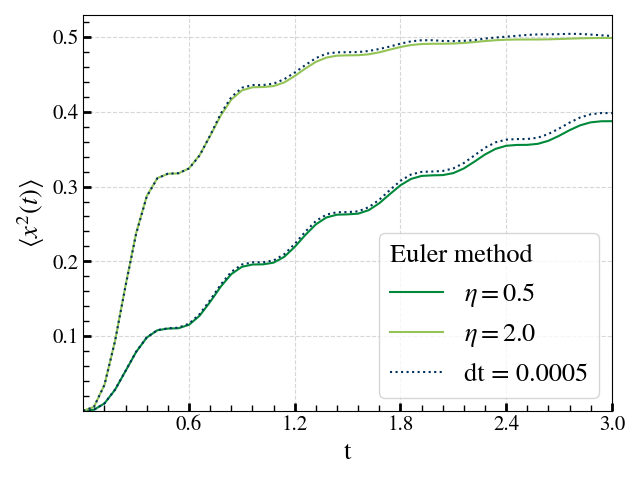
\includegraphics[width=0.95\linewidth]{graphics/HO-Euler-0.0005.png}
		\end{subfigure}
		\begin{subfigure}{0.5\textwidth}
			\centering
			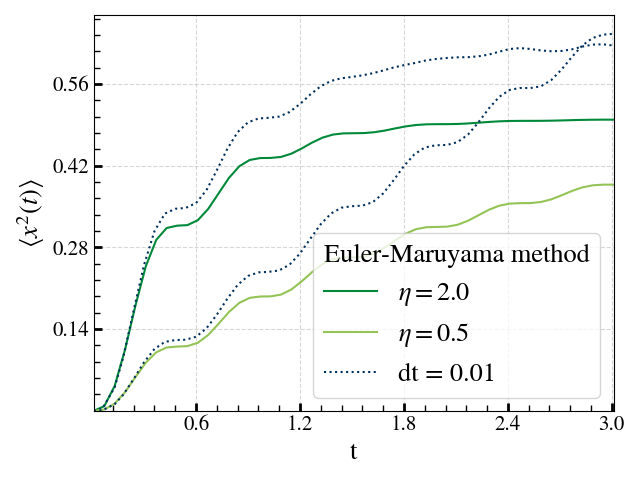
\includegraphics[width=0.95\linewidth]{graphics/HO-Euler-0.01.png}
		\end{subfigure}  \\
		\begin{subfigure}{0.5\textwidth}
			\centering
			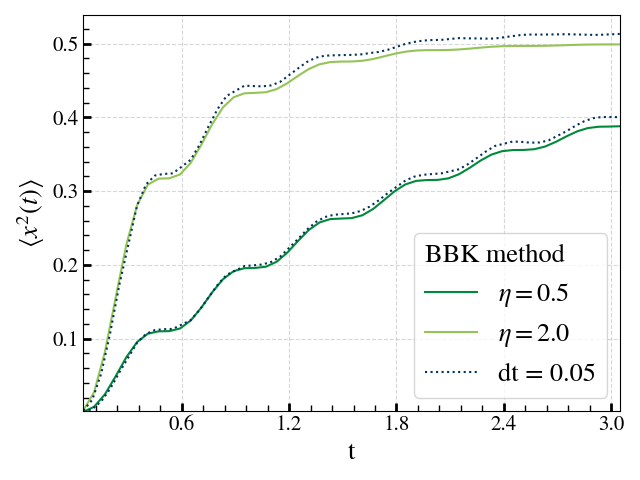
\includegraphics[width=0.95\linewidth]{graphics/HO-BBK-0.05.png}
		\end{subfigure}
		\begin{subfigure}{0.5\textwidth}
			\centering
			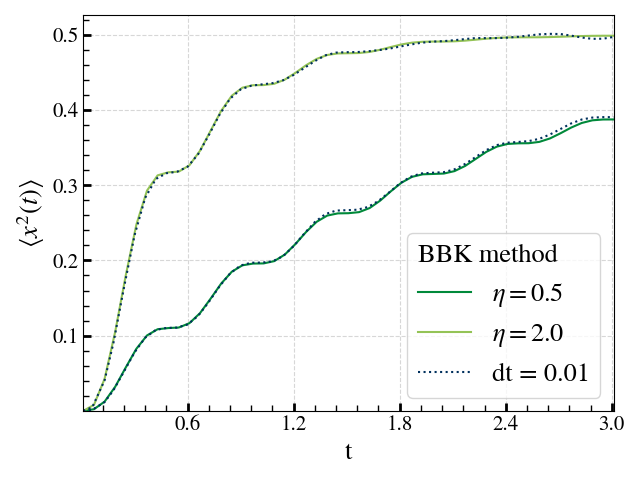
\includegraphics[width=0.95\linewidth]{graphics/HO-BBK-0.01.png}
		\end{subfigure}
		\caption{The calculated $\left \langle x^2 (t) \right \rangle $ of thermal harmonic oscillators are shown for different methods and step sizes. The green curves are the theoretical paths calculated from \eqref{Eq::MSD-HO} for $\omega^2 =	20$, $T	=	20$ and $m=1$.	The damping is denoted in the legend. The dotted lines are paths calculated from $10^5$ simulated realizations. The top plots are calculated using the Euler-Maruyama method and the bottom plots using the BBK	method. The Euler-Maruyama method with $\text{d}t =	0.0005$ shows comparable discretization errors as the BBK method with $\text{d}t =	0.05$, which is a difference of two orders of magnitude. For a step size of $\text{d}t = 0.01$, the BBK method shows virtually no discretization errors, while the Euler-Maruyama method strongly deviates from the theoretical curve.}
		\label{Fig::MSD-Comparison}
	\end{figure}
	\subsection{Two Interacting Particles in a Cosine Potential}
	The second benchmark has the purpose of verifying the correct behavior of the interaction as well as correct equilibration. We consider the one dimensional version of Eq. \eqref{Eq::XY-Hamilton-Field} for two sites, so particle-pairs in a cosine potential interacting via an XY interaction. The equilibrium distribution becomes a high dimensional function $p(\vartheta_1, \vartheta_2, \omega_1, \omega_2)$. We expect that this distribution relaxes to the equilibrium distribution of the Fokker-Planck equation, so the canonical distribution. A suitable representation achieved by integrating out the angular velocities and considering a cross section of a fixed interval $\left[\vartheta_2 - \tfrac{1}{2} \text{d} \vartheta_2, \vartheta_2 + \tfrac{1}{2} \text{d} \vartheta_2 \right]$.  \\
	
	In \autoref{Fig::Pair-Prob-Dist} we show cuts of the integrated probability density 
	\begin{equation}
		p(\vartheta_1, \vartheta_2) \text{d}\vartheta_2 =	\int_{} p(\vartheta_1, \vartheta_2, \omega_1, \omega_2) \text{d}\omega_2 \text{d}\omega_1\text{d}\vartheta_2,
	\end{equation}
	 with constant $\vartheta_2$. It is verified that simple interacting systems are driven to their equilibrium. The statistical- and discretization errors vanish for many samples and small step sizes $\text{d}\sigma$. Naturally, the 
	
	\begin{figure}[htp]
		\begin{subfigure}{0.5\textwidth}
			\centering
			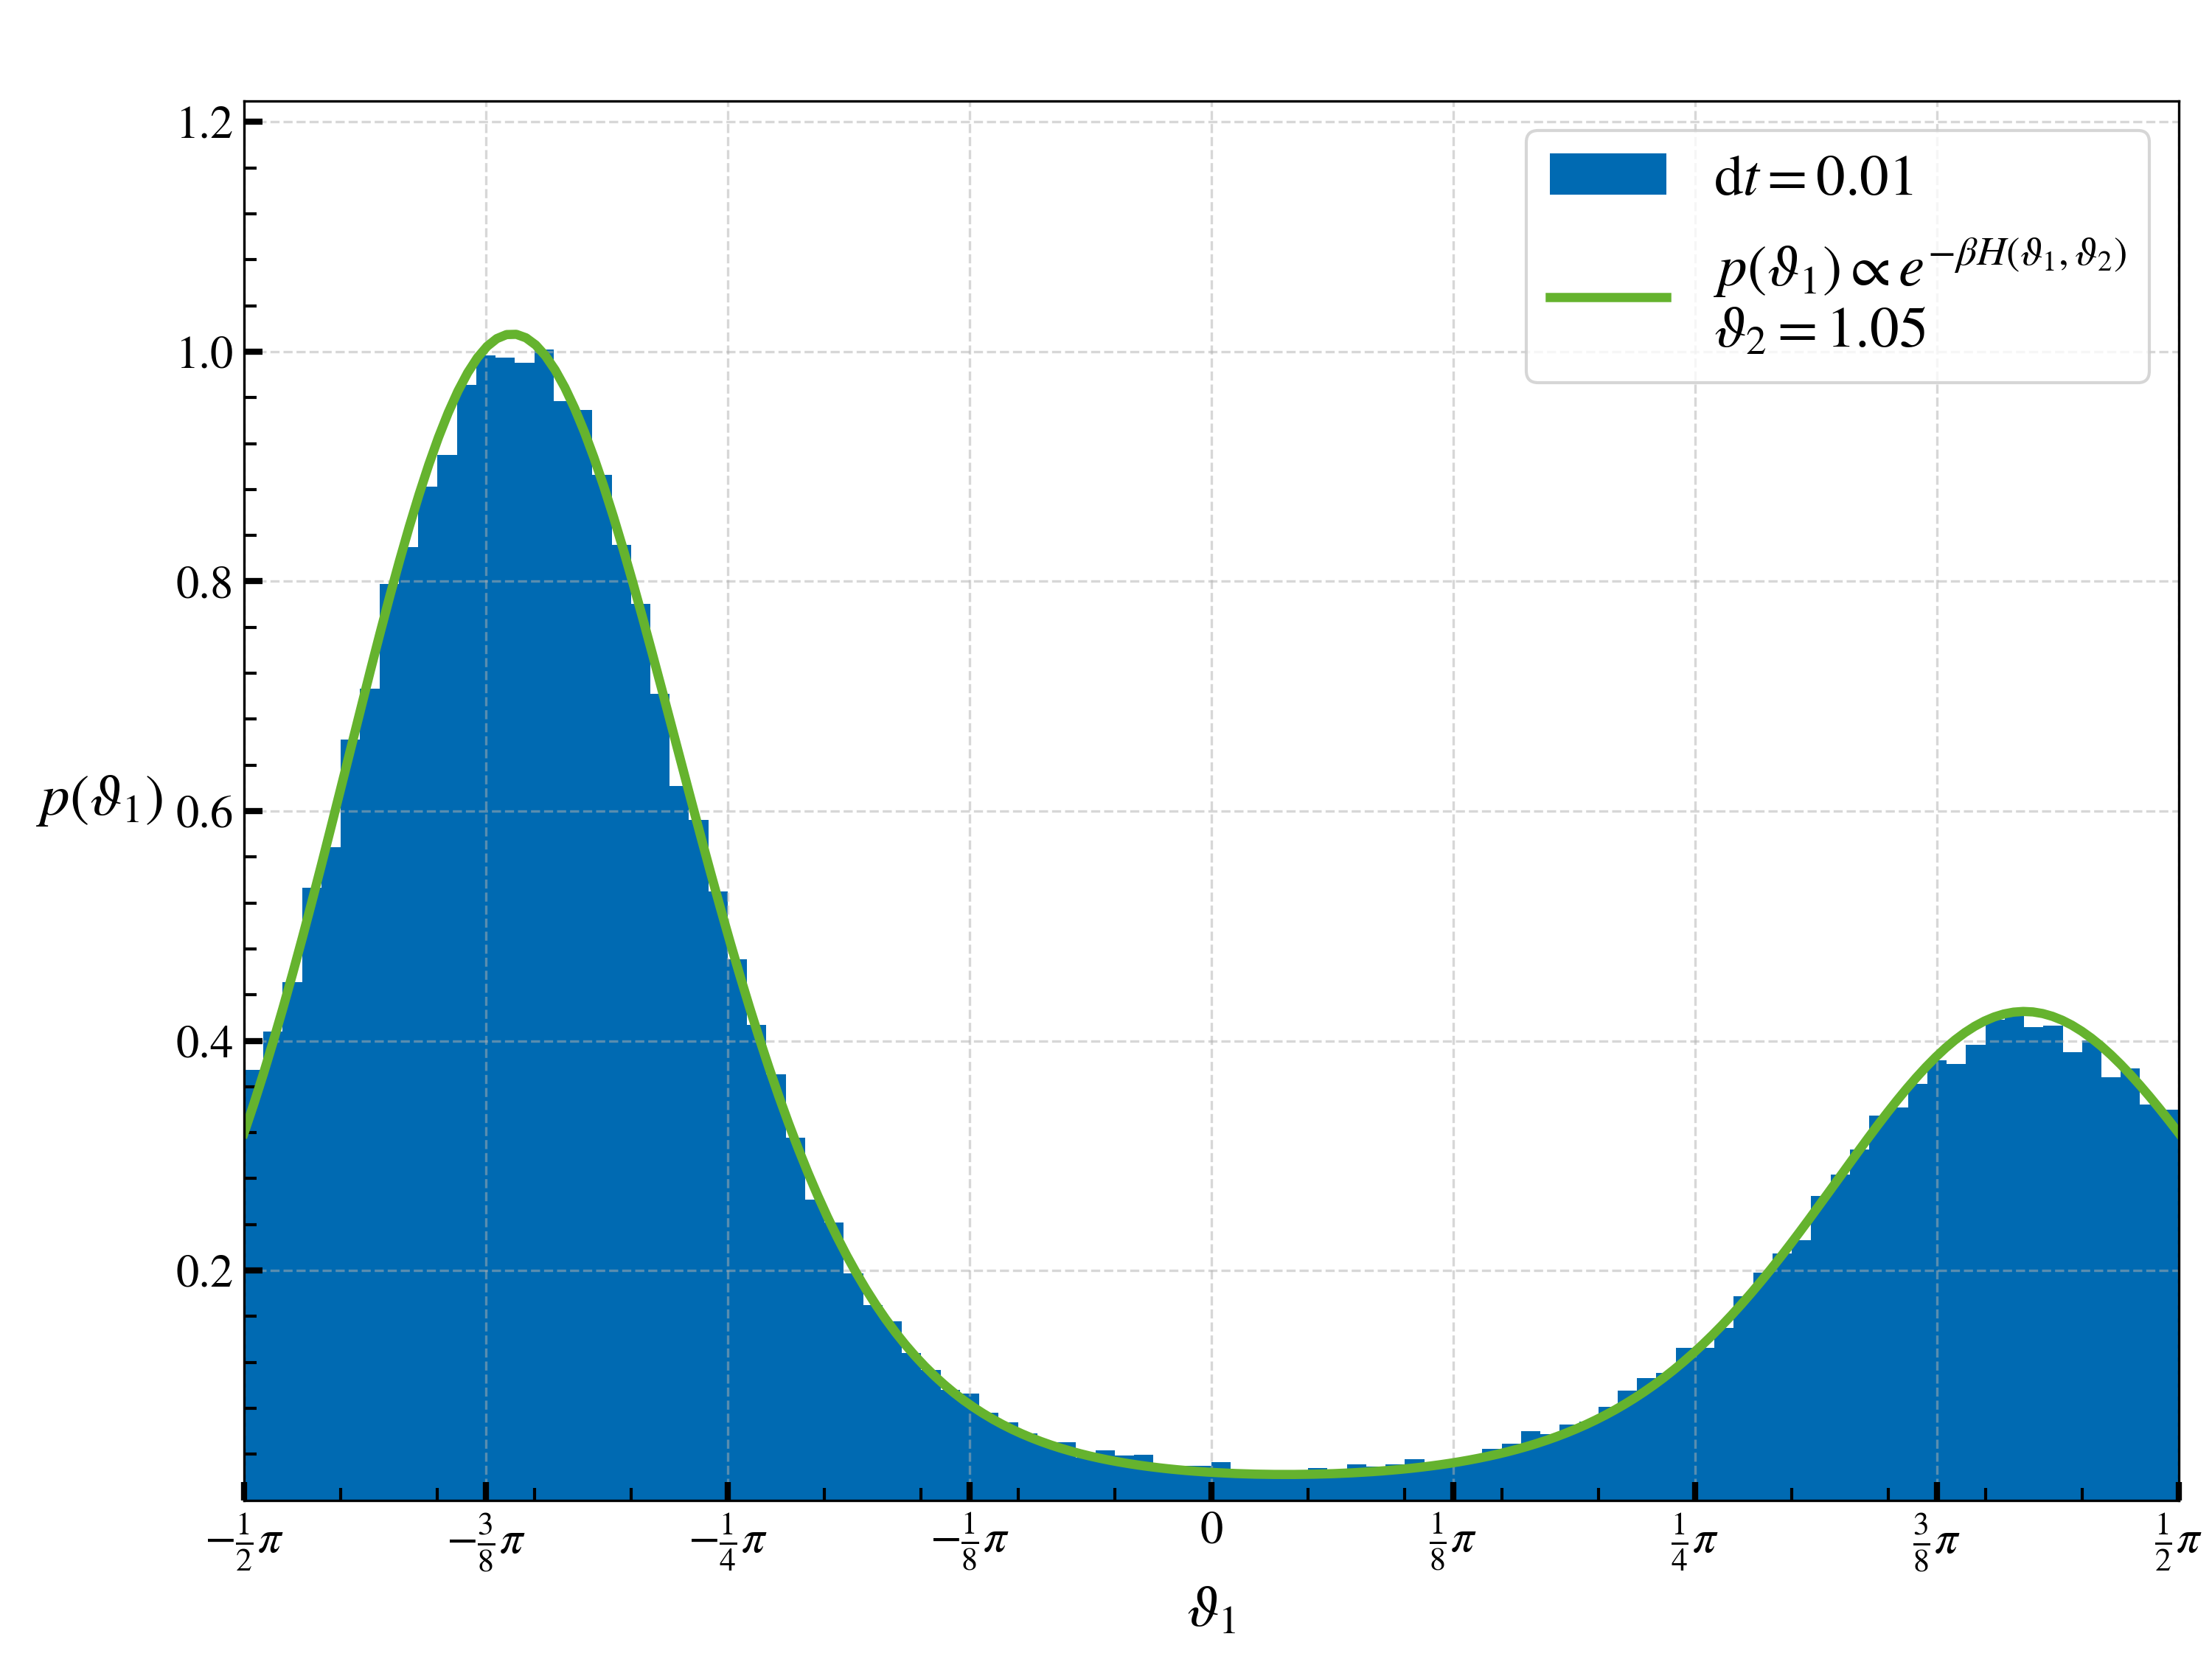
\includegraphics[width=0.8\linewidth]{graphics/eq-dist-0.01.png}
		\end{subfigure}
		\begin{subfigure}{0.5\textwidth}
			\centering
			\includegraphics[width=0.8\linewidth]{graphics/eq-dist-0.001.png}
		\end{subfigure} \\
		\begin{subfigure}{0.5\textwidth}
			\centering
			\includegraphics[width=0.8\linewidth]{graphics/eq-dist-0.02.png}
		\end{subfigure}
		\begin{subfigure}{0.5\textwidth}
			\centering
			\includegraphics[width=0.8\linewidth]{graphics/eq-dist-0.05.png}
		\end{subfigure} \\
		\begin{subfigure}{0.5\textwidth}
			\centering
			\includegraphics[width=0.8\linewidth]{graphics/eq-dist-0.0001.png}
		\end{subfigure}
		\begin{subfigure}{0.5\textwidth}
			\centering
			\includegraphics[width=0.8\linewidth]{graphics/eq-dist-0.00001.png}
		\end{subfigure} 
		\caption{The integrated probability distribution $p(\vartheta_1, \vartheta_2)\text{d}\vartheta_2$ of particle pairs described by Eq. \eqref{Eq::XY-Hamilton-Field} around constant $\vartheta_2$ is shown. The used parameters for (a) - (d) were $j =	40,~ \rho =	100,~ p=2.5,~ \eta =	1$ and $\kappa = 100$. The interactions and temperatures are chosen to be larger than in the actual simulation on purpose. The green curve is the canonical distribution. The blue bins are calculated from $5 \cdot 10^5$ simulated pair paths by counting particles in $\left[\vartheta_2 - \tfrac{1}{2} \text{d} \vartheta_2, \vartheta_2 + \tfrac{1}{2} \text{d} \vartheta_2 \right]$ and binning them into $100$ sections. It was made sure that the systems were completely relaxed, meaning that the effects of the starting position vanished and the shape of the probability distribution did not change anymore. The integrations were performed using the BBK method. The BBK method again shows no discretization errors for $\text{d}\sigma=0.01$. Slightly larger step sizes of $\text{d}t =	0.02$ already produce visually recognizable deviations. Simulations with $\text{d}\sigma = 0.05 $ deviate strongly. Almost no improvement is achieved by reducing the step size to $\text{d}t =	0.001$. How small the step size has to be naturally depends on the system at hand, therefore the benchmark is repeated for parameters in the dimensions of the experimental coupling constants in (e) and (f). The coupling constants of the previous computations are multiplied with $10^4$. For parameters in this order of magnitude, step sizes should not be larger than $\text{d}\sigma = 10^{-5}$.}
		\label{Fig::Pair-Prob-Dist}
	\end{figure}
	
	\section{Correlation Length Calculation} \label{Section::Corr-Length-Calculation}
	The two-point equal time correlation function of the XY model in two dimensions is defined as
	\begin{equation}
		C(x, y) = \langle \vec{s}_{0,0} \vec{s}_{x, y} \rangle ~.
	\end{equation}
	The brackets $\langle~\cdot~\rangle$ denote the ensemble average
	\begin{equation}
		\langle \vec{s}_{0,0} \vec{s}_{x, y} \rangle  = \frac{1}{Z} \int \prod_i d\vartheta_i \vec{s}_{0,0} \vec{s}_{x, y} e^{- \beta H(\{\vartheta\})}
	\end{equation}	
	The correlation function decays exponentially for large distances above the critical temperature \cite{kosterlitz1974critical, amit1980renormalisation}, following	 
	\begin{equation} \label{Eq::corr-func-decay-above-Tc}
		C(x, y) \sim e^{-r(x,y) /	\xi(x,y)} \qquad \text{with} \qquad r =	\sqrt{x^2 + y^2}.
	\end{equation}
	This is the definition of the correlation length $\xi$. The correlation length is a measure for the length scale over which perturbations of a system relax in space. We are mainly interested in the correlation lengths in the directions along and across the dimer row and therefore define the correlation functions in these directions as
	\begin{align} \label{Eq::Corr-Func-asymptotic}
		C_\perp(x) =  \langle \vec{s}_{0,0} \vec{s}_{x, 0} \rangle \sim e^{-x /	\xi_\perp} \qquad \text{and} \qquad
		C_\parallel(y) =  \langle \vec{s}_{0,0} \vec{s}_{0, y} \rangle \sim e^{-y /	\xi_\parallel}.
	\end{align}
	Consider the Fourier transforms of $C_\delta(r)$
	\begin{equation}  \label{Eq::FT-Corr-delta}
		S_\delta(k) = \sum_r^{N_\delta - 1} C_\delta (r) e^{-2\pi i \frac{kr}{N_\delta}}~,
	\end{equation}
	with $N_\delta$ being the number of lattice sites in the direction of $\delta$. Set in the following $\delta =	\perp$. The Fourier transform becomes 
	\begin{equation} \label{Eq::FT-of-Corr-perp}
		\begin{split}
			S_\perp(k) = \sum_x^{N_\perp - 1} C_\perp (x) e^{-2\pi i \frac{kx}{N_\perp}} =\sum_x^{N_\perp - 1} \langle \vec{s}_{0,0} \vec{s}_{x, 0} \rangle e^{-2\pi i \frac{kx}{N_\perp}} = ~&\sum_x^{N_\perp - 1} \langle s^0_{0,0} s_{x, 0}^0 \rangle e^{-2\pi i \frac{kx}{N_\perp}} \\
			+&\sum_x^{N_\perp - 1} \langle s_{0,0}^1  \
			s_{x, 0}^1 \rangle e^{-2\pi i \frac{kx}{N_\perp}}.
		\end{split}
	\end{equation}
	The ensemble average can be computed by a sum over an infinite lattice
	\begin{equation} \label{Eq::Ensemble-Avg-as-mean}
		\langle s^\kappa_{0,0} s_{x, 0}^\kappa \rangle =	\lim\limits_{N_\perp \rightarrow \infty} \lim\limits_{N_\parallel \rightarrow \infty} \frac{1}{N_\perp N_\parallel} \sum_{i =	0}^{N_\perp} \sum_{j=0}^{N_\parallel}   s^\kappa_{i,j} s_{i + x, j}^\kappa~,
	\end{equation}
	where $\kappa$ denotes the spin component. An approximation is possible by using a finite lattice with large dimensions $N_\delta$. Inserting Eq.~\eqref{Eq::Ensemble-Avg-as-mean} into Eq.~\eqref{Eq::FT-of-Corr-perp} and replacing the sum $\sum_x$ with a sum over $q =	i +x$ yields
	\begin{equation} \label{Eq::FT-Corr-Delta}
		S_\perp(k) = \frac{1}{N_\perp N_\parallel}  \sum_{\kappa,q,i,j}^{}   s^\kappa_{i,j} s_{q, j}^\kappa e^{-2\pi i \frac{k(q-i)}{N_\perp}} =	\frac{1}{N_\perp N_\parallel}  \sum_{\kappa,q,i,j}^{}  \left(\sum_{p=0}^{N_\parallel} \delta_{p,j} \right) s^\kappa_{i,j} s_{q, p}^\kappa e^{-2\pi i \frac{k(q-i)}{N_\perp}}~.
	\end{equation}
	In the second step we have inserted a productive one in the form of  a sum over a Kronecker delta. The Kronecker delta can be written as a sum over complex exponentials
	\begin{equation}
		\delta_{p,j} =	\frac{1}{N_\parallel} \sum_{l=1}^{N_\parallel} e^{2 \pi i \frac{l(j - p)}{N_\parallel}}~.
	\end{equation}
	Inserting this representation into Eq.~\eqref{Eq::FT-Corr-Delta} gives
	\begin{equation}
		\begin{split}
			S_\perp(k) &=	\frac{1}{N_\perp N_\parallel^2} \sum_l \sum_\kappa \sum_{q,p,i,j} s^\kappa_{i,j} s_{q, p}^\kappa e^{-2\pi i \frac{k(q-i)}{N_\perp}} e^{2 \pi i \frac{l(p - j)}{N_\parallel}} \\
			&=	\frac{1}{N_\perp N_\parallel^2} \sum_l \sum_\kappa \left(\sum_{i,j} s^\kappa_{i,j} e^{2\pi i \left(\frac{ki}{N_\perp} + \frac{lj}{N_\parallel} \right)} \right) \left(\sum_{q,p} s_{q, p}^\kappa e^{-2 \pi i \left( \frac{kq}{N_\perp} + \frac{lp}{N_\parallel} \right)} \right)~.
		\end{split}
	\end{equation}
	The expressions in the parentheses are the Fourier transforms $\tilde{s}_{k,l}^\kappa$, or respectively the conjugated Fourier transform, of the $s_{i,j}^\kappa$ lattice:
	\begin{equation} \label{Eq::S-as-lattice-FT}
		\begin{split}
			S_\perp(k) &=	\frac{1}{N_\perp N_\parallel^2} \sum_l \sum_\kappa \left(\tilde{s}_{k,l}^\kappa\right)^* \tilde{s}_{k,l}^\kappa \\
			&= \frac{1}{N_\perp N_\parallel^2} \left( \sum_l |\tilde{s}_{k,l}^0|^2  + \sum_l |\tilde{s}_{k,l}^1|^2\right)~.
		\end{split}
	\end{equation}
	This way we can calculate $S_\perp(k)$ by calculating the two dimensional Fourier transforms of the lattices $s_{i,j}^0 = \cos \vartheta_{i,j}	$ and $s_{i,j}^1 =	\sin \vartheta_{i,j}$.
	The analogue result is valid for $S_\parallel(k)$. \\
	
	To eventually extract the correlation length, we consider again Eq.~\eqref{Eq::FT-Corr-Delta} and insert the asymptotic behavior of $C_\delta (r)$  Eq.~\eqref{Eq::Corr-Func-asymptotic} to obtain
	\begin{equation} \label{Eq::Lorentzian-Peak}
		S_\delta(k) \sim \sum_r^{N_\delta - 1} e^{-|r| /	\xi_\delta} e^{-2\pi i \frac{kr}{N_\delta}} = \frac{2 \xi_\delta}{1 + 4 \pi^2 \xi_\delta^2 k^2}	~,
	\end{equation}
	showing that $S_\delta(k)$ behaves like a Lorentzian function around $k=0$. Calculating $S_\delta(k)$ by means of Eq.~\eqref{Eq::S-as-lattice-FT} and fitting to the Lorentzian Eq.~\eqref{Eq::Lorentzian-Peak} yields $\xi_\delta$ as fitting parameter. Since Eq. \eqref{Eq::corr-func-decay-above-Tc} is valid for large $r$, it is important to only fit the peak of $S_\delta(k)$ around $k = 0$. Correlations below the critical temperature in the Ising universality class can be shown \cite{mccoy1973two} to decay like
	\begin{equation}
		C(x, y) \sim  c + e^{-r(x,y) /	\xi(x,y)},
	\end{equation}
	with a constant $c$. When performing the Fourier transform, this constant contributes to a delta peak at $k = 0$. To correctly extract correlation lengths below $T_c$, the $S_\delta(k)$ value has to be cut.	
	\section{Error Calculation on Moving Averages} \label{Section::Error-Calc}	
	An average $\overline{f}$ that is calculated by the means of Eq.~\eqref{Eq::ensemble-average-calculation} has a non trivial relationship with it's variance $\sigma_{\overline{f}}$ \cite{madras1988pivot}. The reason for this is that $f(t)$ and $f(t + mdt)$ might be, and most probably are, correlated. Observables at different times are dependent on each other  and have to be treated accordingly. \\
	
	The average $\overline{f}$ of a time series $f(s)$ is calculated as
	\begin{equation}
		\overline{f} = f_\tau =	\frac{1}{\tau} \int_0^{\tau} ds f(s) ~,
	\end{equation}
	with $\tau$ being the duration of the observation. To estimate the error on $f_\tau$ we consider the variance of the average $f_\tau$ \cite{frenkel2023understanding, anderson2011statistical}
	\begin{equation} \label{Eq::Time-Series-Var}
		\begin{split}
			\sigma_{\overline{f}}^2 &=	\left \langle f_\tau^2 \right \rangle - \left \langle f_\tau \right \rangle^2 \\
			&\approx \frac{1}{\tau} \int_{-\infty}^{\infty} \text{d}t~C_f(t),
		\end{split}
	\end{equation}
	with $C_f(t)$ being the autocorrelation or time correlation function
	\begin{equation} \label{Eq::Autorcorrlation-Time}
		C_f(t) =	\left \langle f(s) f(s + t) \right \rangle - \left \langle f(s) \right \rangle^2~.
	\end{equation}
	The step performed in Eq.~\eqref{Eq::Time-Series-Var} is valid in the limit of $\tau \gg \tau_C$, so that the sampling time $\tau$ is much larger than the characteristic decay time of the autocorrelation function $\tau_C$. $\tau_C$ is defined as
	\begin{equation} \label{Eq::Autocorrelation-Time}
		\tau_C = \frac{1}{2}	\int_{-\infty}^{\infty} \text{d}t~C_f(t) /	C_f(0)~.
	\end{equation}
	The decay time $\tau_C$ is also called the \textbf{integrated autocorrelation time}. So that we can express $\sigma_{\overline{f}}^2$ in terms of $\tau_C$
	\begin{equation}
		\sigma_{\overline{f}}^2 =	\frac{2\tau_C}{\tau} C_f(0)~.
	\end{equation}
	Looking at Eq.~\eqref{Eq::Autocorrlation-Time}, we can see that $C_f(0)$ reduces to the variance of $f$
	\begin{equation}
		C_f(0) =	\sigma_f^2~.
	\end{equation}
	Rewriting $\tau =	n_s \tau_s$ with $n_s$ being the number of measured samples and $\tau_s$ being the time between the samples, the variance of the mean $\overline{f}$ can be expressed as
	\begin{equation}
		\sigma_{\overline{f}}^2 =	\frac{2 \tau_C}{\tau_s} \frac{\sigma_f^2}{n_s} ~,
	\end{equation}
	revealing that the variance of $\overline{f}$ is by a factor of $\frac{2 \tau_c}{\tau_s}$ larger than the naive approach of uncorrelated measurements would yield. Since it is practically not possible to integrate Eq.~\eqref{Eq::Autorcorrlation-Time} from $-\infty$ to $\infty$,   we approximate $\tau_c$ by
	\begin{equation}
		\tau_C \approx \frac{1}{2} \int_{-\tau/2}^{\tau/2} \text{d}t~C_f(t) /	C_f(0)~.
	\end{equation}
	
	\section{The Role of $p$} \label{Section::role-p}
	The role of the parameter $p$ of \eqref{Eq::XY-Hamilton-Field} fell a bit short in previous discussion because of a lack of time. Put simply, $p$ determines where the minimum of the symmetry breaking field lies, but also influences the height of the potential barrier as can be seen in \autoref{Fig::XY-Silicon-Potential}. It has been briefly tested that variation of $p$ does not change the critical behavior of the system. Things like the phase diagram  might have to be reformulated in terms of the potential barrier	
	\begin{equation}
		E_B =	h \left(1 + \cos\left(\frac{\pi}{2} p \right)\right),
	\end{equation}
	if one were to change p. \\
	
	The equilibrium position of the dimers is determined by the strength of repulsion $J_\parallel$ and $J_\perp$, the amplitude of the symmetry breaking field $h$ and the position of its minima determined by the parameter $p$. In the case of ferromagnetic interaction, the equilibrium position is solely determined by $p = \tfrac{18}{7} $ which yields the experimental equilibrium position of $\vartheta^* =	\tfrac{7}{18} \pi = 70^\circ$ (measuring from the z-Axis). We can also infer that $p > 2$ as $p=2$ means that the equilibrium position of the symmetry breaking field is at $\vartheta = \pi /	2$, corresponding to a horizontal dimer. Since we see from DFT calculations that even the buckling itself without any constraint on the configuration decreases the energy, this is not realistic. The two constrains conclude to $p \in \left[2, 2.57\right]$ Consider now a specific lattice site of a system in total equilibrium, meaning that the site's buckling angle is $\vartheta =	\vartheta^*$ and the buckling angle of all its neighbors is $\vartheta_{NN} =	- \vartheta^*$. The condition that $\tfrac{\partial H(\vartheta)}{\partial \vartheta} \Big |_{\vartheta =	\vartheta^*} =	0$ gives
	\begin{equation} \label{Eq::Equilibrium-Position}
		-4 \sin(4 \vartheta^*) \left(\frac{J_\parallel + J_\perp}{h}\right) =	p \sin \left(\vartheta^* p\right)~.
	\end{equation}
	This transcendental equation for $p$ in dependence of the coupling parameters and the desired equilibrium angle is not guaranteed to have a solution. 	The left hand side is unbound but the right hand side is bound by $p$. For the experimental values we find
	\begin{equation}
		\frac{J_\parallel + J_\perp}{h} < \frac{1}{3}~,
	\end{equation}
	so that it is even possible to find a $p$ that reproduces the experimental equilibrium position.

	\section{Soft- and Hardware}
	\begin{table}[h]
		\centering
		\caption{The details and version numbers to the used soft- and hardware are listed.}
		\renewcommand{\arraystretch}{1.7}
		\begin{tabular}{l l }
			\toprule
			Tool $\qquad \qquad $& Version number \\
			\midrule
			Cuda &  $~$\\
			cuRAND & 11.2 \\
			cuFFT & $~$\\
			\midrule
			GCC & 10.2.0 \\
			C++ & C++17 \\
			Boost & 1.78.0 \\					
			\midrule
			OS & CentOS Linux 7.9.2009 \\
			CPU & Intel(R) Xeon(R) Gold 6148 \\
			GPU & Nvidia P100, V100, A100 \\
			\bottomrule
		\end{tabular}
		\label{Table::Hardware-Software}
	\end{table}

	\bibliographystyle{plain}
	\bibliography{references.bib}
	
	% Danksagung
	\clearpage
	\pagestyle{empty}
	\minisec{Acknowledgement}
	I would like to thank Prof. Schützhold for providing me with the opportunity to write this thesis at the Helmholtz-Zentrum Dresden-Rossendorf, opening up insights into the large research collaboration CRC 1242. I would like to thank Dr. Gernot Schaller as well as Dr. Friedemann Queisser for their excellent supervision during this project. Our weekly meetings acted as signposts on the path that eventually led to this work. I would like to thank Dr. Christian Kohlfürst for always caring about IT- and organizational matters and for exquisite company in the office. Also, I would like to thank Prof. Roland Ketzmerick for agreeing to review my thesis. \\
	
	My deepest gratitude goes towards Kathi for supplying me with nutritious and delicious meals, especially in the finishing phase of this project. Without her, this level of investment would not have been possible.  I would like to thank Julian and Mau for helpful suggestions and proofreading. I want to thank Kira for employing her english expertise to check my spelling and grammer. Finally, I would like to thank my brother Martin and Adrian for their generous self-sacrifice, offering to proofread 100 pages of a theoretical physics master's thesis.
	
	% Erklärung
	\clearpage
	\thispagestyle{empty}
	\minisec{Erklärung}\vspace*{1.5em}
	
	Hiermit erkläre ich, dass ich diese Arbeit im Rahmen der Betreuung am Institut
	für Theoretische Physik ohne unzulässige Hilfe Dritter verfasst und alle Quellen als solche gekennzeichnet habe.
	
	\vspace*{45em}
	
	Andreas Weitzel \par
	Dresden, April 2024
	
\end{document}
